% **************************************************************************************************************
% A Classic Thesis Style
% An Homage to The Elements of Typographic Style
%
% Copyright (C) 2015 André Miede http://www.miede.de
%
% If you like the style then I would appreciate a postcard. My address 
% can be found in the file ClassicThesis.pdf. A collection of the 
% postcards I received so far is available online at 
% http://postcards.miede.de
%
% License:
% This program is free software; you can redistribute it and/or modify
% it under the terms of the GNU General Public License as published by
% the Free Software Foundation; either version 2 of the License, or
% (at your option) any later version.
%
% This program is distributed in the hope that it will be useful,
% but WITHOUT ANY WARRANTY; without even the implied warranty of
% MERCHANTABILITY or FITNESS FOR A PARTICULAR PURPOSE.  See the
% GNU General Public License for more details.
%
% You should have received a copy of the GNU General Public License
% along with this program; see the file COPYING.  If not, write to
% the Free Software Foundation, Inc., 59 Temple Place - Suite 330,
% Boston, MA 02111-1307, USA.
%
% **************************************************************************************************************
\RequirePackage{fix-cm} % fix some latex issues see: http://texdoc.net/texmf-dist/doc/latex/base/fixltx2e.pdf

\documentclass[ twoside,openright,titlepage,numbers=noenddot,headinclude,%1headlines,% letterpaper a4paper
                footinclude=true,cleardoublepage=empty,abstractoff, % <--- obsolete, remove (todo)
                BCOR=5mm,paper=a4,fontsize=11pt,%11pt,a4paper,%
                ngerman,american,%
                ]{scrreprt}

%********************************************************************
% Note: Make all your adjustments in here
%*******************************************************

% ****************************************************************************************************
% classicthesis-config.tex 
% formerly known as loadpackages.sty, classicthesis-ldpkg.sty, and classicthesis-preamble.sty 
% Use it at the beginning of your ClassicThesis.tex, or as a LaTeX Preamble 
% in your ClassicThesis.{tex,lyx} with % ****************************************************************************************************
% classicthesis-config.tex 
% formerly known as loadpackages.sty, classicthesis-ldpkg.sty, and classicthesis-preamble.sty 
% Use it at the beginning of your ClassicThesis.tex, or as a LaTeX Preamble 
% in your ClassicThesis.{tex,lyx} with % ****************************************************************************************************
% classicthesis-config.tex 
% formerly known as loadpackages.sty, classicthesis-ldpkg.sty, and classicthesis-preamble.sty 
% Use it at the beginning of your ClassicThesis.tex, or as a LaTeX Preamble 
% in your ClassicThesis.{tex,lyx} with \input{classicthesis-config}
% ****************************************************************************************************  
% If you like the classicthesis, then I would appreciate a postcard. 
% My address can be found in the file ClassicThesis.pdf. A collection 
% of the postcards I received so far is available online at 
% http://postcards.miede.de
% ****************************************************************************************************


% ****************************************************************************************************
% 0. Set the encoding of your files. UTF-8 is the only sensible encoding nowadays. If you can't read
% äöüßáéçèê∂åëæƒÏ€ then change the encoding setting in your editor, not the line below. If your editor
% does not support utf8 use another editor!
% ****************************************************************************************************
\PassOptionsToPackage{utf8}{inputenc}
	\usepackage{inputenc}

% ****************************************************************************************************
% 1. Configure classicthesis for your needs here, e.g., remove "drafting" below 
% in order to deactivate the time-stamp on the pages
% ****************************************************************************************************
\PassOptionsToPackage{eulerchapternumbers,listings,%
					 pdfspacing,floatperchapter,%linedheaders,%
					 subfig,beramono,eulermath}{classicthesis}                                        
% ********************************************************************
% Available options for classicthesis.sty 
% (see ClassicThesis.pdf for more information):
% drafting
% parts nochapters linedheaders
% eulerchapternumbers beramono eulermath pdfspacing minionprospacing
% tocaligned dottedtoc manychapters
% listings floatperchapter subfig
% ********************************************************************


% ****************************************************************************************************
% 2. Personal data and user ad-hoc commands
% ****************************************************************************************************
\newcommand{\myTitle}{Black hole masses and outflows in high redshift quasars\xspace}
\newcommand{\mySubtitle}{An Homage to The Elements of Typographic Style\xspace}
\newcommand{\myDegree}{Doktor-Ingenieur (Dr.-Ing.)\xspace}
\newcommand{\myName}{Liam Coatman\xspace}
\newcommand{\myProf}{Put name here\xspace}
\newcommand{\myOtherProf}{Put name here\xspace}
\newcommand{\mySupervisor}{Put name here\xspace}
\newcommand{\myFaculty}{Put data here\xspace}
\newcommand{\myDepartment}{Put data here\xspace}
\newcommand{\myUni}{Put data here\xspace}
\newcommand{\myLocation}{Saarbrücken\xspace}
\newcommand{\myTime}{September 2015\xspace}
\newcommand{\myVersion}{version 4.2\xspace}

% ********************************************************************
% Setup, finetuning, and useful commands
% ********************************************************************
\newcounter{dummy} % necessary for correct hyperlinks (to index, bib, etc.)
\newlength{\abcd} % for ab..z string length calculation
\providecommand{\mLyX}{L\kern-.1667em\lower.25em\hbox{Y}\kern-.125emX\@}
\newcommand{\ie}{i.\,e.}
\newcommand{\Ie}{I.\,e.}
\newcommand{\eg}{e.\,g.}
\newcommand{\Eg}{E.\,g.} 
% ****************************************************************************************************


% ****************************************************************************************************
% 3. Loading some handy packages
% ****************************************************************************************************
% ******************************************************************** 
% Packages with options that might require adjustments
% ******************************************************************** 
%\PassOptionsToPackage{ngerman,american}{babel}   % change this to your language(s)
% Spanish languages need extra options in order to work with this template
%\PassOptionsToPackage{spanish,es-lcroman}{babel}
	\usepackage{babel}                  

\usepackage{csquotes}
\PassOptionsToPackage{%
    %backend=biber, %instead of bibtex
	backend=bibtex8,bibencoding=ascii,%
	language=auto,%
	% style=numeric-comp,%
    style=authoryear, % Author 1999, 2010
    % bibstyle=authoryear,dashed=false, % dashed: substitute rep. author with ---
    sorting=nyt, % name, year, title
    maxbibnames=10, % default: 3, et al.
    %backref=true,%
    natbib=true % natbib compatibility mode (\citep and \citet still work)
}{biblatex}
    \usepackage{biblatex}

\PassOptionsToPackage{fleqn}{amsmath}       % math environments and more by the AMS 
    \usepackage{amsmath}

% ******************************************************************** 
% General useful packages
% ******************************************************************** 
\PassOptionsToPackage{T1}{fontenc} % T2A for cyrillics
    \usepackage{fontenc}     
\usepackage{textcomp} % fix warning with missing font shapes
\usepackage{scrhack} % fix warnings when using KOMA with listings package          
\usepackage{xspace} % to get the spacing after macros right  
\usepackage{mparhack} % get marginpar right
\usepackage{fixltx2e} % fixes some LaTeX stuff --> since 2015 in the LaTeX kernel (see below)
%\usepackage[latest]{latexrelease} % will be used once available in more distributions (ISSUE #107)
\PassOptionsToPackage{printonlyused,smaller}{acronym} 
    \usepackage{acronym} % nice macros for handling all acronyms in the thesis
    %\renewcommand{\bflabel}[1]{{#1}\hfill} % fix the list of acronyms --> no longer working
    %\renewcommand*{\acsfont}[1]{\textsc{#1}} 
    \renewcommand*{\aclabelfont}[1]{\acsfont{#1}}
% ****************************************************************************************************


% ****************************************************************************************************
% 4. Setup floats: tables, (sub)figures, and captions
% ****************************************************************************************************
\usepackage{tabularx} % better tables
    \setlength{\extrarowheight}{3pt} % increase table row height
\newcommand{\tableheadline}[1]{\multicolumn{1}{c}{\spacedlowsmallcaps{#1}}}
\newcommand{\myfloatalign}{\centering} % to be used with each float for alignment
\usepackage{caption}
% Thanks to cgnieder and Claus Lahiri
% http://tex.stackexchange.com/questions/69349/spacedlowsmallcaps-in-caption-label
% [REMOVED DUE TO OTHER PROBLEMS, SEE ISSUE #82]    
%\DeclareCaptionLabelFormat{smallcaps}{\bothIfFirst{#1}{~}\MakeTextLowercase{\textsc{#2}}}
%\captionsetup{font=small,labelformat=smallcaps} % format=hang,
\captionsetup{font=small} % format=hang,
\usepackage{subfig}  
% ****************************************************************************************************


% ****************************************************************************************************
% 5. Setup code listings
% ****************************************************************************************************
\usepackage{listings} 
%\lstset{emph={trueIndex,root},emphstyle=\color{BlueViolet}}%\underbar} % for special keywords
\lstset{language=[LaTeX]Tex,%C++,
    morekeywords={PassOptionsToPackage,selectlanguage},
    keywordstyle=\color{RoyalBlue},%\bfseries,
    basicstyle=\small\ttfamily,
    %identifierstyle=\color{NavyBlue},
    commentstyle=\color{Green}\ttfamily,
    stringstyle=\rmfamily,
    numbers=none,%left,%
    numberstyle=\scriptsize,%\tiny
    stepnumber=5,
    numbersep=8pt,
    showstringspaces=false,
    breaklines=true,
    %frameround=ftff,
    %frame=single,
    belowcaptionskip=.75\baselineskip
    %frame=L
} 
% ****************************************************************************************************             


% ****************************************************************************************************
% 6. PDFLaTeX, hyperreferences and citation backreferences
% ****************************************************************************************************
% ********************************************************************
% Using PDFLaTeX
% ********************************************************************
\PassOptionsToPackage{pdftex,hyperfootnotes=false,pdfpagelabels}{hyperref}
    \usepackage{hyperref}  % backref linktocpage pagebackref
\pdfcompresslevel=9
\pdfadjustspacing=1 
\PassOptionsToPackage{pdftex}{graphicx}
    \usepackage{graphicx} 
 

% ********************************************************************
% Hyperreferences
% ********************************************************************
\hypersetup{%
    %draft, % = no hyperlinking at all (useful in b/w printouts)
    colorlinks=true, linktocpage=true, pdfstartpage=3, pdfstartview=FitV,%
    % uncomment the following line if you want to have black links (e.g., for printing)
    %colorlinks=false, linktocpage=false, pdfstartpage=3, pdfstartview=FitV, pdfborder={0 0 0},%
    breaklinks=true, pdfpagemode=UseNone, pageanchor=true, pdfpagemode=UseOutlines,%
    plainpages=false, bookmarksnumbered, bookmarksopen=true, bookmarksopenlevel=1,%
    hypertexnames=true, pdfhighlight=/O,%nesting=true,%frenchlinks,%
    urlcolor=RoyalBlue, linkcolor=RoyalBlue, citecolor=RoyalBlue, %pagecolor=RoyalBlue,%
    %urlcolor=Black, linkcolor=Black, citecolor=Black, %pagecolor=Black,%
    pdftitle={\myTitle},%
    pdfauthor={\textcopyright\ \myName, \myUni, \myFaculty},%
    pdfsubject={},%
    pdfkeywords={},%
    pdfcreator={pdfLaTeX},%
    pdfproducer={LaTeX with hyperref and classicthesis}%
}   

% ********************************************************************
% Setup autoreferences
% ********************************************************************
% There are some issues regarding autorefnames
% http://www.ureader.de/msg/136221647.aspx
% http://www.tex.ac.uk/cgi-bin/texfaq2html?label=latexwords
% you have to redefine the makros for the 
% language you use, e.g., american, ngerman
% (as chosen when loading babel/AtBeginDocument)
% ********************************************************************
\makeatletter
\@ifpackageloaded{babel}%
    {%
       \addto\extrasamerican{%
			\renewcommand*{\figureautorefname}{Figure}%
			\renewcommand*{\tableautorefname}{Table}%
			\renewcommand*{\partautorefname}{Part}%
			\renewcommand*{\chapterautorefname}{Chapter}%
			\renewcommand*{\sectionautorefname}{Section}%
			\renewcommand*{\subsectionautorefname}{Section}%
			\renewcommand*{\subsubsectionautorefname}{Section}%     
                }%
       \addto\extrasngerman{% 
			\renewcommand*{\paragraphautorefname}{Absatz}%
			\renewcommand*{\subparagraphautorefname}{Unterabsatz}%
			\renewcommand*{\footnoteautorefname}{Fu\"snote}%
			\renewcommand*{\FancyVerbLineautorefname}{Zeile}%
			\renewcommand*{\theoremautorefname}{Theorem}%
			\renewcommand*{\appendixautorefname}{Anhang}%
			\renewcommand*{\equationautorefname}{Gleichung}%        
			\renewcommand*{\itemautorefname}{Punkt}%
                }%  
            % Fix to getting autorefs for subfigures right (thanks to Belinda Vogt for changing the definition)
            \providecommand{\subfigureautorefname}{\figureautorefname}%             
    }{\relax}
\makeatother


% ****************************************************************************************************
% 7. Last calls before the bar closes
% ****************************************************************************************************
% ********************************************************************
% Development Stuff
% ********************************************************************
\listfiles
%\PassOptionsToPackage{l2tabu,orthodox,abort}{nag}
%   \usepackage{nag}
%\PassOptionsToPackage{warning, all}{onlyamsmath}
%   \usepackage{onlyamsmath}

% ********************************************************************
% Last, but not least...
% ********************************************************************
\usepackage{classicthesis} 
% ****************************************************************************************************


% ****************************************************************************************************
% 8. Further adjustments (experimental)
% ****************************************************************************************************
% ********************************************************************
% Changing the text area
% ********************************************************************
%\linespread{1.05} % a bit more for Palatino
%\areaset[current]{312pt}{761pt} % 686 (factor 2.2) + 33 head + 42 head \the\footskip
%\setlength{\marginparwidth}{7em}%
%\setlength{\marginparsep}{2em}%

% ********************************************************************
% Using different fonts
% ********************************************************************
%\usepackage[oldstylenums]{kpfonts} % oldstyle notextcomp
%\usepackage[osf]{libertine}
%\usepackage[light,condensed,math]{iwona}
%\renewcommand{\sfdefault}{iwona}
%\usepackage{lmodern} % <-- no osf support :-(
%\usepackage{cfr-lm} % 
%\usepackage[urw-garamond]{mathdesign} <-- no osf support :-(
%\usepackage[default,osfigures]{opensans} % scale=0.95 
%\usepackage[sfdefault]{FiraSans}
% ****************************************************************************************************

% ****************************************************************************************************  
% If you like the classicthesis, then I would appreciate a postcard. 
% My address can be found in the file ClassicThesis.pdf. A collection 
% of the postcards I received so far is available online at 
% http://postcards.miede.de
% ****************************************************************************************************


% ****************************************************************************************************
% 0. Set the encoding of your files. UTF-8 is the only sensible encoding nowadays. If you can't read
% äöüßáéçèê∂åëæƒÏ€ then change the encoding setting in your editor, not the line below. If your editor
% does not support utf8 use another editor!
% ****************************************************************************************************
\PassOptionsToPackage{utf8}{inputenc}
	\usepackage{inputenc}

% ****************************************************************************************************
% 1. Configure classicthesis for your needs here, e.g., remove "drafting" below 
% in order to deactivate the time-stamp on the pages
% ****************************************************************************************************
\PassOptionsToPackage{eulerchapternumbers,listings,%
					 pdfspacing,floatperchapter,%linedheaders,%
					 subfig,beramono,eulermath}{classicthesis}                                        
% ********************************************************************
% Available options for classicthesis.sty 
% (see ClassicThesis.pdf for more information):
% drafting
% parts nochapters linedheaders
% eulerchapternumbers beramono eulermath pdfspacing minionprospacing
% tocaligned dottedtoc manychapters
% listings floatperchapter subfig
% ********************************************************************


% ****************************************************************************************************
% 2. Personal data and user ad-hoc commands
% ****************************************************************************************************
\newcommand{\myTitle}{Black hole masses and outflows in high redshift quasars\xspace}
\newcommand{\mySubtitle}{An Homage to The Elements of Typographic Style\xspace}
\newcommand{\myDegree}{Doktor-Ingenieur (Dr.-Ing.)\xspace}
\newcommand{\myName}{Liam Coatman\xspace}
\newcommand{\myProf}{Put name here\xspace}
\newcommand{\myOtherProf}{Put name here\xspace}
\newcommand{\mySupervisor}{Put name here\xspace}
\newcommand{\myFaculty}{Put data here\xspace}
\newcommand{\myDepartment}{Put data here\xspace}
\newcommand{\myUni}{Put data here\xspace}
\newcommand{\myLocation}{Saarbrücken\xspace}
\newcommand{\myTime}{September 2015\xspace}
\newcommand{\myVersion}{version 4.2\xspace}

% ********************************************************************
% Setup, finetuning, and useful commands
% ********************************************************************
\newcounter{dummy} % necessary for correct hyperlinks (to index, bib, etc.)
\newlength{\abcd} % for ab..z string length calculation
\providecommand{\mLyX}{L\kern-.1667em\lower.25em\hbox{Y}\kern-.125emX\@}
\newcommand{\ie}{i.\,e.}
\newcommand{\Ie}{I.\,e.}
\newcommand{\eg}{e.\,g.}
\newcommand{\Eg}{E.\,g.} 
% ****************************************************************************************************


% ****************************************************************************************************
% 3. Loading some handy packages
% ****************************************************************************************************
% ******************************************************************** 
% Packages with options that might require adjustments
% ******************************************************************** 
%\PassOptionsToPackage{ngerman,american}{babel}   % change this to your language(s)
% Spanish languages need extra options in order to work with this template
%\PassOptionsToPackage{spanish,es-lcroman}{babel}
	\usepackage{babel}                  

\usepackage{csquotes}
\PassOptionsToPackage{%
    %backend=biber, %instead of bibtex
	backend=bibtex8,bibencoding=ascii,%
	language=auto,%
	% style=numeric-comp,%
    style=authoryear, % Author 1999, 2010
    % bibstyle=authoryear,dashed=false, % dashed: substitute rep. author with ---
    sorting=nyt, % name, year, title
    maxbibnames=10, % default: 3, et al.
    %backref=true,%
    natbib=true % natbib compatibility mode (\citep and \citet still work)
}{biblatex}
    \usepackage{biblatex}

\PassOptionsToPackage{fleqn}{amsmath}       % math environments and more by the AMS 
    \usepackage{amsmath}

% ******************************************************************** 
% General useful packages
% ******************************************************************** 
\PassOptionsToPackage{T1}{fontenc} % T2A for cyrillics
    \usepackage{fontenc}     
\usepackage{textcomp} % fix warning with missing font shapes
\usepackage{scrhack} % fix warnings when using KOMA with listings package          
\usepackage{xspace} % to get the spacing after macros right  
\usepackage{mparhack} % get marginpar right
\usepackage{fixltx2e} % fixes some LaTeX stuff --> since 2015 in the LaTeX kernel (see below)
%\usepackage[latest]{latexrelease} % will be used once available in more distributions (ISSUE #107)
\PassOptionsToPackage{printonlyused,smaller}{acronym} 
    \usepackage{acronym} % nice macros for handling all acronyms in the thesis
    %\renewcommand{\bflabel}[1]{{#1}\hfill} % fix the list of acronyms --> no longer working
    %\renewcommand*{\acsfont}[1]{\textsc{#1}} 
    \renewcommand*{\aclabelfont}[1]{\acsfont{#1}}
% ****************************************************************************************************


% ****************************************************************************************************
% 4. Setup floats: tables, (sub)figures, and captions
% ****************************************************************************************************
\usepackage{tabularx} % better tables
    \setlength{\extrarowheight}{3pt} % increase table row height
\newcommand{\tableheadline}[1]{\multicolumn{1}{c}{\spacedlowsmallcaps{#1}}}
\newcommand{\myfloatalign}{\centering} % to be used with each float for alignment
\usepackage{caption}
% Thanks to cgnieder and Claus Lahiri
% http://tex.stackexchange.com/questions/69349/spacedlowsmallcaps-in-caption-label
% [REMOVED DUE TO OTHER PROBLEMS, SEE ISSUE #82]    
%\DeclareCaptionLabelFormat{smallcaps}{\bothIfFirst{#1}{~}\MakeTextLowercase{\textsc{#2}}}
%\captionsetup{font=small,labelformat=smallcaps} % format=hang,
\captionsetup{font=small} % format=hang,
\usepackage{subfig}  
% ****************************************************************************************************


% ****************************************************************************************************
% 5. Setup code listings
% ****************************************************************************************************
\usepackage{listings} 
%\lstset{emph={trueIndex,root},emphstyle=\color{BlueViolet}}%\underbar} % for special keywords
\lstset{language=[LaTeX]Tex,%C++,
    morekeywords={PassOptionsToPackage,selectlanguage},
    keywordstyle=\color{RoyalBlue},%\bfseries,
    basicstyle=\small\ttfamily,
    %identifierstyle=\color{NavyBlue},
    commentstyle=\color{Green}\ttfamily,
    stringstyle=\rmfamily,
    numbers=none,%left,%
    numberstyle=\scriptsize,%\tiny
    stepnumber=5,
    numbersep=8pt,
    showstringspaces=false,
    breaklines=true,
    %frameround=ftff,
    %frame=single,
    belowcaptionskip=.75\baselineskip
    %frame=L
} 
% ****************************************************************************************************             


% ****************************************************************************************************
% 6. PDFLaTeX, hyperreferences and citation backreferences
% ****************************************************************************************************
% ********************************************************************
% Using PDFLaTeX
% ********************************************************************
\PassOptionsToPackage{pdftex,hyperfootnotes=false,pdfpagelabels}{hyperref}
    \usepackage{hyperref}  % backref linktocpage pagebackref
\pdfcompresslevel=9
\pdfadjustspacing=1 
\PassOptionsToPackage{pdftex}{graphicx}
    \usepackage{graphicx} 
 

% ********************************************************************
% Hyperreferences
% ********************************************************************
\hypersetup{%
    %draft, % = no hyperlinking at all (useful in b/w printouts)
    colorlinks=true, linktocpage=true, pdfstartpage=3, pdfstartview=FitV,%
    % uncomment the following line if you want to have black links (e.g., for printing)
    %colorlinks=false, linktocpage=false, pdfstartpage=3, pdfstartview=FitV, pdfborder={0 0 0},%
    breaklinks=true, pdfpagemode=UseNone, pageanchor=true, pdfpagemode=UseOutlines,%
    plainpages=false, bookmarksnumbered, bookmarksopen=true, bookmarksopenlevel=1,%
    hypertexnames=true, pdfhighlight=/O,%nesting=true,%frenchlinks,%
    urlcolor=RoyalBlue, linkcolor=RoyalBlue, citecolor=RoyalBlue, %pagecolor=RoyalBlue,%
    %urlcolor=Black, linkcolor=Black, citecolor=Black, %pagecolor=Black,%
    pdftitle={\myTitle},%
    pdfauthor={\textcopyright\ \myName, \myUni, \myFaculty},%
    pdfsubject={},%
    pdfkeywords={},%
    pdfcreator={pdfLaTeX},%
    pdfproducer={LaTeX with hyperref and classicthesis}%
}   

% ********************************************************************
% Setup autoreferences
% ********************************************************************
% There are some issues regarding autorefnames
% http://www.ureader.de/msg/136221647.aspx
% http://www.tex.ac.uk/cgi-bin/texfaq2html?label=latexwords
% you have to redefine the makros for the 
% language you use, e.g., american, ngerman
% (as chosen when loading babel/AtBeginDocument)
% ********************************************************************
\makeatletter
\@ifpackageloaded{babel}%
    {%
       \addto\extrasamerican{%
			\renewcommand*{\figureautorefname}{Figure}%
			\renewcommand*{\tableautorefname}{Table}%
			\renewcommand*{\partautorefname}{Part}%
			\renewcommand*{\chapterautorefname}{Chapter}%
			\renewcommand*{\sectionautorefname}{Section}%
			\renewcommand*{\subsectionautorefname}{Section}%
			\renewcommand*{\subsubsectionautorefname}{Section}%     
                }%
       \addto\extrasngerman{% 
			\renewcommand*{\paragraphautorefname}{Absatz}%
			\renewcommand*{\subparagraphautorefname}{Unterabsatz}%
			\renewcommand*{\footnoteautorefname}{Fu\"snote}%
			\renewcommand*{\FancyVerbLineautorefname}{Zeile}%
			\renewcommand*{\theoremautorefname}{Theorem}%
			\renewcommand*{\appendixautorefname}{Anhang}%
			\renewcommand*{\equationautorefname}{Gleichung}%        
			\renewcommand*{\itemautorefname}{Punkt}%
                }%  
            % Fix to getting autorefs for subfigures right (thanks to Belinda Vogt for changing the definition)
            \providecommand{\subfigureautorefname}{\figureautorefname}%             
    }{\relax}
\makeatother


% ****************************************************************************************************
% 7. Last calls before the bar closes
% ****************************************************************************************************
% ********************************************************************
% Development Stuff
% ********************************************************************
\listfiles
%\PassOptionsToPackage{l2tabu,orthodox,abort}{nag}
%   \usepackage{nag}
%\PassOptionsToPackage{warning, all}{onlyamsmath}
%   \usepackage{onlyamsmath}

% ********************************************************************
% Last, but not least...
% ********************************************************************
\usepackage{classicthesis} 
% ****************************************************************************************************


% ****************************************************************************************************
% 8. Further adjustments (experimental)
% ****************************************************************************************************
% ********************************************************************
% Changing the text area
% ********************************************************************
%\linespread{1.05} % a bit more for Palatino
%\areaset[current]{312pt}{761pt} % 686 (factor 2.2) + 33 head + 42 head \the\footskip
%\setlength{\marginparwidth}{7em}%
%\setlength{\marginparsep}{2em}%

% ********************************************************************
% Using different fonts
% ********************************************************************
%\usepackage[oldstylenums]{kpfonts} % oldstyle notextcomp
%\usepackage[osf]{libertine}
%\usepackage[light,condensed,math]{iwona}
%\renewcommand{\sfdefault}{iwona}
%\usepackage{lmodern} % <-- no osf support :-(
%\usepackage{cfr-lm} % 
%\usepackage[urw-garamond]{mathdesign} <-- no osf support :-(
%\usepackage[default,osfigures]{opensans} % scale=0.95 
%\usepackage[sfdefault]{FiraSans}
% ****************************************************************************************************

% ****************************************************************************************************  
% If you like the classicthesis, then I would appreciate a postcard. 
% My address can be found in the file ClassicThesis.pdf. A collection 
% of the postcards I received so far is available online at 
% http://postcards.miede.de
% ****************************************************************************************************


% ****************************************************************************************************
% 0. Set the encoding of your files. UTF-8 is the only sensible encoding nowadays. If you can't read
% äöüßáéçèê∂åëæƒÏ€ then change the encoding setting in your editor, not the line below. If your editor
% does not support utf8 use another editor!
% ****************************************************************************************************
\PassOptionsToPackage{utf8}{inputenc}
	\usepackage{inputenc}

% ****************************************************************************************************
% 1. Configure classicthesis for your needs here, e.g., remove "drafting" below 
% in order to deactivate the time-stamp on the pages
% ****************************************************************************************************
\PassOptionsToPackage{eulerchapternumbers,listings,%
					 pdfspacing,floatperchapter,%linedheaders,%
					 subfig,beramono,eulermath}{classicthesis}                                        
% ********************************************************************
% Available options for classicthesis.sty 
% (see ClassicThesis.pdf for more information):
% drafting
% parts nochapters linedheaders
% eulerchapternumbers beramono eulermath pdfspacing minionprospacing
% tocaligned dottedtoc manychapters
% listings floatperchapter subfig
% ********************************************************************


% ****************************************************************************************************
% 2. Personal data and user ad-hoc commands
% ****************************************************************************************************
\newcommand{\myTitle}{Black hole masses and outflows in high redshift quasars\xspace}
\newcommand{\mySubtitle}{An Homage to The Elements of Typographic Style\xspace}
\newcommand{\myDegree}{Doktor-Ingenieur (Dr.-Ing.)\xspace}
\newcommand{\myName}{Liam Coatman\xspace}
\newcommand{\myProf}{Put name here\xspace}
\newcommand{\myOtherProf}{Put name here\xspace}
\newcommand{\mySupervisor}{Put name here\xspace}
\newcommand{\myFaculty}{Put data here\xspace}
\newcommand{\myDepartment}{Put data here\xspace}
\newcommand{\myUni}{Put data here\xspace}
\newcommand{\myLocation}{Saarbrücken\xspace}
\newcommand{\myTime}{September 2015\xspace}
\newcommand{\myVersion}{version 4.2\xspace}

% ********************************************************************
% Setup, finetuning, and useful commands
% ********************************************************************
\newcounter{dummy} % necessary for correct hyperlinks (to index, bib, etc.)
\newlength{\abcd} % for ab..z string length calculation
\providecommand{\mLyX}{L\kern-.1667em\lower.25em\hbox{Y}\kern-.125emX\@}
\newcommand{\ie}{i.\,e.}
\newcommand{\Ie}{I.\,e.}
\newcommand{\eg}{e.\,g.}
\newcommand{\Eg}{E.\,g.} 
% ****************************************************************************************************


% ****************************************************************************************************
% 3. Loading some handy packages
% ****************************************************************************************************
% ******************************************************************** 
% Packages with options that might require adjustments
% ******************************************************************** 
%\PassOptionsToPackage{ngerman,american}{babel}   % change this to your language(s)
% Spanish languages need extra options in order to work with this template
%\PassOptionsToPackage{spanish,es-lcroman}{babel}
	\usepackage{babel}                  

\usepackage{csquotes}
\PassOptionsToPackage{%
    %backend=biber, %instead of bibtex
	backend=bibtex8,bibencoding=ascii,%
	language=auto,%
	% style=numeric-comp,%
    style=authoryear, % Author 1999, 2010
    % bibstyle=authoryear,dashed=false, % dashed: substitute rep. author with ---
    sorting=nyt, % name, year, title
    maxbibnames=10, % default: 3, et al.
    %backref=true,%
    natbib=true % natbib compatibility mode (\citep and \citet still work)
}{biblatex}
    \usepackage{biblatex}

\PassOptionsToPackage{fleqn}{amsmath}       % math environments and more by the AMS 
    \usepackage{amsmath}

% ******************************************************************** 
% General useful packages
% ******************************************************************** 
\PassOptionsToPackage{T1}{fontenc} % T2A for cyrillics
    \usepackage{fontenc}     
\usepackage{textcomp} % fix warning with missing font shapes
\usepackage{scrhack} % fix warnings when using KOMA with listings package          
\usepackage{xspace} % to get the spacing after macros right  
\usepackage{mparhack} % get marginpar right
\usepackage{fixltx2e} % fixes some LaTeX stuff --> since 2015 in the LaTeX kernel (see below)
%\usepackage[latest]{latexrelease} % will be used once available in more distributions (ISSUE #107)
\PassOptionsToPackage{printonlyused,smaller}{acronym} 
    \usepackage{acronym} % nice macros for handling all acronyms in the thesis
    %\renewcommand{\bflabel}[1]{{#1}\hfill} % fix the list of acronyms --> no longer working
    %\renewcommand*{\acsfont}[1]{\textsc{#1}} 
    \renewcommand*{\aclabelfont}[1]{\acsfont{#1}}
% ****************************************************************************************************


% ****************************************************************************************************
% 4. Setup floats: tables, (sub)figures, and captions
% ****************************************************************************************************
\usepackage{tabularx} % better tables
    \setlength{\extrarowheight}{3pt} % increase table row height
\newcommand{\tableheadline}[1]{\multicolumn{1}{c}{\spacedlowsmallcaps{#1}}}
\newcommand{\myfloatalign}{\centering} % to be used with each float for alignment
\usepackage{caption}
% Thanks to cgnieder and Claus Lahiri
% http://tex.stackexchange.com/questions/69349/spacedlowsmallcaps-in-caption-label
% [REMOVED DUE TO OTHER PROBLEMS, SEE ISSUE #82]    
%\DeclareCaptionLabelFormat{smallcaps}{\bothIfFirst{#1}{~}\MakeTextLowercase{\textsc{#2}}}
%\captionsetup{font=small,labelformat=smallcaps} % format=hang,
\captionsetup{font=small} % format=hang,
\usepackage{subfig}  
% ****************************************************************************************************


% ****************************************************************************************************
% 5. Setup code listings
% ****************************************************************************************************
\usepackage{listings} 
%\lstset{emph={trueIndex,root},emphstyle=\color{BlueViolet}}%\underbar} % for special keywords
\lstset{language=[LaTeX]Tex,%C++,
    morekeywords={PassOptionsToPackage,selectlanguage},
    keywordstyle=\color{RoyalBlue},%\bfseries,
    basicstyle=\small\ttfamily,
    %identifierstyle=\color{NavyBlue},
    commentstyle=\color{Green}\ttfamily,
    stringstyle=\rmfamily,
    numbers=none,%left,%
    numberstyle=\scriptsize,%\tiny
    stepnumber=5,
    numbersep=8pt,
    showstringspaces=false,
    breaklines=true,
    %frameround=ftff,
    %frame=single,
    belowcaptionskip=.75\baselineskip
    %frame=L
} 
% ****************************************************************************************************             


% ****************************************************************************************************
% 6. PDFLaTeX, hyperreferences and citation backreferences
% ****************************************************************************************************
% ********************************************************************
% Using PDFLaTeX
% ********************************************************************
\PassOptionsToPackage{pdftex,hyperfootnotes=false,pdfpagelabels}{hyperref}
    \usepackage{hyperref}  % backref linktocpage pagebackref
\pdfcompresslevel=9
\pdfadjustspacing=1 
\PassOptionsToPackage{pdftex}{graphicx}
    \usepackage{graphicx} 
 

% ********************************************************************
% Hyperreferences
% ********************************************************************
\hypersetup{%
    %draft, % = no hyperlinking at all (useful in b/w printouts)
    colorlinks=true, linktocpage=true, pdfstartpage=3, pdfstartview=FitV,%
    % uncomment the following line if you want to have black links (e.g., for printing)
    %colorlinks=false, linktocpage=false, pdfstartpage=3, pdfstartview=FitV, pdfborder={0 0 0},%
    breaklinks=true, pdfpagemode=UseNone, pageanchor=true, pdfpagemode=UseOutlines,%
    plainpages=false, bookmarksnumbered, bookmarksopen=true, bookmarksopenlevel=1,%
    hypertexnames=true, pdfhighlight=/O,%nesting=true,%frenchlinks,%
    urlcolor=RoyalBlue, linkcolor=RoyalBlue, citecolor=RoyalBlue, %pagecolor=RoyalBlue,%
    %urlcolor=Black, linkcolor=Black, citecolor=Black, %pagecolor=Black,%
    pdftitle={\myTitle},%
    pdfauthor={\textcopyright\ \myName, \myUni, \myFaculty},%
    pdfsubject={},%
    pdfkeywords={},%
    pdfcreator={pdfLaTeX},%
    pdfproducer={LaTeX with hyperref and classicthesis}%
}   

% ********************************************************************
% Setup autoreferences
% ********************************************************************
% There are some issues regarding autorefnames
% http://www.ureader.de/msg/136221647.aspx
% http://www.tex.ac.uk/cgi-bin/texfaq2html?label=latexwords
% you have to redefine the makros for the 
% language you use, e.g., american, ngerman
% (as chosen when loading babel/AtBeginDocument)
% ********************************************************************
\makeatletter
\@ifpackageloaded{babel}%
    {%
       \addto\extrasamerican{%
			\renewcommand*{\figureautorefname}{Figure}%
			\renewcommand*{\tableautorefname}{Table}%
			\renewcommand*{\partautorefname}{Part}%
			\renewcommand*{\chapterautorefname}{Chapter}%
			\renewcommand*{\sectionautorefname}{Section}%
			\renewcommand*{\subsectionautorefname}{Section}%
			\renewcommand*{\subsubsectionautorefname}{Section}%     
                }%
       \addto\extrasngerman{% 
			\renewcommand*{\paragraphautorefname}{Absatz}%
			\renewcommand*{\subparagraphautorefname}{Unterabsatz}%
			\renewcommand*{\footnoteautorefname}{Fu\"snote}%
			\renewcommand*{\FancyVerbLineautorefname}{Zeile}%
			\renewcommand*{\theoremautorefname}{Theorem}%
			\renewcommand*{\appendixautorefname}{Anhang}%
			\renewcommand*{\equationautorefname}{Gleichung}%        
			\renewcommand*{\itemautorefname}{Punkt}%
                }%  
            % Fix to getting autorefs for subfigures right (thanks to Belinda Vogt for changing the definition)
            \providecommand{\subfigureautorefname}{\figureautorefname}%             
    }{\relax}
\makeatother


% ****************************************************************************************************
% 7. Last calls before the bar closes
% ****************************************************************************************************
% ********************************************************************
% Development Stuff
% ********************************************************************
\listfiles
%\PassOptionsToPackage{l2tabu,orthodox,abort}{nag}
%   \usepackage{nag}
%\PassOptionsToPackage{warning, all}{onlyamsmath}
%   \usepackage{onlyamsmath}

% ********************************************************************
% Last, but not least...
% ********************************************************************
\usepackage{classicthesis} 
% ****************************************************************************************************


% ****************************************************************************************************
% 8. Further adjustments (experimental)
% ****************************************************************************************************
% ********************************************************************
% Changing the text area
% ********************************************************************
%\linespread{1.05} % a bit more for Palatino
%\areaset[current]{312pt}{761pt} % 686 (factor 2.2) + 33 head + 42 head \the\footskip
%\setlength{\marginparwidth}{7em}%
%\setlength{\marginparsep}{2em}%

% ********************************************************************
% Using different fonts
% ********************************************************************
%\usepackage[oldstylenums]{kpfonts} % oldstyle notextcomp
%\usepackage[osf]{libertine}
%\usepackage[light,condensed,math]{iwona}
%\renewcommand{\sfdefault}{iwona}
%\usepackage{lmodern} % <-- no osf support :-(
%\usepackage{cfr-lm} % 
%\usepackage[urw-garamond]{mathdesign} <-- no osf support :-(
%\usepackage[default,osfigures]{opensans} % scale=0.95 
%\usepackage[sfdefault]{FiraSans}
% ****************************************************************************************************


\usepackage{amsmath}	% Advanced maths commands
\usepackage{amssymb}	% Extra maths symbols
\usepackage{multirow}   % For tables 
\usepackage{rotating}   % For sideways figures
\usepackage{longtable}

\usepackage{pdflscape}
\usepackage{afterpage}
\usepackage{capt-of}% or use the larger `caption` package

\newcommand\msun{{{{\rm M_\odot}}}}
\newcommand{\ha}{H$\alpha$~}
\newcommand{\hb}{H$\beta$~}
\newcommand{\hans}{H$\alpha$}
\newcommand{\hbns}{H$\beta$}
\newcommand\ion[2]{\text{#1\,\textsc{\lowercase{#2}}}}	% ionization states
\def \ll {$\lambda\lambda$}
\def \l {$\lambda$}
\def \kms {km\,s$^{-1}$}
\newcommand{\ebv}{\ensuremath{E(B-V)}}
\newcommand{\lt}{<} % these are used in bibliography 
\newcommand{\gt}{>} % 
\newcommand{\ergs}{\,erg\,s$^{-1}$} % ergs per second
\newcommand\todo[1]{\marginpar{\textcolor{red}{#1}}} 
\newcommand\todoinline[1]{\textcolor{red}{#1}} 

%********************************************************************
% Bibliographies
%*******************************************************

% Standard journal abbreviations
% Mostly as used by ADS, with a few additions for journals where MNRAS does not
% follow normal IAU style.

\newcommand\aap{A\&A}                % Astronomy and Astrophysics
\let\astap=\aap                          % alternative shortcut
\newcommand\aapr{A\&ARv}             % Astronomy and Astrophysics Review (the)
\newcommand\aaps{A\&AS}              % Astronomy and Astrophysics Supplement Series
\newcommand\actaa{Acta Astron.}      % Acta Astronomica
\newcommand\afz{Afz}                 % Astrofizika
\newcommand\aj{AJ}                   % Astronomical Journal (the)
\newcommand\ao{Appl. Opt.}           % Applied Optics
\let\applopt=\ao                         % alternative shortcut
\newcommand\aplett{Astrophys.~Lett.} % Astrophysics Letters
\newcommand\apj{ApJ}                 % Astrophysical Journal
\newcommand\apjl{ApJ}                % Astrophysical Journal, Letters
\let\apjlett=\apjl                       % alternative shortcut
\newcommand\apjs{ApJS}               % Astrophysical Journal, Supplement
\let\apjsupp=\apjs                       % alternative shortcut
% The following journal does not appear to exist! Disabled.
%\newcommand\apspr{Astrophys.~Space~Phys.~Res.} % Astrophysics Space Physics Research
\newcommand\apss{Ap\&SS}             % Astrophysics and Space Science
\newcommand\araa{ARA\&A}             % Annual Review of Astronomy and Astrophysics
\newcommand\arep{Astron. Rep.}       % Astronomy Reports
\newcommand\aspc{ASP Conf. Ser.}     % ASP Conference Series
\newcommand\azh{Azh}                 % Astronomicheskii Zhurnal
\newcommand\baas{BAAS}               % Bulletin of the American Astronomical Society
\newcommand\bac{Bull. Astron. Inst. Czechoslovakia} % Bulletin of the Astronomical Institutes of Czechoslovakia 
\newcommand\bain{Bull. Astron. Inst. Netherlands} % Bulletin Astronomical Institute of the Netherlands
\newcommand\caa{Chinese Astron. Astrophys.} % Chinese Astronomy and Astrophysics
\newcommand\cjaa{Chinese J.~Astron. Astrophys.} % Chinese Journal of Astronomy and Astrophysics
\newcommand\fcp{Fundamentals Cosmic Phys.}  % Fundamentals of Cosmic Physics
\newcommand\gca{Geochimica Cosmochimica Acta}   % Geochimica Cosmochimica Acta
\newcommand\grl{Geophys. Res. Lett.} % Geophysics Research Letters
\newcommand\iaucirc{IAU~Circ.}       % IAU Cirulars
\newcommand\icarus{Icarus}           % Icarus
\newcommand\japa{J.~Astrophys. Astron.} % Journal of Astrophysics and Astronomy
\newcommand\jcap{J.~Cosmology Astropart. Phys.} % Journal of Cosmology and Astroparticle Physics
\newcommand\jcp{J.~Chem.~Phys.}      % Journal of Chemical Physics
\newcommand\jgr{J.~Geophys.~Res.}    % Journal of Geophysics Research
\newcommand\jqsrt{J.~Quant. Spectrosc. Radiative Transfer} % Journal of Quantitiative Spectroscopy and Radiative Transfer
\newcommand\jrasc{J.~R.~Astron. Soc. Canada} % Journal of the RAS of Canada
\newcommand\memras{Mem.~RAS}         % Memoirs of the RAS
\newcommand\memsai{Mem. Soc. Astron. Italiana} % Memoire della Societa Astronomica Italiana
\newcommand\mnassa{MNASSA}           % Monthly Notes of the Astronomical Society of Southern Africa
\newcommand\mnras{MNRAS}             % Monthly Notices of the Royal Astronomical Society
\newcommand\na{New~Astron.}          % New Astronomy
\newcommand\nar{New~Astron.~Rev.}    % New Astronomy Review
\newcommand\nat{Nature}              % Nature
\newcommand\nphysa{Nuclear Phys.~A}  % Nuclear Physics A
\newcommand\pra{Phys. Rev.~A}        % Physical Review A: General Physics
\newcommand\prb{Phys. Rev.~B}        % Physical Review B: Solid State
\newcommand\prc{Phys. Rev.~C}        % Physical Review C
\newcommand\prd{Phys. Rev.~D}        % Physical Review D
\newcommand\pre{Phys. Rev.~E}        % Physical Review E
\newcommand\prl{Phys. Rev.~Lett.}    % Physical Review Letters
\newcommand\pasa{Publ. Astron. Soc. Australia}  % Publications of the Astronomical Society of Australia
\newcommand\pasp{PASP}               % Publications of the Astronomical Society of the Pacific
\newcommand\pasj{PASJ}               % Publications of the Astronomical Society of Japan
\newcommand\physrep{Phys.~Rep.}      % Physics Reports
\newcommand\physscr{Phys.~Scr.}      % Physica Scripta
\newcommand\planss{Planet. Space~Sci.} % Planetary Space Science
\newcommand\procspie{Proc.~SPIE}     % Proceedings of the Society of Photo-Optical Instrumentation Engineers
\newcommand\rmxaa{Rev. Mex. Astron. Astrofis.} % Revista Mexicana de Astronomia y Astrofisica
\newcommand\qjras{QJRAS}             % Quarterly Journal of the RAS
\newcommand\sci{Science}             % Science
\newcommand\skytel{Sky \& Telesc.}   % Sky and Telescope
\newcommand\solphys{Sol.~Phys.}      % Solar Physics
\newcommand\sovast{Soviet~Ast.}      % Soviet Astronomy (aka Astronomy Reports)
\newcommand\ssr{Space Sci. Rev.}     % Space Science Reviews
\newcommand\zap{Z.~Astrophys.}       % Zeitschrift fuer Astrophysik 

\addbibresource{Bibliography.bib}

%********************************************************************
% Hyphenation 
%*******************************************************
%\hyphenation{put special hyphenation here}

%*******************************************************
\begin{document}
\frenchspacing
\raggedbottom
\selectlanguage{american} % american ngerman
%\renewcommand*{\bibname}{new name}
%\setbibpreamble{}
\pagenumbering{roman}
\pagestyle{plain}
%********************************************************************
% Frontmatter
%*******************************************************
% %*******************************************************
% Little Dirty Titlepage
%*******************************************************
\thispagestyle{empty}
%\pdfbookmark[1]{Titel}{title}
%*******************************************************
\begin{center}
    \spacedlowsmallcaps{\myName} \\ \medskip                        

    \begingroup
        \color{Maroon}\spacedallcaps{\myTitle}
    \endgroup
\end{center}        

% %*******************************************************
% Titlepage
%*******************************************************
\begin{titlepage}
    % if you want the titlepage to be centered, uncomment and fine-tune the line below (KOMA classes environment)
    \begin{addmargin}[-1cm]{-3cm}
    \begin{center}

        \large 

        \hfill

        \vfill

        \begingroup
            \color{Maroon}\LARGE{\spacedallcaps{\myTitle}} \\ \bigskip
        \endgroup

        \vspace{2cm}

        {\LARGE \spacedallcaps{\myName}} \\
        {\Large Institute of Astronomy  \\
         \& Robinson College} \\

        \vfill

        
\includegraphics[width=3.5cm]{figures/Cambridge_University_Crest_-_flat.png} \\ \medskip

        \vspace{1cm}

        A dissertation submitted to the \\
        University of Cambridge for the degree of \\
        {\Large \spacedlowsmallcaps{Doctor of Philosophy}} \\ \bigskip

        \vspace{1cm}

        Under the supervision of \\
        {\Large \spacedlowsmallcaps{Prof. Paul C. Hewett} \\
         \spacedlowsmallcaps{\& Dr. Manda Banerji}} \\

        \vspace{1cm}

        April 2017

        \vfill

        % \myDegree \\
        % \myDepartment \\                           
        % \myFaculty \\
        % \myUni \\ \bigskip

        % \myTime\ -- \myVersion

        \vfill                     

    \end{center} 
  \end{addmargin}      
\end{titlepage}


%*******************************************************
% Titlepage
%*******************************************************
% \begin{titlepage}
%     % if you want the titlepage to be centered, uncomment and fine-tune the line below (KOMA classes environment)
%     \begin{addmargin}[-1cm]{-3cm}
%     \begin{center}

%         \large  

%         \hfill

%         \vfill

%         \spacedlowsmallcaps{A dissertation submitted to the}\\
%         \spacedlowsmallcaps{University of Cambridge for the degree}\\
%         \spacedlowsmallcaps{of Doctor of Philosophy} \\ \bigskip

%         \begingroup
%             \color{Maroon}\spacedallcaps{\myTitle} \\ \bigskip
%         \endgroup

%         \spacedlowsmallcaps{\myName} \\ 
%         \spacedlowsmallcaps{University of Cambridge} \\
%         \spacedlowsmallcaps{Institute of Astronomy} \\
%         \spacedlowsmallcaps{Robinson College} \\
%         \spacedlowsmallcaps{Submitted to the Board of Graduate Studies April 2017} \\
%         \spacedlowsmallcaps{Under the supervision of} \\
%         \spacedlowsmallcaps{Prof. Paul C. Hewett} \\
%         \spacedlowsmallcaps{Dr. Manda Banerji} \\

%         \vfill

%         
\includegraphics[width=3cm]{figures/Cambridge_University_Crest_-_flat.png} 
%         
\includegraphics[width=3cm]{figures/Robinson_College_Crest.png} \\ \medskip

%         % \myDegree \\
%         % \myDepartment \\                            
%         % \myFaculty \\
%         % \myUni \\ \bigskip

%         % \myTime\ -- \myVersion

%         \vfill                      

%     \end{center}  
%   \end{addmargin}       
% \end{titlepage}   

% \thispagestyle{empty}

\hfill

\vfill

\noindent\myName: \textit{\myTitle,} \mySubtitle, %\myDegree, 
\textcopyright\ \myTime

%\bigskip
%
%\noindent\spacedlowsmallcaps{Supervisors}: \\
%\myProf \\
%\myOtherProf \\ 
%\mySupervisor
%
%\medskip
%
%\noindent\spacedlowsmallcaps{Location}: \\
%\myLocation
%
%\medskip
%
%\noindent\spacedlowsmallcaps{Time Frame}: \\
%\myTime

% \cleardoublepage%*******************************************************
% Dedication
%*******************************************************
\thispagestyle{empty}
%\phantomsection 
\refstepcounter{dummy}
\pdfbookmark[1]{Dedication}{Dedication}

\vspace*{3cm}

\begin{center}
    \emph{Ohana} means family. \\
    Family means nobody gets left behind, or forgotten. \\ \medskip
    --- Lilo \& Stitch    
\end{center}

\medskip

\begin{center}
    Dedicated to the loving memory of Rudolf Miede. \\ \smallskip
    1939\,--\,2005
\end{center}
% \cleardoublepage\include{FrontBackmatter/Foreword}
% \cleardoublepage%*******************************************************
% Abstract
%*******************************************************
%\renewcommand{\abstractname}{Abstract}
\pdfbookmark[1]{Abstract}{Abstract}
\begingroup
\let\clearpage\relax
\let\cleardoublepage\relax
\let\cleardoublepage\relax

\chapter*{Abstract}

Supermassive black holes (BHs) and their host-galaxies are thought to evolve in tandem, with the energy output from the rapidly-accreting BH regulating star formation and the growth of the BH itself. 
The goal of better understanding this process has led to much work focussing on the properties of quasars and active galactic nuclei (AGN) at relatively high redshifts, $z\gtrsim 2$, when cosmic star formation and BH accretion both peaked. 
At these redshifts, however, ground-based statistical studies of the quasar population generally have no access to the rest-frame optical spectral region, which is needed to measure \hbns-based BH masses and NLR outflow properties. 
The cornerstone of this thesis has been a new near-infrared spectroscopic catalogue providing rest-frame optical data on $434$ luminous quasars at redshifts $1.5 \lesssim z \lesssim 4$.

At high redshift, $z \gtrsim 2$, quasar BH masses are derived using the velocity-width of the \ion{C}{IV} broad emission-line, based on the assumption that the observed velocity-widths arise from virial-induced motions.  
However, \ion{C}{IV} exhibits significant asymmetric structure which suggests that the associated gas is not tracing virial motions. 
By combining near-infrared spectroscopic data (covering the hydrogen Balmer lines) with optical spectroscopy from SDSS (covering \ion{C}{IV}), we have quantified the bias in \ion{C}{IV} BH masses as a function of the \ion{C}{IV} blueshift. 
\ion{C}{IV} BH masses are shown to be over-estimated by almost an order of magnitude at the most extreme blueshifts.
Using the monotonically increasing relationship between the \ion{C}{IV} blueshift and the mass ratio BH(\ion{C}{IV})/BH(\hans) we derive an empirical correction to all \ion{C}{IV} BH-masses.
The correction depends only on the \ion{C}{IV} line properties and therefore enables the derivation of un-biased virial BH mass estimates for the majority of high-luminosity, high-redshift, spectroscopically confirmed quasars in the literature. 

Quasars driving powerful outflows over galactic scales is a central tenet of galaxy evolution models involving `quasar feedback' and significant resources have been devoted to searching for observational evidence of this phenomenon.  
We have used [\ion{O}{III}] emission to probe ionised gas extended over kilo-parsec scales in luminous $z\gtrsim2$ quasars.
Broad [\ion{O}{III}] velocity-widths and asymmetric structure indicate that strong outflows are prevalent in this population.  
We estimate the kinetic power of the outflows to be up to a few percent of the quasar bolometric luminosity, which is similar to the efficiencies required in recent quasar-feedback models. 
[\ion{O}{III}] emission is very weak in quasars with large \ion{C}{IV} blueshifts, suggesting that quasar-driven winds are capable of sweeping away gas extended over kilo-parsec scales in the host galaxies. 

Using data from a number of recent wide-field photometric surveys, we have built a parametric spectral energy distribution model that is able to reproduce the median optical to infrared colours of tens of thousands of AGN at redshifts $1 < z < 3$. 
In individual objects, we find significant variation in the near-infrared spectral energy distribution dominated by emission from hot dust. 
We find that the hot dust abundance is strongly correlated with the strength of outflows in the quasar BLR, suggesting that the hot dust may be in a wind emerging from the outer edges of the accretion disc. 

\vfill

\endgroup			

\vfill
% \cleardoublepage%*******************************************************
% Publications
%*******************************************************
\pdfbookmark[1]{Publications}{publications}
\chapter*{Publications}\graffito{This is just an early --~and currently ugly~-- test!}
This might come in handy for PhD theses: some ideas and figures have appeared previously in the following publications:

%\noindent Put your publications from the thesis here. The packages \texttt{multibib} or \texttt{bibtopic} etc. can be used to handle multiple different bibliographies in your document.

\begin{refsection}[ownpubs]
    \small
    \nocite{*} % is local to to the enclosing refsection
    \printbibliography[heading=none]
\end{refsection}

\emph{Attention}: This requires a separate run of \texttt{bibtex} for your \texttt{refsection}, \eg, \texttt{ClassicThesis1-blx} for this file. You might also use \texttt{biber} as the backend for \texttt{biblatex}. See also \url{http://tex.stackexchange.com/questions/128196/problem-with-refsection}.
% \cleardoublepage%*******************************************************
% Acknowledgments
%*******************************************************
\pdfbookmark[1]{Acknowledgments}{acknowledgments}

\bigskip

\begingroup
\let\clearpage\relax
\let\cleardoublepage\relax
\let\cleardoublepage\relax
\chapter*{Acknowledgments}
Put your acknowledgments here.

\endgroup




% \pagestyle{scrheadings}
% \cleardoublepage%*******************************************************
% Table of Contents
%*******************************************************
%\phantomsection
\refstepcounter{dummy}
\pdfbookmark[1]{\contentsname}{tableofcontents}
\setcounter{tocdepth}{2} % <-- 2 includes up to subsections in the ToC
\setcounter{secnumdepth}{3} % <-- 3 numbers up to subsubsections
\manualmark
\markboth{\spacedlowsmallcaps{\contentsname}}{\spacedlowsmallcaps{\contentsname}}
\tableofcontents 
\automark[section]{chapter}
\renewcommand{\chaptermark}[1]{\markboth{\spacedlowsmallcaps{#1}}{\spacedlowsmallcaps{#1}}}
\renewcommand{\sectionmark}[1]{\markright{\thesection\enspace\spacedlowsmallcaps{#1}}}
%*******************************************************
% List of Figures and of the Tables
%*******************************************************
\clearpage

\begingroup 
    \let\clearpage\relax
    \let\cleardoublepage\relax
    \let\cleardoublepage\relax
    %*******************************************************
    % List of Figures
    %*******************************************************    
    %\phantomsection 
    \refstepcounter{dummy}
    %\addcontentsline{toc}{chapter}{\listfigurename}
    \pdfbookmark[1]{\listfigurename}{lof}
    \listoffigures
    \vskip\medskipamount % or other desired dimension
    \leaders\vrule width \textwidth\vskip0.4pt % or other desired thickness
    \vskip\medskipamount % ditto
    \nointerlineskip
    In Figures~\ref{fig:lzplane}, \ref{fig:civ_space_z_compare}, \ref{fig:civ_space} and \ref{fig:eqw_lum} regions of high point-density, contours show equally-spaced lines of constant probability density generated using a Gaussian kernel-density estimator.

    \vspace{8ex}

    %*******************************************************
    % List of Tables
    %*******************************************************
    %\phantomsection 
    \refstepcounter{dummy}
    %\addcontentsline{toc}{chapter}{\listtablename}
    \pdfbookmark[1]{\listtablename}{lot}
    \listoftables
        
    \vspace{8ex}
    \newpage
    

       
    %*******************************************************
    % Acronyms
    %*******************************************************
    %\phantomsection 
    \refstepcounter{dummy}
    \pdfbookmark[1]{Acronyms}{acronyms}
    \chapter*{Acronyms}
    \begin{itemize}
        \item[AGN]{Active Galactic Nuclei}
        \item[NLR]{Narrow Line Region}
        \item[BLR]{Broad Line Region}
        \item[EV1]{Eigenvector 1}
        \item[ICA]{Independent Component Analysis}
        \item[PCA]{Principal Component Analysis}
        \item[SDSS]{Sloan Digital Sky Survey}
        \item[BOSS]{Baryon Oscillation Spectroscopic Survey}
        \item[UV]{Ultra-Violet}
        \item[EQW]{Equivalent width}
        \item[S/N]{Signal-to-noise ratio}
        \item[BH]{Black Hole}
        \item[SED]{Spectral Energy Distribution}
        \item[IR]{Infrared}
        \item[NIR]{Near-infrared}
        \item[FWHM]{Full-Width-at-Half-Maximum}
    \end{itemize}     

          
\endgroup

%********************************************************************
% Mainmatter
%*******************************************************
\cleardoublepage\pagenumbering{arabic}
%\setcounter{page}{90}
% use \cleardoublepage here to avoid problems with pdfbookmark
\cleardoublepage

% % !TEX root = ../main.tex

%************************************************
\chapter{Introduction}\label{ch:introduction}
%************************************************

\section{The AGN-Host Galaxy Connection}

Super-massive black holes (BHs) are found at the centres of most nearby massive galaxies and the BH mass and mass of the host galaxy spheroid are strongly correlated \citep{ferrarese00,gebhardt00,kormendy13}. 
Although any underlying causal mechanism(s) responsible for the correlation is yet to be conclusively identified, there is considerable observational and theoretical support for models that involve BH-fuelling, outflows and a `feedback' relationship \citep[e.g.][]{king15}.  
The number density of quasars, which evolves strongly with redshift, peaks at redshifts $2 \lesssim z \lesssim 3$ \citep[e.g.][]{brandt05,richards06b} and the most massive (M$_{\rm BH} \gtrsim 10^9\msun$) present-day BHs experienced much of their growth during this epoch.  
The star formation rate, which closely follows the cosmological evolution of the quasar luminosity function, also peaks during this epoch \citep[e.g.][]{boyle98}. 
Quantifying the growth-rate of massive BHs at $2 \lesssim z \lesssim 3$ would therefore help significantly in understanding the role quasars play in galaxy evolution.

There is now considerable observational and theoretical support for models of galaxy formation that involve black hole-fuelling, outflows and a ‘feedback’ relationship between active black holes and star formation in the host galaxy. 
Super-massive black holes accreted most of their mass and galaxies formed most of their stars at redshifts $z\gtrsim2$ (e.g. Madau \& Dickinson 2014 for star formation; find quasar reference.)
During this key cosmological epoch star formation is believed to be suppressed by the energy output from the quasar, establishing the tight relationship between BH mass and host galaxy spheroid mass observed in the local Universe (e.g. Kormendy \& Ho 2013). 

\section{Measuring Black Hole Masses}

The goal of better understanding the relationship between super-massive BH accretion and star formation has led to much work focussing on the properties of quasars
and active galactic nuclei at these redshifts.
Accurate BH mass estimates for quasars are essential in these studies. 
Furthermore, as one of just two fundamental quantities describing a black hole on astrophysical
scales, the mass is of crucial importance to virtually all areas of quasar science, including the evolution and phenomenology of quasars, and accretion physics.

\subsection{Reverberation Mapping}

Reliable estimates of BH masses are a prerequisite for investigating the relationship between BHs and their host galaxies.  
If the line-emitting clouds in the broad line region (BLR) are assumed to be virialized and moving in a potential dominated by the central BH, then the BH mass is simply a product of the BLR size and the square of the virial velocity.
The reverberation-mapping technique uses the time lag between variations in the continuum emission and correlated variations in the broad line emission to measure the typical size of the BLR \citep{peterson93,peterson14}. 
The full width at half maximum (FWHM) or dispersion ($\sigma$; derived from the second moment) velocity of the prominent broad emission line of \hb (4862.7\AA)\footnote{Vacuum wavelengths are employed throughout the thesis.} is used as an indicator of the virial velocity, with extensions to other low-ionization emission lines such as \ha (6564.6\AA) and \ion{Mg}{II}\ll2796.4,2803.5 \citep[e.g.][]{vestergaard02,mclure02,wu04,kollmeier06,onken08,wang09,rafiee11}.
Extensive reverberation mapping campaigns have provided accurate BH masses for $\sim$50 active galactic nuclei (AGN) at relatively low redshifts and of modest luminosity \citep[e.g.][]{kaspi00,kaspi07,peterson04,bentz09,denney10}. 
[See galaxies talk for a few more details]

\subsection{Single-Epoch Virial Estimates}

Reverberation mapping campaigns have also revealed a tight relationship between the radius of the BLR and the quasar optical (or ultraviolet) luminosity \citep[the $R-L$ relation; e.g.][]{kaspi00,kaspi07}.
This relation provides a much less expensive method of measuring the BLR radius, and large-scale studies of AGN and quasar demographics have thus become possible through the calibration of single-epoch virial-mass estimators using the reverberation-derived BH masses \citep[e.g.][]{greene05,vestergaard06,vestergaard09,shen11,shen12,trakhtenbrot12}.
The uncertainties in reverberation mapped BH masses are estimated to be $\sim 0.4$ dex \citep[e.g.][]{peterson10}, and the uncertainties in virial masses are similar \citep[e.g.][]{vestergaard06}.
Since the structure and geometry of the BLR is unknown, a virial coefficient $f$ is introduced to transform the observed line-of-sight velocity inferred from the line width in to a virial velocity.
This simplification accounts for a significant part of the uncertainty in virial BH masses \citep[in addition to, for example, describing the BLR with a single radius $R$ and scatter in the $R-L$ relation;][]{shen13}. 
Furthermore, if the BLR is anisotropic \citep[for example, in a flattened disk; e.g.][]{jarvis06} then the line width will be orientation-dependent \citep[e.g.][]{runnoe13b,shen14,brotherton15}. 

For example, single epoch estimates have been used to calculate black hole masses in the highest redshift quasars to study the growth of SMBHs. 
This figure shows a compilation of SE mass estimates for quasars over a wide redshift range from different studies. These studies show that massive, $10^9$ BHs are probably already in place by $z\sim7$, when the age of the Universe is less than 1 Gyr.
This places strong constraints on BH growth models. 
Single epoch masses have also been used to study the distribution of quasars in the BH mass-luminosity plane, which conveys important information about the accretion process of these active black holes (e.g. Kollmeier et al. 2016). 
Reshift evolution of BH-bulge scaling relations (e.g. Bennert et al. 2011). 
Clustering (Shen \& Ho 2014; Timins et al.?). 

An {\it active galactic nucleus}, or AGN, is an energetic, non-stellar phenomena in the central region of a galaxy. AGN are powered by the accretion of gas, primarily through an accretion disk, onto a central {\it super-massive black hole} (SMBH) of mass $10^{6 - 9}$ M$_\odot$ \citep{lynden-bell69}. With bolometric luminosities in the range $10^{44 - 48}$ ergs$^{-1}$, they are the most luminous persistent sources of radiation in the Universe. 

\section{Orientation-Based Unification Models}

\begin{figure}
  \centering
  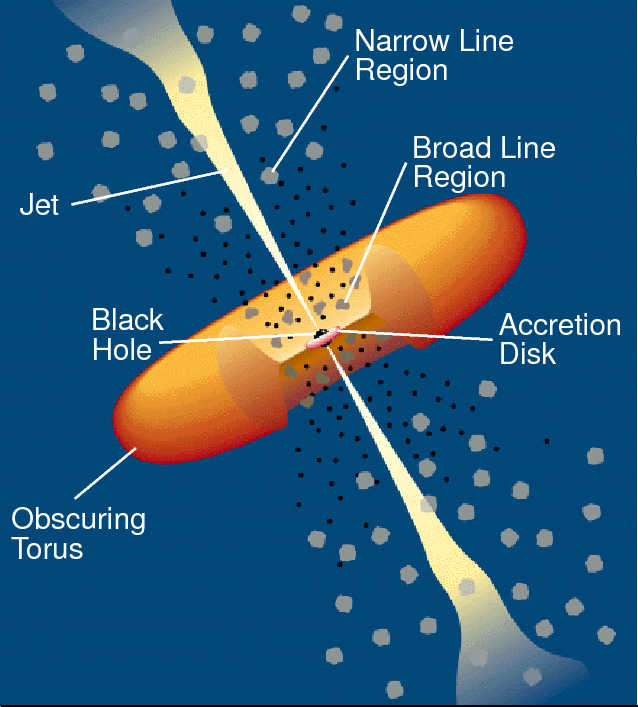
\includegraphics[width=0.5\textwidth]{figures/chapter06/urry_model}
  \caption{Illustration of the physical structure of an AGN in a simple orientation-based unification model. From \citet{urry95}.}
  \label{fig:agnmodel}
\end{figure}

AGNs are divided into numerous classes and sub-classes based on their observational properties. 
AGN unification models \citep{antonucci93,urry95} attempt to explain the diversity in their observational properties using as few physical parameters as possible. 
In many unification models the optical and radio luminosities are considered to be intrinsic parameters. Variations in the radio luminosity explains the difference between the $15-20\%$ of AGN which are {\it radio-loud} (i.e. have radio to optical flux ratios $\gtrsim$ 10) and the remainder which are {\it radio-quiet}. 
The optical luminosity explains, for example, the difference between low-luminosity {\it Seyfert Galaxies} and high-luminosity {\it quasars}\footnote{The term `quasar' is sometimes reserved for radio-loud objects and `quasi-stellar object', or `QSO', for radio-quiet objects. Here, `quasar' is used to refer to all luminous AGN.}.
In a typical quasar the optical emission may be brighter than the combined emission from all of the stars in the host galaxy by a factor of 100 or more. 
The large brightness contrast between the nucleus and the host galaxy makes the host galaxy difficult to detect, and the quasar is observed as an unresolved stellar-like object\footnote{The name `quasar' is shortened from `quasi-stellar radio source', since quasars were originally discovered as optical point-source counterparts to a newly discovered population of radio sources.}.   

Unification models attempt to explain all further observational differences as being apparent differences due to {\it orientation} effects. 
The basic physical structure of an AGN in this model is illustrated in Figure \ref{fig:agnmodel}. 
Material is pulled towards the SMBH at the centre and sheds angular momentum through viscous and turbulent processes in an accretion disk, which radiates primarily at ultraviolet (UV) to soft-X-ray wavelengths. 
Strong optical and UV emission lines are produced in photo-ionised gas clouds moving rapidly in close proximity to the SMBH. 
The doppler-broadened emission line widths imply gas cloud velocities of thousands of km s$^{-1}$ in this {\it broad-emission line}. 
Further out are dusty, molecular clouds, the geometry of which is often modelled as a torus co-planar with the accretion disk. 
Along some lines of sight from the observer to the accretion disk / broad line region the dusty torus obscures the UV/optical radiation. 
In this case, an observer would see a weak UV/optical continua and no broad emission lines and classify the AGN as being {\it Type II}. 
On the other hand, if the line of sight is unobscured by the dusty torus then a broad emission line component would be observable in the spectrum and the AGN would be classified as being {\it Type I}. 
Further away from the central black hole and beyond the dusty torus are slower moving clouds of gas which are photo-ionised by the continuum emission from the accretion disk and produce forbidden emission lines of narrower widths (typically hundreds of km s$^{-1}$). 
Outflows of energetic particles occur along the poles of the accretion disk and form collimated radio-emitting jets and in some cases giant radio-emitting lobes. 
A strong, relativistically beamed component with large variations in brightness on very short timescales (e.g. ${\Delta}m \gtrsim 0.1$ and $\Delta t \lesssim 1$ day) is observed and a source with these properties is classified as a {\it blazar}. 

While an orientation-based unification scheme such as this is somewhat successful at explaining many of the observational properties of AGNs, other factors such as the host galaxy morphology and gas/dust content may also be important \citep{peterson95}. 
It is also doubtful whether the geometry of the dusty torus is the same in all AGNs, and the fraction of obscured quasars has been shown to decrease with increasing nuclear luminosity \citep{lawrence91}. 
As we will now discuss, quasars might play an important role in a broader cosmological context, affecting the formation and evolution of the galaxies, groups, and clusters in which they reside. 
In this scenario of galaxy/quasar co-evolution the quasar is expected to transition from a highly active obscured phase to an unobscured phase as it clears out the dust surrounding it. 
If this picture is true then we should expect to find variations in the observational properties of the quasar and host galaxy as the system transitions through the different stages of its evolution.  

\section{The Torus}

Elitzur \& Shlosman (2006): 

Recent high-resolution IR observations indicate that the torus size might be no more than a few parsecs (Elitzur 2005 and references therein); in particular, VLTI observations of NGC 1068 show that the FWHM size of the 12 mm emission is only 4 pc (Jaffe et al. 2004). The compact sizes place the torus inside the region where the SBH gravity dominates over the galactic bulge.

Two approaches have been taken for the torus dynamic origin. A hydrostatic scenario depicts the torus as a doughnut-like structure populated by molecular clouds accreted from the galaxy (Krolik \& Begelman 1988). However, the origin of vertical mo tions capable of sustaining the clouds in a hydrostatic structure with H$\sim$R was recognized from the start as problematic and has eluded solution thus far (e.g., Davies et al. 2006). The other
scenario, based on the seminal work by Blandford \& Payne (1982), involves the outflow of clouds embedded in a hydromagnetic disk wind (Emmering et al. 1992, hereafter EBS92; Konigl \& Kartje 1994; Kartje \& Konigl 1996; Bottorff et al. 1997, 2000; Kartje at al. 1999; Everett 2005). In this approach the torus is merely a region in the wind that happens to provide the required toroidal obscuration; i.e., it is that region wherein the clouds are dusty and optically thick.



\section{Evolutionary Models}

A number of observations link the growth and evolution of quasars to the growth and evolution of galaxies. These include the following: 

\begin{enumerate}
\item SMBHs appear to be a ubiquitous feature at the centres of all massive galaxies \citep[e.g.][]{kormendy13}. 
\item SMBH masses are proportional to the mass/velocity dispersion of their host spheroid \citep[the $M-\sigma$ relation;][]{ferrarese00,gebhardt00}.
\item The cosmological evolution of the star formation rate and the quasar luminosity function are very similar \citep[e.g.][]{wall05}.
\item Cosmological simulations of galaxy formation and evolution require feedback from SMBH growth in order to reproduce the galaxy luminosity function \citep{kauffmann00}.
\end{enumerate}

These observations suggest that all galaxies may have gone through a `quasar phase' during which the SMBH accretes most of its mass and the stellar-bulge forms most of its stars. 
This evolutionary phase could be triggered by a major merger or by instabilities in the galactic disc or bulge. 
In a galaxy merger large amounts of gas can shed sufficient angular momentum to settle into dense clouds and form stars or be funnelled to the centre of the galaxy to grow the existing SMBH. 
The large amounts of gas and dust funnelled inward to the galactic nucleus is predicted to obscure the quasar until the dust is cleared out either by quasar-driven or stellar-driven processes. 
An un-obscured quasar then emerges, and is active until all of the available material has been accreted \citep{hopkins06a, narayanan10}. 
The feedback processes involved are also thought to be responsible for shutting down star formation in the galactic bulge \citep{silk98} and establishing the $M-\sigma$ relation. 

Such scenarios have been invoked to explain the presence of buried AGN seen in ultra-luminous infra-red galaxies \citep[ULIRGs;][]{sanders88}, a high fraction of which also show evidence of merging and interaction. 
However, the full picture is likely to be more complicated. Although there is evidence that mergers dominate at high luminosities \citep{treister12}, stochastic accretion may be more important at low luminosities \citep[e.g.][]{hopkins06b}. 

Luminous unreddened quasars show few signs of interaction \citep[e.g.][]{dunlop03} which, if the quasar-galaxy co-evolution model is true, suggests that indications of an interaction disappear during a transitional phase. Quasars in this transitional phase would be highly reddened, as the dust enshrouding the nucleus will not have been fully cleared, but not completely obscured. 
A population of quasars with these properties may therefore represent a link between ULIRGs and unobscured quasars. 

\section{Interesting Sub-Populations}

\subsection{Red and Reddened Quasars}

Magnitude limited optical surveys of quasars are biased against selecting red and reddened quasars. 
\citet{richards03} studied a large sample of optically selected Sloan Digital Sky Survey \citep[SDSS;][]{york00} quasars and showed the mean reddening to be $E(B-V) = 0.03$ at the redshift of the quasar. 
They estimated that $\sim 15\%$ of the population was missing from the survey due to dust extinction. 
The missing fraction, and it's dependence on luminosity and redshift, could help to determine whether the reddened population is best explained in the context of orientation-based unification models with non-spherical geometry or as an evolutionary stage in a quasars lifetime.   

Populations of heavily dust-reddened quasars have been identified using radio surveys \citep[e.g.][]{glikman12}, by using the `$K$-band excess' in the spectra of quasars relative to stars \citep{maddox12}, and using near-IR colour selection \citep{banerji12,banerji13}. 
Recently, \citet{ross14} identified a small sample of very red SDSS quasars based on their extreme IR to optical luminosity ratios. 
It is yet to be determined whether these extreme objects are simply the tail of a population dominated by less reddened quasars, or whether the distribution is bi-modal with reddening. 
A population of quasars with intermediate amounts of dust reddening ($0.1 \lesssim {\rm E(B-V)} \lesssim 0.5$) would help to address this question. 

\subsection{Broad Absorption Line Quasars}

{\it Broad absorption line quasars} (BALQSOs) are a sub-population of quasars exhibiting blue-shifted absorption troughs broader than 2000kms$^{-1}$ \citep{weymann91} which are unambiguously associated with AGN-driven out-flowing gas. 
As well as showing high rates of mergers, an anomalously large fraction of heavily reddened objects exhibit broad blue-shifted absorption troughs in their spectra \citep{urrutia09, glikman12}. 
This observation suggests that the BAL phenomenon may be related to a `blow-out' phase of a quasars lifetime as it transitions from a dusty, obscured objected to a luminous blue quasar, at the same time quenching star formation. Since outflows are believed to be fundamental to AGN feedback, a better understanding of their properties could shed light on the outflow phenomenon. 
Alternatively, whether a quasar is observed to have broad absorption lines could depend only on the orientation of the observer in relation to an intrinsically anisotropic system.

\subsection{Hot-Dust-Poor Quasars}

The near-IR emission from AGN is generally explained by thermal emission from dust grains at the edge of the dusty torus closest to the accretion disk. 
The dust is heated to its sublimation temperature \citep[1300-2000K][]{barvainis92} by emission from the accretion disc. However, \citet{hao10} reported that 6\% (at $z \lesssim 2$) to 20\% (at $2 \lesssim z \lesssim 3.5$) of the quasars in the X-ray selected XMM-COSMOS Type 1 AGN sample \citep{brusa10} have an unusually small amount of hot dust emission, despite having normal accretion disc spectra. 
They infer a torus covering factor of  $\sim$2\% to 30\% for these `hot dust poor' (HDP) quasars, well below the $\sim$75\% predicted by unified models \citep[e.g.][]{krolik88}. 
\citet{hao11} found that HDP quasars were just as common in the \citet{richards06} Spitzer/SDSS sample ($8.7\% \pm 2.2\%$) and the \citet{elvis94} Palomar-Green-quasar-dominated sample ($9.5\% \pm 5.0\%$). 
Either the hot dust is destroyed (dynamically or by radiation), or the dust is not centred on the SMBH, which could happen during a major merger \citep[e.g.][]{blecha11}. 
Alternatively, misaligned accretion disks, which will result from discrete isotropic accretion events \citep{volonteri07}, will lead to a wider range of covering factors \citep{lawrence10}. 

At higher redshifts, \citet{jiang10} found two HDP quasars in a sample of 21 at $z\sim6$. 
They find that at $z\sim6$ the hot dust abundance is roughly proportional to the black hole mass, indicating that the two grow at about the same rate. 
The two HDP quasars also have the smallest SMBH masses, and may be too young to have formed a significant amount of hot dust.

\subsection{Type II Quasars}

As well as lacking a broad-line spectral component, Type II AGN tend to have high IR to optical light ratios, hard X-ray spectra, and be strongly polarised, consistent with dusty torus based unification schemes. 
The detection of unobscured continuum emission that is scattered and polarised by dust above the torus has confirmed the orientation-based unification of Type I and Type II Seyfert Galaxies. 
Their higher luminosity analogues, Type II quasars, have been much more difficult to detect and study. 
It is possible that the orientation-based Type I/II unification scheme may break down at high-luminosities, and that instead all quasars could pass through a Type II phase before the obscuring dust is cleared out by the quasar-driven outflows and a Type I quasar emerges.  

\section{Spectral Energy Distributions}
\label{sec:sed}

\begin{figure}
  \centering
  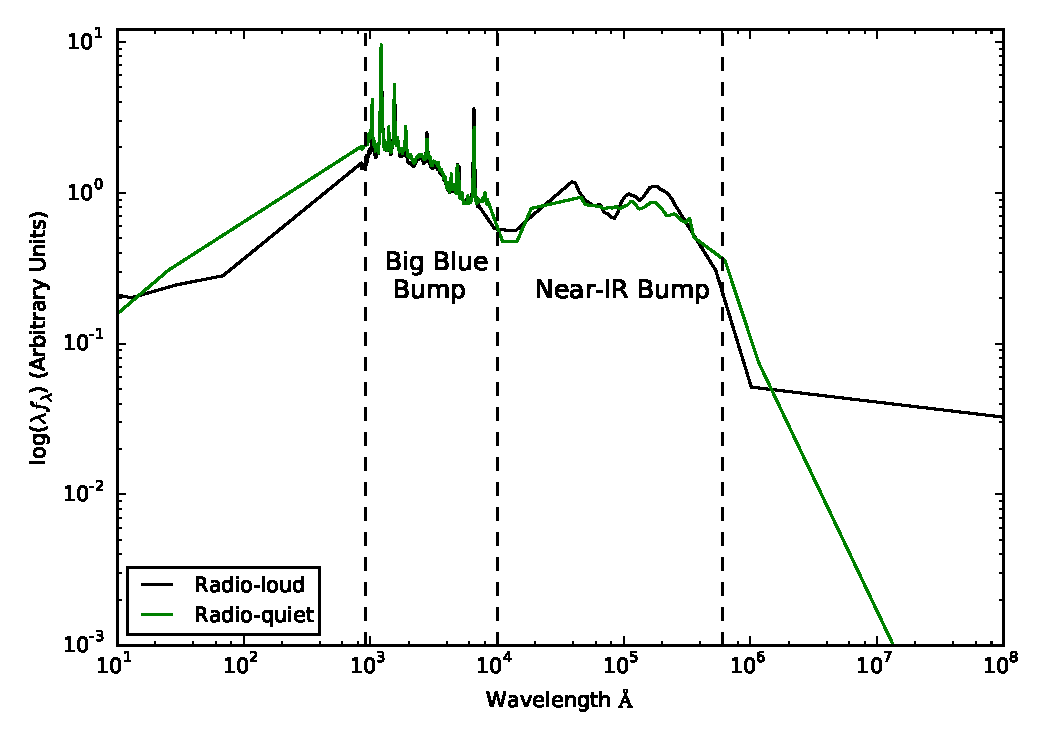
\includegraphics[width=\textwidth]{figures/chapter01/shangsed.pdf}
  \caption{Median SEDs for radio-loud and radio-quiet quasars from \citet{shang11}.}
  \label{fig:seyfert_sed}
\end{figure}

AGNs emit strongly over many decades in frequency of the electromagnetic spectrum and the energy emitted as a function of frequency is described by a {\it spectral energy distribution} (SED). 
As we will describe below, the broad features in the SED originate from processes which occur in different regions of the AGN. 
In the preceding sections, we have described how some interesting sub-populations of AGNs might relate to the broader population in the context of orientation-based unification schemes and evolutionary schemes. 
Comparing SEDs of different sub-populations can help to shed light on these relationships and the physical processes which drive them. 
Possible correlations between the SED shape and luminosity, redshift, and other properties of the AGN such as black hole mass and Eddington ratio can also constrain models of AGN structure and evolution. 

Since the physical processes involved are generally understood only qualitatively, almost all AGN SED templates are empirical. 
The empirical template of \citet{elvis94}, constructed using photometric observations from the radio to the hard X-rays of 29 radio-quiet and 18 radio-loud Type I quasars, is still the most commonly cited, despite many additions and updates \citep[e.g.][]{polletta00, kuraszkiewicz03, risaliti04, richards06,  polletta07, lusso10, shang11, marchese12, trichas12}. 
In Figure \ref{fig:seyfert_sed} we show the median spectrum from the radio-loud and radio-quiet samples of Shang et al. (2011). 
Short-ward of the radio region, the radio-loud and radio-quiet spectra are almost indistinguishable. 

A large amount of energy is emitted in the UV/optical region short-ward of $\sim4000$\AA: the {\it Big Blue Bump}. In the X-ray region, the {\it soft X-ray excess} may be the high-energy end of this feature. 
The Big Blue Bump is generally attributed to thermal emission from the accretion disk. 
In Type II AGNs, the continuum emission from the accretion disk is obscured, and so the Big Blue Bump in the SED of a Type II AGN would be less prominent than is seen in Figure \ref{fig:seyfert_sed}. 

The feature at wavelengths long-ward of $\sim1\mu$m is the {\it IR Bump}, and is generally attributed  to thermal emission from dust at a wide range of temperatures ($\sim50 - 1000$ K). 
The amount, geometry, ionisation and optical depth of absorbing dust and gas and its inclination determines the shape of the IR Bump and the absorption of the optical/UV continua. 
The relative strengths of the IR Bump and the Big Blue Bump are generally comparable, although they do vary from object to object. 
In particular, for the HDP objects we described above the IR Bump appears to be missing entirely. 
The minimum between the two peaks is at $\sim1\mu$m, which reflects the sublimation of dust at T $\gtrsim 2000$ K \citep{sanders89}.

Emission in the hard X-ray region of the spectrum is believed to be due to Compton up-scattering of accretion disk photons by hot electrons forming a corona in the vicinity of the disk \citep[e.g.][]{sunyaev80}. 
The radio emission, which originates from synchrotron emission in relativistic jets, contributes very little to the total energy output.
However, the mechanical energy provided by the jets is an important component of AGN feedback models \citep[e.g.][]{fabian12}. 

Many parameters might be expected to affect the shape of the AGN SED (e.g. the black hole mass, the accretion rate, the physical properties of the accretion disk, the properties of the absorbing dust) and many of these properties might be expected to change as the quasar evolves (e.g. as dust is expelled from the nuclear regions). Given this, it is perhaps surprising that many authors have found no significant dependence of the mean SED on properties such as redshift, bolometric luminosity, SMBH mass, or accretion rate \citep[e.g.][]{elvis12,hao13} and that quasars up to redshift 7 have been shown to have similar UV spectra to low redshift quasars \citep[e.g.][]{mortlock11}.

Throughout this thesis we adopt a $\Lambda$CDM cosmology with $h_0=0.71$, $\Omega_M=0.27$, and $\Omega_\Lambda=0.73$. 
All wavelengths and equivalent width measurements are given in the quasar rest-frame, and all emission line wavelengths are given as measured in vacuum.

Everett et al. (2005): 

A variety of observational signatures point to the importance of outflowing gas within many types of active galactic nuclei (AGNs). Blueshifted absorption features (in broad absorption line quasars, or BALQSOs; see, e.g., Weymann et al. 1991) are seen in approximately 15\% (Reichard et al. 2003) of radio-quiet quasars, with velocities up to 0.1c. In addition, radio-loud quasars display relativistic, collimated outflows. 
There has also been observational evidence that suggests the mass outflow rate in AGNs is nearly equal to the mass inflow rate (see, e.g., Crenshaw et al. 2003; Chartas et al. 2003).

% !TEX root = ../main.tex

%*****************************************
\chapter{A near-infrared spectroscopic database of high-redshift quasars}
\label{ch:nirsample}
%*****************************************

\section{Introduction}

Emission-lines provide a wealth of information about the properties of AGNs and their environments. 
They provide diagnostics of dynamics, temperatures, densities, dust content, elemental abundances and the shape of the ionising spectrum which are often unattainable through any other technique. 
The optical region includes a number of strong emission features, including the broad Balmer lines \ha ($6565$\,\AA) and \hb ($4863$\,\AA) and the narrow [\ion{O}{III}]$\lambda\lambda$$4960$,$5008$ doublet.
As we will see in Chapter~\ref{ch:bhmass}, the Balmer lines are routinely used to derive BH masses and AGN accretion rates. 
As the strongest narrow emission-line in the optical spectrum, [\ion{O}{III}] is used to measure systemic redshifts, and to probe AGN-driven outflows in the NLR (see Chapter~\ref{ch:nlr}). 

Large optical surveys have provided spectra for hundreds of thousands of AGN and quasars. 
With it's twelfth data release in $2016$, the number of AGNs and quasars in the Sloan Digital Sky Survey \citep[SDSS;][]{york00} spectroscopic catalogue alone reached almost $400\,000$. 
However, the rest-frame optical region is redshifted beyond the reach of optical spectrographs at redshifts $z \gtrsim0.4$. 
Accessing the rest-frame optical lines at redshifts $2 \lesssim z \lesssim 4$, during the peak epoch of galaxy evolution, requires near-infrared spectroscopy.  

Spectroscopic observations are more challenging at near-infrared wavelengths than in the optical because the Earth's atmosphere is both bright and highly variable at infrared wavelengths. 
As a result, the number of high-redshift quasars with near-infrared spectra is limited and previous investigations of the rest-frame optical spectra of quasars at redshifts $z\sim2$ have typically used samples containing a few dozen objects \citep[e.g.][]{marziani09,shen12,shen16a}. 

In this Chapter, I will describe the construction of a database containing $434$ high-redshift quasars. 
In later Chapters, I will describe how I have used this data to significantly reduce large systematic biases afflicting BH mass estimates for quasars at redshifts $z \gtrsim 2$ (Chapter~\ref{ch:bhmass}) and to study the prevalence and drivers of quasar-driven galaxy-wide outflows (Chapter~\ref{ch:nlr}). 
The unprecedented size and quality of this dataset make a number of other investigations possible, some of which are described in Chapter~\ref{ch:conclusions}. 

\section{Data}

\begin{table}
  \footnotesize
  \centering
  \caption{Summary of near-infrared spectroscopic database.}
  \label{tab:data_summary}
    \begin{tabular}{cc} 
    \hline
    Instrument & Number \\  
    \hline
    FIRE/Magellan   & $36$ \\
    GNIRS/Gemini    & $29$ \\
    ISAAC/VLT       & $13$  \\
    LIRIS/WHT       & $21$  \\
    NIRI/Gemini     & $31$ \\
    NIRSPEC/Keck    & $3$   \\ 
    SINFONI/VLT     & $84$ \\
    SofI/NTT        & $111$ \\
    TRIPLESPEC/ARC  & $38$ \\
    TRIPLESPEC/Hale & $60$ \\
    XSHOOTER/VLT    & $36$  \\
    \hline
    Total & $462$ \\
    \hline
    \end{tabular}
\end{table}

The near-infrared spectra in our database are taken from published catalogues, by downloading and reducing
archival spectra, and by reducing previously un-published spectra acquired in programmes led by Prof. J. Hennawi (UCSB) and Prof. X. Prochaska (UCO/LICK). 
As the P.I.\footnote{P.I.: Principle Investigator.} of two programmes, I targeted quasars with the goal of filling in under-sampled regions of the \ion{C}{IV} EQW and blueshift parameter space (see Section XX for a detailed discussion of \ion{C}{IV} emission properties in high-redshift quasars).
The telescopes and instruments used to observe the spectra are summarised in Table~\ref{tab:data_summary} and information on individual spectra is provided in Table~\ref{tab:database}.
There are $434$ unique quasars in our catalogue. 
Multiple spectra exists for a number of quasars, and the total number of spectra in our catalogue is $462$. 
The columns in Table~\ref{tab:database} are as follows: 

\begin{itemize}

\item[1] ID: Jhhmmss+ddmmss. ID is repeated when multiple spectra exist for the same object. 

\item[2] Unique catalogue name.   

\item[3] Date spectrum acquired. 

\item[4-5] RA and DEC (J$2000$; truncated coordinates).  

\item[6] Instrument and telescope used to acquire spectrum. 

\item[7] Wavelength range covered by spectrum. 

\item[8] Velocity per pixel in spectrum. 

\item[9] S/N per pixel in spectrum. 

\item[10] Redshift. 

\end{itemize}

\begin{landscape}% Landscape page
    \centering % Center table
    \begin{minipage}{\linewidth}
    \footnotesize
    \renewcommand\footnoterule{}
    \captionof{table}{Quasars in our near-infrared spectroscopic database. Only the first $15$ entries are shown. The full table (including $462$ objects) is available on-line. \todoinline{Maybe DVD? Ask Debbie}}
    \label{tab:database}
    \begin{tabular}{cccccccccc} 
    \toprule
     ID &   Cat. Name &  Date &             Ra &            Dec &            Instr. &  $\Delta\lambda$ [$\mu$m] &  $\Delta v$ [\kms] & S/N &  $z$ \\
     ($1$) &        ($2$) &             ($3$) &            ($4$) &            ($5$) &  ($6$) &  ($7$) & ($8$) &  ($9$) & ($10$) \\
    \midrule
    J$000039$-$001804$  &  QSO$460$ & $2015$-$09$-$02$ &  +$00$h$00$m$39$.$00$s &  -$00$d$18$m$03$.$90$s &         SofI/NTT &  $1.50$-$2.54$ &     $154.0$ &   $4.9$ &  $2.14$ \\
    J$000345$-$232353$  &  QSO$552$ & $2009$-$07$-$07$ &  +$00$h$03$m$45$.$00$s &  -$23$d$23$m$53$.$40$s &      SINFONI/VLT &  $1.44$-$1.87$ &      $36.0$ &  $12.7$ &  $2.27$ \\
    J$000345$-$232353$  &  QSO$330$ & $2011$-$09$-$18$ &  +$00$h$03$m$45$.$00$s &  -$23$d$23$m$53$.$40$s &         SofI/NTT &  $1.48$-$1.83$ &      $63.0$ &  $36.0$ &  $2.26$ \\
    J$000451$-$084450$  &  QSO$290$ & $2013$-$07$-$12$ &  +$00$h$04$m$50$.$66$s &  -$08$d$44$m$49$.$63$s &     XSHOOTER/VLT &  $0.31$-$2.28$ &      $15.0$ &  $10.3$ &  $3.00$ \\
    J$000451$-$084452$  &  QSO$289$ & $2013$-$08$-$08$ &  +$00$h$04$m$50$.$91$s &  -$08$d$44$m$51$.$98$s &     XSHOOTER/VLT &  $0.31$-$2.28$ &      $15.0$ &   $5.4$ &  $3.00$ \\
    J$000500$-$003348$  &  QSO$454$ & $2015$-$09$-$01$ &  +$00$h$05$m$00$.$42$s &  -$00$d$33$m$48$.$20$s &         SofI/NTT &  $1.50$-$2.54$ &     $154.0$ &   $8.2$ &  $2.18$ \\
    J$000501$+$010221$  &  QSO$459$ & $2015$-$09$-$02$ &  +$00$h$05$m$00$.$53$s &  +$01$d$02$m$20$.$80$s &         SofI/NTT &  $1.50$-$2.54$ &     $154.0$ &   $6.8$ &  $2.13$ \\
    J$001016$+$001228$  &  QSO$475$ & $2015$-$09$-$04$ &  +$00$h$10$m$16$.$49$s &  +$00$d$12$m$27$.$60$s &         SofI/NTT &  $1.50$-$2.54$ &     $154.0$ &   $8.9$ &  $2.28$ \\
    J$001247$+$001239$  &  QSO$082$ & $2013$-$06$-$06$ &  +$00$h$12$m$47$.$12$s &  +$00$d$12$m$39$.$49$s &        ISAAC/VLT &  $1.52$-$1.60$ &      $15.0$ &  $19.1$ &  $2.16$ \\
    J$001708$+$813508$  &  QSO$107$ & $2012$-$08$-$04$ &  +$00$h$17$m$08$.$48$s &  +$81$d$35$m$08$.$10$s &  TRIPLESPEC/Hale &  $0.94$-$2.80$ &      $39.0$ &  $36.5$ &  $3.40$ \\
    J$001919$+$010152$  &  QSO$476$ & $2015$-$09$-$04$ &  +$00$h$19$m$19$.$31$s &  +$01$d$01$m$52$.$20$s &         SofI/NTT &  $1.50$-$2.54$ &     $154.0$ &   $6.5$ &  $2.32$ \\
    J$001955$-$091316$  &  QSO$001$ & $2004$-$11$-$26$ &  +$00$h$19$m$54$.$67$s &  -$09$d$13$m$16$.$45$s &     GNIRS/Gemini &  $0.60$-$2.61$ &      $88.0$ &   $9.9$ &  $2.12$ \\
    J$002018$-$233654$  &  QSO$553$ & $2009$-$07$-$07$ &  +$00$h$20$m$18$.$41$s &  -$23$d$36$m$53$.$80$s &      SINFONI/VLT &  $1.44$-$1.87$ &      $36.0$ &  $16.9$ &  $2.30$ \\
    J$002023$-$414639$  &  QSO$554$ & $2009$-$07$-$08$ &  +$00$h$20$m$23$.$38$s &  -$41$d$46$m$38$.$90$s &      SINFONI/VLT &  $1.09$-$1.41$ &      $35.0$ &  $33.4$ &  $1.57$ \\
    J$002111$-$242247$  &  QSO$555$ & $2009$-$07$-$16$ &  +$00$h$21$m$10$.$90$s &  -$24$d$22$m$47$.$20$s &      SINFONI/VLT &  $1.44$-$1.86$ &      $36.0$ &  $11.1$ &  $2.26$ \\
    \bottomrule
    \end{tabular}
    \end{minipage}
\end{landscape}

\subsection{\citet{coatman16} Quasars}

\subsubsection{Target selection}

We selected quasars from the Seventh Data Release \citep[DR7;][]{schneider10} of the SDSS spectroscopic quasar catalogue.  
The sample was restricted to objects with redshifts $2.14 < z <2.51$ ($7,258$ quasars), to ensure that the \hb and \ha emission-lines fall within the $H$- and $K$-passbands respectively, allowing us to observe both simultaneously with the appropriate grism configuration.
Given the limited number of quasars for which near-infrared spectra could be obtained, the quasar sample was further restricted to objects that are radio-quiet ($5,980$ quasars), show no evidence of broad absorption-lines (BALs) in their spectra ($5,299$ quasars), and are free from significant dust extinction. 
We removed radio-loud objects and BAL quasars using the classification flags described in Section~\ref{sec:ch2-flags}. 
The removal of quasars with significant dust extinction was achieved by identifying quasars with $i-K$ colours redder than a parametric spectral energy distributions (SED) model combined with an extinction curve with \ebv=$0.05$ (a very similar procedure is described in greater detail in Section~\ref{sec:ch5-hotdustsample}). 

The $K$-magnitude (used to compute the $i-K$ colour) was taken from the UKIRT Infrared Deep Sky Survey \citep[UKIDSS;][]{lawrence07} Large Area Survey (ULAS). 
The requirement to be in the ULAS footprint and have reliable $K$ passband photometry reduced our sample of possible targets to $1,683$, and the \ebv\, cut left $1,204$ in our sample. 
Finally, a flux-limit of $K<18.5$ (AB) was applied to ensure that spectra of sufficient signal-to-noise ratio (S/N) could be obtained (leaving $412$ quasars). 
 
We were able to obtain new infrared spectra for $19$ quasars from this sample of $412$ possible targets. 
The quasars included in this sub-sample were selected to have \ion{C}{IV}-emission shapes which span the full range observed in the population. 
Reliably quantifying the distribution of \ion{C}{IV}-emission shapes has been made possible thanks to recent improvements in the estimation of systemic redshifts from ultra-violet spectra (see Section~\ref{sec:ch3-recipe} for details). 

\subsubsection{Observations}

Near-infrared spectra were obtained with the Long-slit Intermediate Resolution Infrared Spectrograph \citep[LIRIS;][]{manchado98} mounted on the $4.2$\,m William Herschel Telescope (WHT) at the Observatorio del Roque de los Muchachos (La Palma, Spain). 
Observations took place over four non-contiguous nights from $2015$ March $31$ to April $4$. 
Approximately one night was lost due to poor weather and a further half-night was affected by poor transparency due to cloud. 
A one\,arcsecond slit-width was employed and the LIRIS $H+K$ low-resolution grism was selected, which covers the spectral ranges $1.53-1.79$\,$\mu$m and $2.07-2.44$\,$\mu$m with a dispersion of $9.7$\,\AA/pixel. 
The spatial scale of the instrument is $0.25$\,arcsecond/pixel. 
Observations were divided into $60$\,second sub-exposures and performed in an ABBA nodding pattern, with the object placed at two positions along the slit $12$\,arcsecond apart. 
Bright A$0-5$V stars were observed at similar air-masses to the targets in order to provide both telluric absorption corrections and a flux calibration of the quasar spectra.

\subsubsection{Data reduction}

The raw LIRIS data frames incorporate a known `pixel shift' which was first removed from all frames using the LIRIS data reduction package {\tt LIRISDR}. 
Subsequent data reduction was undertaken with standard {\tt IRAF}\footnote{IRAF is distributed by the National Optical Astronomy Observatory, which is operated by the Association of Universities for Research in Astronomy (AURA) under a cooperative agreement with the National Science Foundation.} procedures\footnote{The data reduction pipeline is available at https://github.com/liamcoatman/SpectraTools.}.  
The flat-field images, which were taken at the beginning of each night via illumination of the dome, were averaged and normalised to remove any wavelength-dependent signature. 
Each individual two-dimensional spectrum was then flat-field corrected. 
Consecutive AB and BA pairs of two-dimensional spectra were subtracted to remove the sky background. 
All the subtracted AB/BA-pairs for a given target were then averaged to give the final two-dimensional spectrum.

The size of the one-dimensional spectrum extraction windows, in the slit direction, varied from $6-10$ pixels. 
To increase the S/N, optimal variance-weighted extraction with sigma clipping was employed. 
For the fainter objects in our sample we were unable to trace the spectrum across the dispersion axis reliably and the trace from a telluric standard-star observation, observed at a similar air mass and time, was used instead. 
The wavelength calibration, using argon and xenon lamp exposures, resulted in root mean square errors in the range $1.01-1.71$\,\AA, with a mean of $1.47$\,\AA. 
The telluric standard star observations were reduced using the same steps described above. 
The stellar continuum was divided out of the standard star spectrum, which was then divided into the quasar spectrum to remove telluric absorption features. 
The spectral type and magnitude of the standard star were used to flux calibrate the quasar spectrum both in a relative and absolute sense.

\subsection{\citet{shen12} and \citet{shen16a} quasars}

\citet{shen16a} and \citet{shen12} obtained near-infrared spectroscopy for a sample of $74$ luminous, $1.5 < z < 3.5$ quasars selected from the SDSS DR$7$ quasar catalogue. 
Targets were required to possess good optical spectra covering the \ion{C}{IV} line and have redshifts $z\sim$ $1.5$, $2.1$, and $3.3$ to ensure that the \hbns-[\ion{O}{iii}] region was covered in one of the near-infrared $JHK$ passbands.
Thirty-eight of the quasars were observed with TripleSpec \citep{wilson04} on the Astrophysics Research Consortium (ARC) $3.5$\,m telescope, and $36$ with the Folded-port InfraRed Echellette \citep[FIRE;][]{simcoe10} on the $6.5$\,m Magellan-Baade telescope.
The reduction of the spectra is described in \citet{shen16a} and \citet{shen12}. 

\subsection{Quasar pairs}

A large part of our catalogue was observed as part of an ongoing effort to identify quasar pairs at very close projected separations \citep[Quasars Probing Quasars\footnote{www.ucolick.org/\textasciitilde xavier/QPQ/Quasars\_Probing\_Quasars};][]{hennawi06a,hennawi10}. 
The primary science driver of this work is to study the circum-galactic medium of the foreground quasars in absorption \citep{hennawi06b}.
Very accurate systemic redshift measurements are a requirement and a large amount of resources have been devoted to obtaining near-infrared spectra which cover low-ionisation broad lines or features from the quasar NLR \citep{prochaska09,lau16,hennawi15}. 

Twenty-nine quasars were observed with the Gemini Near-Infrared Spectrograph \citep[GNIRS;][]{elias06} on the 8.1 m Gemini North telescope, thirteen using the Infrared Spectrometer And Array Camera \citep[ISAAC;][]{moorwood98b} on the European Southern Observatory (ESO) Very Large Telescope (VLT), thirty-one with the Near InfraRed Imager and Spectrometer \citep[NIRI;][]{hodapp03} also on Gemini North and thirty-six with XSHOOTER \citep{vernet11}, again, on the VLT. 

The  XSHOOTER  spectra  were  reduced  with  a  custom  software  package  developed  by  George  Becker \citep[for details, see][]{lau16}. 
The remaining data was processed with algorithms in the LowRedux\footnote{www.ucolick.org/\textasciitilde xavier/LowRedux} package \citep[see][]{prochaska09}.

\subsection{VLT SINFONI quasars}

We performed a search of the ESO archive for high-redshift quasars observed with the SINFONI  integral  field  spectrograph \citep{eisenhauer03,bonnet04} at VLT/UT$4$.
We found $79$ quasars with redshifts $1.5 < z < 3.7$ which have $H$ and/or $K$ SINFONI spectroscopy, covering the \hb and \ha lines respectively. 
Seventy-two of the quasars are from a large programme led by L. Wisotzki (programme $083$.B-$0456$(A)) to study the mass function and Eddington ratios of active BHs drawn from the Hamburg-ESO survey \citep{wisotzki00}.
A further seven SINFONI spectra are from a programme led by  J. D. Kurk (programme $090$.B-$0674$(B)) to obtain reliable BH mass estimates from \hans/\hb for a sample of radio-loud/radio-quiet SDSS quasars.

I reduced the SINFONI spectra using the package EASYSINF\footnote{www.mrao.cam.ac.uk/\textasciitilde rw$480$/easysinf}.  
The package, which is based on the ESO-SINFONI pipeline, is described in \citet{williams16}. 

\subsection{ESO NTT SOFI quasars}

One quarter of the quasar catalogue derives from a large programme (programme $187$.A-$0645$; PI: J. Hennawi) to combine near-infrared spectra from SOFI \citep{moorwood98a} on the $3.6$\,m New Technology Telescope (NTT) with archival high-resolution optical spectra from the UV-Visual Echelle Spectrograph \citep[UVES;][]{dekker00} at VLT/UT$2$ and the High Resolution Echelle Spectrometer \citep[HIRES;][]{vogt94} at Keck to construct a legacy database of bright, high-redshift ($2 < z < 4$) quasars with both rest-frame optical spectra, covering the \hbns-[\ion{O}{III}] complex, and high-resolution rest-frame ultra-violet spectra.
The main science goal is to obtain precise systemic redshifts which are crucial for the study of absorption-line systems.  
Observations were undertaken over $16$ nights from $2011$ September $2013$ to March.
I reduced these spectra using a custom pipeline using algorithms in the LowRedux package.

Over five nights from $2015$ August $31$ to September $4$ we obtained near-infrared SOFI spectra for a further $26$ quasars (programme $095$.B-$0644$(A); PI: L. Coatman). 
These quasars were selected from the SDSS DR$7$ quasar catalogue using criteria very similar to those described above for the WHT sample. 
In particular, we selected quasars with large \ion{C}{IV} blueshifts to improve the statistics in this region of the \ion{C}{IV} emission-line parameter space. 
The spectra were reduced using the same LowRedux pipeline described above. 

\subsection{Hale TripleSpec quasars}

A further $60$ quasars in our catalogue are bright SDSS quasars which were observed with the TRIPLESPEC spectrograph \citep{herter08} on the Palomar $200$-inch Hale telescope (P$200$). 
The objects were observed with the same science goals as the SOFI NTT large programme. 
The spectra were reduced using a custom pipeline, again using algorithms in the LowRedux package. 

\section{Redshift and luminosity distribution of catalogue}

\begin{figure}[h!]
    \centering
    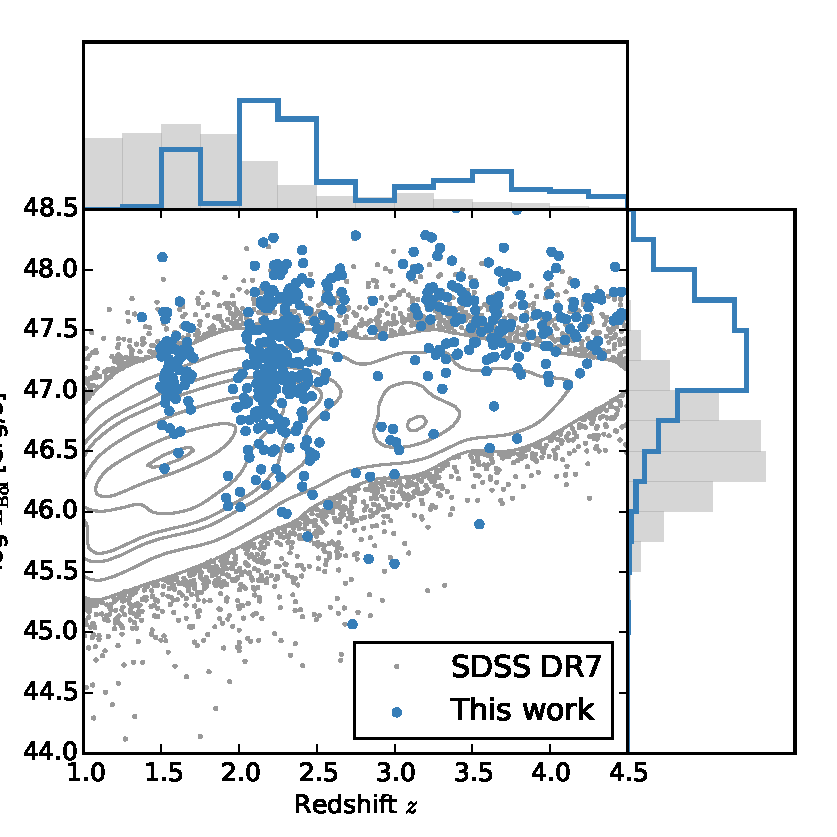
\includegraphics[width=0.8\textwidth]{figures/chapter02/luminosity_z.pdf} 
    \caption[{The ranges in redshift and luminosity covered by our sample, relative to the redshift-luminosity distribution of the SDSS DR$7$ quasar catalogue.}]{The ranges in redshift and luminosity covered by our sample, relative to the redshift-luminosity distribution of the SDSS DR$7$ quasar catalogue. For the SDSS sample we use \citet{hewett10} redshifts and bolometric luminosities measured by \citet{shen11}. For the quasars in this work the redshift is defined using the peak of the \hans/\hb emission and the luminosity is measured in the continuum at $1350$\,\AA\, and converted to a bolometric quantity using the same conversion factor employed by \citet{shen11}.}     
    \label{fig:lzplane}
\end{figure}

In Figure~\ref{fig:lzplane} we show the luminosities and redshifts of the quasar sample relative to the redshift-luminosity distribution for the Seventh Data Release \citep[DR$7$;][]{schneider10} of the SDSS spectroscopic quasar catalogue.
Our sample spans a redshift range $1.5 < z < 4.0$ and a bolometric luminosity range $10^{45.5}-10^{48}$\,\ergs. 
Spectra were obtained within one or more of the $JHK$ passbands and the gaps in our sample coverage at $z\sim1.8$ and $z\sim3$ are due to the presence of atmospheric absorption. 
Obtaining near-infrared spectra of adequate resolution and S/N of even moderately bright quasars remains resource intensive. 
As a consequence, at fixed redshift, the luminosities of the quasars are brighter than the average luminosity of the SDSS sample, although the dynamic range in luminosity is a full $1.5$ decades.

\section{Supplementary data}

\begin{table}
  \centering
  \footnotesize 
  \caption{Percentage of catalogue for which optical spectroscopic data is available from the given sources.}
  \label{tab:optical-data}
    \begin{tabular}{ccc}
    \hline
    & Source & \% \\
    \hline
    ($1$) & SDSS & $60$ \\
    ($2$) & BOSS & $45$ \\
    ($3$) & HAMBURG-ESO & $7$ \\
    ($4$) & VLT/UVES & $4$ \\
    ($5$) & VLT/XSHOOTER & $8$ \\ 
    \hline
    \end{tabular}
\end{table} 

\subsection{Optical spectroscopic data}

Optical spectra are available for $79$ per cent of the catalogue. 
The origin of these spectra is summarised in Table~\ref{tab:optical-data}. 
The sources of the optical spectra employed are as follows:

\begin{enumerate}

 \item The Seventh Data Release \citep[DR$7$;][]{schneider10} of the SDSS spectroscopic quasar catalogue. Spectra are moderate resolution ($R\simeq2000$) and S/N (S/N$\simeq20$) and cover the observed-frame wavelength interval $\sim3800-9180$\,\AA.   
 
 \item The Twelfth Data Release \citep[DR$12$;][]{paris17} of the Sloan Digital Sky Survey-III: Baryon Oscillation Spectroscopic Survey \citep[SDSS-III/BOSS;][]{dawson13}. Compared to SDSS spectra, BOSS spectra cover a slightly broader wavelength range and are typically higher S/N. 

 \item The Hamburg-ESO survey \citep{wisotzki00}. The spectra have a typical $R\simeq700$ spectral resolution and S/N $\gtrsim10$ per pixel. 

 \item Spectra taken with VLT/UVES. The reduced and fluxed UVES spectra were made available to us by A. Dall'Aglio (a description of the reduction procedure is contained in \citealt{dallaglio08}). The spectral resolution of the UVES observations is very high ($R\sim40\,000$) and the S/N of the spectra, re-binned to a resolution of $\simeq2000$, is S/N$\simeq300$. 

 \item Spectra taken with VLT/XSHOOTER. The XSHOOTER spectra are moderate resolution (R$\simeq6000$) and cover the full optical-near-infrared spectral region ($0.30-2.50$\,$\mu$m). 

\end{enumerate}

\subsection{Photometric data}

We cross-matched our catalogue with photometric data from the sources given below. 
The matching was done using a $5$ arcsecond matching radius, with only the closest neighbour retained in the case of multiple matches. 
The cross-matched surveys and the percentage of successful matches is summarised in Table~\ref{tab:cross-matching}. 
The columns in Table~\ref{tab:cross-matching} are as follows:

\begin{enumerate}

 \item SDSS DR$9$ photometric source catalogue. Point spread function magnitudes. 

 \item Two Micron All Sky Survey \citep[$2$MASS;][]{skrutskie06} Point Source Catalogue. Default magnitudes.

 \item UKIRT Infrared Deep Sky Survey \citep[UKIDSS;][]{lawrence07} Large Area Survey (DR$10$). $1$ arcsecond aperture corrected magnitudes (`apermag3').   

 \item Visible and Infrared Survey Telescope for Astronomy (VISTA) Hemisphere Survey \citep[VHS;][]{mcmahon13}. $1$ arcsecond aperture corrected magnitudes (`apermag$3$').   

 \item Kilo-Degree Infrared Galaxy \citep[VIKING;][]{edge13} Survey (DR$4$). $1$ arcsecond aperture corrected magnitudes (`apermag$3$').

 \item Wide-field Infrared Explorer \citep[WISE;][]{wright10} AllWISE Data Release \citep{mainzer11}. Profile-fitting magnitudes (`mpro').

\end{enumerate}

\subsection{Radio/BALQSO classification}
\label{sec:ch2-flags}

Using the catalogues provided by \citet{shen11}, \citet{allen11} and \citet{paris17} and visual inspection, 19 quasars in the catalogue are identified as being \ion{C}{IV} BALQSOs.  

We cross-match our catalogue to the FIRST radio catalogue \citep{white97}. 
We classify quasars with matches within $5$\,arcsecond as core-dominated, while, if multiple matches are found within $30$\,arcsecond, quasars are classified as lobe-dominated \citep[e.g.][]{shen11}. 
$128$ objects are outside of the FIRST footprint, $269$ are not detected in FIRST, $29$ are detected and are core-dominated, and $8$ are detected and are lobe-dominated. 

\begin{table}
  \centering
  \footnotesize 
  \caption{Cross-matched surveys and the percentage of successful matches.}
  \label{tab:cross-matching}
    \begin{tabular}{ccccccc} 
    \hline
     & SDSS & $2$MASS & UKIDSS & VHS & VIKING & WISE \\
     & ($1$) & ($2$) & ($3$) & ($4$) & ($5$) & ($6$) \\ 
    \hline
    $u$ & $73$ & - & - & - & - & - \\
    $g$ & $73$ & - & - & - & - & - \\
    $r$ & $73$ & - & - & - & - & - \\
    $i$ & $73$ & - &  & - & - & - \\
    $z$ & $73$ & - & - & - & $9$ & - \\
    $Y$ & - &  & $41$ & $10$ & 9 & - \\
    $J$ & - & $57$ & $41$ & $34$ & $9$ & - \\
    $H$ & - & $57$ & $41$ & $20$ & $9$ & - \\
    $K$ & - & $57$ & $41$ & $33$ & $9$ & - \\
    $W1$ & - & - & - & - & - & $97$ \\
    $W2$ & - & - & - & - & - & $97$ \\
    $W3$ & - & - & - & - & - & $97$ \\
    $W4$ & - & - & - & - & - & $97$ \\
    \hline
    \end{tabular}
\end{table} 

\section{Absolute flux calibration of near-infrared spectra}

Relative flux-calibration of the infrared spectra as a function of wavelength has been achieved through observations of appropriate flux standards. 
The absolute flux levels, however, can be in error by large factors due to variable atmospheric conditions combined with the narrow slit widths. 
For the majority of the quasars we have, therefore, established the absolute flux scale for each near-infrared spectrum using either the SDSS/BOSS spectroscopy or the available photometric data.

When an SDSS spectrum is available, we leverage the excellent flux calibration of these spectra to calibrate the near-infrared spectra. 
If a BOSS spectrum available, and an SDSS is not, then this is used instead. 
We use the quasar SED model described in Chapter~\ref{ch:sed} to bridge the gap between the wavelength coverage of the near-infrared and optical SDSS/BOSS spectra.
The SED model, described in Chapter~\ref{ch:sed}, gives a very good fit to the SDSS and UKIDSS magnitudes of SDSS DR$7$ quasars, reproducing the individual magnitudes with a $\sigma <0.1$\,mag.
The first step is to fit this quasar SED model to the SDSS/BOSS spectrum. 
The fit was done using a simple variance-weighted $\chi^2$ minimisation procedure in several emission-line-free intervals of the optical spectra.   
To avoid the known issues in the flux calibration of the BOSS DR$12$ quasar spectra at observed-frame blue wavelengths \citep{lee13}, our fitting was confined to rest-frame wavelengths long-ward of $1275$\,\AA. 
The second step is to fit the near-infrared spectrum to the normalised SED model. 
Regions of the spectrum which fall between the near-infrared transmission passbands are masked-out in the fitting procedure. 
The flux calibration method is demonstrated in Figure~\ref{fig:normalise_to_sdss_a}. 

\begin{figure}
    \captionsetup[subfigure]{labelformat=empty}
    \centering
    \subfloat[\label{fig:normalise_to_sdss_a}]{}
    \subfloat[\label{fig:normalise_to_sdss_b}]{}    
    \subfloat[]{{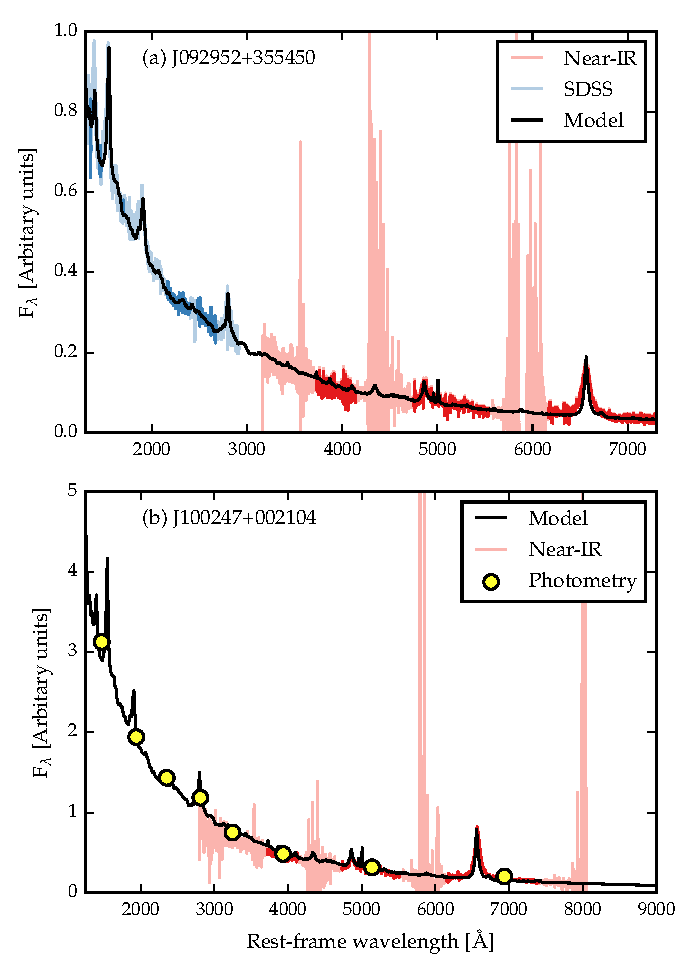
\includegraphics[width=\textwidth]{figures/chapter02/normalise_to_sdss.pdf} }}
    \caption[{}]{Demonstration of how the absolute flux calibration of the near-infrared spectrum (shown in red) is established using the SDSS spectrum (shown in blue, a) and photometric data (b). An empirical quasar SED model (shown in black) is used to bridge the discontinuity in the wavelength coverage of the optical/near-infrared spectroscopic and photometric data. The darker regions of the spectra are used in the fitting procedures.}     
    \label{fig:normalise_to_sdss}
\end{figure}

If an SDSS/BOSS spectrum is unavailable, then a second flux calibration method is adopted. 
This method is identical, except that the SED model is first fit to the available optical (SDSS) and near-infrared (VHS, Viking, UKIDSS or $2$MASS) photometric data. 
The SED model was integrated through the passband transmission functions, to give model magnitudes, and a variance weighted least-squares fit was done to the observed magnitudes. 
This procedure is illustrated in Figure~\ref{fig:normalise_to_sdss_b}. 

We are unable to verify the absolute flux calibration of the near-infrared spectra for four objects because neither SDSS/BOSS spectra nor optical/near-infrared data is available. 
The methods used to flux calibrate the near-infrared spectra are summarised in Table~\ref{tab:flux_calibration}. 

\begin{table}
  \centering
  \footnotesize 
  \caption{Methods used in absolute flux calibration of near-infrared spectra.}
  \label{tab:flux_calibration}
    \begin{tabular}{cc} 
    \hline
    Method & \% \\
    \hline
    SDSS               & $60$ \\
    BOSS               & $9$ \\
    NIR photometry     & $25$ \\
    NIR+OPT photometry & $6$ \\
    None               & $1$ \\    
    \hline
    \end{tabular}
\end{table} 

\todo{Ask Manda: (1+z) in luminosity calculation.}
The flux at $1350$ and $5100$\,\AA\, was read off directly from the normalised SED model.
These values were used to compute monochromatic continuum luminosities at $1350$ and $5100$\,\AA, which we use to estimate BH masses and bolometric luminosities in Chapters 3-5. 
Comparison of the $5100$\,\AA\, luminosity, computed using the photometry- and spectrum-based methods for $296$ quasars, showed a scatter (mean absolute deviation) of just $\sim0.1$\,dex.
We therefore assume $0.1$\,dex to be the measurement uncertainty on the $5100$\,\AA\, luminosities.
We expect the uncertainties on the $1350$\,\AA\, luminosities to be at similar level.  
For all the catalogue quasars, the optical and near-infrared spectra as well as the near-infrared photometry were obtained at different epochs, with rest-frame time differences of up to $\sim5$ years. 
Intrinsic quasar photometric variability in the rest-frame ultra-violet and optical will therefore add additional scatter of $\sim0.2$\,mag \citep[e.g.][]{macleod10} to the derived $1350$ and $5100$\,\AA\, luminosities.

The monochromatic continuum luminosity at $5$\,$\mu$m was also computed by linearly interpolating through the WISE photometric data points. 
$5$\,$\mu$m luminosities were derived in this way for $434$ quasars up to redshift $z=3.4$. 
At higher redshifts, the longest wavelength WISE passband ($W4$) is at $<5$\,$\mu$m in the quasar rest-frame.

\section{Instrumental broadening}

\begin{table}
  \centering
  \footnotesize 
  \caption{Measured spectral resolutions of the spectrographs used in this thesis.}
  \label{tab:specres}
    \begin{tabular}{cc} 
    \hline
    Spectrograph & FWHM [\kms] \\
    \hline
    FIRE         & $59$ \\
    GNIRS        & $136$ \\
    ISAAC        & $46$ \\
    LIRIS        & $477$ \\
    NIRI         & $465$ \\
    NIRSPEC      & $122$ \\
    SINFONI      & $124$ \\
    SOFI (MR)    & $323$ \\
    SOFI (LR)    & $535$ \\
    P200 TRIPLESPEC & $88$ \\
    ARC TRIPLESPEC  & $97$ \\
    XSHOOTER     & $25$ \\
    SDSS/BOSS & $152$ \\
    UVES & $3$ \\
    HAMBURG-ESO & $400$ \\
    \hline
    \end{tabular}
\end{table} 

Throughout this thesis, reported line-width measures are corrected for instrumental broadening by subtracting the resolution of the spectrograph in quadrature. 
Because the quasar emission-line profiles are typically non-Gaussian, this deconvolution procedure is only approximate. 
The spectrograph resolutions, which we estimate from the line widths in the observed sky spectra, are given in Table~\ref{tab:specres}. 
The resolutions are generally small relative to the widths of quasar broad emission-lines (FWHM $\sim4000$\,\kms).  


% !TEX root = ../main.tex

%************************************************
\chapter{Correcting \ion{C}{IV}-Based Virial Black Hole Masses}
\chaptermark{Correcting \ion{C}{IV}-based BH Masses}

\label{ch:bhmass}
%************************************************

\section{Single-epoch virial BH masses}
\label{sec:ch3-intro}

The goal of better understanding the origin of the correlation between the masses of super-massive BHs and the masses of host-galaxy spheroids has led to much work focussing on the properties of quasars and AGN at relatively high redshifts, $z\gtrsim 2$. 
Extensive reverberation-mapping campaigns have been used to calibrate single-epoch virial-mass estimates which use the velocity widths of the hydrogen Balmer emission-lines and the nuclear continuum luminosity to provide reliable BH masses.  
Single-epoch virial BH mass estimates using \hb are possible up to redshifts $z\sim0.7$, and the technique has been extended to redshifts $z\sim1.9$ via the calibration of the broad \ion{Mg}{II}$\lambda\lambda$$2796$,$2803$ emission-line \citep{mclure02,onken08,wang09,rafiee11}. 
At redshifts $z\gtrsim2$, however, ground-based statistical studies of the quasar population generally have no access to the rest-frame optical and near-ultra-violet spectral regions.

The \ion{C}{IV}$\lambda\lambda$$1548$,$1550$ emission doublet is both relatively strong in the majority of quasars and visible in modern optical spectra, such as those provided by SDSS, to redshifts exceeding $z\sim5$. 
\ion{C}{IV}-derived BH masses have therefore become the standard \citep[e.g.][]{vestergaard06,park13} for both individual quasars and in studies of quasar population demographics.

Currently, the number of reverberation mapped quasars is small \citep[$\sim50$ quasars;][]{park13} and restricted to low redshifts and luminosities. 
The luminosities of quasars at redshifts $z\gtrsim 2$ are much greater than in the reverberation mapped sample, and the reliability of the existing calibration involving \ion{C}{IV} FWHM velocity measurements and ultra-violet luminosity is not established definitively when extrapolating to high-redshifts and luminosities. 
While some authors have found good agreement between BH mass-estimates based on \ion{C}{IV} and \hb \citep[e.g.][]{vestergaard06, assef11, tilton13}, others have questioned the consistency \citep[e.g.][]{baskin05,trakhtenbrot12,shen12}.

In contrast to a number of low-ionisation emission-lines, such as \ion{Mg}{II}, the \ion{C}{IV} emission has long been known to exhibit significant asymmetric structure, with an excess of flux to the blue of the predicted rest-frame transition wavelength \citep{gaskell82}. 
More recent work \citep[e.g.][]{sulentic00a, richards11} has established that the extent of `blueshifts' in the \ion{C}{IV} emission correlates with a number of properties of quasar SEDs. 
A fundamental assumption on which single-epoch virial BH mass estimates are based is that the widths of the broad emission-lines are directly related to the virial motions of the emitting clouds moving in the gravitational potential of the central BH. 
While the physical origin of the blueshifted emission has not been established there is a consensus that the associated gas is not tracing virial-induced velocities.  
A favoured interpretation associates the blueshifted emission with out-flowing material \citep[see][for a recent review]{netzer15}, reaching velocities significantly larger than virial-induced velocities associated with the BH \citep[e.g.][]{sulentic07, richards11}.
These outflows, most likely, result from the presence of a radiation line-driven accretion-disc wind \citep[e.g.][]{konigl94, murray95, proga00, everett05, gallagher15,higginbottom15}.  

\begin{figure}[h!]
    \centering
    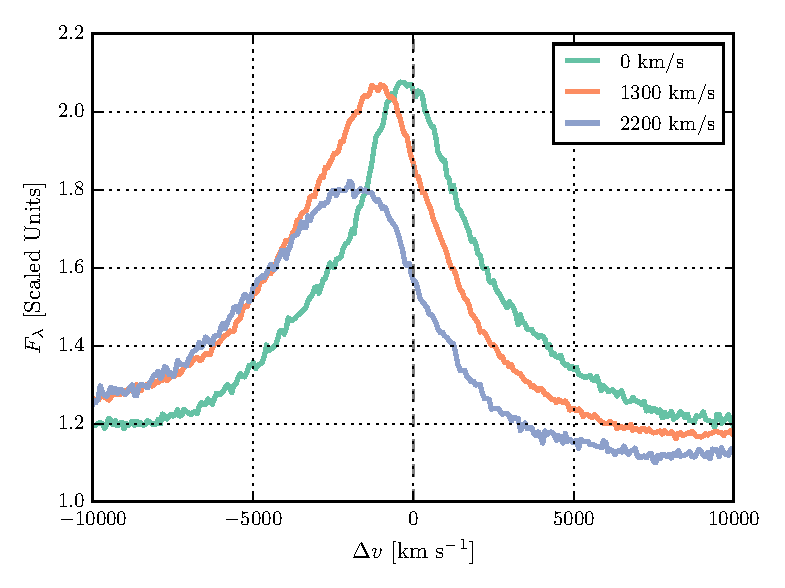
\includegraphics[width=0.9\linewidth]{figures/chapter03/civ_composites.pdf}
    \caption[{Composite spectra of the \ion{C}{IV} emission-line as a function of \ion{C}{IV} blueshift.}]{Composite spectra of the \ion{C}{IV} emission-line as a function of \ion{C}{IV} blueshift for SDSS DR$7$ quasars. Quasars classified as BALs, or possessing strong associated absorbers have been excluded, and the composite spectra shown are derived using an arithmetic mean of a minimum of $200$ spectra at each blueshift. Virtually the entire \ion{C}{IV}-profile appears to shift blueward and the change in line shape is not simply an enhancement of flux in the blue wing of a still identifiable symmetric component. In order of increasing \ion{C}{IV} blueshift, the composite spectra have FWHM $4870$, $5610$, and $6770$\,\kms\, and EQW $33.1$, $31.6$, and $28.8$\,\AA.}
    \label{fig:civ_composites}
\end{figure}

Figure~\ref{fig:civ_composites} shows the shape of the \ion{C}{IV}-emission in composite spectra constructed from SDSS DR$7$ quasars as a function of \ion{C}{IV} blueshift. 
The profiles show how, at large values of blueshift ($\gtrsim2000$\,\kms) the \ion{C}{IV}-profile is displaced to the blue by amounts comparable to the FWHM of the profile.
At fixed emission-line EQW, virtually the entire \ion{C}{IV}-profile appears to shift blueward and the change in line shape is not simply an enhancement of flux in the blue wing of a still identifiable symmetric component. 
While gravity almost certainly plays a key role, determining the escape velocity for out-flowing material for example, it is clear that the virial assumption, on which single-epoch BH mass measurements are predicated, is not straightforwardly applicable for the \ion{C}{IV} emission-line in quasars exhibiting large blueshifts.
In general, researchers studying quasar demographics at high-redshift adopt estimates of BH masses based on the width of \ion{C}{IV}-emission, without reference to the blueshift of the \ion{C}{IV}-emission \citep[e.g.][]{vestergaard04,kollmeier06,gavignaud08,vestergaard08,vestergaard09,kelly10,kelly13}.  
As a consequence, BH masses derived from \ion{C}{IV} emission-line velocity-widths are systematically biased compared to masses from the Balmer lines \citep[e.g.][]{shen08,shen12}. 

As highlighted by \citet{richards11}, the sample of reverberation mapped quasars includes a restricted range of the \ion{C}{IV} emission-line shapes seen in the quasar population. 
In particular, the reverberation mapped objects generally possess high \ion{C}{IV} EQWs and low \ion{C}{IV}-blueshifts. 
Nevertheless, the derived scaling relations based on the reverberation-mapped sample are regularly applied to the quasar population with low \ion{C}{IV} EQWs and/or large \ion{C}{IV}-blueshifts, where any non-virial outflow-related contribution to the dynamics is significant. 

In recent literature, attempts have been made to minimise the influence of the systematic non-virial contribution to the \ion{C}{IV} emission on estimates of the BH mass. 
Strategies include (i) significantly reducing the dependence of the derived masses on the emission-line velocity width (e.g. from the $\Delta V^2$ dependence predicted assuming a virialized BLR to just $\Delta V^{0.56}$ in \citealt{park13}; see also \citealt{shen12}), (ii) adopting a measure of emission-line velocity-width that is relatively insensitive to changes in the core of the emission-line profile \citep[e.g.][]{denney13} and (iii) estimating the amplitude of the non-virial contribution to the \ion{C}{IV} emission-line via comparison with other ultra-violet emission-lines (e.g. \ion{Si}{IV}+\ion{O}{IV}$\lambda$$1400$ in \citealt{runnoe13} and \citealt{brotherton15}).
The increased number of quasars with high-quality spectra that cover both the observed-frame optical (where the redshifted \ion{C}{IV} appears) and near-infrared (where \hb and \ha lie) enables us to take a rather different approach in this chapter.
We will use properties of the \ion{C}{IV} emission-line itself to reduce, or even remove, the systematic bias in the BH mass estimates. 
Specifically, using the low-ionisation Balmer lines \ha and \hb as reliable proxies for the virial velocity, we will measure empirically the systematic bias in \ion{C}{IV}-based virial BH mass estimates as a function of the \ion{C}{IV} emission-line blueshift.

\section{Quasar sample}

We have compiled a sample of $307$ non-BAL quasars at redshifts $1.5 < z < 4$ with both optical and near-infrared spectra.  
Reliable emission-line properties were measured for $230$ quasars (Section~\ref{sec:flagged_spectra}), with $164$ possessing \ha line measurements and $144$ \hb line measurements.  
This will allow us to directly compare virial BH mass estimates based on the \ion{C}{IV} line-width with estimates based on the line-widths of the low-ionisation Balmer lines \ha and \hbns.  
The sample is considerably larger than previous studies of the rest-frame optical spectra of high-$z$ quasars \citep[e.g.][]{shen12}. 
As we demonstrate in Section~\ref{sec:effectiveness}, the quasars have \ion{C}{IV} blueshifts of up to $\sim5000$\,\kms, and span virtually the full range of blueshifts observed in the population. 

The near-infrared data has been described in Chapter~\ref{ch:nirsample} and the telescopes/spectrographs used are summarised in Table~\ref{tab:specnums_ch3}. 
Corresponding optical spectroscopy was obtained from the SDSS ($70$ quasars), BOSS ($126$ quasars) and Hamburg-ESO surveys ($15$ quasars), and with VLT/UVES ($11$ quasars) and VLT/XSHOOTER ($8$ quasars). 
Many of the quasars in the SDSS DR$7$ catalogue have been re-observed as part of BOSS.
As the BOSS spectra typically have higher S/N than the SDSS DR$7$ spectra, we have used the BOSS spectra when available.
Once more, further details are provided in Chapter~\ref{ch:nirsample}. 
We have sub-divided our sample into two overlapping groups: quasars with reliable \ha line measurements (the `\ha sample') and quasars with reliable \hb measurements (the `\hb sample').

\begin{table}
  \footnotesize
  \centering
    \begin{tabular}{cccc} 
    \hline
    Spectrograph & Telescope & \ha Sample & \hb Sample \\
    \hline
    FIRE       & MAGELLAN & $18$ & $19$ \\
    GNIRS      & GEMINI-N & $22$ & $17$ \\
    ISAAC      & VLT      & $0$  & $4$ \\
    LIRIS      & WHT      & $15$ & $0$ \\
    NIRI       & GEMINI-N & $0$  & $12$ \\
    SINFONI    & VLT      & $2$  & $25$ \\
    SOFI       & NTT      & $47$ & $23$ \\
    TRIPLESPEC & ARC-$3.5$m & $33$ & $20$ \\
    TRIPLESPEC & P$200$     & $23$ & $19$ \\
    XSHOOTER   & VLT      & $4$  & $7$ \\
    \hline
    \multicolumn{2}{c}{Total} & $164$ & $144$ \\
    \hline
    \end{tabular}
      \caption{The numbers of quasars with reliable \ha and \hb line measurements, and the spectrographs and telescopes used to obtain the near-infrared spectra.}
  \label{tab:specnums_ch3}
\end{table}

\section{Spectral measurements}
\label{sec:spec_measures}

Conventionally, single-epoch virial estimates of the BH mass are a function of the line-of-sight velocity width of a broad emission-line and the quasar luminosity. 
The velocity width is a proxy for the virial velocity in the BLR and, as revealed in reverberation-mapping studies, the luminosity is a proxy for the typical size of the BLR \citep[the $R_{\text{BLR}}-L$ relation; e.g.][]{kaspi00,kaspi07}. 
Most reverberation mapping campaigns have employed \hb time-lags and velocity widths, but the line-widths of \ha and \ion{Mg}{II} have been shown to yield consistent BH masses \citep[e.g.][]{mclure02,greene05b,onken08,shen08,wang09,rafiee11,mejia-restrepo16}. 
In Section~\ref{sec:hahbcomparison}, we verify that the \ha and \hb line-widths yield consistent BH masses for the $99$ quasars in our sample with measurements of both.     

In our work, a robust measure of the \ion{C}{IV} emission-line `blueshift' provides the basis for the corrected \ion{C}{IV} velocity-width measurements, and hence BH masses.
The effectiveness of the scheme is validated via a direct comparison of the \ion{C}{IV} velocity-widths to the Balmer emission velocity-widths in the same quasars. 
Our process is as follows. 
First, an accurate measure of the quasar's systemic redshift is required, for which we adopt the centre of the Balmer emission, where the centre, $\lambda_{\text{half}}$, is the wavelength that bisects the cumulative total flux. 
Balmer emission centroids are available for all quasars in the catalogue but we verify that the measure is relatively unbiased through a comparison of the centroids to the wavelength of the peak of the narrow [\ion{O}{III}]\l$5008$ emission-line for the subset of spectra where both are available (Section~\ref{sec:zsys}). 
Second, the blueshift of the \ion{C}{IV} emission-line is determined. 
Again, we adopt the line centroid to provide a robust measure of the \ion{C}{IV} emission blueshift.
The blueshift (in \kms) is defined as

\begingroup\makeatletter\def\f@size{11}\check@mathfonts
\begin{eqnarray}
\label{eq:civblueshift}
c \times \frac{1549.48\,{\mathrm \AA}-\lambda_{\text{half}}}{1549.48\,{\mathrm \AA}}
\end{eqnarray}
\endgroup

\noindent where $c$ is the velocity of light and $1549.48$\,\AA\, is the rest-frame wavelength for the \ion{C}{IV} doublet\footnote{The adopted \ion{C}{IV} rest-frame wavelength assumes an optically thick BLR, in which case the contribution from each component is equal. Adopting a $2:1$ ratio (appropriate for an optically thin BLR) changes the blueshifts by $\sim80$\,\kms.}. 
Positive blueshift values indicate an excess of emitting material moving towards the observer and hence out-flowing from the quasar. 

Emission-line velocity widths are derived from the FWHM of the lines but we also compute the line dispersion (calculated from the flux-weighted second moment of the velocity distribution) as some authors have claimed this provides a better estimate of the virial velocity \citep{denney13}. 

To minimise the impact of the finite S/N of the quasar spectra and the presence of absorption features superposed on the broad emission-lines we first fit a parametric model to the continuum and the emission-lines. 
The particular form of the model parametrisations is not important and the fits are used only to provide robust line parameters, such as the centroid $\lambda_{\text{half}}$, and FWHM, which are measured non-parametrically from the best-fitting model. 
The models used and the fitting procedure are described below. 
The issues involved in deriving parameters for broad emission-lines from spectra of modest S/N -- for example, subtraction of narrow line emission, subtraction of \ion{Fe}{II} emission -- have been covered comprehensively by other authors \citep[e.g.][]{shen11,shen12,denney13,shen16a} and, as far as possible, we follow standard procedures described in the literature. 

\subsection{Modelling \ion{C}{IV}}
\label{sec:civ}

We first define a power-law continuum, $f(\lambda) \propto \lambda^{-\alpha}$, with the slope, $\alpha$, determined using the median\footnote{The median is used to improve the robustness of the continuum estimate from the relatively small wavelength intervals.} values of the flux in two continuum windows at $1445$-$1465$ and $1700$-$1705$\,\AA\, (the same wavelengths as adopted by \citealt{shen11}). 
The continuum emission is subtracted from the spectra, which is then transformed from wavelength units into units of velocity relative to the rest-frame line-transition wavelength for the \ion{C}{IV} doublet.
The parametric model is ordinarily fit within the wavelength interval $1500$-$1600$\,\AA\, (corresponding to approximately $\pm 10\,000$\,\kms\, from the rest-frame transition wavelength), a recipe that is commonly adopted \citep[e.g.][]{shen11,denney13}. 
The line-window was extended if more than $5$ per cent of the total flux in the profile was present blueward of the short wavelength limit. 
Narrow absorption features, which are frequently found superimposed on \ion{C}{IV} emission, were masked out during the fit. 

The \ion{C}{IV} emission was fit with sixth-order Gauss-Hermite (GH) polynomials, using the normalisation of \citet{marel93} and the functional forms of \citet{cappellari02}. 
We allowed up to six components, but in many cases a lower order was sufficient ($40$ and $45$ per cent were fit with second- and fourth-order GH polynomials respectively).
GH polynomials were chosen because they are flexible enough to model the often very asymmetric \ion{C}{IV} line profile. 
The flip-side of this flexibility, however, is that the model has a tendency to over-fit when spectra possess low S/N. 
The fits were therefore carefully checked visually and the number of components reduced if over-fitting was evident.

We find that using the commonly employed three-Gaussian component model, rather than the GH polynomials, resulted in only marginal differences in the line parameters. 
Our best-fit parameters are also in good agreement with \citet{shen11}, who employ a multi-Gaussian parametrisation. 
In Figure~\ref{fig:shen_comparison_civ} we compare our measurements of the \ion{C}{IV} FWHM from the $71$ SDSS DR$7$ spectra in our sample with the measurements published in \citet{shen11}. 
There is a very strong agreement between our measurements, with a scatter (median absolute deviation) of $190$\,\kms. 

\begin{figure}
    \centering 
    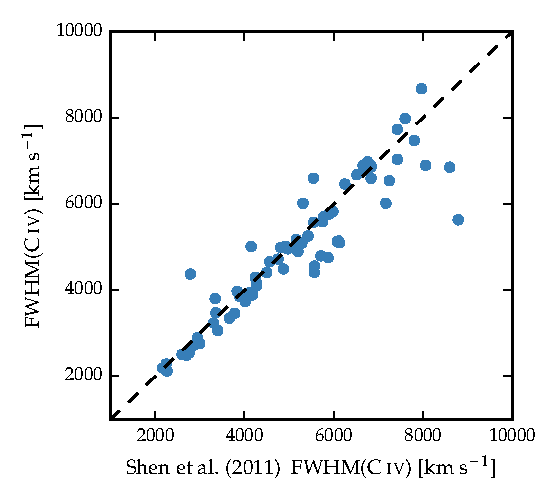
\includegraphics[width=0.8\linewidth]{figures/chapter03/shen_comparison_civ.pdf} 
    \caption[{Demonstration of the effectiveness of \ion{C}{IV} line parameter estimation scheme.}]{Demonstration of the effectiveness of our line parameter estimation scheme via a comparison of the \ion{C}{IV} FWHM with \citet{shen11}.} 
    \label{fig:shen_comparison_civ}
\end{figure}

\subsection{Modelling \ha}
\label{sec:ha}

A power-law continuum is fit using two continuum windows at $6000$-$6250$ and $6800$-$7000$\,\AA. 
The continuum-subtracted flux is then fit in the wavelength interval $6400-6800$\,\AA. 
We adopt a rest-frame transition wavelength of $6564.89$\,\AA\, to transform wavelengths into equivalent Doppler velocities. 
The broad component of \ha is fit using one or two Gaussians, constrained to have a minimum FWHM of $1200$\,\kms. When two Gaussians are used, the velocity centroids are constrained to be the same.

The emission-line profiles of both \hb and \ha frequently include a significant narrow component from the physically more extended NLR. 
Additional Gaussian components were included in our parametric model to fit the narrow component of \ha as well as [\ion{N}{II}]\ll$6548$,$6584$ and [\ion{S}{II}]\ll$6717$,$6731$.
This resulted in a better fit to the observed flux in $50$ per cent of cases. 
We impose a $1200$\,\kms\, upper limit on the FWHM of all narrow lines and the amplitudes of all components must be non-negative.
The relative flux ratio of the two [\ion{N}{II}] components is also fixed at the expected value of $2.96$.
In $70$ per cent of the spectra the [\ion{O}{III}]\ll$4960$,$5008$ doublet is detected at moderate S/N in the \hb region. 
In these cases the peak of the [\ion{O}{III}] is used to fix the velocity offsets and the FWHMs of the narrow line components in the \ha region.  
For spectra where the [\ion{O}{III}] doublet does not constrain the velocity and FWHM accurately, the narrow emission in the \ha and \hb regions are fitted independently but, for each region, the individual narrow-line velocity offsets and the FWHMs are constrained to be identical. 
In these objects the narrow line contribution is generally weak, and so does not have a large effect on the line parameters we measure for the broad component.   

The model described above is very similar to the one described in \citet{shen12} and \citet{shen11}, the only major differences being that we do not fit the \ha and \hb emission regions simultaneously and we fix the centroids of the Gaussian components used to fit the broad emission.
In Figure~\ref{fig:shen_comparison_ha} we plot our \ha FWHM measurements against the measurements published in \citet{shen12}, for $51$ quasars in common to both samples.
There is a strong correlation and a scatter of $300$\,\kms. 

\begin{figure}
    \centering 
    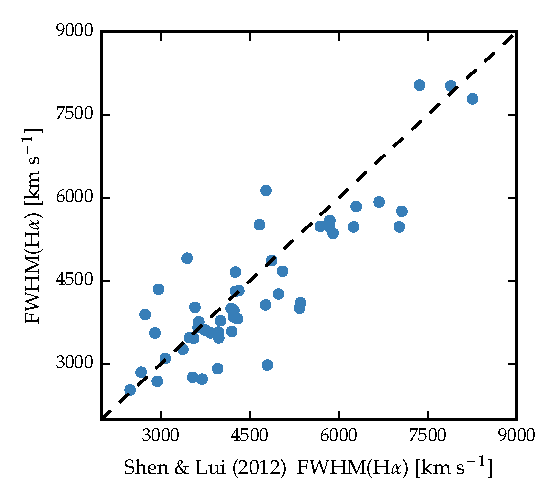
\includegraphics[width=0.8\linewidth]{figures/chapter03/shen_comparison_ha.pdf} 
    \caption[{Demonstration of the effectiveness of \ha line parameter estimation scheme.}]{Demonstration of the effectiveness of our line parameter estimation scheme via a comparison of the \ha FWHM with \citet{shen12}.} 
    \label{fig:shen_comparison_ha}
\end{figure}

\subsection{Modelling \hb and [\ion{O}{III}]}
\label{sec:hb}

Emission from optical \ion{Fe}{II} is generally strong in the vicinity of \hbns.
We therefore fit a combination of a power-law continuum and an optical \ion{Fe}{II} template -- taken from \citet{boroson92} -- to two windows at $4435$-$4700$ and $5100$-$5535$\,\AA. 
The \ion{Fe}{II} template is convolved with a Gaussian, and the width of this Gaussian, along with the normalisation and velocity offset of the \ion{Fe}{II} template, are free variables in the pseudo-continuum fit.
We use the same model to fit the broad and narrow components of \hb as was used with \hans. 
Each line in the [\ion{O}{III}] doublet is fit with two Gaussians, to model both the systemic and any outflow contributions. 
The peak flux ratio of the [\ion{O}{III}] $4960$\,\AA\, and $5008$\,\AA\, lines is fixed at $1$:$3$. 
As for the fit to the narrow lines in the spectral region around \hans, the width and velocity offsets of all the narrow components are set to be equal, and an upper limit of $1200$\,\kms\, is placed on the FWHM. 

The parametric model we fit to the \hbns/[\ion{O}{III}] emission region was very similar to the model employed by \citet{shen16a}. 
In Figure~\ref{fig:shen_comparison_hb} we plot our \hb FWHM measurements against the measurements published in \citet{shen16a}, for $39$ quasars in common to both samples. 
As expected, we observe a very tight correlation, with a scatter of $270$\,\kms. 

\begin{figure}
    \centering 
    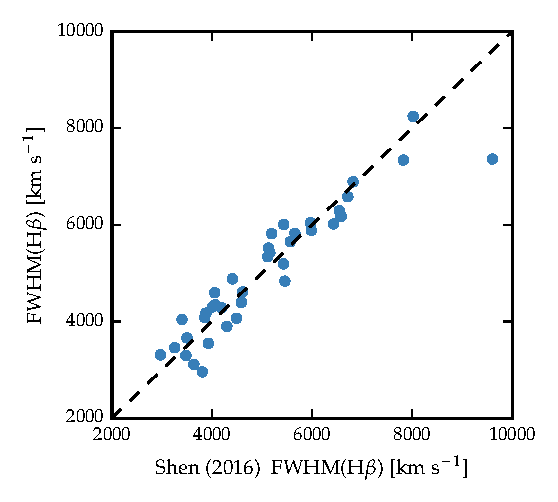
\includegraphics[width=0.8\linewidth]{figures/chapter03/shen_comparison_hb.pdf} 
    \caption[{Demonstration of the effectiveness of \hb line parameter estimation scheme.}]{Demonstration of the effectiveness of our line parameter estimation scheme via a comparison of the \hb FWHM with \citet{shen16a}.} 
    \label{fig:shen_comparison_hb}
\end{figure}

\subsection{Fitting procedure}

Model parameters were derived using a standard variance-weighted least-squares minimisation procedure employing the Nelder-Mead algorithm. 
Prior to the fit, the spectra were inspected visually and regions significantly affected by absorption or of low S/N were masked out.

In Figure~\ref{fig:examplegrid} we present our parametric fits to the \ion{C}{IV}, \ha and \hb emission-lines in a handful of quasars, which have been chosen to illustrate the range of spectrum S/N and line shapes in the sample.  
The Doppler velocities have been shifted so that the \ha emission-line centroid is at $0$\,\kms. 
The $y$-axes of the data-minus-model residual plots have been scaled by the spectrum flux errors.
The median reduced-$\chi^2$ values in our \hans, \hb and \ion{C}{IV} fits are $0.96$, $1.58$, and $0.91$ respectively and, in general, there are no strong features observable in the model residuals. 
The only significant features seen in the residual \ion{C}{IV} spectra correspond to the location of narrow absorption-lines which were excluded in the fitting procedure.

Table~\ref{tab:bhm-specmeasure} includes the line parameters of our best-fitting model for each line.

\begin{figure}
    \centering
    
\includegraphics[width=\linewidth]{figures/chapter03/example_spectrum_grid.pdf} 
    \caption[{Model fits to \hans, \hbns, and \ion{C}{IV} emission in four quasars.}]{Model fits to continuum-subtracted \hans, \hbns, and \ion{C}{IV} emission in four quasars. The data is shown in grey, the best-fitting parametric model in black, and the individual model components in orange. The centroid of the broad \ha emission is used to set the redshift, and $\Delta{v}$ is the velocity shift from the line rest-frame transition wavelength. The S/N is indicated and is measured in a region of the continuum and quoted per $150$\,\kms\, pixel. Below each line we plot the data minus model residuals, scaled by the errors on the fluxes.} 
    \label{fig:examplegrid}
\end{figure}


\subsection{Spectra removed from sample}
\label{sec:flagged_spectra}

\begin{table}
  \footnotesize
  \centering
    \begin{tabular}{cccc}
    \hline
    & & \ha sample & \hb sample \\ 
    \hline
    \multicolumn{2}{c}{Total} & $194$ & $279$ \\
    \hline
    \hans/\hbns & Wavelength & $6$ & $27$ \\
    & S/N & $8$ & $83$ \\
    \hline
    \ion{C}{IV} & Wavelength & $6$ & $5$ \\
    & S/N & $4$ & $12$ \\
    & Absorption & $6$ & $8$ \\
    \hline
    \multicolumn{2}{c}{Total remaining} & $164$ & $144$ \\
    \hline
    \end{tabular}
    \caption[{The number of spectra removed from our sample by different quality cuts.}]{The number of spectra removed from our sample by the cuts described in Section~\ref{sec:flagged_spectra}.}
  \label{tab:flagged_spectra}
\end{table}


Through visual inspection we flagged and discarded the spectra of quasars for which reliable emission-line parameters could not be obtained.

First, we flagged emission-lines in spectra that possessed insufficient S/N. 
A single minimum S/N threshold was not entirely effective and, instead, spectra were flagged when it was judged conservatively that no meaningful constraints could be placed on the velocity centroid and/or width of the emission-line. 

Second, we flagged emission-lines where significant regions of the continuum and/or emission-line fell outside of the wavelength coverage of the spectra. 
Reliable continuum definition and subtraction is not straightforward for emission-lines so affected. 

Third, we flagged \ion{C}{IV} emission-lines because of strong, narrow absorption close to the peak of the line where reliable interpolation across the absorption, using our parametric model, was not possible. 

The number of spectra that are removed by each cut is given in Table~\ref{tab:flagged_spectra} and the distribution in redshift and luminosity is shown in Figure~\ref{fig:flagged_spectra}. 
Unsurprisingly, there is a preferential removal of intrinsically faint quasars, whose spectra can be of poorer S/N, and a loss of quasars at redshifts $z\sim2.6$ where the \ha emission falls at the edge of the $K$-passband.
\hb is much weaker than \hans, and the \hb spectra are generally of lower S/N. 
As a result, the fraction of \hb spectra that are flagged -- $39$ per cent -- is particularly high.   

\begin{figure}[h!]
    \captionsetup[subfigure]{labelformat=empty}
    \centering
    \subfloat[\label{fig:flagged_spectra_a}]{}
    \subfloat[\label{fig:flagged_spectra_b}]{}
    \subfloat[\label{fig:flagged_spectra_c}]{}
    \subfloat[\label{fig:flagged_spectra_d}]{}
    \subfloat[]{{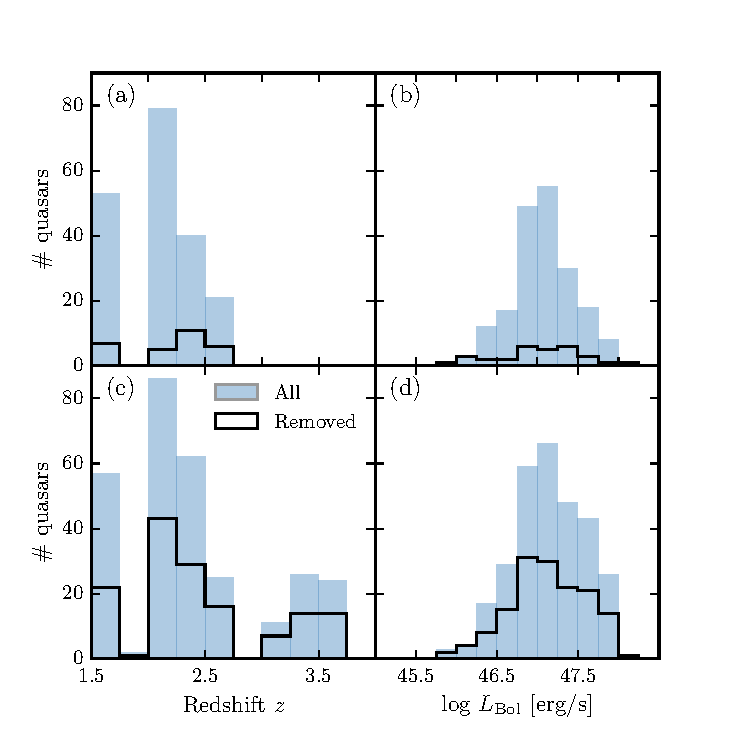
\includegraphics[width=\textwidth]{figures/chapter03/flagged_spectra.pdf} }}
    \caption[{The redshift and luminosity distributions of the spectra removed from sample.}]{The redshift and luminosity distributions of the spectra removed from our \hans/\ion{C}{IV} (a, b) and \hbns/\ion{C}{IV} (c, d) samples.} 
    \label{fig:flagged_spectra}
\end{figure}

\subsection{Emission-line parameter uncertainties}
\label{sec:ch3_param_errors}

To calculate realistic uncertainties on our fitted variables, accounting for potential sources of systematic error such as the continuum subtraction, we employed a Monte Carlo approach. 
One thousand artificial spectra were synthesised, with the flux at each wavelength drawn from a Normal distribution (mean equal to the measured flux and standard deviation equal to the known error).
Our emission-line fitting recipe was then implemented on each of these mock spectra. 
The uncertainty in each parameter is given by the spread in the best-fitting values from the one thousand realisations of the fitting routine. 
In some cases the standard deviation of the parameter distribution was biased by extreme values caused by bad fits\footnote{In the analysis of the real spectra such fits are identified via visual inspection.}. 
We therefore chose to measure the spread in the parameter distribution by fitting a composite model with two Gaussian components -- one to model uncertainty in the parameter and the other any possible outlier component. 
The uncertainty in each line parameter was then taken to be the width of the narrower Gaussian. 
The uncertainties on all derived quantities, such as the BH mass, are propagated through by assuming that the uncertainties are uncorrelated and independent. 

\subsection{Contemporaneity of spectra}

The epochs of the near-infrared and optical spectra can differ by many years.
For example, the NTT SOFI spectra were taken $\sim14$ years after the SDSS spectra, and the VLT SINFONI spectra $20$ years or more after the Hamburg-ESO observations\footnote{Time differences in the quasar rest-frame are reduced by a factor of ($1 + z$).}.
If the broad emission-line profiles varied significantly on these time-scales the relation between the \ion{C}{IV} and Balmer line-width measurements could be blurred. 

Cases do exist of dramatic changes in quasar spectra over short time-scales, but this phenomenon is rare \citep{macleod16}. 
In our spectroscopic catalogue there are $112$ SDSS DR$7$ quasars which are re-observed in BOSS and included in the DR$12$ quasar catalogue. 
The mean time elapsed between the two sets of observations is $\sim8$ years. 
The root-mean-square difference in the \ion{C}{IV} FWHM measured from the BOSS and SDSS spectra is a modest $\simeq500$\,\kms. 
Differences in the S/N of the spectra will make a substantial contribution and the scatter due to true variations in the \ion{C}{IV} velocity-width will be significantly smaller than $500$\,\kms. 
We conclude therefore that any intrinsic changes with time do not materially affect the emission-line measurements.

\subsection{Quasar monochromatic luminosity}

Computing virial BH masses also requires the quasar luminosity in an emission-line free region of the continuum adjacent to the broad line being used. 
The luminosity is used as a proxy for the size of the BLR. 
The monochromatic continuum flux is generally measured at $1350$\,\AA\ for \ion{C}{IV} and $5100$\,\AA\, for \ha and \hbns. 
The calculation of these luminosities is described in Chapter~\ref{ch:nirsample}. 

As described in Chapter~\ref{ch:nirsample}, we estimate the uncertainties on the monochromatic luminosities to be $\sim0.3$\,dex. 
Given that the luminosity enters into the calculation of BH mass only as the square-root, the uncertainty on the luminosities does not make a large contribution to the uncertainties in the BH mass estimates.  

\subsection{Characterising the emission-line widths}
\label{sub:charemprof}

There has been a considerable degree of attention paid to the effectiveness of different velocity-width measures of the \ion{C}{IV}-emission; specifically, the line FWHM and the dispersion, $\sigma$, derived from the second-moment velocity \citep[e.g.][]{assef11, denney13}.
The FWHM and line dispersion trace different parts of the broad line velocity field, with the FWHM relatively more sensitive to any low-velocity core present and the line dispersion relatively more sensitive to the high velocity wings. 
In practice, the line dispersion is almost certainly a more robust velocity indicator when the assumptions underlying the virial-origin of the emission-line velocity width are true and the spectral S/N and resolution are adequate.
This was demonstrated by \citet{denney13} for a sample of quasars possessing a significantly smaller range in \ion{C}{IV}-blueshift than investigated here.

\begin{figure}
    \captionsetup[subfigure]{labelformat=empty}
    \centering 
    \subfloat[\label{fig:line_comparison_civ_a}]{}
    \subfloat[\label{fig:line_comparison_civ_b}]{}
    \subfloat[\label{fig:line_comparison_civ_c}]{}
    \subfloat[]{{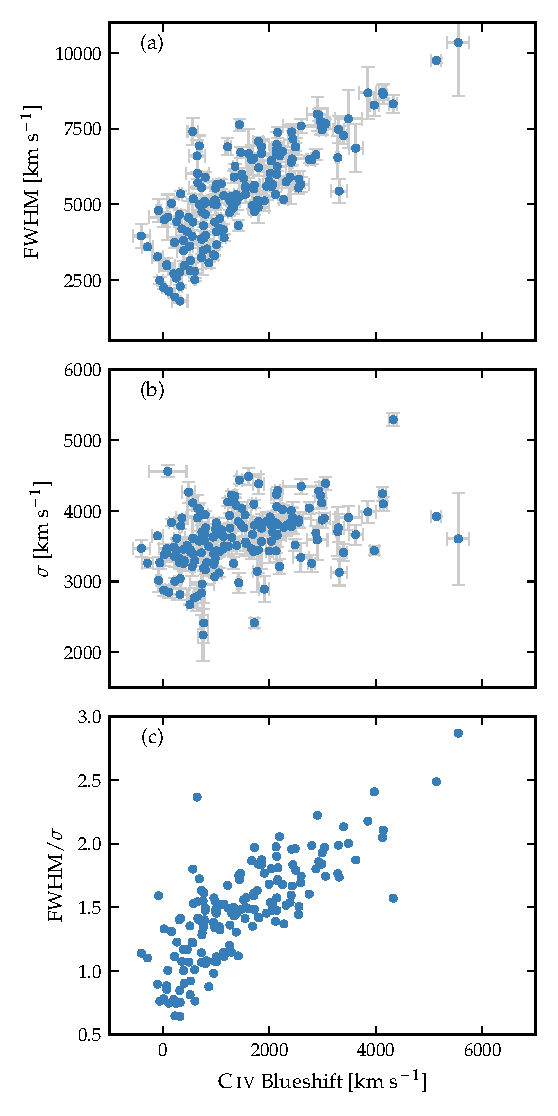
\includegraphics[width=0.8\textwidth]{figures/chapter03/civ_comparisons_paper2.pdf} }}
    \caption[{FWHM, dispersion and shape of \ion{C}{IV} as a function of the \ion{C}{IV} blueshift.}]{FWHM, dispersion ($\sigma$) and shape (FWHM/$\sigma$) of \ion{C}{IV} as a function of the \ion{C}{IV} blueshift.}
    \label{fig:line_comparison_civ}
\end{figure} 

In reality, however, as highlighted by \citet{denney12}, contributions to the \ion{C}{IV} emission-line profile from gas where virial motions do not dominate can be significant. 
Looking to the future, the results of the new reverberation-mapping projects \citep{shen15, kingoz15} will show what fraction of the \ion{C}{IV} emission-line, as a function of velocity, does reverberate for quasars with an extended range of \ion{C}{IV} emission shapes. 
The derivation of quantitative corrections to transform velocity-width measures from single-epoch to reverberation-only line profiles should then be possible. 

As such information is not yet available, there is a strong rationale for investigating whether the systematic changes in the \ion{C}{IV} emission-line profile can be used to improve the single-epoch BH mass estimates derived using the \ion{C}{IV} line. 
In Figure~\ref{fig:line_comparison_civ} we show how the \ion{C}{IV} FWHM, line dispersion, $\sigma$, and line shape, FWHM/$\sigma$, vary as a function of the blueshift. 
The \ion{C}{IV} FWHM is correlated with the blueshift, with the median FWHM of quasars with the largest blueshifts a factor of $2-3$ higher than quasars with only moderate blueshifts.
The dispersion, however, does not show a similarly strong systematic variation. 

Without knowledge of the \ion{C}{IV}-blueshifts, the dynamic range present in the FWHM and line dispersion measurements accords with the expectations from the study of \citet{denney13}; the factor of $\simeq4$ spread in the FWHM measurements indicating greater sensitivity to the emission-line profile shape than is the case for the dispersion, which varies by a factor of only $\lesssim2$.
Adopting a value of $1200$\,\kms\, to define `low' and `high' blueshift, the median \ion{C}{IV}-emission dispersion for the low and high-blueshift samples differ by only $10$ per cent. 
It follows, therefore, that while the dispersion provides a relatively line-profile independent measure of the velocity width for quasars where the underlying assumption regarding the virial-origin of the velocity width applies, quasars where the assumption is not true can be assigned apparently normal velocity-widths and hence potentially incorrect BH masses. 

To emphasise this point, in Figure~\ref{fig:civ_comparison} we overlay the \ion{C}{IV} line profiles of J$123611$+$112922$ and J$152529$+$292813$, whose dispersions are indistinguishable ($4168\pm271$ and $4303\pm128$\,\kms\, respectively). 
Notwithstanding the very similar dispersion values, the emission-line velocity fields differ dramatically and, therefore, the dispersion values cannot be measuring accurately the virial-induced velocity spread of the \ion{C}{IV} emission in both quasars.

The analysis here, building on earlier work \citep[including][]{sulentic07,shen12}, confirms a link between \ion{C}{IV} emission-line shape and blueshift, raising the prospect of developing a blueshift-dependent correction to single-epoch BH mass estimates based on the \ion{C}{IV} line. 
Expressed in another way, we are interested in testing if the significant systematic change in line shape as a function of \ion{C}{IV} blueshift can be used to provide improved single-epoch BH masses from the \ion{C}{IV} emission-line.  
The tightness of the correlation we observe between the \ion{C}{IV} FWHM and blueshift implies that such an approach may be more effective than using the \ion{C}{IV} emission-line velocity dispersion without reference to blueshifts.
A further practical advantage is that, given the typical S/N of current survey-quality spectra, virial BH mass estimates for high-redshift quasars are usually based on the FWHM rather than the dispersion \citep[e.g.][]{shen11}, which, being strongly affected by the continuum placement, is often found to be difficult to measure robustly \citep[e.g.][]{mejia-restrepo16}. 

\begin{figure}
    \centering
    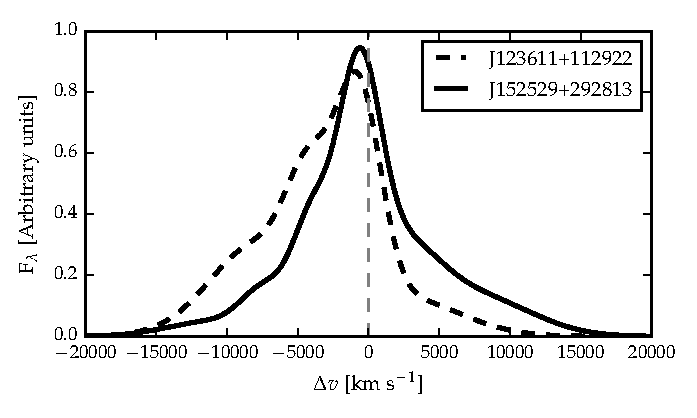
\includegraphics[width=\linewidth]{figures/chapter03/civ_comparison.pdf} 
    \caption[{Comparison of the \ion{C}{IV} line profiles of J$123611$+$112922$ and J$152529$+$292813$.}]{Comparison of the \ion{C}{IV} line profiles of J$123611$+$112922$ and J$152529$+$292813$. Notwithstanding the essentially identical dispersion values, the emission-line velocity fields differ dramatically and, therefore, the dispersion values cannot be measuring accurately the virial-induced velocity spread of the \ion{C}{IV} emission in both quasars. }
    \label{fig:civ_comparison}
\end{figure}

\section{An empirical correction to \ion{C}{IV}-based virial BH mass estimates}
\sectionmark{Correction to \ion{C}{IV}-based BH masses}

\subsection{\hans/\hb FWHM comparison}
\label{sec:hahbcomparison}

BH mass calibrations which use the width of the broad \hb emission-line as a proxy for the virial velocity are widely regarded as the most reliable, since most reverberation mapping employs the \hb line and the $R_{\text{BLR}}-L$ relation has been established using \hbns.
When \hb is not available, \ha has been shown to be a reliable substitute \citep[e.g.][]{greene05b,shen11,shen12}. 

We first compared the typical \ha and \hb profiles by constructing composite spectra. 
Individual spectra were first de-redshifted to the quasar rest-frame, and then interpolated on to a common wavelength grid with a $1$\,\AA\, resolution. 
The spectra were scaled by the mean flux in the interval $4700$-$5100$\,\AA\, (\hbns) and $6400$-$6800$\,\AA\, (\hans). 
The \ha and \hb lines in the median composite spectra are shown in Figure~\ref{fig:balmer_composite}.
\hb has a significantly broader profile than \ha in the composite spectra. 
This is to be expected if the density and/or ionisation parameter\footnote{Ionisation parameter: the ratio of the ionising photon number density to the particle density \citep[e.g.][]{peterson97}.} in the BLR decreases with increasing radii, because \hb is emitted preferentially over \ha when the density and/or ionisation parameter is higher \citep[e.g.][]{osterbrock89}. 

\begin{figure}
    \centering 
    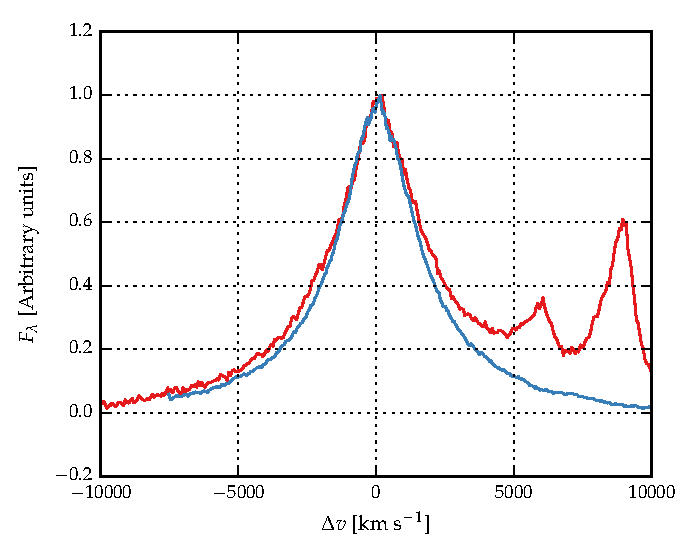
\includegraphics[width=0.8\linewidth]{figures/chapter03/ha_hb_composite.pdf} 
    \caption[{The \ha and \hb emission-line regions in the median composite spectrum.}]{The \ha and \hb emission-line regions in the median composite spectrum, shown as function of the velocity shift from the respective predicted line peak wavelengths. The background continuum and optical \ion{Fe}{II} emission (\hb only) has been modelled and subtracted. The line fluxes have been scaled in order for the profile shapes to be readily compared.}
    \label{fig:balmer_composite}
\end{figure}

In our sample, we have $99$ quasars with reliable measurements of both \ha and \hb lines. 
The line widths in individual objects are compared in Figure~\ref{fig:hahbcomp} and, as expected, a tight correlation is observed.  
\citet{greene05b}, using a sample of $162$ quasars with high S/N SDSS spectra at $z < 0.35$, established the following relation between the \ha and \hb FWHMs:

\begingroup\makeatletter\def\f@size{11}\check@mathfonts
\begin{eqnarray}
  \text{FWHM}(\text{H}\beta) = \left( 1.07 \pm 0.07 \right) \times 10^3 \left( \frac{ \text{FWHM}(\text{H}\alpha) }{10^3 ~\text{km}~\text{s}^{-1} } \right)^{(1.03 \pm 0.03)}.
\end{eqnarray}
\endgroup

\noindent The relation is shown as the dashed line in Figure~\ref{fig:hahbcomp}.
The root-mean-square scatter about this relation is $0.07$\,dex, compared to the $\sim0.1$\,dex reported by \citet{greene05b}. 
However, we find a systematic offset, in the sense that the \hb line-widths we measure are on average larger by $270$\,\kms\, than predicted by the \citet{greene05b} relation. 
As our sample covers higher redshifts and luminosities than the sample in \citet{greene05b}, we derive a new relation between the \ha and \hb FWHMs.       

\begin{figure}[t!]
    \centering 
    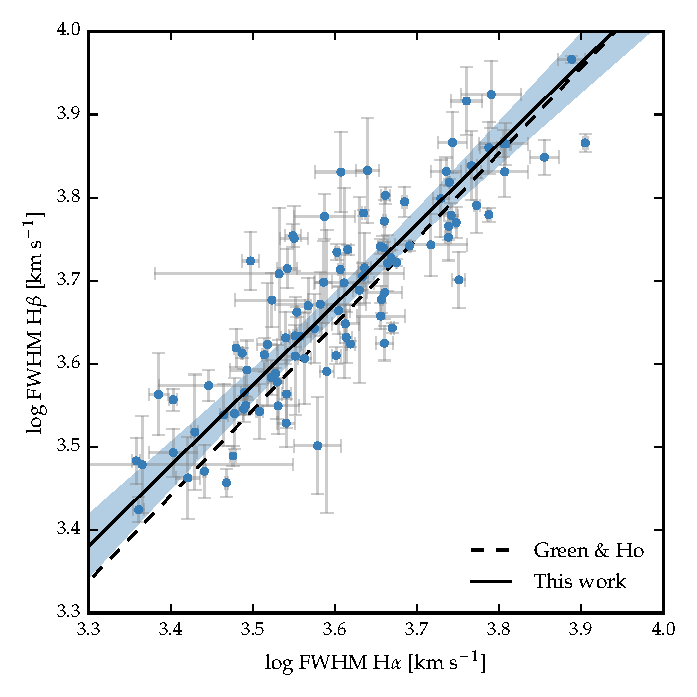
\includegraphics[width=0.8\columnwidth]{figures/chapter03/ha_hb_width_comparison.pdf} 
    \caption[{Comparison of \ha and \hb FWHM measurements for $99$ quasars.}]{Comparison of \ha and \hb FWHM measurements for $99$ quasars. The solid line is our best-fitting power-law model, and the blue-shaded region shows the $2$-$\sigma$ uncertainties on the model parameters. The dashed line is the relation found by \citet{greene05b} using a sample of $z<0.35$ SDSS AGN.} 
    \label{fig:hahbcomp}
\end{figure}

We assume a relation of the same form used by \citet{greene05b}, i.e. a simple power-law, and infer the model parameters by fitting a linear model (with slope $\alpha$ and intercept $\beta$) in log-log space.
The fit is performed within a Bayesian framework described by \citet{hogg10}. 
Each data point is treated as being drawn from a distribution function that is a convolution of the projection of the point's covariance tensor, $\Sigma_i^2$, with a Gaussian of variance $V$ representing the intrinsic variance in the data.
The log-likelihood is then given by 

\begingroup\makeatletter\def\f@size{11}\check@mathfonts
\begin{eqnarray}
  \text{ln} {\cal L} = - \sum_{i=1}^N \frac{1}{2} \text{ln}\left[2\pi\left(\Sigma_i^2 + V\right)\right] - \sum_{i=1}^N \frac{\Delta_i^2}{2[\Sigma_i^2 + V]} 
\end{eqnarray}
\endgroup

\noindent where $\Delta_i$ is the orthogonal displacement of each data point from the linear relationship. 
An advantage of this approach is that it allows a proper treatment of the measurement errors on both variables, which in this case are comparably large.
The model also makes the reasonable assumption that there is an intrinsic scatter in the relationship between the variables that is independent of the measurement errors.  
Following the suggestion by \citet{hogg10}, the linear model was parametrized in terms of ($\theta$,~$b_\bot$), where $\theta$ is the angle the line makes with the horizontal axis and $b_\bot$ is the perpendicular distance from the line to the origin.
Uniform priors were placed on these parameters, and the Jeffreys prior (the inverse variance) was placed on the intrinsic variance. 
The posterior distribution was sampled using a Markov Chain Monte Carlo (MCMC) method using the Python package \texttt{emcee} \citep{foreman13}. 

\begin{figure}[t!]
    \centering
    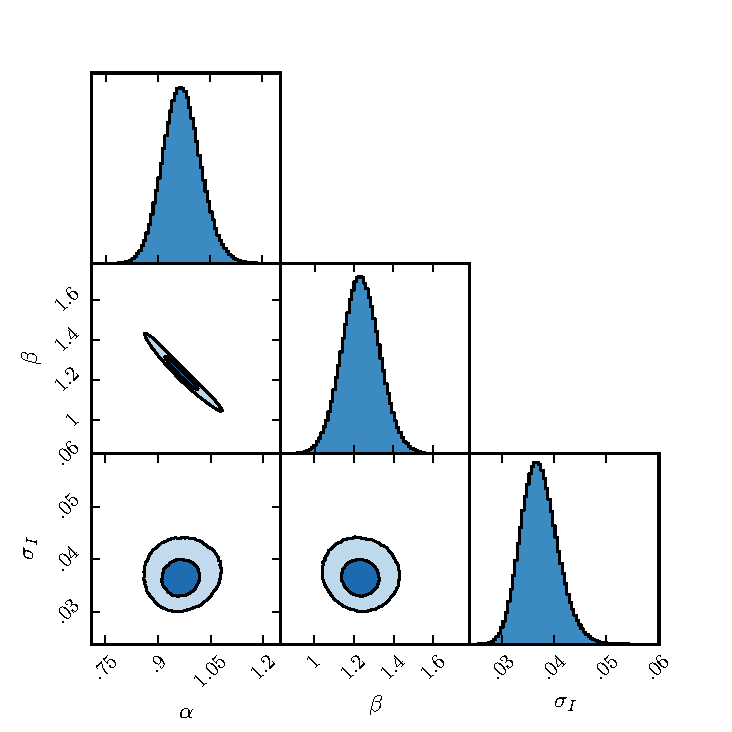
\includegraphics[width=0.8\columnwidth]{figures/chapter03/ha_hb_mcmc_parameters.pdf} 
    \caption[{Projections of the MCMC sampling of the posterior distribution from the fit to FWHM(\hans) and FWHM(\hbns).}]{One- and two-dimensional projections of the MCMC sampling of the posterior distribution from the fit to FWHM(\hans) and FWHM(\hbns) (Figure~\ref{fig:hahbcomp}). $\alpha$ is the power-law index, $10^\beta$ is the normalisation, and $\sigma_I$ is the intrinsic scatter. In the two-dimensional projections, $1$- and $2$-$\sigma$ contours are shown.} 
    \label{fig:ha_hb_mcmc_samples}
\end{figure}

The one- and two-dimensional posterior distributions are shown in Figure~\ref{fig:ha_hb_mcmc_samples}. 
The solid line in Figure~\ref{fig:hahbcomp} is the maximum likelihood solution

\begingroup\makeatletter\def\f@size{11}\check@mathfonts
\begin{eqnarray}
  \label{eq:ha2hb}
  \text{FWHM}(\text{H}\beta) = \left( 1.23 \pm 0.10 \right) \times 10^3 \left( \frac{\text{FWHM}(\text{H}\alpha)}{10^3 \text{km}\,\text{s}^{-1}} \right)^{0.97 \pm 0.05}
\end{eqnarray}
\endgroup

\noindent and the shaded region shows the $2$-$\sigma$ uncertainties on the model parameters.

As discussed above, our relation is displaced to slightly higher \hb FWHM than the \citet{greene05b} relation -- the offset is $210$\,\kms\, for a quasar with \ha FWHM $4500$\,\kms.  
We infer a power-law index that, although slightly shallower, is consistent with the \citet{greene05b} index within the quoted uncertainties. 
The intrinsic scatter in the data, $\sigma_I$, we infer from  the fit is $0.04$\,dex. 
This is smaller than the total scatter seen in Figure~\ref{fig:hahbcomp} ($0.06$\,dex), which suggests that measurement errors make a significant contribution to the total scatter in the relation. 

For $19$ of the $99$ quasars with \hb and \ha emission profiles, one of the two Gaussians used to reproduce the \hb profiles has a FWHM greater than $20$\,$000$\,\kms\, and a fractional contribution to the total \hb broad line flux greater than $30$ per cent \citep{marziani09,marziani13}.  
The very broad \hbns-component, which is not seen in the \ha profiles, may be an artefact of the fitting scheme.
A particular issue for \hb is the presence of \ion{Fe}{II} emission, often at a significant level.
Furthermore, additional lines could be contributing to the underlying continuum \citep[e.g. the \ion{He}{I}\ll$4922$,$5017$ doublet;][]{veron02,zamfir10}. 
If the \hb FWHM is calculated only from the narrower of the two Gaussian components, then the \hb FWHM decreases by $630$\,\kms\, on average, and the new relationship between the \ha and \hb FWHM is much closer to one-to-one. 
The \ion{C}{IV} FWHM relative to the \hans/\hb FHWM will be enhanced by $\sim15$ per cent, and so the \ion{C}{IV}-based BH masses relative to the Balmer-based masses will increase by $\sim30$ per cent. 

\subsection{Measuring the quasar systemic redshift}
\label{sec:zsys}

An accurate measure of the quasar's systemic redshift is required in order for the blueshift of the \ion{C}{IV} emission-line to be determined.
Balmer emission centroids are available for all quasars in the catalogue and so we use this to define the systemic redshift.

For $62$ and $86$ quasars in the \ha and \hb samples respectively narrow [\ion{O}{III}] emission is also detected with sufficient S/N to measure the line centroid. 
In the model fit to the \hb region the velocity centroids of the broad \hbns-line and the core component of the [\ion{O}{III}] emission were deliberately determined separately.
We find the intrinsic difference in the velocity centroids of the \ha and \hb emission and the narrow [\ion{O}{III}] emission to have a dispersion of $300$ and $400$\,\kms, which is very similar to the value found by \citet{shen16b}. 
However, the velocity centroid of the narrow component of the [\ion{O}{III}] emission is blueshifted by on average $250$\,\kms\, relative to the centroid of the broad Balmer line. 
Applying our parametric model fitting routine to the composite spectrum from \citet{hewett10}, which is constructed using relatively low redshift SDSS quasars with $L_{\text{Bol}}\sim10^{44}$\,erg\,s$^{-1}$, the centroids of the broad component of \hb and the narrow component of [\ion{O}{III}] are found to be at essentially identical velocities, suggesting that the blueshifting of narrow [\ion{O}{III}] could be luminosity dependent.

As described in Section~\ref{sec:spec_measures}, the broad components of \ha and \hb were modelled with up to two Gaussians, with identical velocity centroids. 
We also tested models with no constraints on the centroids of the two broad Gaussians, and measured the systemic redshift from the peak of the composite profile. 
With this set of models, the median difference between the [\ion{O}{III}]- and \hans(\hbns) based redshift estimates is reduced to $-100$($-120$)\,\kms, with a $290$($320$)\,\kms\, scatter. 
This suggests that there is a $\sim100$\,\kms\, systematic error in our Balmer-based redshift estimates. 
Regardless, since both the systematic offset and the scatter are small in comparison to the dynamic range in \ion{C}{IV} blueshifts ($\sim5000$\,\kms), the blueshift-based empirical correction we will derive does not depend on whether the broad Balmer emission or the [\ion{O}{III}] centroid is used to define the systemic redshift, or how the broad Balmer emission is parametrised. 

\subsection{Balmer/\ion{C}{IV} line widths as a function of \ion{C}{IV}-blueshift}
\label{sec:correction}

\begin{figure}
    \captionsetup[subfigure]{labelformat=empty} 
    \centering
    \subfloat[\label{fig:correction_ha_a}]{}
    \subfloat[\label{fig:correction_ha_b}]{}
    \subfloat[]{{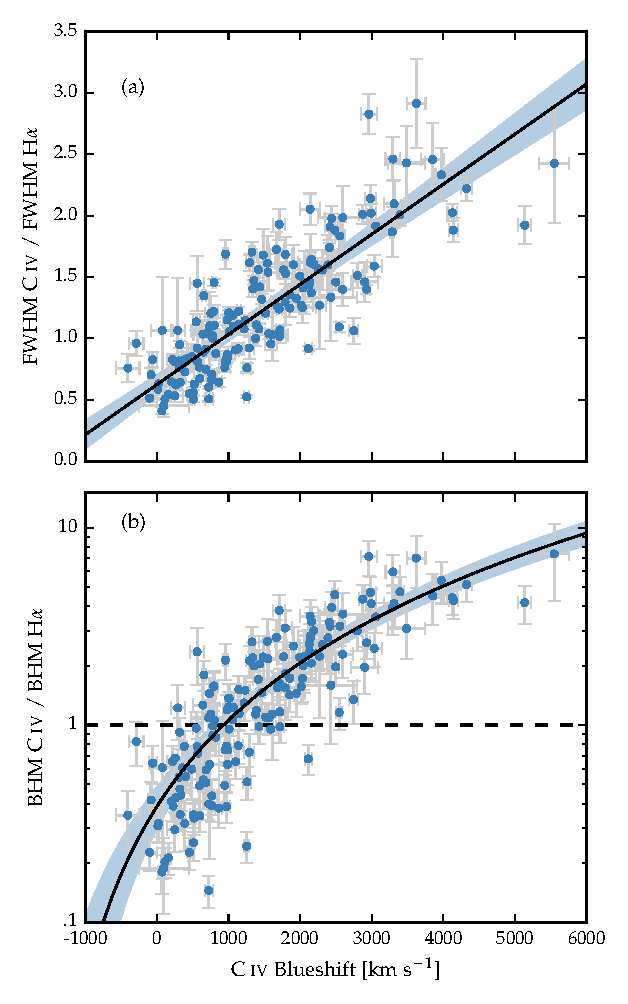
\includegraphics[width=0.9\textwidth]{figures/chapter03/fwhm_and_bhm_ha.pdf} }}
    \caption[{\ion{C}{IV} FWHM relative to \ha FWHM and \ion{C}{IV} based BH mass compared to \ha based mass, both as a function of the \ion{C}{IV} blueshift.}]{\ion{C}{IV} FWHM relative to \ha FWHM (a), and \ion{C}{IV} based BH mass (BHM) compared to \ha based mass (b), both as a function of the \ion{C}{IV} blueshift. The black line is our best-fit linear model, and the shaded region shows the $2$-$\sigma$ uncertainties on the slope and intercept. The \ha FWHM have been scaled to match the \hb FWHM using Equation~\ref{eq:ha2hb}.}  
    \label{fig:correction_ha}
\end{figure}

\begin{figure}
    \captionsetup[subfigure]{labelformat=empty} 
    \centering
    \subfloat[\label{fig:correction_hb_a}]{}
    \subfloat[\label{fig:correction_hb_b}]{}
    \subfloat[]{{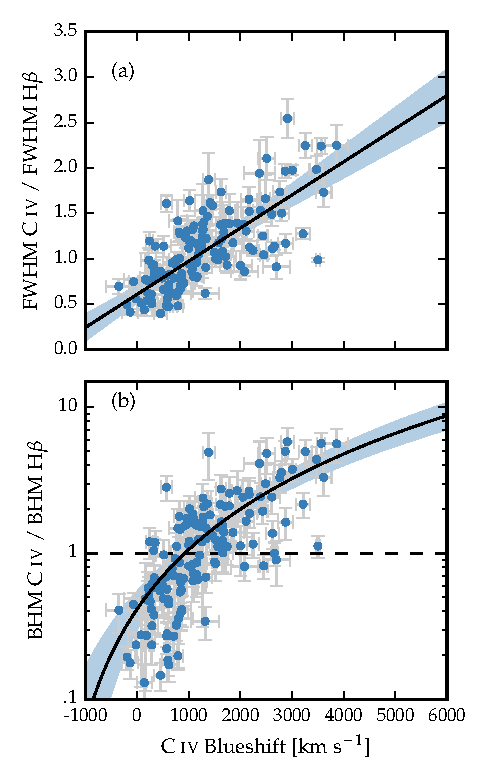
\includegraphics[width=0.9\textwidth]{figures/chapter03/fwhm_and_bhm_hb.pdf} }}
    \caption[{\ion{C}{IV} FWHM relative to \hb FWHM and \ion{C}{IV} based BH mass compared to \hb based mass, both as a function of the \ion{C}{IV} blueshift.}]{\ion{C}{IV} FWHM relative to \hb FWHM (a), and \ion{C}{IV} based BH mass (BHM) compared to \hb based mass (b), both as a function of the \ion{C}{IV} blueshift.}  
    \label{fig:correction_hb}
\end{figure}

In this section, we directly compare the \ion{C}{IV} and \hans/\hb line widths as a function of the \ion{C}{IV} blueshift. 
Because virial BH mass estimates are generally based on the \hb FWHM, we first convert our \ha FWHM measurements into equivalent \hb FWHM using Equation~\ref{eq:ha2hb}.  
In Figures~\ref{fig:correction_ha_a} and \ref{fig:correction_hb_a} we show the \ion{C}{IV} FWHM relative to both the (\hbns-scaled) \ha FWHM and the \hb FWHM, as a function of the \ion{C}{IV} blueshift. 

Employing the same Bayesian fitting framework described in Section~\ref{sec:hahbcomparison}, we fit independent linear models to the \ion{C}{IV} FWHM relative to the \ha and \hb FWHM as a function of the \ion{C}{IV} blueshift. 
As before, our model has an additional parameter representing any intrinsic scatter in the relationship between the variables which is independent of measurement errors.  
We also tested a model where some fraction of the data points (which is free to vary) is drawn from an outlier distribution, represented by a broad Gaussian centred on the mean of the data. 
We found, however, that the inferred outlier fraction was very low ($0.004$, corresponding to $\sim0.7$ data points) and so did not include such a component in our model. 

\begin{figure}
    \centering
    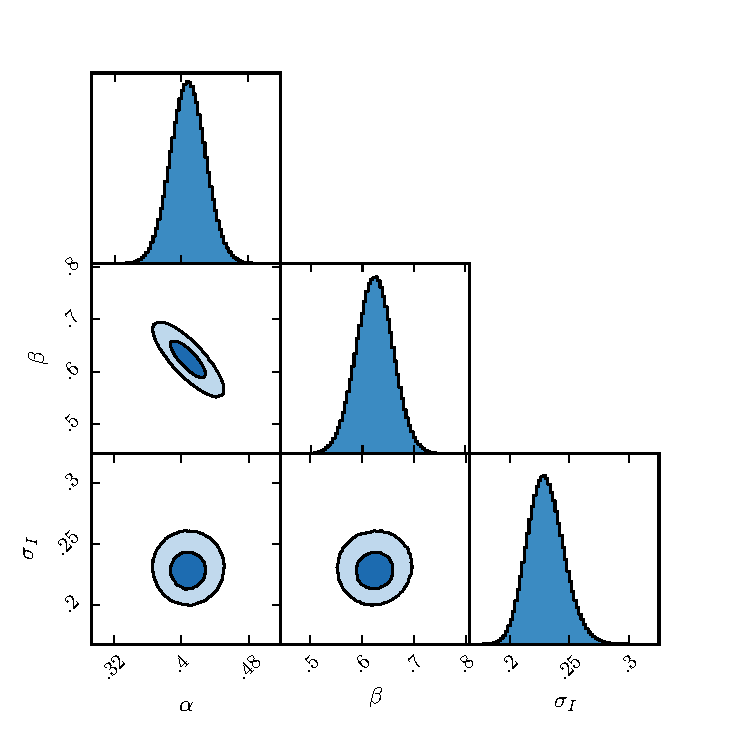
\includegraphics[width=0.8\textwidth]{figures/chapter03/civ_ha_mcmc_parameters.pdf} 
    \caption[{Projections of the MCMC sample of the posterior distribution for a linear fit to FWHM(\ion{C}{IV})/FWHM(\hans) as a function of the \ion{C}{IV} blueshift.}]{One- and two-dimensional projections of the MCMC sample of the posterior distribution for a linear fit to FWHM(\ion{C}{IV})/FWHM(\hans) as a function of the \ion{C}{IV} blueshift. In the two-dimensional projections we show $1$- and $2$-$\sigma$ contours. The posterior distribution for the linear fit to FWHM(\ion{C}{IV})/FWHM(\hbns), which we do not show, has a very similar appearance.} 
    \label{fig:mcmc_parameters}
\end{figure}

In Figure~\ref{fig:mcmc_parameters} we show the one- and two-dimensional projections of the posterior distribution from the linear fit to FWHM(\ion{C}{IV})/FWHM(\hans) as a function of the \ion{C}{IV} blueshift. 
The projections from the FWHM(\ion{C}{IV})/FWHM(\hbns) fit, which we do not show, have very similar appearances.
In Figure~\ref{fig:correction_ha_a} we plot the maximum likelihood model and the $2$-$\sigma$ uncertainties on the model parameters. 
The maximum likelihood line is given by  

\begingroup\makeatletter\def\f@size{10}\check@mathfonts
\begin{eqnarray}
    \label{eq:hafwhm}
    \text{FWHM}(\text{C}\,\textsc{iv}, \text{Corr.}) = \frac{\text{FWHM}(\text{C}\,\textsc{iv}, \text{Meas.})}{ (0.41\pm0.02) \left(\frac{\text{C}\,\textsc{iv}\, \text{Blueshift}}{10^3 \,\text{km}\,\text{s}^{-1}} \right) + (0.62\pm0.04)}
\end{eqnarray}
\endgroup

\noindent for the \ion{C}{IV}/\ha fit and 

\begingroup\makeatletter\def\f@size{10}\check@mathfonts
\begin{eqnarray}
    \label{eq:hbfwhm}
    \text{FWHM}(\text{C}\,\textsc{iv}, \text{Corr.}) = \frac{\text{FWHM}(\text{C}\,\textsc{iv}, \text{Meas.})}{ (0.36\pm0.03) \left(\frac{\text{C}\,\textsc{iv}\, \text{Blueshift}}{10^3 \,\text{km}\,\text{s}^{-1}} \right) + (0.61\pm0.04)}
\end{eqnarray}
\endgroup

\noindent for the \ion{C}{IV}/\hb fit. 
The intercepts of the two relations are consistent, while the difference between the slopes is only marginally inconsistent given the quoted uncertainties. 

The intrinsic scatter in the data about the linear relation we infer is $0.23 \pm 0.02$ and $0.25 \pm 0.02$ for the \ha and \hb fits respectively. 
The intrinsic scatter for the \ha fit is represented by the Normal probability density distribution shown in Figure~\ref{fig:intrinsic_scatter}. 
In the same Figure, we show the distribution of the orthogonal displacement of each data point from the best-fitting linear relationship. 
The two distributions are well-matched, which demonstrates that our model is a good representation of the data and the measurement errors on the data points are small relative to the intrinsic scatter.    

\begin{figure}[t!]
    \centering 
    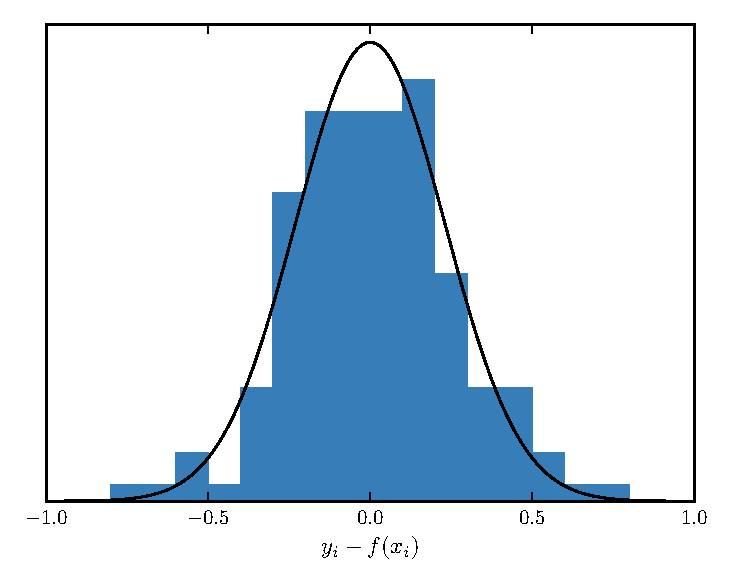
\includegraphics[width=0.7\textwidth]{figures/chapter03/intrinsic_scatter.pdf} 
    \caption[{The distribution of the orthogonal displacement of each data point from the best-fitting linear relationship in the fit to FWHM(\ion{C}{IV})/FWHM(\hans) as a function of the \ion{C}{IV} blueshift.}]{The distribution of the orthogonal displacement of each data point from the best-fitting linear relationship in the fit to FWHM(\ion{C}{IV})/FWHM(\hans) as a function of the \ion{C}{IV} blueshift (blue histogram). The black curve is a Normal distribution with a width equal to the intrinsic scatter in the population inferred from the fit. The two distributions are well-matched, which demonstrates that our model is a good representation of the data and the measurement errors on the data points are small relative to the intrinsic scatter.} 
    \label{fig:intrinsic_scatter}
\end{figure}

The overall (intrinsic and measurement) scatter about the best-fitting model is slightly higher when the \ion{C}{IV} line-widths are compared to \hb ($0.12$\,dex) than when compared to \ha ($0.10$\,dex). 
This is likely due, at least in part, to the generally higher S/N of the \ha emission. 
In addition, contributions from the strong [\ion{O}{III}] doublet and from \ion{Fe}{II} in the vicinity of \hb make de-blending the \hb emission more uncertain. 
As a consequence, for quasars where \ha and \hb are both measured, the mean uncertainty on the \ha FWHM is $130$\,\kms, compared to $340$\,\kms\, for \hbns. 

In the next section, we use both the \ha and \hb lines to calculate unbiased BH masses. 
However, we use the \ha measurements to derive an empirical \ion{C}{IV} blueshift based correction to the \ion{C}{IV} masses (Equation~\ref{eq:masscorrection}) because of the issues related to the accurate modelling of the \hbns-profile just described.  
An extra advantage, which is evident in Figures~\ref{fig:correction_ha_a} and \ref{fig:correction_hb_a}, is that the \ha sample has a better \ion{C}{IV} blueshift coverage. 
However, as can be seen from the similarity of Equations \ref{eq:hafwhm} and \ref{eq:hbfwhm}, our results would not change significantly were we instead to use the \hb sample. 

\subsection{\ion{C}{IV}-based virial BH mass estimates}

Virial BH masses were calculated using the widely adopted \citet{vestergaard06} calibrations. 
BH masses are computed using the line and continuum properties given in Table~\ref{tab:bhm-specmeasure}, and we convert our \ha emission-line velocity-width measures to predicted \hb widths using Equation~\ref{eq:ha2hb}.

In Figures~\ref{fig:correction_ha_b} and \ref{fig:correction_hb_b} the \ion{C}{IV}-based estimates are compared to the \hans/\hb estimates as a function of the \ion{C}{IV} blueshift. 
There is a strong systematic error in the \ion{C}{IV}-based masses as a function of blueshift, which is a direct consequence of the FWHM trend described in the previous section. 
The \ion{C}{IV} emission-based BH masses are in error by a factor of more than five at $3000$\,\kms\, in \ion{C}{IV} emission blueshift and the overestimate of the BH masses reaches a factor of $10$ for quasars exhibiting the most extreme blueshifts, $\gtrsim5000$\,\kms. 

The virial product is the product of the virial velocity squared and the BLR radius \citep[e.g.][]{shen13}, and is proportional to the BH mass. 
We use the corrected \ion{C}{IV} FWHM given by Equation~\ref{eq:hafwhm} as an indicator of the virial velocity, and adopt the same $R_{\text{BLR}}-L$ relation for the $1350$\,\AA\, continuum luminosity as \citet{vestergaard06} (i.e. $R_{\text{BLR}} \propto L^{0.53}$). 
To find the constant scaling factor necessary to transform the virial product into a BH mass we compute the inverse-variance weighted mean difference between the virial products and the \hans-based masses. 
The virial BH mass can then be expressed in terms of the corrected \ion{C}{IV} FWHM and monochromatic continuum luminosity at $1350$\,\AA:

\begingroup\makeatletter\def\f@size{10}\check@mathfonts
\begin{eqnarray}
  \label{eq:masscorrection}
  \text{MBH}(\text{C}\,\textsc{iv}, \text{Corr.}) = 10^{6.71}\left( \frac{ \text{FWHM}(\text{C}\,\textsc{iv}, \text{Corr.})}{10^3 \,\text{km}\,\text{s}^{-1}} \right)^2 \left( \frac{\lambda L_{\lambda} (1350 \text{\AA}) }{10^{44} \,\text{erg}\,\text{s}^{-1}}  \right)^{0.53}.
\end{eqnarray}
\endgroup

\noindent Given measured \ion{C}{IV} emission-line FWHM and blueshift, Equations~\ref{eq:hafwhm} and \ref{eq:masscorrection} can then be used to provide an unbiased estimate of the quasar BH mass.

\subsection{\ion{C}{IV}-derived BH masses at low \ion{C}{IV} blueshift}

Reverberation mapping measurements of nearby AGN have revealed the BLR to be stratified, with high-ionisation lines, including \ion{C}{IV}, emitted closer to the BH than low-ionisation lines, including \ha and \hb \citep[e.g.][]{onken02}.
\citet{vestergaard06} found that the \ion{C}{IV}-emitting region is at approximately half the radius of the \hbns/\ha emitting region.
Given the $\Delta V \propto R_{\text{BLR}}^{-0.5}$ virial relation, this leads to the prediction that the \ion{C}{IV} line widths should be $\simeq 1.4$ times broader than \hans/\hb for a given BH mass, and this expectation is reflected in the relative normalisations of the \citet{vestergaard06} \ion{C}{IV}- and \hbns-based BH mass calibrations.

In our sample, the median \ion{C}{IV}/\ha FWHM ratio is $0.97 \pm 0.31$ for the $77$ quasars with \ion{C}{IV} blueshifts $<1200$\,\kms.
This is significantly smaller than the predicted value of $1.4$. 
As a direct consequence of the empirically small \ion{C}{IV}/\ha FWHM ratio, the \ion{C}{IV}-derived BH mass estimates are systematically lower than the corresponding \hans-derived masses when the blueshift is small.
This can be seen in Figure~\ref{fig:correction_ha_b}, where for almost every quasar with a \ion{C}{IV} blueshift $<$$1200$\,\kms, the \ion{C}{IV}-derived BH mass is smaller than the corresponding \hans-derived mass.

\citet{denney12} used multiple-epoch spectra from reverberation mapping campaigns to isolate the part of the \ion{C}{IV} profile which is varying.
In some profiles they identified a non-varying core component, possibly originating from gas at larger radii than the BLR. 
In single-epoch spectra, both parts of the line -- varying and non-varying -- contribute to the measured FWHM. 
The gas at larger radii will enhance the profile at lower-velocity and lead to smaller FWHM values.
This could explain the low \ion{C}{IV}/\ha FWHM ratio observed in quasars with small \ion{C}{IV} blueshifts. 

\section{Practical application of the \ion{C}{IV}-based BH mass correction}
\sectionmark{Practical application}

\label{sec:ch3-application}

\subsection{Recipe for unbiased \ion{C}{IV} based BH masses}
\label{sec:ch3-recipe}

\subsubsection{Measuring the systemic redshift}

Equations~\ref{eq:hafwhm} and \ref{eq:masscorrection} together provide an un-biased estimate of the virial BH mass given the FWHM and blueshift of \ion{C}{IV}, together with the continuum luminosity at $1350$\,\AA. 
The FWHM is readily obtained, either directly from the data, or, via the fitting of a parametric model to the \ion{C}{IV} emission-line. 
The blueshift -- defined as the bisector of the cumulative line flux -- is also straightforward to measure and our preferred procedure is described in Section~\ref{sec:ch3-civmeasure}.
The only potential complication arises in establishing the quasar systemic redshift and hence defining the zero-point for the \ion{C}{IV}-blueshift measurement, since both the blueshift and the systemic redshift cannot be determined from \ion{C}{IV} alone. 
In practice, when rest-frame optical lines are accessible, as is the case for the quasar sample here, an accurate systemic redshift can be obtained. 
The [\ion{O}{III}] doublet and the Balmer lines all have velocity centroids very close to systemic, and the same is true for the broad \ion{Mg}{II} doublet. 
For quasars at very high redshifts, $z\sim6$, systemic redshifts can also be derived using the [\ion{C}{II}] $158$\,$\mu$m emission in the sub-millimetre band \citep[e.g.][]{venemans16}. 
However, in general, for example in determining the BH masses of quasars at redshifts $z>2$, if only the rest-frame ultra-violet region is available determining a reliable systemic redshift is non-trivial. 

The SDSS DR$7$ pipeline redshifts are not sufficiently reliable to measure the \ion{C}{IV} blueshift accurately because, in part, the \ion{C}{IV} emission-line itself contributes to the determination of the quasar redshifts. 
This is demonstrated in Figure~\ref{fig:civ_space_z_compare_a}, in which we plot the \ion{C}{IV}-blueshift versus \ion{C}{IV}-emission EQW using the SDSS pipeline redshifts and the blueshifts calculated by \citet{shen11}.  
A strong trend in the blueshift values as a function of line EQW is not evident in Figure~\ref{fig:civ_space_z_compare_a}; structure in the parameter space is being masked because the \ion{C}{IV} emission-line is itself being used in the determination of the quasar redshifts. 

\begin{figure}
    \captionsetup[subfigure]{labelformat=empty}  
    \centering 
    \subfloat[\label{fig:civ_space_z_compare_a}]{}
    \subfloat[\label{fig:civ_space_z_compare_b}]{}
    \subfloat[\label{fig:civ_space_z_compare_c}]{}
    \subfloat[]{{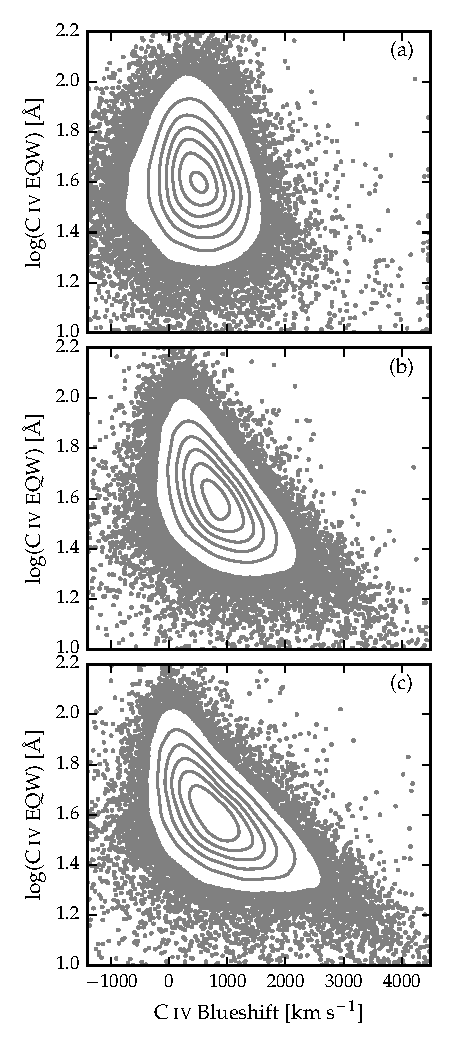
\includegraphics[width=8cm]{figures/chapter03/civ_space_z_compare.pdf} }}
    \caption[{Rest-frame EQW versus blueshift of the broad \ion{C}{IV} emission-line for SDSS quasars using three different redshift estimation schemes.}]{Rest-frame EQW versus blueshift of the broad \ion{C}{IV} emission-line for $32,157$ SDSS DR$7$ quasars at $1.6 < z < 3.0$. Panel (a) uses \ion{C}{IV} line parameters from \citet{shen11} and SDSS pipeline systemic redshifts. Panels (b) and (c) use systemic redshifts from \citet{hewett10} and Allen \& Hewett (2017, in preparation) respectively, and \ion{C}{IV} line measurements described in Section~\ref{sec:ch3-civmeasure}.} 
    \label{fig:civ_space_z_compare}
\end{figure}

The redshift-determination scheme of \citet{hewett10} provided much improved redshifts, not least because the redshift estimates for the majority of quasars were derived using emission-lines other than the \ion{C}{IV}-line itself. 
Figure \ref{fig:civ_space_z_compare_b} shows SDSS DR$7$ quasars in the same \ion{C}{IV} parameter space as Figure \ref{fig:civ_space_z_compare_a}, but now using \citet{hewett10} redshifts. 
The improved redshift estimates are predominantly responsible for the differences seen in Figures~\ref{fig:civ_space_z_compare_a} and \ref{fig:civ_space_z_compare_b}; the appearance in Figure~\ref{fig:civ_space_z_compare_b} of the extension to high blueshift for quasars with low \ion{C}{IV} EQW is particularly evident.

\citet{shen16b} and our own work shows that there is an intrinsic variation of $\sigma\simeq220$\,\kms\, in the velocity centroids of the BLR emission-lines relative to a systemic-frame defined by emission-lines in the quasar NLR.
The redshifts for quasars in the SDSS DR$10$ and DR$12$ catalogues \citep{paris14,paris17} possess errors of $\simeq500-750$\,\kms\, \citep{paris12, font-ribera13}. 
The impact of low spectrum S/N for fainter quasars in all the SDSS data releases increases the uncertainty further. 
Table~\ref{tab:bhm_error} includes the values for the fractional error in the corrected BH mass that result from a given error in the determination of the systemic rest-frame. 
For example, the fractional error in the corrected BH mass is $0.39$ for a quasar with a $1000$\,\kms\, \ion{C}{IV} blueshift when there is a $500$\,\kms\, uncertainty in the quasar systemic redshift.   

\begin{table}
  \footnotesize
  \centering
    \begin{tabular}{ccccc} 
    \hline
    \multirow{1}{*}{} & \multicolumn{4}{c}{\ion{C}{IV} blueshift [\kms] } \\
    \multicolumn{1}{c}{$\delta$v [\kms]} & 
    \multicolumn{1}{c}{$0$} &
    \multicolumn{1}{c}{$1000$} &
    \multicolumn{1}{c}{$2000$} &
    \multicolumn{1}{c}{$4000$}  \\
    \hline
    $250$ & $0.33$ &  $0.20$ &  $0.14$ & $0.09$ \\
    $500$ & $0.65$ & $0.39$ & $0.28$ & $0.18$ \\
    $1000$ & $1.30$ & $0.79$ & $0.57$ & $0.36$ \\
    \hline
    \end{tabular}
    \caption[{The fractional error on the corrected BH mass as a function of \ion{C}{IV} blueshift for different uncertainties in the quasar systemic redshift.}]{The fractional error on the corrected BH mass as a function of \ion{C}{IV} blueshift for different uncertainties in the quasar systemic redshift.}
  \label{tab:bhm_error}
\end{table}

\begin{figure}[h!]
\centering
  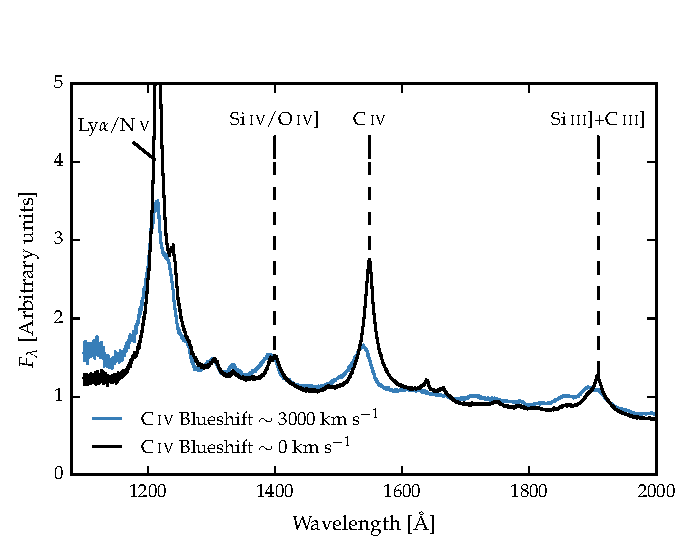
\includegraphics[width=\columnwidth]{figures/chapter03/blueshift_composite.pdf}
\caption[{Composite spectra from Ly$\alpha$ to \ion{C}{III}] for quasars with different \ion{C}{IV} blueshifts.}]{Composite spectra from Ly$\alpha$ to \ion{C}{III}] for quasars with different \ion{C}{IV} blueshifts. The systematic variation in the \ion{C}{IV} shape is correlated with changes in the quasar SEDs, including the strengths of the \ion{Si}{III}]$\lambda$$1892$ and \ion{C}{III}]$\lambda$$1908$ emission-lines.}
  \label{fig:blueshift_composite}
\end{figure}

Of potentially more significance for studies of BH masses as a function of quasar and host-galaxy properties are redshift errors that depend on the form of the quasar ultra-violet SED.
The systematic variation in the \ion{C}{IV} shape is correlated with changes in the quasar SEDs, including the strengths of the \ion{Si}{III}]$\lambda$$1892$ and \ion{C}{III}]$\lambda$$1908$ emission-lines in the rest-frame ultra-violet (Figure~\ref{fig:blueshift_composite}). 
As a consequence, the redshifts from \citet{hewett10} still suffer from systematic errors that are correlated with the shape, and particularly the blueshift, of the \ion{C}{IV} emission-line.
For the \citet{hewett10} redshifts, and ultra-violet emission-line based redshifts in general, quasars with large \ion{C}{IV} EQW and modest blueshifts have relatively small ($\simeq300$\,\kms) SED-dependent redshift errors.
Redshift uncertainties as large as $\simeq1000$\,\kms\, for such quasars are unusual and the large relative error in the corrected \ion{C}{IV} BH mass given in Table~\ref{tab:bhm_error} is pessimistic. 

Conversely, systematic redshift errors are greatest for quasars with large blueshifts, reaching $\sim750$\,\kms\, in the extreme for the \citet{hewett10} values. 
The associated error in the corrected \ion{C}{IV} BH masses is, however, mitigated somewhat due to the smaller gradient of the MBH(\ion{C}{IV})/MBH(Balmer) relation at large \ion{C}{IV} blueshift (see Figures~\ref{fig:correction_ha_b} and \ref{fig:correction_hb_b}). 
A definitive quantification of any systematic SED-dependent errors present in the quasar redshifts contained in the SDSS DR$12$ catalogue is not yet available but the principal component analysis (PCA) based redshift estimates are expected to be largely free of SED-dependent systematics. 

Using published redshift estimates, notably those from \citet{hewett10} for the SDSS DR$7$ quasars and the PCA-based redshifts from \citet{paris17} for SDSS DR$12$, the correction formula given in Section~\ref{sec:correction} produces significant improvements to \ion{C}{IV}-based BH mass estimates.
In a forthcoming work, Allen \& Hewett (2017, in preparation) will present a new redshift-estimation algorithm that produces redshifts independent of the \ion{C}{IV} blueshift and other variations in the ultra-violet SEDs of luminous quasars.
The low-ionization emission-lines visible in the rest-frame ultra-violet (over wavelengths from \ion{Mg}{II}$\lambda\lambda$$2796$,$2803$ down to the \ion{O}{I}$\lambda$$1304$+\ion{Si}{II}$\lambda$$1307$ blend) using the new redshift-algorithm are located at rest-frame wavelengths in excellent agreement with the systemic redshift defined using the rest-frame narrow-line optical [\ion{O}{III}] doublet and broad-line \hb and \hans.
SED-dependent systematic errors are below the apparent inherent dispersion of $\simeq220$\,\kms\, associated with broad emission-line redshifts \citep{shen16b}.

Figure~\ref{fig:civ_space_z_compare_c} shows the \ion{C}{IV} emission-line parameters calculated using the Allen \& Hewett redshift-estimation algorithm.  
The systematic trends seen in Figure~\ref{fig:civ_space_z_compare_b}, in particular the extension to high blueshift at low \ion{C}{IV} EQW, become more apparent in Figure~\ref{fig:civ_space_z_compare_c}, as expected from consideration of the known SED-related errors in the redshifts from \citet{hewett10}.
A population of quasars with only modest blueshifts and low EQW is also apparently still present. 

\subsubsection{\ion{C}{IV} emission-line blueshift measurements}
\label{sec:ch3-civmeasure}

The differences in the distribution of \ion{C}{IV} emission-line properties seen in the three panels of Figure~\ref{fig:civ_space_z_compare} are due primarily to the change in the systemic redshift estimates. 
It is also necessary, however, to obtain a measure of the \ion{C}{IV} emission-line `location' in order to calculate the blueshifts. 
When working with moderately-sized samples, parametric fits to the emission-line profile may be undertaken using careful mask-definition to minimise the effect of absorption features on the profiles used for the parametrisation, and this is the approach we followed in Section~\ref{sec:spec_measures}.

Effective analysis of the tens of thousands of spectra from SDSS DR$7$, and now DR$12$, however, requires a more robust scheme to determine a \ion{C}{IV}-blueshift estimate that is not very sensitive to the range of S/N among the spectra or the presence of narrow absorption systems within the \ion{C}{IV}-emission profile. 
\citet{shen11} provide a discussion (their section~3) of the factors that effect the measurement of broad emission-lines in quasar spectra of modest S/N. 
Their careful analysis of the \ion{C}{IV} emission properties employed the results of parametric fits of three Gaussians to the spectra. 

We take a different approach by adopting a non-parametric scheme to measure the blueshift of the \ion{C}{IV{}} line. 
The continuum is first modelled and subtracted using the procedure described in Section~\ref{sec:civ}. 
The \ion{C}{IV} emission-line is taken to lie within the wavelength interval $1500$-$1600$\,\AA. 
To reduce the impact of narrow absorption systems on the emission-line profile a `pseudo continuum' is defined by applying a $41$-pixel median filter to the quasar spectrum.
Pixels within the \ion{C}{IV} profile that lie more than $2$-$\sigma$ below the pseudo-continuum are deemed to be affected by absorption and added to an `absorber'-mask. 
Two pixels on either side of each such pixel are also included in the mask. 
For each masked pixel, the flux values in the spectrum are replaced by values from the pseudo-continuum\footnote{While the absorption identification and interpolation scheme is not effective for spectra that possess
associated absorption spread over more than $\sim1200$\,\kms, objects containing \ion{C}{IV} lines with such extensive absorption have been removed from the sample.}. 
The wavelength that bisects the cumulative total line flux is recorded and the blueshift computed using Equation~\ref{eq:civblueshift}. 

Our experiments in quantifying the \ion{C}{IV} emission properties of SDSS spectra show that this simple non-parametric measure of the \ion{C}{IV} emission location reduces the number of outliers significantly relative to the Gaussian-fitting scheme employed by \citet{shen11}. 
Visual inspection of spectra demonstrate that the improvement is due primarily to the identification of, and interpolation over, associated and outflow absorption systems.

\subsection{Systematic trends in residuals}
\label{sec:ch3-residuals}

The scatter about the best-fitting line in the FWHM(\ion{C}{IV})/FWHM(\hans) versus \ion{C}{IV}-blueshift relation is $\sim0.1$\,dex. 
With a view to reducing the scatter further, we searched for parameters which correlate with the scatter at fixed \ion{C}{IV} blueshift, including the luminosity, redshift, [\ion{O}{III}] EQW, and \ion{Fe}{II} EQW.
The only significant correlation we find is with the \ha FWHM (Figure~\ref{fig:residuals_ha_fwhm}).
Quasars with broad \ha lines tend to lie below the relation while quasars with narrow \ha tend to lie above it.
One possibility is that this correlation is simply due to random scatter (either intrinsic or measurement error) in the \ha FWHM which, with the other quasar properties fixed, would naturally produce a correlation between FWHM(\ion{C}{IV})/FWHM(\hans) and FWHM(\hans).
However, the fact that we see no such correlation between the model residuals and the \ion{C}{IV} FWHM suggests that the \ha FWHM correlation could be revealing something more fundamental. 
The \hans FWHM is part of the \citet{boroson92} EV$1$. 
Figure~\ref{fig:residuals_ha_fwhm} suggests that part of the scatter between the Balmer and \ion{C}{IV} velocity widths might be attributed to differences in the spectral properties which are correlated with EV$1$ \citep{marziani13}. 

\begin{figure}
    \centering 
    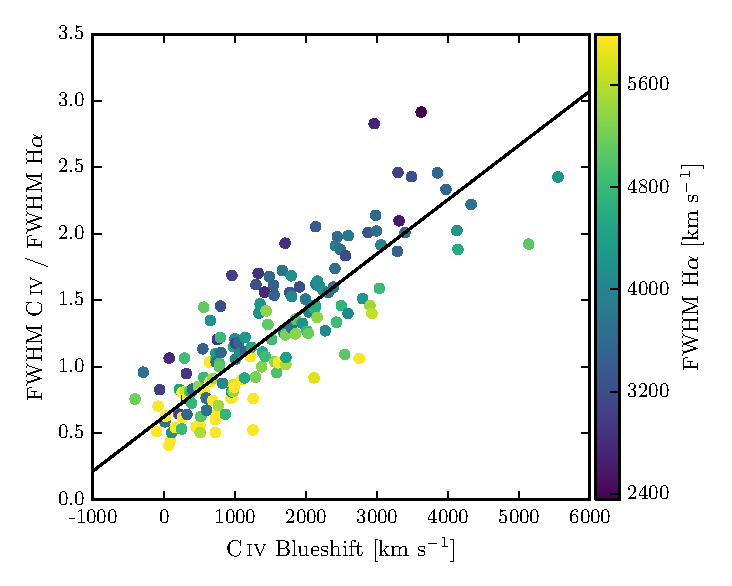
\includegraphics[width=0.8\textwidth]{figures/chapter03/fwhm_correction_color.pdf}  
    \caption[{Same as Figure~\ref{fig:correction_ha_a}, with the marker colour representing the \ha FWHM.}]{Same as Figure~\ref{fig:correction_ha_a}, with the marker colour representing the \ha FWHM. At fixed \ion{C}{IV} blueshift, there is a clear \ha FWHM dependent systematic in the model residuals.}   
    \label{fig:residuals_ha_fwhm}
\end{figure}


The shape of an emission-line can be characterised by the ratio FWHM/$\sigma$.  
FWHM/$\sigma$ $\simeq 2.35$ for a Gaussian profile, while FWHM/$\sigma$ $\simeq 1$ for a peakier Lorentzian profile\footnote{Strictly FWHM/$\sigma$ $\rightarrow 0$ for a Lorentzian profile, but values close to unity are typical when the dispersion is calculated over a velocity range, $\simeq\pm10\,000$\,\kms, used to parametrize broad emission-lines in quasar spectra.}.
In our sample, we find the model residuals and the \ha FWHM correlate with the shape of the line.   
The narrow lines are, on average, `peakier' (with FWHM/$\sigma\simeq1$) than the broader lines (with FWHM/$\sigma\simeq2$).   
This suggests that the BLR structure (e.g. the balance between rotation, turbulence and radial motions) is changing with the emission-line FWHM \citep[e.g.][]{collin06,kollatschny11,Kollatschny13}. 
This raises the question of whether the Balmer-line FWHM is a reliable proxy for the virial-induced velocity dispersion for the full range of Balmer line shapes we have in our sample. 

When calibrating the virial-product to masses derived independently using the $M_{\text{BH}}-\sigma$ relation, \citet{collin06} find that the scaling factor, $f$, is a factor $\sim2$ larger for their Population `$1$' sources (with FWHM/$\sigma < 2.35$ and essentially equivalent to population A of \citealt{sulentic00b}) than for their Population $2$ (with FWHM/$\sigma > 2.35$ and equivalent to population B of \citealt{sulentic00b}). 
For single-epoch BH mass estimates, assuming a constant value of the virial coefficient, $f$, as is normally done \citep[e.g.][]{vestergaard06}, means that Population $1$ masses will be underestimated and Population $2$ will be overestimated.
This could account for some of the remaining scatter between the \ion{C}{IV}- and Balmer-based BH masses (Figure~\ref{fig:residuals_ha_fwhm}). 

\citet{shen14} argue that a large part of the scatter observed in the \hb FWHM relates not to a spread in BH masses, but rather to the orientation of the BLR relative to the line-of-sight of the observer.
This would be the case if the BLR had a flattened disc-like geometry. 
In this case, the observed line width would increase with the inclination of the disc relative to the line of sight. 
At radio wavelengths, the morphology of the radio structure, parametrized in terms of `core dominance', is believed, at least in a statistical sense, to be a proxy for the orientation of the accretion disc \citep[e.g.][]{jackson91}.
Twenty core-dominated quasars and six lobe-dominated quasars were identified in our sample, but no statistically significant differences in the \ha line-widths of the two samples were found. 
It should be noted that the sub-sample of radio-detected quasars is small and the effectiveness of the test is further compromised by the lack of radio-detected quasars at large blueshifts \citep[see figure 14 of][for example]{richards11}.

\subsection{Effectiveness of the \ion{C}{IV} blueshift based correction to BH masses}
\label{sec:effectiveness}

\begin{figure}[t!]
    \centering
    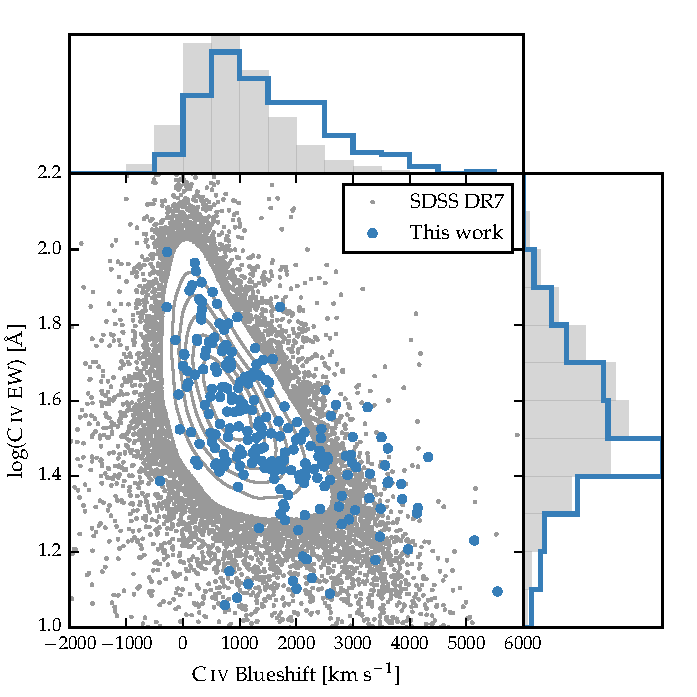
\includegraphics[width=0.9\textwidth]{figures/chapter03/civ_space.pdf} 
    \caption[{Rest-frame EQW versus blueshift of the broad \ion{C}{IV} emission-line for our sample and for SDSS quasars.}]{Rest-frame EQW versus blueshift of the broad \ion{C}{IV} emission-line for SDSS DR$7$ quasars and our sample (see Figure~\ref{fig:civ_space_z_compare_b} for details). Our sample has very good coverage of the parameter space; the shift to high blueshifts is a result of the high luminosity of our sample in relation to the SDSS sample and the correlation between luminosity and \ion{C}{IV} blueshift.} 
    \label{fig:civ_space}
\end{figure}

Figure~\ref{fig:civ_space} demonstrates that our sample has an excellent coverage of the \ion{C}{IV} EQW-blueshift parameter space in relation to SDSS DR$7$ quasars at redshifts $1.6 < z < 3.0$. 
The systematic offset to higher \ion{C}{IV} blueshifts for our catalogue relative to the SDSS quasars as a whole is a result of the higher mean luminosity relative to the SDSS sample (Figure~\ref{fig:lzplane}).
Our sample includes $21$ quasars with \ion{C}{IV} blueshifts $>3000$\,\kms, and extends to $\sim5000$\,\kms, i.e. at the very extreme of what is observed in this redshift and luminosity range. 
This demonstrates that the \ion{C}{IV}-blueshift based correction derived in this chapter is applicable to very high blueshifts. 
Conversely, there are no quasars in our catalogue with \ion{C}{IV} blueshifts $\lesssim0$\,\kms\, and we caution against extrapolating the correction formula to negative blueshifts.
In particular, quasars with negative blueshifts as large as $\sim1000$\,\kms\, appear in the SDSS DR$7$ catalogue and applying our correction in this regime boosts the derived masses by un-physical factors.    

\begin{figure}
    \captionsetup[subfigure]{labelformat=empty}  
    \centering 
    \subfloat[\label{fig:bhm_comparison_a}]{}
    \subfloat[\label{fig:bhm_comparison_b}]{}
    \subfloat[]{{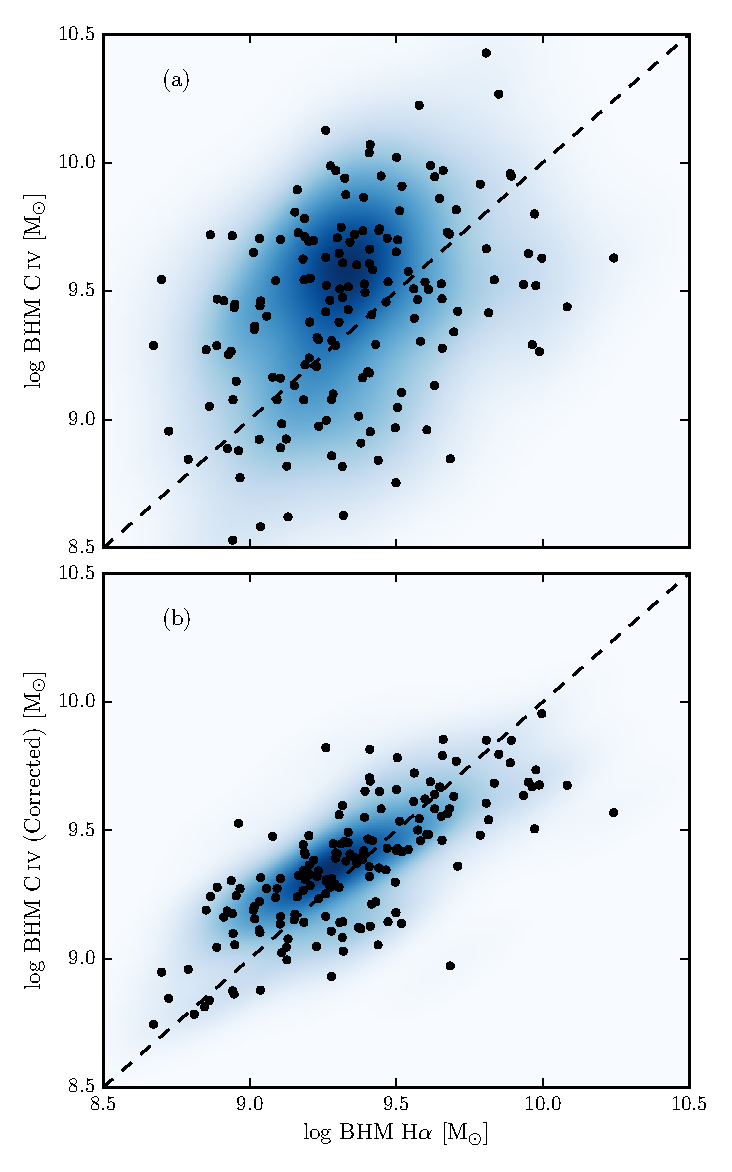
\includegraphics[width=0.8\textwidth]{figures/chapter03/bhm_comparison.pdf} }}
    \caption[{Comparison of the \ion{C}{IV}- and \hans-based BH masses before and after applying the \ion{C}{IV} blueshift-based correction to the \ion{C}{IV} FWHM.}]{Comparison of the \ion{C}{IV}- and \hans-based BH masses before (a) and after (b) applying the \ion{C}{IV} blueshift-based correction to the \ion{C}{IV} FWHM. The density of the plotted points (estimated using a Gaussian kernel density estimator) is represented by the colour. The correction to the \ion{C}{IV} BH masses decreases the scatter from $0.4$ to $0.2$\,dex.}   
    \label{fig:bhm_comparison}
\end{figure}

Figure~\ref{fig:bhm_comparison} compares the \ion{C}{IV}- and \hans-based BH masses before and after applying the blueshift-based correction to the \ion{C}{IV} FWHM.
Before the correction, the correlation between the \ion{C}{IV}- and \hans-based BH masses is very weak, and the scatter between the masses is $0.4$\,dex. 
After correcting the \ion{C}{IV} FWHM for the non-virial contribution, the correlation improves dramatically. 
The scatter between the corrected \ion{C}{IV}-based masses and the \hans-based masses is reduced to $0.2$\,dex. 
The scatter is $0.24$\,dex at low \ion{C}{IV} blueshifts ($\sim0$\,\kms) and $0.10$\,dex at high blueshifts ($\sim3000$\,\kms). 

\begin{figure}[h!]
    \centering 
    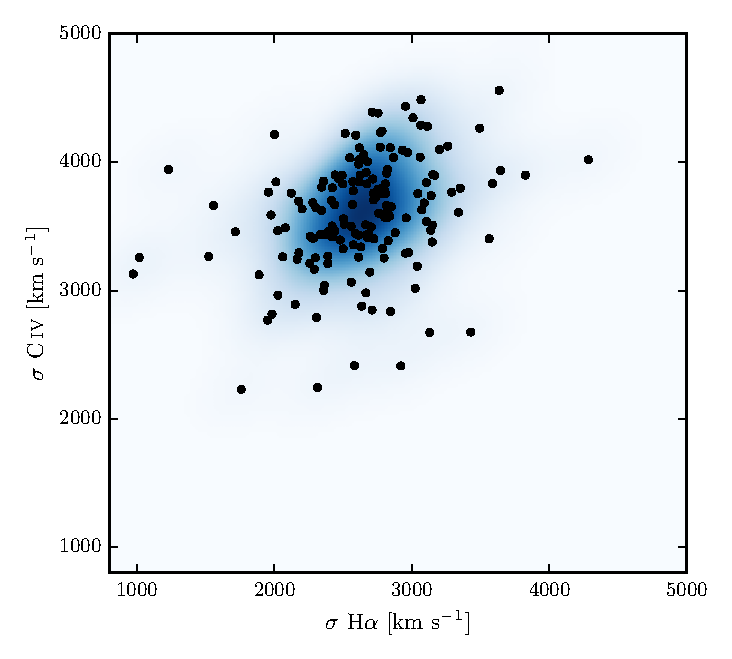
\includegraphics[width=0.8\columnwidth]{figures/chapter03/dispersion_comparison.pdf} 
    \caption[{Comparison of the \ion{C}{IV} and \ha line dispersion}]{Comparison of the \ion{C}{IV} and \ha line dispersion, $\sigma$. The density of the plotted points (estimated using a Gaussian kernel density estimator) is represented by the colour. Estimating a reliable BH mass from the \ion{C}{IV} FWHM and blueshift is substantially more effective than using the \ion{C}{IV} line dispersion with, or without, the line blueshift. The \ion{C}{IV} dispersion values are larger than the corresponding \ha measurements by a factor of $1.4$ on average, which is consistent with reverberation mapping measurements \citep{vestergaard06}.} 
    \label{fig:dispersion_comparison}
\end{figure}

There has been a considerable amount of attention regarding the relative merits of using the FWHM or dispersion to characterise the velocity width \citep[e.g.][]{denney13}.
The existence of a trend in the \ion{C}{IV}-dispersion values with \ion{C}{IV} blueshift is evident from inspection of Figure~\ref{fig:line_comparison_civ_b} but the systematic trend relative to the spread at fixed blueshift is significantly smaller than when using \ion{C}{IV} FWHM. 
Therefore, without the blueshift information, using the line dispersion would yield a more accurate BH mass than the FWHM (Figure~\ref{fig:dispersion_comparison}). 

The correlation between the \ha and \ion{C}{IV} line dispersion is, however, weak. 
The Pearson coefficient for the correlation is $0.36$ (and just $0.15$ when the \hb measurements are used in place of \hans). 
Furthermore, there is little dynamic range in the line dispersion: the scatter is just $480$ and $460$\,\kms\, for \ha and \ion{C}{IV} respectively. 
This observation suggests that the line dispersion does not fully trace the dynamic range in BH mass present in the quasar population. 
At least part of the reason is that the line dispersion is difficult to measure reliably in current survey-quality data, particularly because of the sensitivity to flux ascribed to the wings of the emission-line \citep[e.g.][]{mejia-restrepo16}.
Figures~\ref{fig:bhm_comparison} and \ref{fig:dispersion_comparison} demonstrate that estimating a reliable BH mass from the \ion{C}{IV} FWHM and blueshift is substantially more effective than using the \ion{C}{IV} line dispersion with, or without, the line blueshift. 

\subsection{Comparison to previous prescriptions}

\begin{figure}
    \captionsetup[subfigure]{labelformat=empty}
    \centering 
    \subfloat[\label{fig:compare_corrections_a}]{}
    \subfloat[\label{fig:compare_corrections_b}]{}
    \subfloat[\label{fig:compare_corrections_c}]{}
    \subfloat[]{{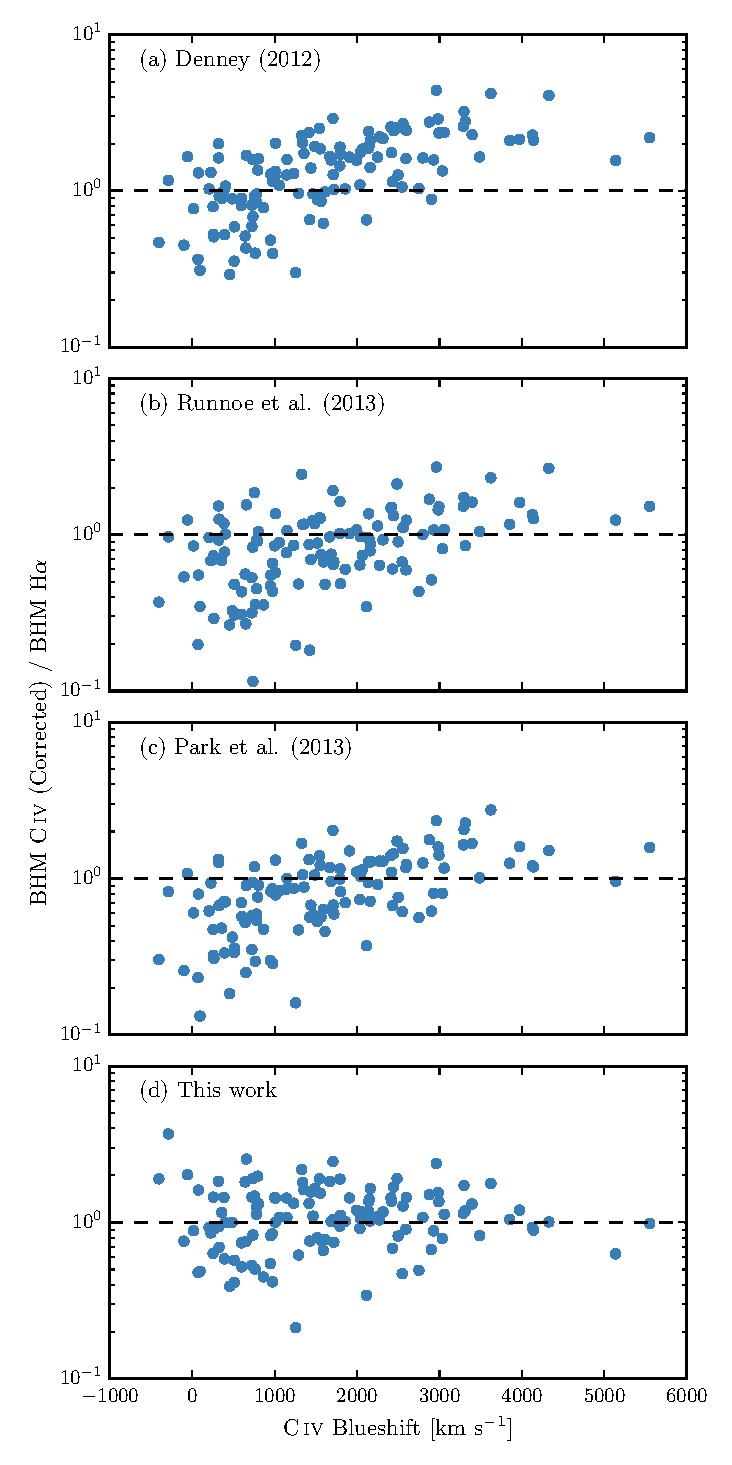
\includegraphics[width=0.9\textwidth]{figures/chapter03/corrections.pdf} }}
    \caption[{Comparison of BH mass estimates derived from \ion{C}{IV} and \ha as a function of the \ion{C}{IV} blueshift, using various corrections to the \ion{C}{IV}-based masses proposed in the literature.}]{Comparison of BH mass estimates derived from \ion{C}{IV} and \ha as a function of the \ion{C}{IV} blueshift. Corrections to the \ion{C}{IV}-based masses have been applied based on the shape (FWHM/$\sigma$) of the \ion{C}{IV} emission-line \citep[a;][]{denney12}, the peak flux ratio of the \ion{Si}{IV}+\ion{O}{IV} blend relative to \ion{C}{IV} \citep[b;][]{runnoe13}, and by significantly reducing the dependence of the derived BH mass on the \ion{C}{IV} velocity-width \citep[c;][]{park13}.}
    \label{fig:compare_corrections}
\end{figure}

\begin{figure}
    \centering 
    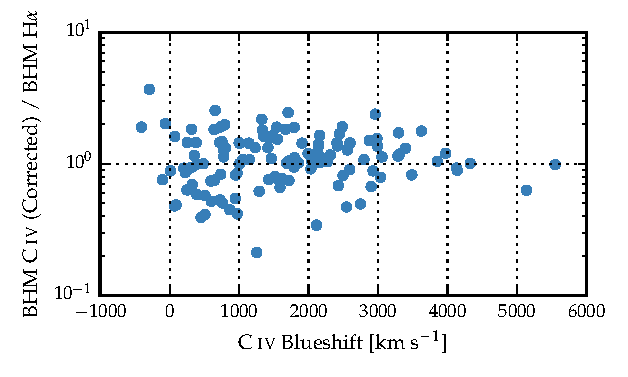
\includegraphics[width=0.9\textwidth]{figures/chapter03/corrections_coatman.pdf} 
    \caption[{Comparison of corrected \ion{C}{IV}-based BH masses and \hans-based masses as a function of the \ion{C}{IV} blueshift.}]{Comparison of BH mass estimates derived from \ion{C}{IV} and \ha as a function of the \ion{C}{IV} blueshift. \ion{C}{IV}-based masses have been corrected using the \ion{C}{IV} blueshift-based prescription presented in this chapter.}
    \label{fig:compare_corrections_coatman}
\end{figure}

In Figure~\ref{fig:compare_corrections} we compare various prescriptions which have been proposed in the literature to derive BH masses from the \ion{C}{IV} line which are consistent with the masses derived from the Balmer lines. 
In each case, we compare the corrected \ion{C}{IV}-based masses to the \hans-based masses as a function of the \ion{C}{IV} blueshift. 
The \ion{C}{IV} blueshift-based correction presented in this chapter is also tested in Figure~\ref{fig:compare_corrections_coatman}.
The correction proposed by \citet{runnoe13} is based on the spectral region at rest-frame wavelengths of $\sim$$1400$\,\AA\, (see below). 
Therefore, our analysis is based on the $123$ quasars with spectra covering this region. 

In Figure~\ref{fig:compare_corrections_a} the \ion{C}{IV} BH masses have been corrected using the \ion{C}{IV} shape (FWHM/$\sigma$) based correction proposed by \citet{denney12}. 
\citet{denney12} found the level of contamination in single-epoch spectra from non-reverberating gas to be correlated with the shape (FWHM/$\sigma$) of the \ion{C}{IV} profile. 
In our sample, we observe a strong correlation between the shape of the \ion{C}{IV} line and its blueshift (Figure~\ref{fig:line_comparison_civ_c}); between the two extremes in the \ion{C}{IV} blueshift distribution the line shape changes from FWHM/$\sigma\sim1-2.5$. 
The investigation of \citet{denney12} was based on a sample of reverberation mapped quasars, which have a narrow range of \ion{C}{IV} emission-line shapes, including the absence of any objects with large \ion{C}{IV} blueshifts. 
As a result, the correction is not applicable at large \ion{C}{IV} blueshifts. 
Therefore, while the consistency between the \hans- and \ion{C}{IV}-based masses at low \ion{C}{IV} blueshifts is improved, at high \ion{C}{IV} blueshifts the \ion{C}{IV}-based masses remain severely overestimated.

As explained above, reliably measuring the quasar systemic redshift from the ultra-violet region of the spectrum has proved difficult. 
However, the situation is improved dramatically by the new scheme developed by Allen \& Hewett (2017, in preparation). 
Given the difficulty of measuring reliable \ion{C}{IV} blueshifts without the Allen \& Hewett scheme, \citet{runnoe13} opted instead to use the continuum-subtracted peak flux ratio of the ultra-violet emission-line blend of \ion{Si}{IV}+\ion{O}{IV} (at $1400$\,\AA) to that of \ion{C}{IV} to correct for non-virial contributions to the \ion{C}{IV} velocity width. 
This parameter was chosen because it showed the strongest correlation with the FWHM \ion{C}{IV}/\hb residuals, as well as with the strengths of optical [\ion{O}{III}] and \ion{Fe}{II}. 

Following \citet{runnoe13}, we measure the peak flux by fitting a model with four Gaussian components (two for each emission-line) to the continuum-subtracted flux.
As is evident from Figure~\ref{fig:civ_space}, a correlation exists between the blueshift and EQW of \ion{C}{IV}: \ion{C}{IV} emission which is strongly blueshifted is typically weak. 
The \ion{Si}{IV}+\ion{O}{IV} emission-line blend, however, shows significantly less systematic variation (see Figure~\ref{fig:blueshift_composite}). 
Therefore, the \ion{Si}{IV}+\ion{O}{IV}-based correction is quite effective in practice: the systematic bias in the \ion{C}{IV} BH masses at large \ion{C}{IV} blueshifts is reduced to a factor of $\sim2$ (Figure~\ref{fig:compare_corrections_b}).
However, the \ion{C}{IV} based masses are still systematically overestimated at large \ion{C}{IV} blueshifts. 

In contrast to the widely-used \citet{vestergaard06} \ion{C}{IV}-based virial BH mass calibration, the more recent \citet{park13} calibration significantly reduces the dependence of the derived masses on the emission-line velocity width (from the $\Delta V^2$ dependence predicted assuming a virialized BLR to just $\Delta V^{0.56}$).
As a consequence, the \ion{C}{IV} based masses of the quasars with large \ion{C}{IV} blueshifts are much reduced (Figure~\ref{fig:compare_corrections_c}).
However, the systematic error in the \ion{C}{IV}-based BH masses as a function of \ion{C}{IV} blueshift remains. 

For comparison, the \ion{C}{IV}-based masses shown in Figure~\ref{fig:compare_corrections_coatman} have been corrected using the \ion{C}{IV} blueshift-based procedure presented in this chapter. 
No systematic in the BH masses as a function of the \ion{C}{IV} blueshift is evident. 

\section{Population trends with \ion{C}{IV} blueshift}
\label{sec:hatrends}

\begin{figure}
    \captionsetup[subfigure]{labelformat=empty}
    \centering 
    \subfloat[\label{fig:line_comparison_ha_a}]{}
    \subfloat[\label{fig:line_comparison_ha_b}]{}
    \subfloat[\label{fig:line_comparison_ha_c}]{}
    \subfloat[]{{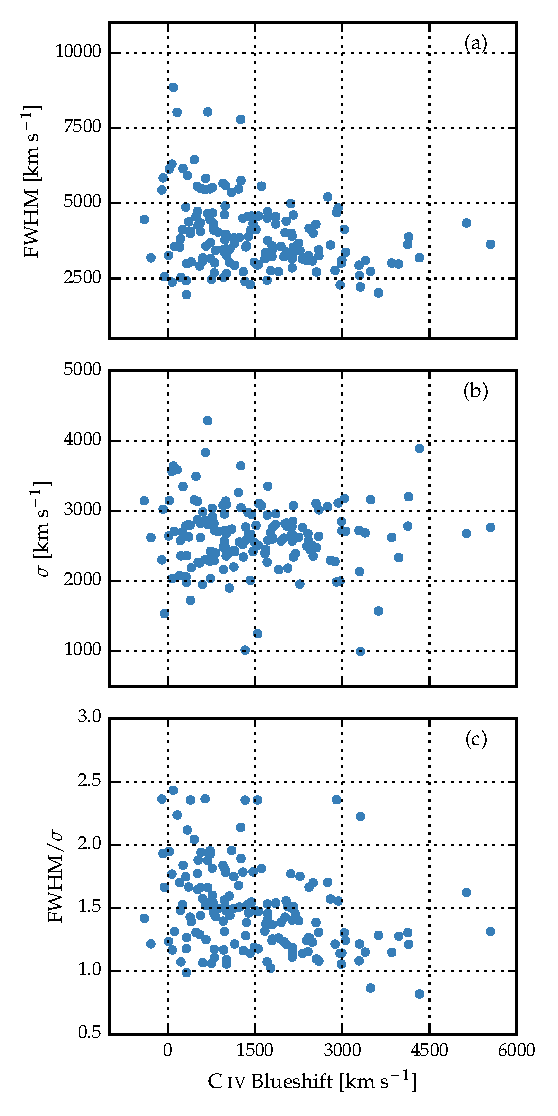
\includegraphics[width=0.8\textwidth]{figures/chapter03/ha_comparisons_paper2.pdf} }}
    \caption[{The FWHM, dispersion and shape of \ha as a function of the \ion{C}{IV} blueshift.}]{The FWHM, dispersion ($\sigma$) and shape (FWHM/$\sigma$) of \ha as a function of the \ion{C}{IV} blueshift.}
    \label{fig:line_comparison_ha}
\end{figure} 


\begin{figure}
    \centering
    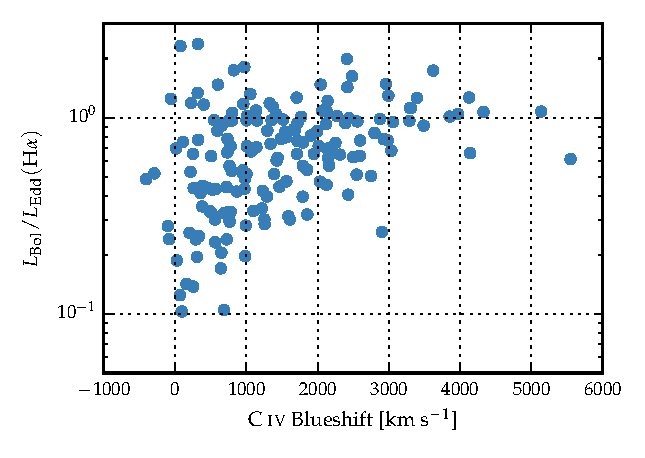
\includegraphics[width=0.8\linewidth]{figures/chapter03/ha_edd_civ_bs.pdf}
    \caption[{\hans-derived Eddington ratio versus \ion{C}{IV} blueshift.}]{\hans-derived Eddington ratio versus \ion{C}{IV} blueshift. At blueshift $\gtrsim2000$\,\kms\, all quasars have high accretion rates ($L/L_{\text{Edd}} \simeq 1$). This is in agreement with \citet{kratzer15}, but in contrast to what one would derive from naive use of \ion{C}{IV}-based BH mass scaling relations.}
    \label{fig:ha_edd_civ_bs}
\end{figure}

As shown in Figure~\ref{fig:line_comparison_ha}, there are systematic variations in the \ha line profile as a function of the \ion{C}{IV} blueshift. 
At \ion{C}{IV}-blueshift $<1200$\,\kms, the \ha FWHM range is $\simeq2000 - 8900$\,\kms, with mean $\simeq4300$\,\kms\, (Figure~\ref{fig:line_comparison_ha_a}). 
However, amongst the quasars with \ion{C}{IV}-blueshift $>2000$\,\kms, the mean \ha FWHM $=3500$\,\kms, with a scatter of just $700$\,\kms. 
There is also an apparent trend of peakier \hans-emission, with FWHM/$\sigma$ close to unity, at large \ion{C}{IV}-blueshift (Figure~\ref{fig:line_comparison_ha_c}). 
Amongst the low-\ion{C}{IV}-blueshift population there are in addition quasars with broader and more Gaussian-like \ha line profiles, with FWHM/$\sigma \simeq 2$ . 

The change in the \ha emission-line profiles as a function of \ion{C}{IV}-blueshift means that the \hans-FWHM derived BH masses at high-blueshift are smaller than the sample mean. 
We transformed the observed luminosity into a mass-normalised accretion rate (Eddington ratio).
To convert the monochromatic luminosity, which is observed, into a bolometric luminosity we use the bolometric correction factor given by \citet{richards06} ($L_{\text{Bol}} = 9.26L_{5100}$).
Although there is evidence that the bolometric correction factor is a function of the luminosity, as well as of other parameters including the \ion{C}{IV} blueshift \citep{krawczyk13}, the differences are small over the parameter range covered by our sample, and for simplicity we adopt a constant factor. 

The results, shown in Figure~\ref{fig:ha_edd_civ_bs}, demonstrate that at large blueshifts quasars are accreting at around their Eddington limits. 
This finding is in accord with our interpretation that the blueshifting of \ion{C}{IV} is evidence for strong outflows resulting from the presence of a radiation-driven accretion-disc wind. 
\citet{richards02} found that quasars with large \ion{C}{IV} blueshifts have weak \ion{He}{II}.
This is evidence for weak soft X-ray continuum emission \citep{leighly04}, which would allow a strong line-driven wind to form.  
The strength of such a wind is predicted to be related to the quasar far-ultra-violet SED, which, in turn, could be related to the mass-accretion rate.

All of the objects in our sample which exhibit large \ion{C}{IV} blueshifts would be classified as population A in the \citet{sulentic00b} scheme based on the \ha FWHM. 
Our results therefore support the idea of the \citet{sulentic00b} A/B division being driven by the Eddington ratio, with population A sources possessing higher accretion rates.
However, we also observe a number of quasars which have high Eddington ratios but do not have line profiles suggestive of strong outflows in the \ion{C}{IV} BLR.  
This suggests that a high accretion rate is a necessary but not sufficient condition for the existence of outflows \citep{baskin05}. 

The two-dimensional nature of the \ion{C}{IV} emission-line parametrisation and the apparent anti-correlation between \ion{C}{IV} EQW and \ion{C}{IV} blueshift suggests that the quasar population exhibits a continuum of properties. 
As such, more accurate \ion{C}{IV} blueshift measurements for SDSS-quasars should allow an improved mapping between the \ion{C}{IV}-emission properties and key physical parameters of the quasars.
This includes improving our understanding of the origin of quasars with exceptionally weak, blueshifted \ion{C}{IV} emission \citep[weak emission-line quasars;][]{luo15} which could be exotic versions of wind-dominated quasars \citep{plotkin15}.

As we described in Section~\ref{sec:ch3-residuals}, the shape of the Balmer lines (FWHM/$\sigma$) depends strongly on the FWHM. 
This suggests that the BLR structure is changing with the emission-line FWHM. 
One possibility we discussed is that the Balmer line-width is orientation-dependent \citep[e.g.][]{shen14}. 
This raises the question of whether the narrow \ha emission-lines observed in the quasars with the largest \ion{C}{IV} blueshifts could be an orientation effect. 
However, there is no evidence that the \ion{C}{IV} blueshift is dependent on the orientation \citep[inferred from the radio core-dominance;][]{richards11,runnoe14}. 
Furthermore, \citet{leighly04} showed that the \ion{He}{II}\l$1640$ emission-line properties of quasars with large \ion{C}{IV} blueshifts are more consistent with differences in the SED rather than differences in the orientation.
Overall, therefore, orientation does not appear to be the dominant effect in determining the \ion{C}{IV} blueshift and correlated changes in the \ha line profile.

As mentioned in Section~\ref{sec:ch3-intro} and discussed in \citet{richards11}, quasars with current reverberation mapping measurements have a restricted range of \ion{C}{IV}-line shapes. 
In particular, there are currently very few reverberation-mapping measurements of quasars with large \ion{C}{IV} blueshifts. 
Looking to the future, the results of the large on-going statistical reverberation mapping projects \citep[e.g.][]{shen15,kingoz15} for luminous quasars at high-redshift will shed new light on the Balmer line emitting region of the BLR for quasars with a range of \ion{C}{IV} blueshifts and lead to a greater understanding of the relation between the Balmer line profile and the BH mass.


\section{Frequency of quasars with high accretion rates}

Quantifying the frequency of quasars producing outflows as a function of key parameters, e.g. quasar luminosity, BH mass, redshift, etc. will be important to constrain models of quasar-galaxy evolution.  
At fixed BH mass, the intrinsic and the observed fraction of quasars exhibiting properties that depend on the Eddington ratio can differ significantly. 
As an illustration, we consider the implications for the intrinsic fraction of quasars possessing large \ion{C}{IV} blueshifts given the observed numbers in the $i<19.1$ flux-limited sub-sample of the SDSS DR$7$ quasar catalogue. 
In order to estimate the size of the selection effect, we considered the detection probability for a much-simplified quasar population. 
We assume that all quasars with \ion{C}{IV} blueshifts $>1200$\,\kms\, have enhanced accretion rates relative to the `normal' population (with \ion{C}{IV} blueshifts $<1200$\,\kms). 
If the accretion rate of the high-blueshift population is double the rate of the low-blueshift population (which is true in an average sense \---\ see Figure~\ref{fig:ha_edd_civ_bs}), then the high-blueshift population will be brighter by $\simeq0.75$ magnitude.
Under the assumption that the BH mass distribution is independent of the \ion{C}{IV} blueshift, the high-blueshift population will then be over-represented in a flux-limited sample.
To estimate the size of the bias, we need to know how many more quasars, at redshifts $2 < z < 2.5$, there are with $i<19.1+0.75=19.85$ relative to $i < 19.1$.
This is the fraction of the population which, as a consequence of having enhanced accretion rates, are boosted above the survey flux limit.    
The main colour-selected SDSS DR$7$ quasar catalogue extends only to $i= 19.1$ and, assuming the luminosity function is continuous\footnote{The luminosity function and number-counts vary only smoothly \citep[e.g.][]{ross13} for the magnitude and redshift range used here.} we thus use the number counts at $i < 19.1$ and $i < 18.35$, which differ by a factor of $\simeq 4$. 

At redshifts $2 < z <2.5$, there are $3,834$ quasars with \ion{C}{IV} blueshifts $<1200$\,\kms\, and $2,484$ with blueshifts $>1200$\,\kms\, in the SDSS DR$7$ $i < 19.1$ quasar sample, a ratio of $\sim$ $2$:$1$. 
The above calculation, although much idealised, suggests that the intrinsic fraction of high-blueshift quasars is a factor of four smaller than in the flux-limited sample (i.e. $\sim15$ per cent of the ultra-violet-selected non-BAL quasar population). 

\section{Summary}
\label{sec:conclusions}

The main results of this chapter are as follows: 

\begin{itemize}

\item We have analysed the spectra of $230$ high-luminosity ($10^{45.5}-10^{48}$\,\ergs), redshift $1.5 < z < 4.0$ quasars for which spectra of the Balmer emission-lines and the \ion{C}{IV} emission-line exist.
The large number of quasars in our spectroscopic catalogue and the wide range in \ion{C}{IV} blueshifts the quasars possess has allowed us to directly investigate biases in \ion{C}{IV}-based BH mass estimates which stem from non-virial contributions to the \ion{C}{IV} emission as a function of the \ion{C}{IV} blueshift, which, in turn, depends directly on the form of the quasar ultra-violet SEDs \citep{richards11}.

\item The \ion{C}{IV} emission-based BH masses are systematically in error by a factor of more than five at $3000$\,\kms\, in \ion{C}{IV} emission blueshift and the overestimate of the BH masses reaches a factor of $10$ for quasars exhibiting the most extreme blueshifts, $\gtrsim5000$\,\kms. 

\item We have derived an empirical correction formula for BH mass estimates based on the \ion{C}{IV} emission-line FWHM and blueshift.
The correction may be applied using Equations~\ref{eq:hafwhm} and \ref{eq:masscorrection} in Section~\ref{sec:correction}.
The large SED-dependent systematic error in \ion{C}{IV}-based BH masses is removed using the correction formulae.
The remaining scatter between the corrected \ion{C}{IV}-based masses and the \hans-based masses is $0.24$\,dex at low \ion{C}{IV} blueshifts ($\sim0$\,\kms) and $0.10$\,dex at high blueshifts ($\sim3000$\,\kms). 
This is a significant improvement on the $0.40$\,dex scatter observed between the un-corrected \ion{C}{IV} and \ha BH masses. 
The correction depends only on the \ion{C}{IV} line properties -- i.e. the FWHM and blueshift -- and allows un-biased single-epoch virial BH mass estimates to be made from optical spectra, such as those provided by the SDSS, out to redshifts exceeding $z\sim 5$. 

\end{itemize}

\section{Catalogue of derived properties}

Table~\ref{tab:bhm-specmeasure} includes the line parameters from our emission-line fits, and other derived properties used in this chapter. 
The columns in Table~\ref{tab:bhm-specmeasure} are as follows:

\begin{itemize}

 \item[1] Catalogue name.

 \item[2-3] Broad \ha FWHM, and its error, in \kms.

 \item[4-5] Broad \ha line dispersion, and its error, in \kms.

 \item[6-7] Broad \ha redshift, and its error. 

 \item[8-9] \hans-FWHM-based BH mass using \citet{vestergaard06} calibration, and its error, in M$_\odot$. \ha FWHM is first converted into equivalent \hb FWHM using Equation~\ref{eq:ha2hb}. 

 \item[10-11] Broad \hb FWHM, and its error, in \kms.

 \item[12-13] Broad \hb line dispersion, and its error, in \kms.

 \item[14-15] Broad \hb redshift, and its error. 

 \item[16-17] \hbns-FWHM-based BH mass using \citet{vestergaard06} calibration, and its error, in M$_\odot$.  

 \item[18-19] Broad \ion{C}{IV} FWHM, and its error, in \kms.

 \item[20-1] Broad \ion{C}{IV} line dispersion, and its error, in \kms.

 \item[22-23] Broad \ion{C}{IV} EQW, and its error, in \AA.

 \item[24] \ion{Si}{IV}+\ion{O}{IV}/\ion{C}{IV} peak flux ratio.

 \item[25-27] \ion{C}{IV} blueshift, relative to \hans, and its error, in \kms.

 \item[27-28] \ion{C}{IV} blueshift, relative to \hbns, and its error, in \kms.

 \item[29-30] Uncorrected \ion{C}{IV}-FWHM-based BH mass using \citet{vestergaard06} calibration, and its error.

 \item[31] Corrected \ion{C}{IV}-FWHM-based BH mass.

\end{itemize}


\begin{table}
  \footnotesize 
  \centering
   \begin{tabular}{cccc} 
    \hline
    Column & Name & Units & Description \\ 
    \hline
    1  & UID & & Catalogue name \\
    2  & FWHM\_BROAD\_HA & \kms & Broad \ha FWHM \\ 
    3  & FWHM\_BROAD\_HA\_ERR & \kms & \\
    4  & SIGMA\_BROAD\_HA & \kms & Broad \ha $\sigma$\\
    5  & SIGMA\_BROAD\_HA\_ERR & \kms &\\
    6  & Z\_BROAD\_HA & & \ha redshift \\
    7  & Z\_BROAD\_HA\_ERR & &  \\
    8  & LOGMBH\_HA & M$_\odot$ & \ha BH mass\\ 
    9  & LOGMBH\_HA\_ERR & M$_\odot$ & \\ 
    10 & FWHM\_BROAD\_HB & \kms & Broad \hb FWHM\\
    11 & FWHM\_BROAD\_HB\_ERR & \kms & \\
    12 & SIGMA\_BROAD\_HB & \kms & Broad \hb $\sigma$ \\
    13 & SIGMA\_BROAD\_HB\_ERR & \kms & \\
    14 & Z\_BROAD\_HB & & \hb redshift\\
    15 & Z\_BROAD\_HB\_ERR & & \\
    16 & LOGMBH\_HB & M$_\odot$ & \hb BH mass \\ 
    17 & LOGMBH\_HB\_ERR & M$_\odot$ & \\ 
    18 & FWHM\_CIV & \kms & Broad \ion{C}{IV} FWHM \\
    19 & FWHM\_CIV\_ERR & \kms & \\
    20 & SIGMA\_CIV & \kms & Broad \ion{C}{IV} $\sigma$ \\
    21 & SIGMA\_CIV\_ERR & \kms & \\
    22 & EQW\_CIV & \AA & Broad \ion{C}{IV} EQW \\  
    23 & EQW\_CIV\_ERR & \AA & \\ 
    24 & $1400$\_CIV & & \ion{Si}{IV}+\ion{O}{IV}/\ion{C}{IV} peak flux ratio \\ 
    25 & BLUESHIFT\_CIV\_HA & \kms & \ion{C}{IV} blueshift, relative to \hans \\
    26 & BLUESHIFT\_CIV\_HA\_ERR & \kms & \\
    27 & BLUESHIFT\_CIV\_HB & \kms & \ion{C}{IV} blueshift, relative to \hbns \\
    28 & BLUESHIFT\_CIV\_HB\_ERR & \kms & \\
    29 & LOGMBH\_CIV\_VP$06$ & M$_\odot$ & Uncorrected \ion{C}{IV} BH mass \\  
    30 & LOGMBH\_CIV\_VP$06$\_ERR & M$_\odot$ & \\ 
    31 & LOGMBH\_CIV\_C$17$ & M$_\odot$ & Corrected \ion{C}{IV} BH mass \\ 
    \hline
    \end{tabular}
    \caption[{The format of the table containing the emission-line properties from our parametric model fits.}]{The format of the table containing the emission-line properties from our parametric model fits and other derived parameters used in this chapter. The full table is available online at http://dx.doi.org/10.5281/zenodo.557069.}
  \label{tab:bhm-specmeasure}
\end{table}



% % !TEX root = ../main.tex

%************************************************
\chapter{Quasar-driven outflows of ionised gas}
\label{ch:nlr} 
%************************************************

\section{[\ion{O}{III}] as a probe of quasar-driven outflows}

X-ray and ultra-violet spectroscopy has revealed high-velocity outflows to be nearly ubiquitous in high accretion rate quasars.
Strong evidence for high-velocity outflows in the vicinity of quasars include BALs, NALs and blueshifted emission-lines. 
These observations suggest that the energy released by quasars can have a dramatic effect on their immediate environments. 

Quasars driving powerful outflows over galactic scales is a central tenet of galaxy evolution models involving `quasar feedback' \citep[e.g.][]{silk98,springel05,bower06}.
In recent years, a huge amount of resources have been devoted to searching for observational evidence of this phenomenon.  
This has resulted in recent detections of outflows in quasar-host galaxies using tracers of atomic, molecular, and ionised gas \citep[e.g.][]{nesvadba06,arav08,nesvadba08,moe09,alexander10,dunn10,feruglio10,nesvadba10,alatalo11,cano-diaz12,harrison12,harrison14,cimatti13,rupke13,veilleux13,cicone14,nardini15}.  

One particularly successful technique has been to use forbidden quasar emission-lines to probe the dynamical state of the ionised gas in quasar host-galaxies. 
Forbidden lines are suppressed by collisional de-excitation in higher-density environments and therefore, even in the absence of direct spatial information, [\ion{O}{III}] gas is assumed to be extended over kilo-parsec scales in luminous quasars. 
Because of its high equivalent width, [\ion{O}{III}]\l$5008$ is the most studied of the narrow quasar emission-lines. 
The [\ion{O}{III}] emission is found to consist of two distinct components: a narrow, `core' component, with a velocity close to the systemic redshift of the host-galaxy, and a broader `wing' component, which is normally blueshifted. 
The core component is dominated by the gravitational potential of the host-galaxy.
However, the velocity-width of the wing is much too broad for the gas to be in dynamical equilibrium with the host-galaxy \citep[e.g.][]{liu13} and the general consensus is that it is tracing high-velocity outflowing gas. The receding side of the outflow may be obscured due to the presence of dust, either in the outflow or elsewhere, and so only the near-side of the outflow, which is blueshifted, is observed. 
The relative balance between the core and wing components varies significantly from object to object, and governs the width and asymmetry of the overall [\ion{O}{III}] emission profile \citep[e.g.][]{shen14}. 

Observations of broad velocity-widths and blueshifts in narrow emission-lines stretch back several decades \citep[e.g.][]{weedman70,stockton76,heckman81,veron81,feldman82,heckman84,vrtilek85,whittle85,boroson92}. 
However, these studies rely on small samples, which are often unrepresentative of the properties of the quasar population. 
More recently, the advent of large optical spectroscopic surveys (e.g. SDSS) have facilitated studies of the NLR in tens of thousands of quasars \citep[e.g.][]{boroson05,greene05a,zhang11,mullaney13,zakamska14,shen14}. 
This has provided constraints on the prevalence and drivers of ionised outflows.   
At the same time, there is strong evidence from spatially resolved spectroscopy that these outflows are extended over galaxy scales \citep[e.g.][]{greene09,greene11,harrison12,hainline13,harrison14}. 

However, these studies do not cover the redshift range when star formation and BH accretion peaked ($2 \lesssim z \lesssim 4$), which is when the $M_{\mathrm BH}-\sigma$ relation is thought to have been established. 
At these redshifts bright optical emission-lines including the [\ion{O}{III}] doublet are redshifted to near-infrared wavelengths, where observations are far more challenging. 
As a consequence, studies at high redshifts have typically relied on relatively small numbers of objects.
These studies find [\ion{O}{III}] to be broader in more luminous quasars, with velocity-widths $\gtrsim1000$\,\kms\, common \citep[e.g.][]{netzer04,kim13,brusa15,shen16a}.  
These findings suggest that quasar efficiency in driving galaxy-wide outflows increases with luminosity \citep[e.g.][]{netzer04,nesvadba08,kim13,brusa15,carniani15,perna15,bischetti16}. 
The fraction of objects with very weak [\ion{O}{III}] emission also appears to increase with redshift and/or luminosity \citep[e.g.][]{netzer04}. 

In this chapter, we analyse the [\ion{O}{III}] properties of a sample of $354$ high-luminosity, redshift $1.5 < z < 4$ quasars.
To date, this is the largest study of the NLR properties of high redshift quasars. 

\section{Constructing a sample with [\ion{O}{III}] spectra}

From our near-infrared spectroscopic catalogue (Chapter~\ref{ch:nirsample}), we have selected $354$ quasars which have spectra covering the [\ion{O}{III}] doublet. 
The broad Balmer \hb line has also been observed for all but two of the sample. 
For $165$ quasars, the spectra extend to the broad \ha emission-line at $6565$\,\AA, and in $260$ objects optical spectra, including \ion{C}{IV}, are also available (mostly from SDSS/BOSS). 
The sample covers a wide range in redshifts ($1.5 \lesssim z \lesssim 4$) and luminosities ($45.5 \lesssim \log L_{\mathrm Bol} \lesssim 49$\,\ergs). 
The spectrographs and telescopes used to obtain the near-infrared spectra are summarised in Table~\ref{tab:specnums_ch4}.

\begin{table}
  \centering
  \footnotesize 
  \caption{The numbers of quasars with [\ion{O}{III}] line measurements and the spectrographs and telescopes used to obtain the near-infrared spectra.}
  \label{tab:specnums_ch4}
    \begin{tabular}{ccc} 
    \hline
    Spectrograph & Telescope & Number \\
                 &           & \\
    \hline
    FIRE         & MAGELLAN  & $31$ \\
    GNIRS        & GEMINI-N  & $28$ \\
    ISAAC        & VLT       & $7$ \\
    LIRIS        & WHT       & $7$ \\
    NIRI         & GEMINI-N  & $29$ \\
    NIRSPEC      & Keck II   & $3$ \\
    SINFONI      & VLT       & $80$ \\
    SOFI         & NTT       & $76$ \\
    TRIPLESPEC   & ARC-$3.5$m  & $27$ \\
    TRIPLESPEC   & P$200$      & $45$ \\
    XSHOOTER     & VLT       & $21$ \\
    \hline
    \multicolumn{2}{c}{Total} & $354$ \\
    \hline
    \end{tabular}
\end{table} 

\section{Spectral measurements}

In this section, we describe how emission-line parameters are derived. 
Our approach is to model the spectra using a power-law continuum, an empirical \ion{Fe}{II} template (taken from \citealt{boroson92}) and multiple Gaussian emission components.
Non-parametric properties are then derived from the best-fitting model. 
This approach, which is commonly adopted in the literature \citep[e.g.][]{shen11,shen12,shen16a}, is more robust when analysing spectra with limited S/N (in comparison to measuring line properties directly from the data) and allows adjacent emission-lines to be de-blended.

The same approach was used to model the \hbns/[\ion{O}{III}] complex in Chapter~\ref{ch:bhmass}. 
However, a number of small adjustments have been made to the model. 
\ha emission-line properties (used to estimate the quasar systemic redshift) are also re-derived in this chapter using a slightly modified model to the one adopted in Chapter~\ref{ch:bhmass}. 
\ion{C}{IV} emission-line properties (used to infer the strength of BLR outflows) are taken directly from Chapter~\ref{ch:bhmass}. 

\subsection{Transforming spectra to rest-frame wavelengths}

Before a spectrum can be modelled, it must first be transformed to the rest-frame of the quasar.  
The redshift used in this transformation is either derived from the peak of the broad \ha emission ($\sim40$ per cent of our sample), from the peak of the broad \hb emission ($\sim40$ per cent) or from the peak of the narrow [\ion{O}{III}] emission ($20$ per cent).
The rest-frame transformation is only required to be accurate to within $\sim1000$\,\kms\, of the true systemic redshift for our fitting procedure to function. 
In later sections, more precise estimates of the systemic redshift will be calculated using our parametric model fits. 

\subsection{Removing \ion{Fe}{II} emission}
\label{sec:ch4-fe-removal}

\begin{figure}
    \centering
    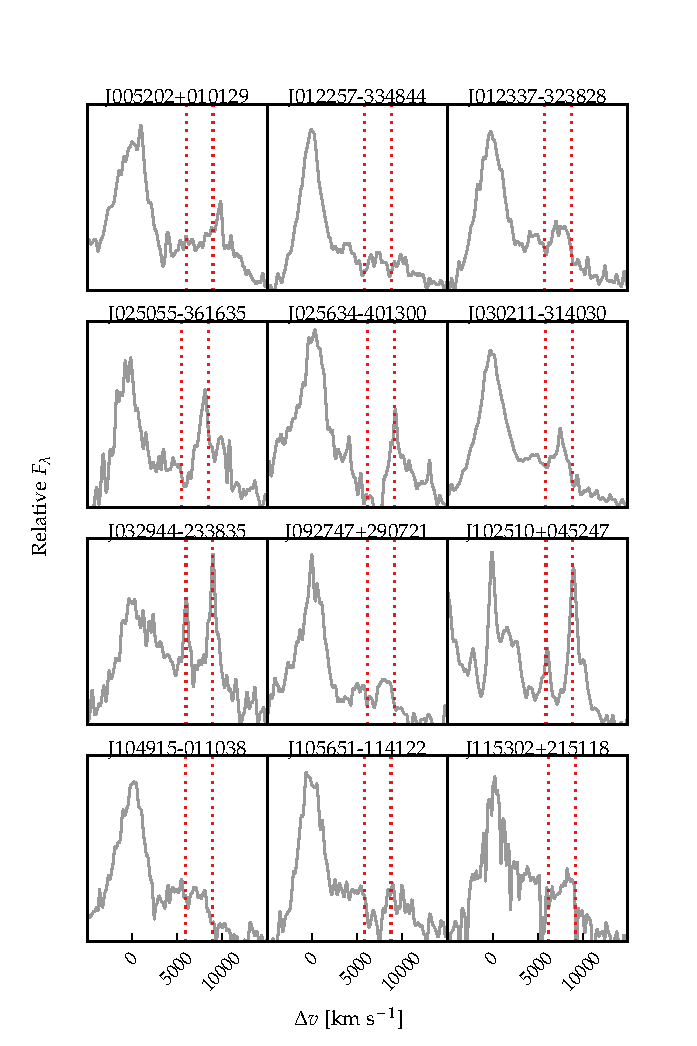
\includegraphics[width=\columnwidth]{figures/chapter04/example_spectrum_grid_extreme_fe_1.pdf} 
    \caption[{Spectra of the $24$ objects for which significant \ion{Fe}{II} emission is still present following our \ion{Fe}{II}-subtraction procedure.}]{Spectra of the $24$ objects for which significant \ion{Fe}{II} emission is still present following our \ion{Fe}{II}-subtraction procedure. Spectra have been smoothed via convolution with a $100$\,\kms\, Gaussian kernel. The vertical lines indicate the expected positions of the [\ion{O}{III}] doublet (which is generally very weak in these objects) with the systemic redshift defined using the peak of the broad \hb emission.}     
    \label{fig:bad_fe}
\end{figure}

\begin{figure}
\ContinuedFloat
    \centering
    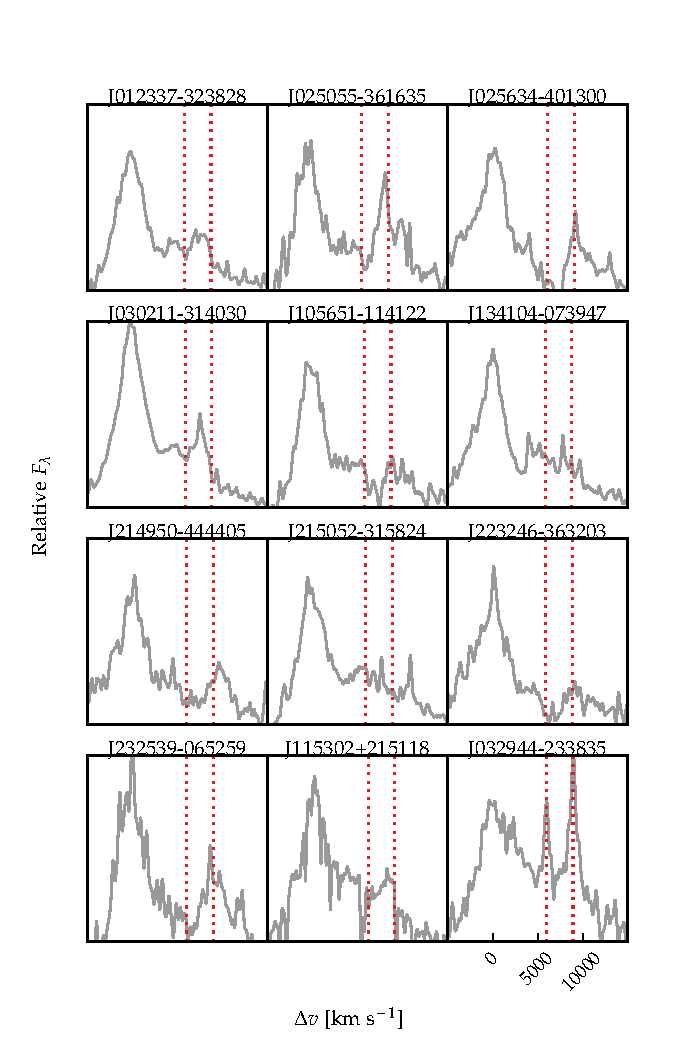
\includegraphics[width=\columnwidth]{figures/chapter04/example_spectrum_grid_extreme_fe_2.pdf} 
    \caption[]{Continued.}     
\end{figure}

Before \hbns/[\ion{O}{III}] is modelled, we first model and subtract the nearby continuum and \ion{Fe}{II} emission using the procedure described in Chapter~\ref{ch:bhmass}. 
We encountered $24$ objects for which the procedure failed to adequately remove the \ion{Fe}{II} emission from the spectra (Figure~\ref{fig:bad_fe}).  
In these objects the relative strengths of the \ion{Fe}{II} lines differ significantly from those of I Zw $1$, on which the \citet{boroson92} \ion{Fe}{II} template we use is based. 
The residual \ion{Fe}{II} emission is at rest-frame wavelengths very close to the laboratory wavelengths of the [\ion{O}{III}] doublet, which is generally very weak in these objects. 
As a result, the [\ion{O}{III}] line parameters we derive for these objects are unreliable. 
These objects are therefore flagged and excluded from our analysis in the remainder of this chapter (leaving $330$ objects in our sample). 

To illustrate the importance of the \ion{Fe}{II} subtraction procedure in reliably measuring [\ion{O}{III}] emission properties, we consider the object J$223819$-$092106$ (shown bottom row, centre in Figure~\ref{fig:bad_fe}). 
This object was also analysed by \citet{shen16a}, who reported the [\ion{O}{III}] emission to have an extreme redshift ($\sim7500$\,\kms) relative to the \citet{hewett10} systemic redshift.
However, our analysis suggests that the emission which was modelled by \citet{shen16a} as [\ion{O}{III}] is more likely to be poorly-subtracted \ion{Fe}{II}.  

\subsection{Modelling \hbns/[\ion{O}{III}]}
\label{sec:oiiimodel}

\begin{table}
  \centering
  \footnotesize 
  \caption{Summary of models used to fit the \hb emission, and the number of quasars each model is applied to.}
  \label{tab:hbmod}
    \begin{tabular}{ccc} 
    \hline
    Model & Fix centroids? & Number \\
    \hline
    $2$ broad Gaussians + $1$ narrow Gaussian & No & $9$ \\
    $2$ broad Gaussians & No  &  $295$ \\
    $2$ broad Gaussians & Yes &  $39$ \\
    $1$ broad Gaussian  & N/A &  $9$ \\
    \hline
    \end{tabular}
\end{table} 

In general, \hb is modelled with two Gaussians with non-negative amplitudes and FWHM greater than $1200$\,\kms.
In nine objects \hb is modelled with a single Gaussian and in $39$ objects \hb is modelled with two Gaussians, but the velocity centroids of the two Gaussians are constrained to be equal. 
These spectra generally have low S/N, and adding extra freedom to the model does not significantly decrease the  reduced-$\chi^2$.
In addition there are cases where the blue wing of the \hb emission is below the lower wavelength limit of the spectra; in these cases models with more freedom are insufficiently constrained by the data.    

Contributions to the \hb emission from the NLR is generally weak in our sample, and an additional Gaussian component to model this emission is not required for the vast majority of objects. 
In nine objects features in the model - data residuals suggest that a narrow emission component is significant, and an additional narrow Gaussian is included in the model for these quasars. 
If the NLR contribution to the \hb emission is significant in more of our sample, then measures of the \hb velocity-width will be biased to lower values. 
However, our systemic redshift estimates that use the peak of the \hb emission (Section~\ref{sec:ch4_redshifts}) will not be affected. 
The \hb models, and the numbers of quasars each model is applied to, are summarised in Table~\ref{tab:hbmod}. 

Each component of the [\ion{O}{III}] doublet is fit with one or two Gaussians, depending on the fractional reduced-$\chi^2$ difference between the one- and two-component models. 
Concretely, if the addition of the second Gaussian decreases the reduced-$\chi^2$ by more than $5$ per cent then the double-Gaussian model is accepted.
One hundred and twenty-eight spectra are fit with a single Gaussian and $140$ with two Gaussians. 
The peak flux ratio of the [\ion{O}{III}] $4960$\,\AA\, and $5008$\,\AA\, components are fixed at the expected $1$:$3$ ratio and the width and velocity offsets are set to be equal\footnote{For J$003136$+$003421$, a significantly better fit ($\Delta \chi^2_{\nu} \sim 25\%$) is obtained when the peak flux ratio constraint relaxed; the peak ratio of the best-fitting model is $1$:$2.13$.}.

In $62$ objects with very weak [\ion{O}{III}] (mean ${\mathrm EQW}\sim2$\,\AA) we find that the Gaussian model has a tendency to fit features to the noise. 
This can lead to large errors on the [\ion{O}{III}] line properties. 
To avoid this problem, we instead fit a fixed [\ion{O}{III}] template to the spectra, with the normalisation of this template the only free-parameter in the fit.
This template is generated by running our line-fitting routine on a median composite spectrum that we have constructed from the $268$ quasars with reliable [\ion{O}{III}] line measurements.  
The spectra used to construct the composite were first de-redshifted and continuum- and \ion{Fe}{II}-subtracted.  

The models we use to fit [\ion{O}{III}], and the numbers of quasars each model is applied to, are summarised in Table~\ref{tab:oiiimod}.

\begin{table}
  \centering
  \footnotesize 
  \caption{Summary of models used to fit the [\ion{O}{III}] emission, and the number of quasars each model is applied to.}
  \label{tab:oiiimod}
    \begin{tabular}{cc} 
    \hline
    Model & Number \\
    \hline
    $2$ Gaussians &  $140$ \\
    $1$ Gaussian  &  $128$ \\
    Template &  $62$ \\
    \hline
    \end{tabular}
\end{table} 

In Figure~\ref{fig:example_spectrum_grid} we show example fits to eight objects. 
The median reduced-$\chi^2$ value in the whole sample is $1.31$ and, in general, there are no strong features observable in the spectrum-minus-model residuals.

\begin{figure}
    \centering
    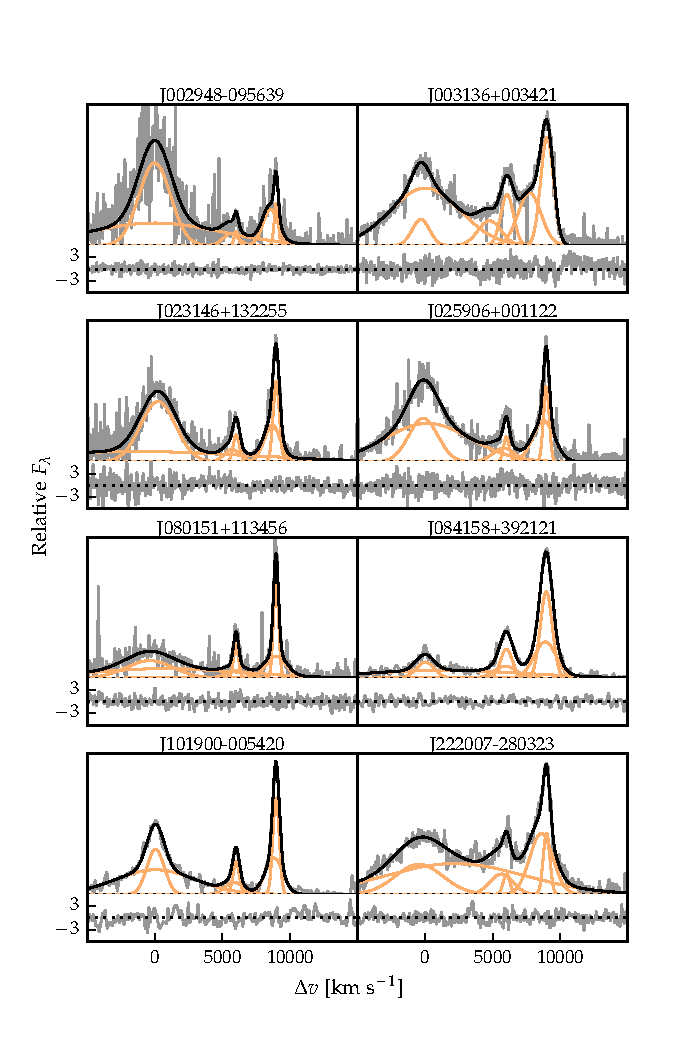
\includegraphics[width=\textwidth]{figures/chapter04/example_spectrum_grid.pdf} 
    \caption[{Model fits to the continuum- and \ion{Fe}{II}-subtracted \hbns/[\ion{O}{III}] emission in eight quasars.}]{Example model fits to the continuum- and \ion{Fe}{II}-subtracted \hbns/[\ion{O}{III}] emission in eight quasars. The data is shown in grey, the best-fitting model in black, and the individual model components in orange. The peak of the [\ion{O}{III}] emission is used to set the redshift, and $\Delta{v}$ is the velocity shift from the rest-frame transition wavelength of \hbns. Below each spectrum we plot the data-minus-model residuals, scaled by the errors on the fluxes.}     
    \label{fig:example_spectrum_grid}
\end{figure}

\subsection{Modelling \hans}
\label{sec:hamodel}

\begin{table}
  \centering
  \footnotesize 
  \caption{Summary of models used to fit the \ha emission, and the number of quasars each model is applied to.}
  \label{tab:hamod}
    \begin{tabular}{cccc} 
    \hline
    Model     & Components & Fix centroids? & Number \\
    \hline
    1        & $1$ broad Gaussian  & N/A &  $8$ \\
    2        & $2$ broad Gaussians & Yes &  $47$ \\
    3        & $2$ broad Gaussians & No  &  $20$ \\
    4        & $2$ broad Gaussians + narrow Gaussians & Yes & $42$ \\
    5        & $2$ broad Gaussians + narrow Gaussians & No  & $48$ \\
    \hline
    \end{tabular}
\end{table} 

There are $165$ quasars in our sample with spectra covering the \ha emission-line. 
In Section~\ref{sec:ch4_redshifts}, we use the peak of the \ha emission as one estimate of the quasar systemic redshift. 
In this section, we describe how the \ha emission was modelled. 

The continuum emission is first modeled and subtracted using the procedure described in Section~\ref{sec:ha}. 
We then test five different models with increasing degrees of freedom to model the \ha emission. 
The models are summarised in Table~\ref{tab:hamod}. 
They are (1) a single broad Gaussian; (2) two broad Gaussians with identical velocity centroids; (3) two broad Gaussians with different velocity centroids; (4) two broad Gaussians with identical velocity centroids, and additional narrower Gaussians to model narrow \ha emission, and the narrow components of [\ion{N}{II}]\ll$6548,6584$ and [\ion{S}{II}]\ll$6717,6731$; (5) two broad Gaussians with different velocity centroids, and additional narrower Gaussians. 
If used, the width and velocity of all narrow components are set to be equal in the fit, and the relative flux ratio of the two [\ion{N}{II}] components is fixed at the expected value of $2.96$.

In order to determine which model is selected for each spectrum we use the following procedure.  
Each of the five models are fit to every spectrum and the reduced-$\chi^2$ recorded.
Initially, the model with the smallest reduced-$\chi^2$ is selected. 
We then measure how the reduced-$\chi^2$ changes as the complexity of the model is decreased (i.e. considering the models in Table~\ref{tab:hamod} in descending order). 
If it results in an increase in the reduced-$\chi^2$ which is less than $10$ per cent relative to the best fitting model, then the simpler model is selected.  

\subsection{Deriving emission-line properties from the best-fitting models}

\begin{figure}[t!]
    \centering
    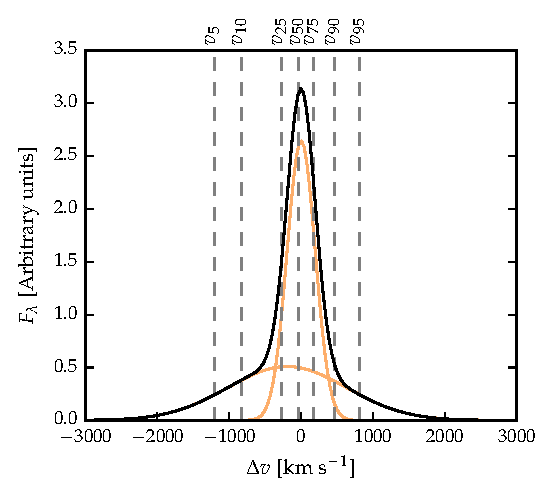
\includegraphics[width=0.8\textwidth]{figures/chapter04/example_oiii.pdf} 
    \caption[{}]{Non-parametric measures of the [\ion{O}{III}] velocity-profile, as described in the text.}     
    \label{fig:example_oiii}
\end{figure}

All [\ion{O}{III}] line properties are derived from the [\ion{O}{III}]\l$5008$ peak, but, as described above, the kinematics of [\ion{O}{III}]\l$4960$ are constrained to be identical in our fitting routine. 

We do not attach any physical meaning to the individual Gaussian components used in the model. 
Decomposing the [\ion{O}{III}] emission into a narrow component at the systemic redshift and a lower-amplitude, blueshifted broad component is often highly degenerate and dependent on the spectral S/N and resolution. 
Furthermore, there is no theoretical justification that the broad component should have a Gaussian profile.  

We therefore choose to characterize the [\ion{O}{III}] line profile using a number of non-parametric measures, which are commonly used in the literature \citep[e.g.][]{whittle85,zakamska14,zakamska16}. 
A normalised cumulative velocity distribution is constructed from the best-fitting model, from which the velocities below which $5$, $10$, $25$, $50$, $75$, $90$, and $95$ per cent of the total flux accumulates can be calculated. 
These velocities are then adjusted so that the peak of the [\ion{O}{III}] emission is at $0$\,\kms. 
The [\ion{O}{III}] velocities for an example model are shown in Figure~\ref{fig:example_oiii} 

We calculate the velocity-width containing $90$ per cent of the flux $w_{90}$ by rejecting $5$ per cent of the flux in the blue and red wings of the profile ($w_{90}\equiv v_{95} - v_{5}$).
We also calculate $w_{80}$ ($\equiv v_{90} - v_{10}$) and $w_{50}$ ($\equiv v_{75} - v_{25}$).
$w_{90}$ is relatively most sensitive to the flux in the wings of the line, whereas $w_{50}$ is relatively most sensitive to the flux in the core.  
In terms of the FWHM, $w_{50} \simeq {\mathrm FWHM} / 1.746$, $w_{80} \simeq {\mathrm FWHM} / 0.919$, $w_{90} \simeq {\mathrm FWHM} / 0.716$, assuming a Gaussian line profile.  

% remove page number from this page only
\afterpage{%
\thispagestyle{empty}
\begin{table}
  \centering
  \footnotesize
  \caption{The format of the table containing the emission-line properties from our parametric model fits. \todoinline{Available online.}}
  \label{tab:nlr-specmeasure}
  \centering
    \begin{tabular}{cccc} 
    \hline
    Column & Name & Units & Description \\ 
    \hline
    1 & UID & & Catalogue name \\
    2 & OIII\_V$5$ & \kms & [\ion{O}{III}] $v_{5}$ \\
    3 & OIII\_V$5$\_ERR & \kms & \\
    4 & OIII\_V$10$ & \kms & [\ion{O}{III}] $v_{10}$ \\
    5 & OIII\_V$10$\_ERR & \kms &  \\
    6 & OIII\_V$25$ & \kms & [\ion{O}{III}] $v_{25}$ \\
    7 & OIII\_V$25$\_ERR & \kms &  \\
    8 & OIII\_V$50$ & \kms & [\ion{O}{III}] $v_{50}$ \\
    9 & OIII\_V$50$\_ERR & \kms &  \\
    10 & OIII\_V$75$ & \kms & [\ion{O}{III}] $v_{75}$ \\
    11 & OIII\_V$75$\_ERR & \kms &  \\
    12 & OIII\_V$90$ & \kms & [\ion{O}{III}] $v_{90}$ \\
    13 & OIII\_V$90$\_ERR & \kms &  \\
    14 & OIII\_V$95$ & \kms & [\ion{O}{III}] $v_{95}$ \\
    15 & OIII\_V$95$\_ERR & \kms &  \\
    16 & OIII\_Z & & [\ion{O}{III}] redshift \\
    17 & OIII\_Z\_ERR & &  \\
    18 & OIII\_W$50$ & \kms & [\ion{O}{III}] $w_{50}$ \\
    19 & OIII\_W$50$\_ERR & \kms &  \\
    20 & OIII\_W$80$ & \kms & [\ion{O}{III}] $w_{80}$ \\
    21 & OIII\_W$80$\_ERR & \kms & \\
    22 & OIII\_W$90$ & \kms & [\ion{O}{III}] $w_{90}$ \\
    23 & OIII\_W$90$\_ERR & \kms & \\
    24 & OIII\_A & & [\ion{O}{III}] asymmetry \\
    25 & OIII\_A\_ERR & & \\
    26 & OIII\_EQW & \AA & [\ion{O}{III}] EQW \\
    27 & OIII\_EQW\_ERR & \AA & \\
    28 & OIII\_LUM & \ergs & [\ion{O}{III}] luminosity \\
    29 & OIII\_LUM\_ERR & \ergs & \\
    30 & EQW\_FE\_$4434$\_$4684$ & \AA & \ion{Fe}{II} EQW \\
    31 & EQW\_FE\_$4434$\_$4684$\_ERR & \AA & \\
    32 & HB\_VPEAK & \kms & \hb peak velocity \\
    33 & HB\_VPEAK\_ERR & \kms & \\
    34 & HA\_VPEAK & \kms & \ha peak velocity \\
    35 & HA\_VPEAK\_ERR & \kms & \\
    36 & HB\_Z & & \hb redshift \\
    37 & HB\_Z\_ERR & & \\
    38 & HA\_Z & & \ha redshift \\
    39 & HA\_Z\_ERR & & \\
    40 & OIII\_FE\_FLAG & & Bad \ion{Fe}{II} subtraction \\
    41 & OIII\_EXTREM\_FLAG & & Extreme [\ion{O}{III}] emission \\
    42 & BLUESHIFT\_CIV\_OIII & \kms & \ion{C}{IV} blueshift, relative to [\ion{O}{III}] \\
    43 & BLUESHIFT\_CIV\_OIII\_ERR & \kms &  \\
    \hline
    \end{tabular}
\end{table}
\clearpage
}

All of the derived parameters we have calculated are summarised in Table~\ref{tab:nlr-specmeasure}. The columns are as follows: 

\begin{itemize}
    
  \item[1] Catalogue name. 

  \item[2-15] $v_{5}$, $v_{10}$, $v_{25}$, $v_{50}$, $v_{75}$, $v_{90}$ and $v_{95}$ velocity of [\ion{O}{III}], relative to [\ion{O}{III}] peak, $v_{\mathrm peak}$, and their errors, in \kms.  

  \item[16-17] Systemic redshift measured at [\ion{O}{III}] peak wavelength, and its error. 

  \item[18-23] $w_{50}$ ($\equiv v_{75} - v_{25}$), $w_{80}$ ($\equiv v_{90} - v_{10}$) and $w_{90}$ ($\equiv v_{95} - v_{5}$) velocity-width of [\ion{O}{III}], and their errors, in \kms.

  \item[24-25] Dimensionless [\ion{O}{III}] asymmetry $A$, and its error. The asymmetry is define as 

  \begingroup\makeatletter\def\f@size{11}\check@mathfonts
   \begin{eqnarray}
    A = \frac{(v_{90} - v_{\mathrm peak}) - (v_{\mathrm peak} - v_{10})}{(v_{90} - v_{10})} \nonumber.     
    \end{eqnarray}  
  \endgroup

  \item[26-27] Rest-frame [\ion{O}{III}] EQW, and its error, in \AA.

  \item[28-29] [\ion{O}{III}] luminosity, and its error, in \ergs. 

  \item[30-31] $4434$-$4684$\,\AA\, rest-frame \ion{Fe}{II} EQW, and its error, in \AA.  

  \item[32-33] Velocity of \hb peak, relative to [\ion{O}{III}] peak, and its error, in \kms. 

  \item[34-35] Velocity of \ha peak, relative to [\ion{O}{III}] peak, and its error, in \kms. 

  \item[36-37] Redshift of \hb peak, and its error.

  \item[38-39] Redshift of \ha peak, and its error.

  \item[40] \ion{Fe}{II} flag. When flag is $1$ \ion{Fe}{II}-subtraction procedure has been unsuccessful (Section~\ref{sec:ch4-fe-removal}).  

  \item[41] Extreme [\ion{O}{III}] flag. When flag is $1$ [\ion{O}{III}] emission is extremely broad and blueshifted (Section~\ref{sec:extreme_oiii}). 

  \item[42-43] \ion{C}{IV} $v_{50}$, relative to [\ion{O}{III}] peak, and its error, in \kms.

\end{itemize}

\subsection{Deriving uncertainties on parameters}

To estimate realistic uncertainties on emission-line parameters derived from the best-fitting model we use the same Monte Carlo approach described in Section~\ref{sec:ch3_param_errors}. 
Very briefly, random simulations of each spectrum are generated.
Our fitting-procedure is run on each simulated spectrum, and the errors on the line parameters are estimated by measuring the spread of the parameter distribution from the ensemble of simulations. 
In a slight modification of the procedure in Section~\ref{sec:ch3_param_errors}, the error is defined as half the $68$ ($84$ - $16$) percentile spread in the parameter values. 

\subsection{Flagging low EQW [\ion{O}{III}]}
\label{sec:ch4-loweqw}

\begin{figure}
    \centering
    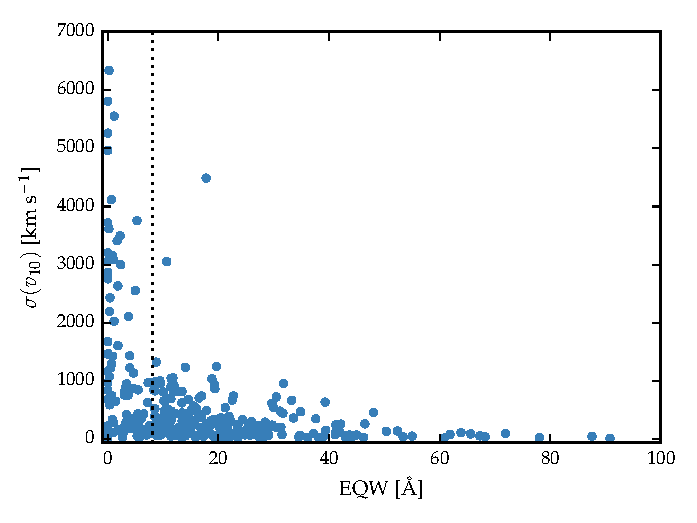
\includegraphics[width=0.8\textwidth]{figures/chapter04/eqw_cut.pdf} 
    \caption[{Uncertainty in $v_{10}$ as a function of the EQW, for [\ion{O}{III}].}]{Uncertainty in $v_{10}$ as a function of the EQW, for [\ion{O}{III}]. Uncertainties in $v_{10}$ are large to the left of the vertical line, at $8$\,\AA. These objects are ignored in our subsequent analysis of the [\ion{O}{III}] line shape.}     
    \label{fig:eqw_cut}
\end{figure}

In Figure~\ref{fig:eqw_cut} we show how the uncertainty in [\ion{O}{III}] $v_{10}$ depends on the EQW. 
As the strength of [\ion{O}{III}] decreases, the average uncertainty in $v_{10}$ increases.
When the [\ion{O}{III}] ${\mathrm EQW} > 80$\,\AA, the mean uncertainty in $v_{10}$ is $50$\,\kms; this increases to $450$\,\kms\, when $10 < {\mathrm EQW} < 20$\,\AA. 
As the EQW drops below $8$\,\AA, uncertainties in $v_{10}$ become very large (exceeding $1000$\,\kms\, in many objects). 
Clearly, the emission-line is too weak for its shape to be reliably measured in many of these objects. 
Therefore, when the [\ion{O}{III}] line properties (e.g. velocity-width, centroid) are analysed in later sections, objects with ${\mathrm EQW} < 8$\,\AA\, will be excluded. 
This leaves $226$ quasars in the sample. 

\subsection{Reliability of systemic redshift estimates}
\label{sec:ch4_redshifts}

\begin{figure}
   \captionsetup[subfigure]{labelformat=empty}
    \centering
    \subfloat[\label{fig:redshift_comparison_a}]{}
    \subfloat[\label{fig:redshift_comparison_b}]{}
    \subfloat[\label{fig:redshift_comparison_c}]{}
    \subfloat[]{{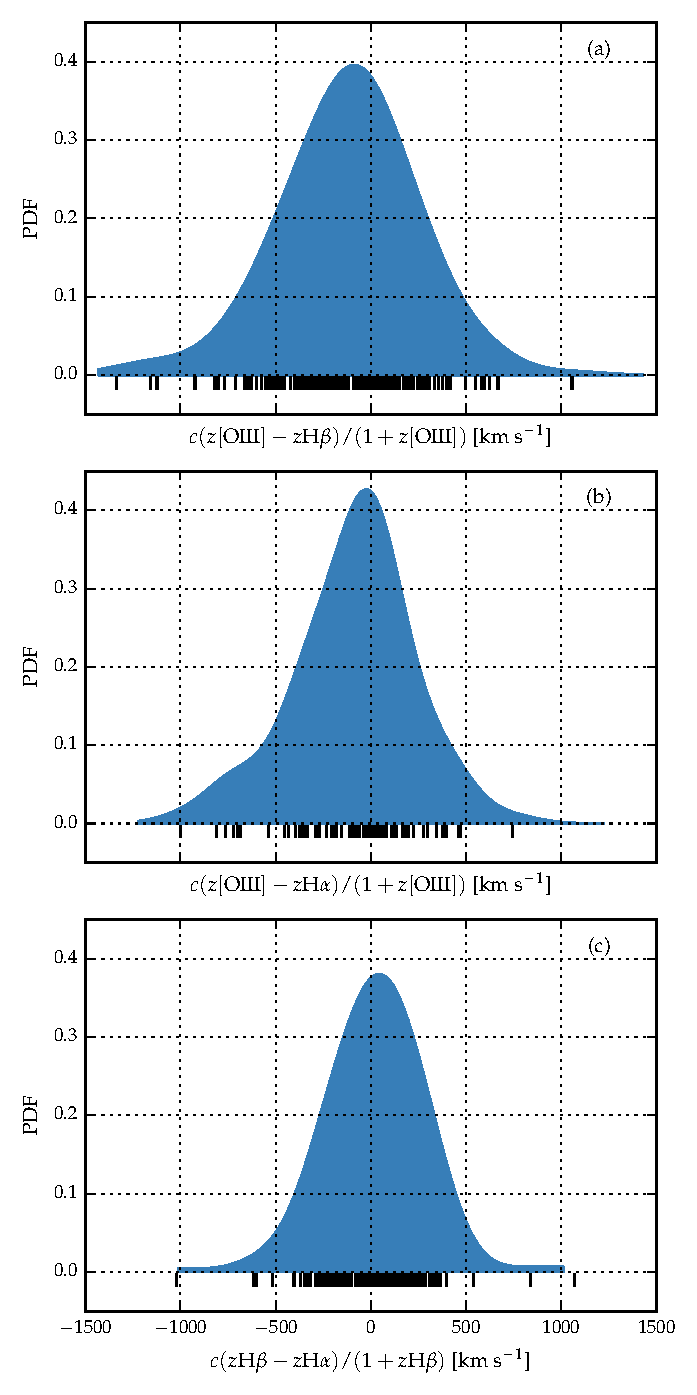
\includegraphics[width=0.8\linewidth]{figures/chapter04/redshift_comparison.pdf} }}
    \caption[{Comparison of systemic redshift estimates using [\ion{O}{III}], \hb and \hans.}]{Comparison of systemic redshift estimates using [\ion{O}{III}], \hb and \hans. The probability density distributions are generated using a Gaussian kernel density estimator with $170$, $120$ and $140$\,\kms\, kernel widths for (a), (b) and (c) respectively. The short black lines show the locations of the individual points.}       
    \label{fig:redshift_comparison}
\end{figure}

In this section, we compare systemic redshift estimates based on [\ion{O}{III}], \hb and \hans. 
The wavelength of each of these lines is measured at the peak of the emission and this measurement is made using the best-fitting parametric model. 
In the case of the Balmer lines, this model includes both broad and (if present) narrow emission features. 

We compare systemic redshift estimates based on [\ion{O}{III}] and \hb (Figure~\ref{fig:redshift_comparison_a}), [\ion{O}{III}] and \ha (Figure~\ref{fig:redshift_comparison_b}) and \hb and \ha (Figure~\ref{fig:redshift_comparison_c}). 
We generate probability density distributions using a Gaussian kernel density estimator.
The bandwidth, which is optimised using leave-one-out cross-validation, is $170$, $120$ and $140$\,\kms\, for samples (a), (b) and (c) respectively. 

There are $182$, $85$ and $162$ objects being compared in samples (a), (b) and (c) respectively. 
We have excluded [\ion{O}{III}], \hb and \ha measurements when the uncertainties on the peak velocities exceed $200$, $300$ and $200$\,\kms\, respectively. 
We also exclude [\ion{O}{III}] measurements from 16 objects with very broad, blueshifted [\ion{O}{III}] emission that is strongly blended with the red wing of \hb (these objects are discussed in Section~\ref{sec:extreme_oiii}).

The scatter between the different redshift estimates ($360$, $280$, and $230$\,\kms\, for (a), (b) and (c) respectively) is consistent with previous studies of redshift uncertainties from broad emission-lines \citep[e.g.][]{shen16b}. 
The systematic offset between the \ha and \hb estimates is effectively zero. 
However, the [\ion{O}{III}] redshifts appear to be systematically offset in comparison to both \ha and \hbns, in the sense that [\ion{O}{III}] is blueshifted in the rest-frame of the Balmer lines. 
This effect is strongest when [\ion{O}{III}] is compared to \hbns, in which case [\ion{O}{III}] is shifted by $\sim100$\,\kms\, to the blue.

\citet{hewett10} found that [\ion{O}{III}] was blueshifted by $\sim45$\,\kms\, relative to a rest-frame defined using photospheric \ion{Ca}{II}\ll$3935$,$3970$ absorption in the host galaxies of $z<0.4$ SDSS AGN and that [\ion{O}{III}] is increasingly blue-asymmetric at higher luminosities. 
Therefore, the $100$\,\kms offset we measure is consistent with \citet{hewett10} once the very different luminosities of the two samples are accounted for. 

\section{Results}

\subsection{Strength and kinematics of [\ion{O}{III}]}
\label{sec:ch4-basicresults}

\begin{figure}
    \captionsetup[subfigure]{labelformat=empty}
    \centering
    \subfloat[\label{fig:parameter_hists_a}]{}
    \subfloat[\label{fig:parameter_hists_b}]{}
    \subfloat[\label{fig:parameter_hists_c}]{}
    \subfloat[]{{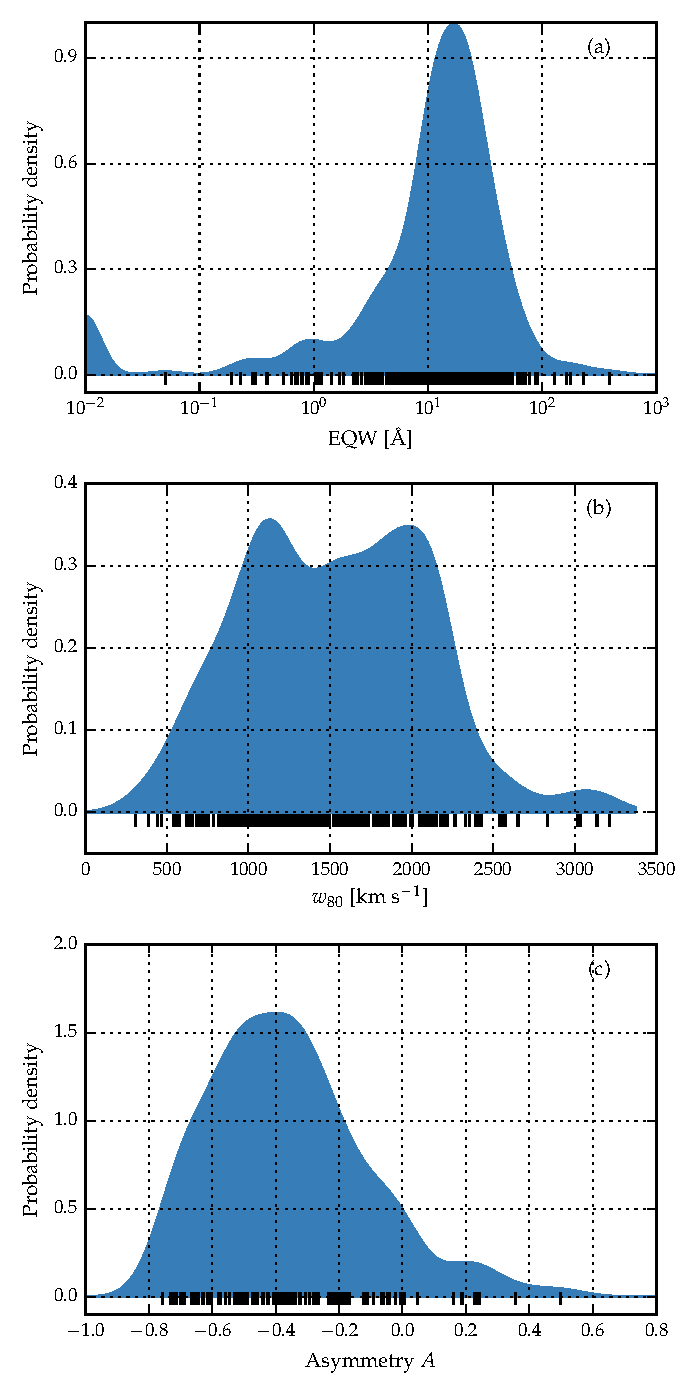
\includegraphics[width=0.8\columnwidth]{figures/chapter04/parameter_hists.pdf} }}
    \caption[{Probability density distributions of the [\ion{O}{III}] parameters EQW (a), $w_{80}$ (b) and asymmetry $A$ (c).}]{Probability density distributions of the [\ion{O}{III}] parameters EQW (a), $w_{80}$ (b) and asymmetry $A$ (c), generated using Gaussian kernel density estimator. The $1200$\,\kms\, upper limit on the velocity-width of the Gaussian functions used to model [\ion{O}{III}] is responsible for the peak at $1200$\,\kms\, in (b).}     
    \label{fig:parameter_hists}
\end{figure}

In our sample of $354$ quasars we observe a significant diversity in [\ion{O}{III}] emission properties. 

The probability density distribution of the [\ion{O}{III}] EQW is shown in Figure~\ref{fig:parameter_hists_a}. 
The median of the distribution is $14$\,\AA\, and the $68$ percentile range is $3$ to $30$\,\AA.
The maximum EQW is $391$\,\AA.  
In $10$ per cent of the sample [\ion{O}{III}] is very weak, with ${\mathrm EQW} < 1$\,\AA.  

The median of the line-width (characterized by $w_{80}$ and shown in Figure~\ref{fig:parameter_hists_b}) is $1540$\,\kms\, and the $68$ percentile range is $950$ to $2100$\,\kms, with a minimum of $300$\,\kms\, and a maximum of $3200$\,\kms.

The [\ion{O}{III}] asymmetry is shown in Figure~\ref{fig:parameter_hists_c}. 
In $40$ per cent of the sample [\ion{O}{III}] is fit with a single Gaussian. 
The asymmetry is zero in this model and so these objects are excluded. 
For the [\ion{O}{III}] emission-lines modelled with two Gaussians, [\ion{O}{III}] is blue-asymmetric in $90$ per cent.
The median asymmetry is $-0.37$ and the $68$ percentile range is $-0.61$ to $-0.12$.

Blue-asymmetric structure and high-velocity gas is generally associated with outflows. 
Our results suggests that NLR outflows are prevalent in this sample of luminous quasars. 

We also find weak correlations between these three [\ion{O}{III}] parameters. 
The EQW is anti-correlated with both the line-width and asymmetry: as the [\ion{O}{III}] emission gets weaker it gets broader and more blue-asymmetric \citep[e.g.][]{shen14}.  

\subsection{Luminosity-dependence of [\ion{O}{III}] properties}

In this section, we compare our sample of luminous $2 \lesssim z \lesssim 4$ quasars to a sample of $z\lesssim1$ SDSS quasars in order to investigate the luminosity and redshift dependence of key [\ion{O}{III}] parameters. 
We use $20\,663$ quasars with [\ion{O}{III}] measurements from the \citet{shen11} catalogue. 
The median redshift of these objects is $0.55$ and the median bolometric luminosity is $10^{45.5}$\,\ergs.

\begin{figure}[t!]
\centering 
    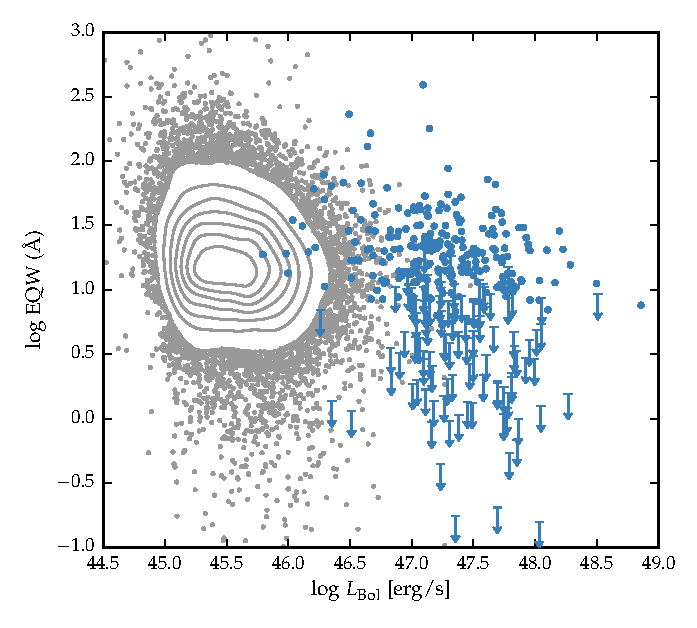
\includegraphics[width=\columnwidth]{figures/chapter04/eqw_lum.pdf} 
    \caption[{The [\ion{O}{III}] EQW as a function of the quasar bolometric luminosity for the sample presented in this chapter (blue circles) and the low-$z$ SDSS sample (grey points and contours).}]{The [\ion{O}{III}] EQW as a function of the quasar bolometric luminosity for the sample of luminous quasars presented in this chapter and the $z\lesssim1$ SDSS sample. An upper limit at ${\mathrm EQW}=1$\,\AA\, indicates points with ${\mathrm EQW} < 1$\,\AA. The red line shows the median [\ion{O}{III}] EQW in luminosity as a function of luminosity. The average EQW decreases from $18$ to $12$\,\AA\, over the luminosity range considered. At the same time, the fraction of quasars with very weak [\ion{O}{III}] (${\mathrm EQW} < 1$\,\AA) is ten times higher in the luminous quasar sample.}     
    \label{fig:eqw_lum}
\end{figure}

In Figure~\ref{fig:eqw_lum} we show the [\ion{O}{III}] EQW as a function of the quasar bolometric luminosity. 
Bolometric luminosities are estimated from monochromatic continuum luminosities at $5100$\,\AA, using the correction factor given by \citet{richards06}. 
Considering only the objects for which [\ion{O}{III}] is detected with ${\mathrm EQW} > 1$\,\AA, we observe a modest decrease in the [\ion{O}{III}] EQW as the luminosity increases (from $18$\,\AA\, at $L_{\mathrm Bol}=10^{45.25}$\,\ergs\, to $12$\,\AA\, at $L_{\mathrm Bol}=10^{47.75}$\,\ergs). 
However, [\ion{O}{III}] ${\mathrm EQW} < 1$\,\AA\, in $10$ per cent of the luminous quasars, compared to just one per cent of the $z \lesssim 1$ SDSS sample.
This is explored further in Section~\ref{sec:ch4-civtrends}.  

Many authors have reported the [\ion{O}{III}] EQW to decrease with quasar luminosity \citep[e.g.][]{brotherton96,sulentic04,baskin05b,zhang11,stern12}.
The origin of this correlation - known as the [\ion{O}{III}] Baldwin effect \citep[e.g.][]{baldwin77} - has not been demonstrated conclusively. 
The size of the NLR (and hence the [\ion{O}{III}] luminosity) is predicted to scale with the square root of the luminosity of the source of ionising photons \citep[e.g.][]{netzer90} and low-luminosity Seyfert galaxies appear to obey this relationship \citep[e.g.][]{bennert02}. 
Extrapolating this relationship to high luminosity quasars leads to the prediction of NLRs with galactic dimensions.
Under these conditions, the size of the NLR will be limited by the density and ionisation state in the NLR. 
In other words, the NLR can't continue to grow beyond the radius at which there is no longer gas available to be ionised and the luminosity of the NLR will saturate \citep[e.g.][]{hainline13,hainline14}. 

\begin{figure}[t!]
    \centering
    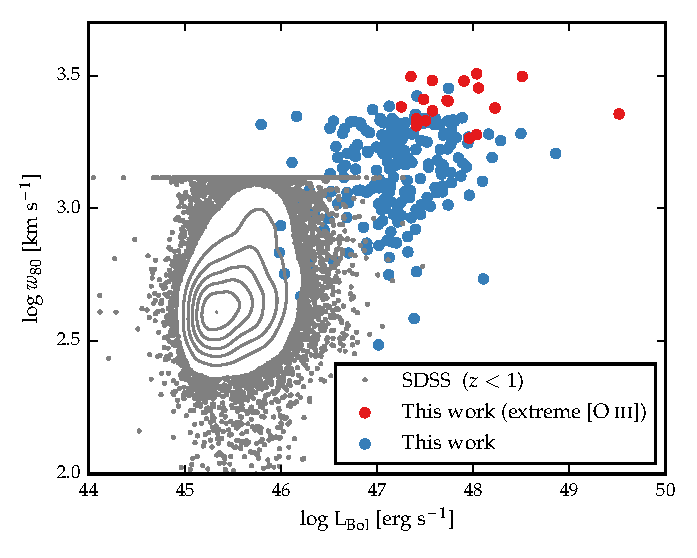
\includegraphics[width=\columnwidth]{figures/chapter04/lum_w80.pdf} 
    \caption[{}]{[\ion{O}{III}] velocity-width $w_{80}$ as a function of quasar bolometric luminosity. Objects with extreme [\ion{O}{III}] profiles (Section~\ref{sec:extreme_oiii}) are shown in red. The grey dots show $z\lesssim1$ SDSS quasars. The FWHM measurements given by \citet{shen11} have been converted into equivalent $w_{80}$ values by assuming $w_{80} \simeq {\mathrm FWHM} / 0.919$. The build-up of points at $w_{80}=1300$\,\kms\, is caused by the upper-limit $1200$\,\kms\, imposed by \citet{shen11} on the [\ion{O}{III}] FWHM. The typical [\ion{O}{III}] velocity-width increases from $440$\,\kms\, at $\log L_{\mathrm Bol}=45.5$\,\ergs\, to $1850$\,\kms\, at $\log L_{\mathrm Bol}=48$\,\ergs. \todoinline{Need to check 1+z in luminosity calculation.}} 
    \label{fig:lum_w80}
\end{figure}

In Figure~\ref{fig:lum_w80} we show that the [\ion{O}{III}] velocity-width is also strongly correlated with the quasar bolometric luminosity.
The typical [\ion{O}{III}] velocity-width increases from $440$\,\kms\, at $\log L_{\mathrm Bol}=45.5$\,\ergs\, to $1850$\,\kms\, at $\log L_{\mathrm Bol}=48$\,\ergs.  
This demonstrates that the highest velocity outflows are associated with the most luminous AGN which suggests that the outflows are driven by radiative forces. 

Considering only objects in a narrow luminosity range ($47 < \log L_{\mathrm Bol} < 47.5$\,\ergs) we observe no correlations between the redshift and either the [\ion{O}{III}] velocity-width or EQW.   
The lack of any evolution in typical [\ion{O}{III}] properties between $z=0$ and $z=1.5$ has previously been reported \citep[e.g.][]{harrison16}; our sample demonstrates that the [\ion{O}{III}] properties do not evolve from $z=1.5$ all the way to $z=4$. 

\subsection{EV$1$ trends in high-redshift quasars}

\begin{figure}[t!]
\centering 
    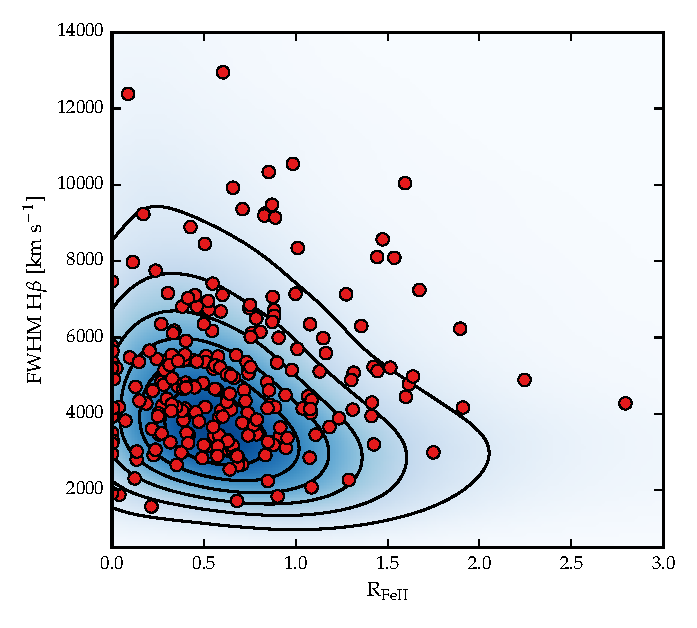
\includegraphics[width=\columnwidth]{figures/chapter04/ev1_lowz.pdf} 
    \caption[{EV$1$ parameter space.}]{The distribution of objects in the EV$1$ parameter space. The distribution of luminous quasars (shown using circles) is similar to the distribution of $z \lesssim 1$ SDSS quasars (shown using contours), with the displacement to higher \hb FWHM indicative of higher BH masses in the luminous sample.}      
    \label{fig:ev1_lowz}
\end{figure}

The FWHM of the broad \hb emission-line, the strength of [\ion{O}{III}] and the relative strengths of optical \ion{Fe}{II} and \hb have been identified as the features responsible for the largest variance in the spectra of AGN and form part of EV$1$ \citep{boroson92}.   
In Figure~\ref{fig:ev1_lowz} we show the [\ion{O}{III}] EQW as a function of the \hb FWHM and the optical \ion{Fe}{II} strength. 
The optical \ion{Fe}{II} strength is defined as the ratio of the \ion{Fe}{II} and \hb EQW, where the \ion{Fe}{II} EQW is measured between $4434$ and $4684$\,\AA.
There are $231$ objects in our sample with spectra that include \hbns, [\ion{O}{III}], and at least $150$\,\AA\, of the $4434$-$4684$\,\AA\, \ion{Fe}{II} region.  
For comparison, $z\lesssim1$ SDSS quasars are also shown in Figure~\ref{fig:ev1_lowz}. 
 
In our sample, the EV$1$ parameters follow similar correlations to what is observed at low-redshift.
In particular, we observe a strong anti-correlation between the [\ion{O}{III}] and \ion{Fe}{II} EQW.  
The \hb FWHM are displaced to higher values, which is consistent with the high-redshift, high-luminosity sample having larger BH masses. 
Thus, with a much bigger sample, we confirm earlier results suggesting that the same EV$1$ correlations exist in high-redshift quasars \citep[e.g.][]{netzer04,sulentic04,sulentic06,runnoe13,shen16a}.
This suggests that similar underlying physical processes govern the spectral properties of AGN and quasars over a wide range of redshifts and luminosities. 

\subsection{Connections with \ion{C}{IV} emission properties}
\label{sec:ch4-civtrends}

\begin{figure}[t!]
\centering 
    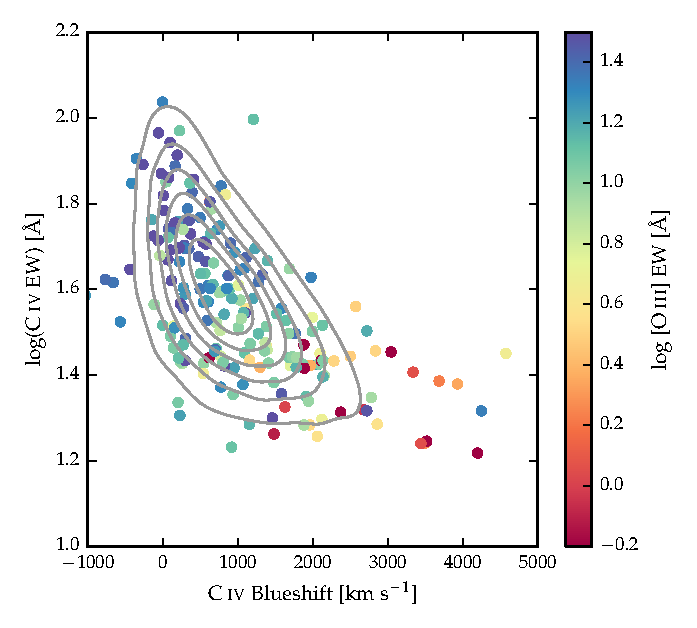
\includegraphics[width=0.9\textwidth]{figures/chapter04/ev1.pdf} 
    \caption[]{Parameter space of \ion{C}{IV} blueshift and EQW. Our sample is shown with the coloured circles, and quasars from the full SDSS catalogue are shown with grey contours. The [\ion{O}{III}] EQW varies systematically across the \ion{C}{IV} blueshift-EQW parameter space. In the small \ion{C}{IV} blueshift, high EQW region the mean [\ion{O}{III}] EQW is $47$\,\AA; this drops dramatically to $6$\AA\, in the large \ion{C}{IV} blueshift, low EQW region.}      
    \label{fig:ev1}
\end{figure}

Like the EV$1$ parameter space, the \ion{C}{IV} blueshift and EQW are diagnostics that similarly span the diversity of broad emission-line properties in high redshift quasars \citep{sulentic07,richards11}. 
In Figure~\ref{fig:ev1} we show the [\ion{O}{III}] EQW as a function of the \ion{C}{IV} blueshift and EQW.
When [\ion{O}{III}] is strong, the \ion{C}{IV} blueshift is measured relative to the [\ion{O}{III}] peak. 
Otherwise, the \ion{C}{IV} blueshift is measured relative to \hb or \hans.  
In Section~\ref{sec:ch4_redshifts} we found that redshifts measured from [\ion{O}{III}], \hb and \ha are consistent to within $\sim300$\,\kms, which is small in comparison to the dynamic range in \ion{C}{IV} blueshifts we see in Figure~\ref{fig:ev1}.
Also shown are the \ion{C}{IV} line parameters of $32\,157$ SDSS DR$7$ quasars at redshifts $1.6 < z < 3.0$. 
For this sample, systemic redshifts are taken from Allen \& Hewett (2017, in preparation). 

The [\ion{O}{III}] EQW decreases systematically from the small \ion{C}{IV} blueshift, large EQW region of the parameter space to the large \ion{C}{IV} blueshift, small EQW region.
In the top left of the distribution (\ion{C}{IV} blueshift $<1000$\,\kms, ${\mathrm EQW} > 60$\,\AA) the mean [\ion{O}{III}] EQW is $47$\,\AA; this drops dramatically to $6$\AA\, in the bottom right (\ion{C}{IV} blueshift $>2000$\,\kms, ${\mathrm EQW} < 30$\,\AA). 

Qualitatively, the distribution of objects in the \hb FWHM - \ion{Fe}{II} strength EV$1$ parameter space (Figure~\ref{fig:ev1_lowz}) is very similar to the distribution of objects in the \ion{C}{IV} blueshift-EQW parameter space (Figure~\ref{fig:ev1}).
In Figure~\ref{fig:line_comparison_ha} we showed that objects with large \ion{C}{IV} blueshifts also have narrow \ha emission-lines.
However, the converse is not true: many of the objects with narrow \ha emission-lines also have small \ion{C}{IV} blueshifts. 
In contrast, Figure~\ref{fig:ev1} demonstrates that the [\ion{O}{III}] EQW provides a less degenerate mapping between the EV$1$ and \ion{C}{IV} parameter spaces.

\begin{figure}
    \centering
    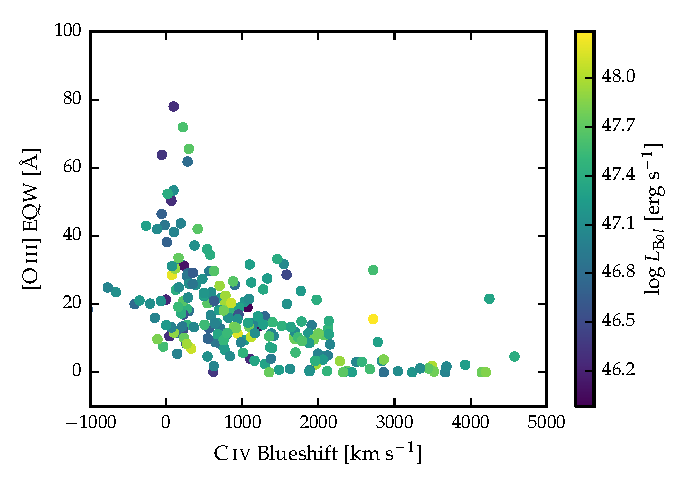
\includegraphics[width=\columnwidth]{figures/chapter04/civ_blueshift_oiii_eqw.pdf} 
    \caption[{[\ion{O}{III}] EQW as a function of the \ion{C}{IV} blueshift.}]{[\ion{O}{III}] EQW as a function of the \ion{C}{IV} blueshift. The [\ion{O}{III}] EQW is strongly anti-correlated with the \ion{C}{IV} blueshift. On the other hand, no strong luminosity-dependent trends (indicated by the colours of the points) are evident.}     
    \label{fig:civ_blueshift_oiii_eqw}
\end{figure}

A different projection of the same data is shown in Figure~\ref{fig:civ_blueshift_oiii_eqw}, which shows the [\ion{O}{III}] EQW as a function of the \ion{C}{IV} blueshift.  
The luminosity of the quasars is indicated by the colour of the points. 
Both the [\ion{O}{III}] EQW and the \ion{C}{IV} blueshift are known to depend on the quasar luminosity. 
However, Figure~\ref{fig:civ_blueshift_oiii_eqw} demonstrates that the strong correlation between the \ion{C}{IV} blueshift and [\ion{O}{III}] EQW is clearly not being driven by the mutual dependence of these parameters on the luminosity. 

Blueshifted \ion{C}{IV} emission is thought to arise in a high-velocity accretion disc wind.
The strong anti-correlation between the \ion{C}{IV} blueshift and the [\ion{O}{III}] EQW suggests that these outflows are having a dramatic impact on gas extended over kilo-parsec scales in the NLR.
Dynamical time-scales for the impact of fast moving outflows even on large NLRs are very short: it would take $10^6$ years for an outflow travelling at $3000$\,\kms\, to reach $3$\,kilo-parsec. 
Lifetimes of luminous quasars at these redshifts may be $10^7$ years \citep[e.g.][]{martini01}. 
Therefore, if the BLR outflows can break out in to the interstellar medium of the host-galaxy, the NLR can be cleared on a relatively short time-scale.
One possibility is that the BLR winds collide with the interstellar medium and shock and accelerate it to produce a galaxy-wide wind \citep[e.g.][]{king11,faucher12}. 
\ion{C}{IV} blueshifts are generally weaker in lower-luminosity quasars. 
Therefore, this picture also explains our finding that objects with very weak [\ion{O}{III}] (${\mathrm EQW} < 1$\,\AA) are ten times rarer in $z \lesssim 1$ SDSS quasars than in our sample of luminous quasars.   
\todo{Paul: does this sound right? Other explanations?}

\subsection{A link between BLR and NLR outflows}

\begin{figure}
\captionsetup[subfigure]{labelformat=empty}
\centering 
    \subfloat[\label{fig:oiii_civ_blueshifts_a}]{}
    \subfloat[\label{fig:oiii_civ_blueshifts_b}]{}
    \subfloat[\label{fig:oiii_civ_blueshifts_c}]{}
    \subfloat[]{{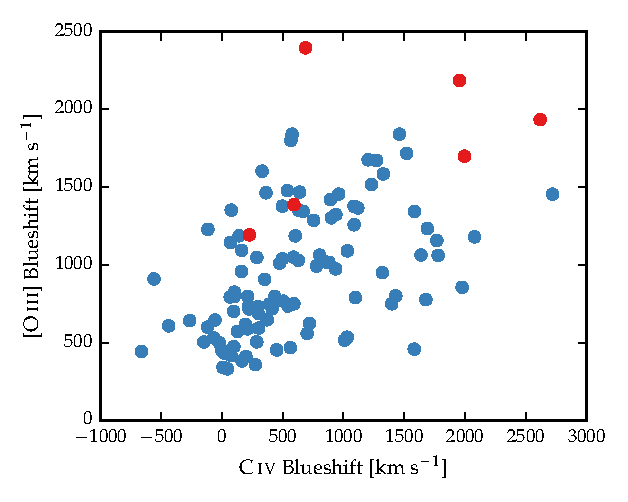
\includegraphics[width=\linewidth]{figures/chapter04/civ_blueshift_oiii_blueshift.pdf} }}
    \caption[{The relation between the blueshifts of \ion{C}{IV} and [\ion{O}{III}].}]{Relationship between the \ion{C}{IV} ($v_{50}$(\ion{C}{IV}) - $v_{\mathrm peak}$([\ion{O}{III}])) and [\ion{O}{III}] ($v_{10}$([\ion{O}{III}]) - $v_{\mathrm peak}$([\ion{O}{III}])) blueshift.  The \ion{C}{IV} and [\ion{O}{III}] blueshifts are correlated with $\rho_{\mathrm S}=0.46$. This correlation is independent of the luminosity (indicated by the colour of the points). Objects with errors on the [\ion{O}{III}] and \ion{C}{IV} blueshifts exceeding $250$ or $125$\,\kms\, respectively are not shown in (c); these objects fall above the dashed line in (a) and (b). }     
    \label{fig:oiii_civ_blueshifts}
\end{figure}


In Figure~\ref{fig:oiii_civ_blueshifts_c} we show that the [\ion{O}{III}] blueshift is correlated with the \ion{C}{IV} blueshift ($\rho_{\mathrm S}=0.46$, p-value $=6e\text{-}7$). 
This shows that high-velocity winds in the NLR are preferentially seen when strong winds are being driven in the vicinity of the central engine. 
As we demonstrate in Figure~\ref{fig:oiii_civ_blueshifts_c}, this correlation is not driven by the luminosity. 
Although we lack direct spatial information, this correlation suggests a connection between gas kinematics on sub-parsec and kilo-parsec scales. 

The [\ion{O}{III}] blueshift is defined as $v_{10}$([\ion{O}{III}]) - $v_{\mathrm peak}$([\ion{O}{III}]) and the \ion{C}{IV} blueshift is defined as $v_{50}$(\ion{C}{IV}) - $v_{\mathrm peak}$([\ion{O}{III}]).
We considered a number of alternative approaches to parametrising both the [\ion{O}{III}] line shape and the systemic redshift. 
Very similar trends are observed when the [\ion{O}{III}] line shape is parametrised using $v_{25} - v_{\mathrm peak}$, $v_{50} - v_{\mathrm peak}$, $w_{80} = v_{90} - v_{10}$, or the asymmetry $A$.
The same trend is also observed when the systemic redshift is defined using the peak of the \hb emission. 

In the previous section, we saw how [\ion{O}{III}] is very weak in quasars with \ion{C}{IV} blueshifts exceeding $\sim2000$\,\kms. 
The [\ion{O}{III}] blueshift cannot be reliably measured if the emission-line ${\mathrm EQW} \lesssim 8$ (Section~\ref{sec:ch4-loweqw}) and so this limits the dynamic range of \ion{C}{IV} blueshifts probed in Figure~\ref{fig:oiii_civ_blueshifts_c}. 
We do not show objects for which the errors on the [\ion{O}{III}] and \ion{C}{IV} blueshifts exceed $250$ or $125$\,\kms\, respectively. 
The [\ion{O}{III}] and \ion{C}{IV} blueshifts of these objects, shown in Figures~\ref{fig:oiii_civ_blueshifts_a} and \ref{fig:oiii_civ_blueshifts_b}, are similar to the main sample, meaning our results should not be biased by their exclusion.  
We also remove the objects with extreme [\ion{O}{III}] emission (Section~\ref{sec:extreme_oiii}), because the systemic redshift determined from the peak of the [\ion{O}{III}] emission is strongly biased in these objects. 

\citet{shen14} showed how the [\ion{O}{III}] EQW decreases as the optical \ion{Fe}{II} strength (which is related to the Eddington ratio) or luminosity increase. 
However, the amplitude of the systemic, core [\ion{O}{III}] emission decreases faster than the wing component.
A by-product of this effect is that the overall [\ion{O}{III}] profile becomes broader and more blueshifted, as the broad wing component becomes relatively more prominent.
If the anti-correlation between the [\ion{O}{III}] EQW and \ion{C}{IV} blueshift is primarily being driven by a reduction in the flux of the core component (as a stable NLR is removed by the outflowing material), this would lead to a correlation between the [\ion{O}{III}] blueshift and \ion{C}{IV} blueshift similar to the one seen in Figure~\ref{fig:oiii_civ_blueshifts_c}. 
This effect could also explain the anti-correlation between the [\ion{O}{III}] EQW and blue-asymmetry / velocity-width we reported in Section~\ref{sec:ch4-basicresults}. 

\subsection{Extreme [\ion{O}{III}] profiles}
\label{sec:extreme_oiii}

\begin{figure}
    \centering
    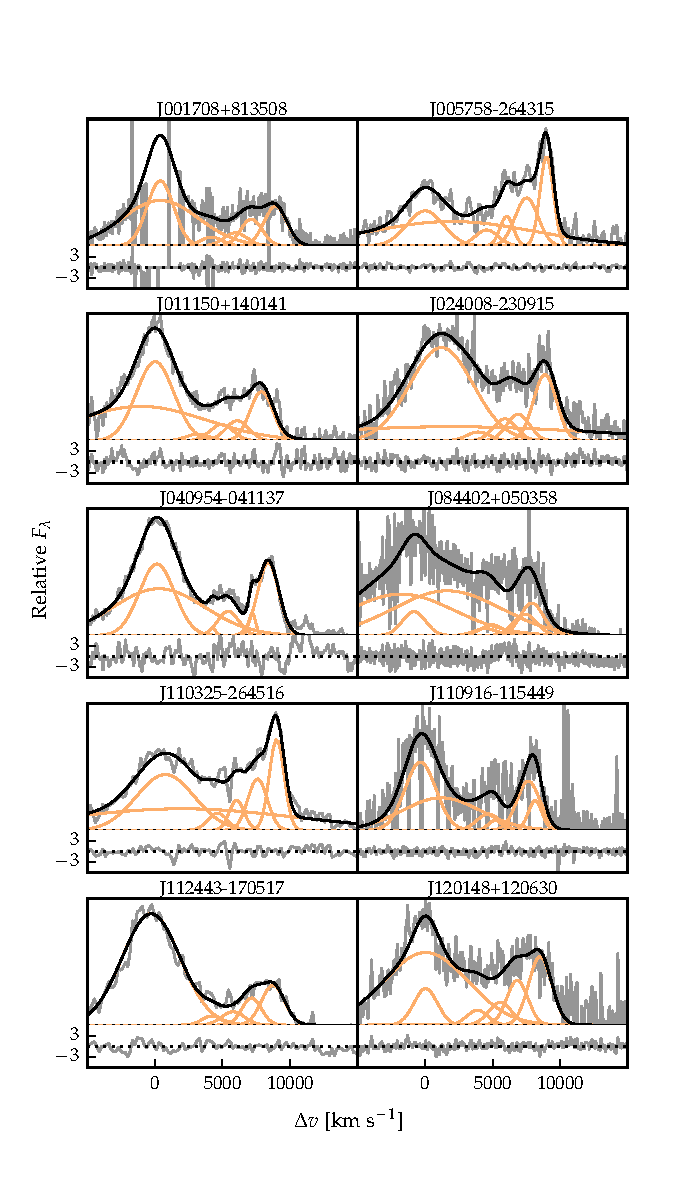
\includegraphics[width=\columnwidth]{figures/chapter04/example_spectrum_grid_extreme_oiii_1.pdf} 
    \caption[{Model fits to the continuum- and \ion{Fe}{II}-subtracted \hbns/[\ion{O}{III}] emission in $18$ quasars with extreme [\ion{O}{III}] emission profiles.}]{Model fits to the continuum- and \ion{Fe}{II}-subtracted \hbns/[\ion{O}{III}] emission in $18$ quasars with extreme [\ion{O}{III}] emission profiles. The data is shown in grey, the best-fitting model in black, and the individual model components in orange. The peak of the [\ion{O}{III}] emission is used to set the redshift, and $\Delta{v}$ is the velocity shift from the rest-frame transition wavelength of \hbns. Below each spectrum we plot the data- minus-model residuals, scaled by the errors on the fluxes.}     
    \label{fig:example_spectrum_grid_extreme_oiii}
\end{figure}

\begin{figure}
\ContinuedFloat
    \centering
    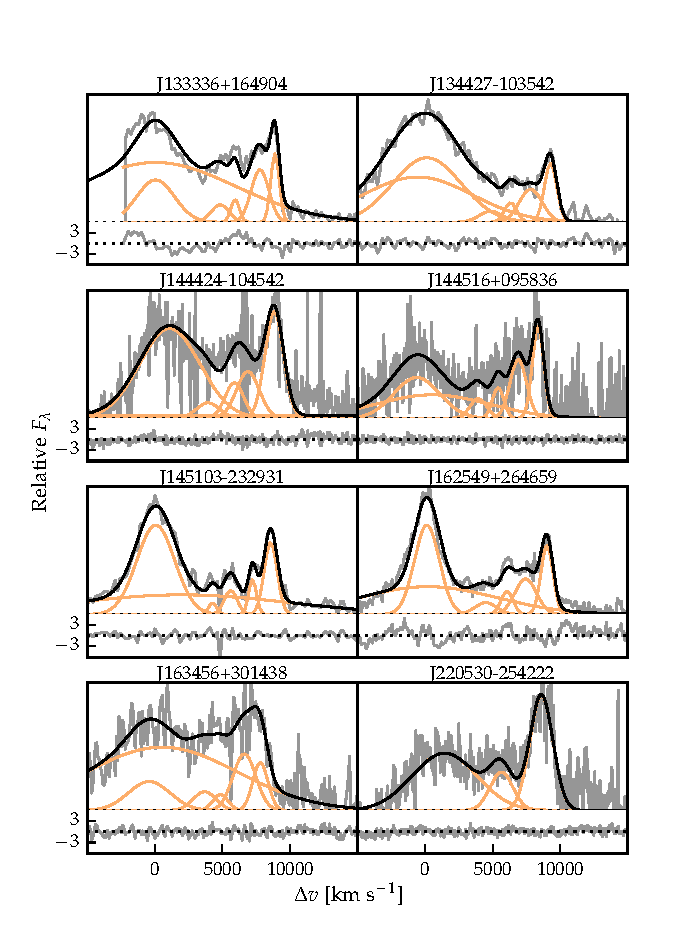
\includegraphics[width=\columnwidth]{figures/chapter04/example_spectrum_grid_extreme_oiii_2.pdf} 
    \caption[]{Continued.}     
\end{figure}

Figure~\ref{fig:example_spectrum_grid_extreme_oiii} shows the spectra of $18$ objects which we visually identified as having [\ion{O}{III}] emission profiles with similar characteristics to four extremely dust-reddened quasars at $z\sim2$ recently identified by \citet{zakamska16}. 
The extreme nature of the [\ion{O}{III}] emission in their sample of red quasars led \citet{zakamska16} to propose that these objects are being observed in the process of expelling the gas in their host-galaxies and transitioning from a dust-obscured, star-burst phase to a luminous, blue quasar \citep[e.g.][]{sanders88}.

The [\ion{O}{III}] emission in the $18$ objects in our sample is very broad ($1800 \lesssim w_{80} \lesssim 3200$\,\kms; Figure~\ref{fig:lum_w80}). 
In many of these objects the systemic, core component of [\ion{O}{III}] is not detected.
The [\ion{O}{III}] doublet is blended together, and is also heavily blended with the red wing of the \hb emission. 
The \ion{Fe}{II} emission may also be significant in this region of the spectrum. 

\begin{figure}
\centering 
    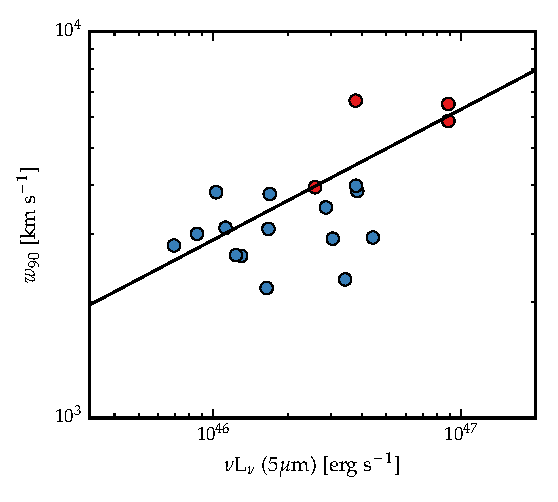
\includegraphics[width=0.8\textwidth]{figures/chapter04/fivemicron_w90.pdf} 
    \caption[{}]{Velocity-widths, $w_{90}$, and rest-frame $5$\,$\mu$m luminosities of the $18$ quasars in our sample with extreme [\ion{O}{III}] emission profiles and the four dust-reddened quasars from \citet{zakamska16}. Our sample falls on the width-luminosity relation derived by \citet{zakamska16}.}     
    \label{fig:fivemicron_w90}
\end{figure}

In Figure~\ref{fig:fivemicron_w90} we compare the velocity-widths and rest-frame $5$\,$\mu$m luminosities of the $18$ quasars in our sample with the four quasars from \citet{zakamska16}.
On average, the \citet{zakamska16} quasars have higher luminosities ($10^{46.7}$ versus $10^{46.3}$\ergs) and the [\ion{O}{III}] emission is broader ($5740$ versus $3120$\,\kms).
However, the [\ion{O}{III}] velocity-width and luminosity of the least extreme \citet{zakamska16} quasar has properties very similar to our sample, and our objects lie on top of the velocity-luminosity relation derived by \citet{zakamska16} (Figure~\ref{fig:fivemicron_w90}).

The [\ion{O}{III}] velocity-widths and luminosities of the $18$ quasars in Figure~\ref{fig:example_spectrum_grid_extreme_oiii} are very large, but are comparable to many other objects in our sample.
However, we find that of the six objects which fall within the footprint of the FIRST radio survey, four are radio-loud (three core-dominated and one lobe-dominated).
Given the fraction of radio-loud objects in our sample is $11$ per cent, the binomial probability of finding four radio-loud objects in a sample of six is $0.1$ per cent. 
Relativistic jets are known to accelerate gas to velocities of up to a few thousand \kms\, \citep[e.g.][]{nesvadba06,nesvadba08}, and this could be inducing the disturbed [\ion{O}{III}] gas kinematics of these objects. 

\section{Mass outflow rate and kinetic power}

The mass outflow rate and kinetic power of galaxy-wide outflows are important in order to understand the role played by quasars in the evolution of galaxies. 
In this section, we calculate the mass outflow rate ($\dot{M}$) and kinetic power ($P_{\mathrm K}$) of the ionised outflows in our sample of luminous quasars, using the [\ion{O}{III}] emission as a gas tracer \citep[e.g.][]{harrison12,cano-diaz12,liu13,brusa15,carniani15,bischetti16,kakkad16}.  
By making reasonable assumptions for unknown quantities (including the geometry, spatial scale and density of the gas in the outflow) we can calculate order of magnitude estimates of the outflow properties.
Our calculations are based on the model of \citet{cano-diaz12}, and a comprehensive description of the assumptions in the model and their impact on the inferred outflow properties can be found in \citet{cano-diaz12} and \citet{kakkad16}. 

Following \citet{cano-diaz12}, the mass in the ionised outflow is given by 

\begingroup\makeatletter\def\f@size{11}\check@mathfonts
\begin{eqnarray}
M \simeq 5.33 \times 10^7 \left( \frac{C}{10^{\mathrm[O/H] - [O/H]_\odot}} \right) \left( \frac{L([OIII])}{10^{44}\, {\mathrm erg}\,{\mathrm s}^{-1}}\right) \nonumber \\ \times \left\langle \frac{n_e}{10^3\, {\mathrm cm}^{-3}} \right\rangle^{-1} \, M_\odot
\end{eqnarray}
\endgroup

\noindent where $L([OIII])$ is the luminosity of [\ion{O}{III}] emitted in the outflow (in units of $10^{44}$\,\ergs), $\langle n_e \rangle$ is the electron density in the outflowing gas (in units of $10^3$\,cm$^{-3}$), $10^{[{\mathrm O/H}]}$ is the metallicity (in units of Solar metallicity), $C$ ($=\langle n_e \rangle ^2 / \langle n_e^2\rangle$) is the condensation factor (assumed to be $\simeq1$). 
Assuming a conical outflow with uniformly distributed clouds out to a radius $R$ with a constant outflow velocity, the mass outflow rate of the gas is given by: 

\begingroup\makeatletter\def\f@size{11}\check@mathfonts
\begin{eqnarray}
\dot{M} = 164 \left( \frac{R}{1\,{\mathrm kpc}} \right)^{-1} \left( \frac{C}{10^{\mathrm[O/H] - [O/H]_\odot}} \right) \left( \frac{L([OIII])}{10^{44}\, {\mathrm erg}\,{\mathrm s}^{-1}}\right) \nonumber \\ \times \left( \frac{v}{1000\,{\mathrm km}\,{\mathrm s}^{-1}}\right) \times \left\langle \frac{n_e}{10^3\, {\mathrm cm}^{-3}} \right\rangle^{-1} \, M_\odot \, {\mathrm yr^{-1}}
\end{eqnarray}
\endgroup

\noindent where $v$ is the outflow velocity (in units of $1000$\,\kms).
The kinetic power of the outflow ($1/2\dot{M}v^2$) is given by: 

\begingroup\makeatletter\def\f@size{11}\check@mathfonts
\begin{eqnarray}
P_{\mathrm K} = 5.17 \times 10^{43} \left( \frac{R}{1\,{\mathrm kpc}} \right)^{-1} \left( \frac{C}{10^{\mathrm[O/H] - [O/H]_\odot}} \right) \left( \frac{L([OIII])}{10^{44}\, {\mathrm erg}\,{\mathrm s}^{-1}}\right) \nonumber \\ \times \left( \frac{v}{1000\,{\mathrm km}\,{\mathrm s}^{-1}}\right)^3 \times \left\langle \frac{n_e}{10^3\, {\mathrm cm}^{-3}} \right\rangle^{-1} \, {\mathrm erg}\,{\mathrm s}^{-1}
\end{eqnarray}
\endgroup

\noindent We assume that the maximum outflow velocity ($\simeq v_{5}$) is representative of the average outflow velocity, with the lower velocities due to projection effects \citep{cano-diaz12}.
We assume the outflowing gas is represented by the broader of the two Gaussian components in our [\ion{O}{III}] model, and use the luminosity of this component to estimate the luminosity of the outflowing gas. 
This is not possible when [\ion{O}{III}] is modelled with a single Gaussian, and so these objects are not considered. 
For the outflow radius we use $4$\,kilo-parsec.
This is broadly consistent with spatially resolved observations of quasars at similar redshifts and luminosities \citep[e.g.][]{cano-diaz12,carniani15,brusa16} and photo-ionisation estimates \citep[e.g.][]{zakamska16}. 

With these values, we calculate outflow rates which range from a few to $4000\,M_\odot\,{\mathrm yr}^{-1}$. 
The mean for our sample is $560\,M_\odot\,{\mathrm yr}^{-1}$. 
In terms of the kinetic power of the outflows, this corresponds to values from about $10^{41.8}$ to $10^{45.7}$\,\ergs, with mean $10^{44.7}$\,\ergs. 
This kinetic power corresponds to $\sim0.15$ per cent of the bolometric luminosity, and this reaches almost $1$ per cent in the most powerful outflows.  
However, if the ionized outflow is accompanied by a neutral/molecular outflow an order of magnitude more massive then the kinetic power is also likely to be an order of magnitude higher \citep{cano-diaz12}, i.e. about $1.5$ per cent of the bolometric luminosity for the mean kinetic power and $10$ per cent for the most powerful outflows. 
These outflow efficiencies are in same ballpark as recent AGN feedback models \citep[e.g.][]{zubovas12}, which predict a coupling efficiency between AGN-driven outflows and AGN power of $\sim5$ per cent.
\todo{Double check luminosities!}

\section{Mean field independent component analysis}

Blind source separation (BSS) techniques can generate a set of component spectra that can then be combined with varying weights to reconstruct individual input spectra.
Principle component analysis (PCA) is one example of a BSS technique that has been applied extensively to analyse astronomical spectra \citep[e.g.][]{mittaz90,francis92,yip04}. 
However, while input spectra can be reconstructed from the PCA-derived components, in general it is not possible to physically interpret the individual components. 
Mean field independent component analysis (MFICA) is more powerful class of BSS technique that works by finding a basis of independent components to represent the data.  
\citet{allen13} used this technique to analyse the SDSS spectra of emission-line galaxies and demonstrated its effectiveness in identifying distinct emission sources in the spectra. 

In this chapter, we use a set of ten MFICA-derived spectral components to reconstruct the rest-frame optical spectra of luminous quasars.
The set of weights measured for each quasar provide a compact representation of its spectral properties.  
By equating components with physical properties of interest we can use the component weights in place of more commonly used emission-line parameters. 
We show below how the distribution of weights in the sample as a whole reveals many of the same results revealed in the first part of this chapter.  
At the same time, with the MFICA-derived components we are able to extend our analysis to a lower S/N regime than is possible with a more traditional approach (i.e. fitting multiple Gaussian components).

As we will show later in this section, initial results from the MFICA analysis are very promising.
Nevertheless, we face two outstanding issues.  
The first is the limited spectral diversity of the objects used to derive the components and the second is cross-talk between the independent components.
These are discussed below, together with our proposed solutions. 

\subsection{Generating the spectral components}

We use a set of ten spectral components that have been generated using MFICA from a carefully selected sample of $z \lesssim 1$ SDSS quasars\footnote{This was done by Prof. Paul Hewett.}.
The MFICA components were generated in the rest-frame interval $4000$-$5600$\,\AA.
This restricted the redshift range of the SDSS spectra that can be used to XX.  
A sample of $2,154$ SDSS quasars was selected.
Six positive independent components and four lower-amplitude `correction' components that can have negative weights were found to be sufficient to reconstruct the spectra. 
\todo{Ask Paul for details.} 

\subsection{Reconstructing input spectra}

\begin{figure}[t!]
    \centering
    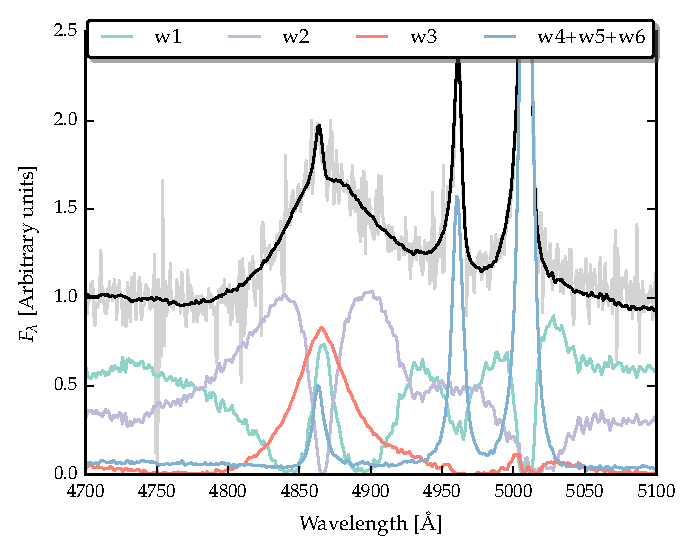
\includegraphics[width=0.8\textwidth]{figures/chapter04/mfica_components.pdf} 
    \caption{\hbns/[\ion{O}{III}] emission J$002952$+$020607$. The MFICA reconstruction is shown in black, and the spectrum in grey. The first three components, and the sum of components four, five and six are shown individually.}     
    \label{fig:mfica_components}
\end{figure}

Input spectra are reconstructed using a $\chi^2$ minimisation to determine the optimum set of component weights. 
Each of the individual MFICA components has been adjusted to give the same overall shape as a quasar template spectrum. 
We approximate the overall shape of this template by fitting a single power-law to emission-line free windows at $4200$-$4230$, $4435$-$4700$ and $5100$-$5535$\,\AA. 
We then flatten each of the MFICA components by dividing by this power-law. 
An identical process is performed on each spectrum we fit, so that both the components and the spectrum to be fitted have essentially zero large-scale slope. 
For each quasar in our sample we perform a variance-weighted least-squares minimisation to determine the optimum value of the components weights.
The first six component weights are constrained to be non-negative, and the fit is performed in logarithmic wavelength space, so that each pixel corresponds to a fixed velocity-width.   
The relative shift of the MFICA components is also allowed to vary in the optimisation procedure, to account for errors in the systemic redshifts used to transform the spectra into rest-frame wavelengths. 

In general, the components are able to accurately reproduce the spectra in our sample. 
We find the components are able to accurately reproduce the \ion{Fe}{II} emission in many of the objects for which the \citet{boroson92} template was a poor match. 
However, as discussed above, some of the broader [\ion{O}{III}] lines not well reproduced. 

As we showed in Section~XX, [\ion{O}{III}] emission properties are strongly luminosity dependent.
Specifically, [\ion{O}{III}] is broader, weaker and more asymmetric in more luminous quasars.  
There are insufficient numbers of objects in the $z<1$ SDSS sample with these characteristics. 
As a result, the MFICA-derived spectral components are unable to accurately reconstruct the very broad [\ion{O}{III}] emission-lines seen in luminous quasars. 
We can solve this by finding some more representative broad [\ion{O}{III}] lines in SDSS from which to derive the components. 


\subsection{Interpretation of individual components}

An example of this reconstruction is shown in Figure~\ref{fig:mfica_components}. 
The individual spectral components relate to the underlying physical constituents of the quasar. 
This correspondence is summarised in Table~\ref{tab:icacomps}. 
The component $w_1$ seems to correspond to \ion{Fe}{II} emission, the components $w_2$ and $w_3$ to broad \hb emission, the components $w_4$ and $w_5$ to narrow [\ion{O}{III}] emission at the systemic redshift, and the component $w_6$ to broad, blueshifted [\ion{O}{III}] emission. 

\begin{table}[t!]
  \centering
  \footnotesize 
  \caption{Physical interpretation of the ICA components.}
  \label{tab:icacomps}
    \begin{tabular}{cc} 
    \hline
    Component & Origin \\
    \hline
    $w_1$& \ion{Fe}{II} \\
    $w_2$& \hbns \\
    $w_3$& \hbns \\
    $w_4$& [\ion{O}{III}] core \\
    $w_5$& [\ion{O}{III}] core \\
    $w_6$& [\ion{O}{III}] wing \\
    \hline
    \end{tabular}
\end{table} 

\subsection{Reconstructing the [\ion{O}{III}] emission}

If the [\ion{O}{III}] emission is confined to a relatively small number of components can then recover emission. 
Discuss issue with cross talk. 
In the previous approach we measured non-parametric line parameters from the Gaussian model. 
We would like to be able to take a similar approach here. 
This requires us to first reconstruct the [\ion{O}{III}] emission. 
The vast majority of the [\ion{O}{III}] emission is in just three of the ICA components; the remaining three contribute very little. 
Therefore, we can set the first three weights to zero to leave only the [\ion{O}{III}] emission. 
However, there is some cross-talk between components, particularly in the wings of the line. 
This is something we can address in the future (ask Paul how). 

\subsection{Some results}

\begin{figure}
\centering 
    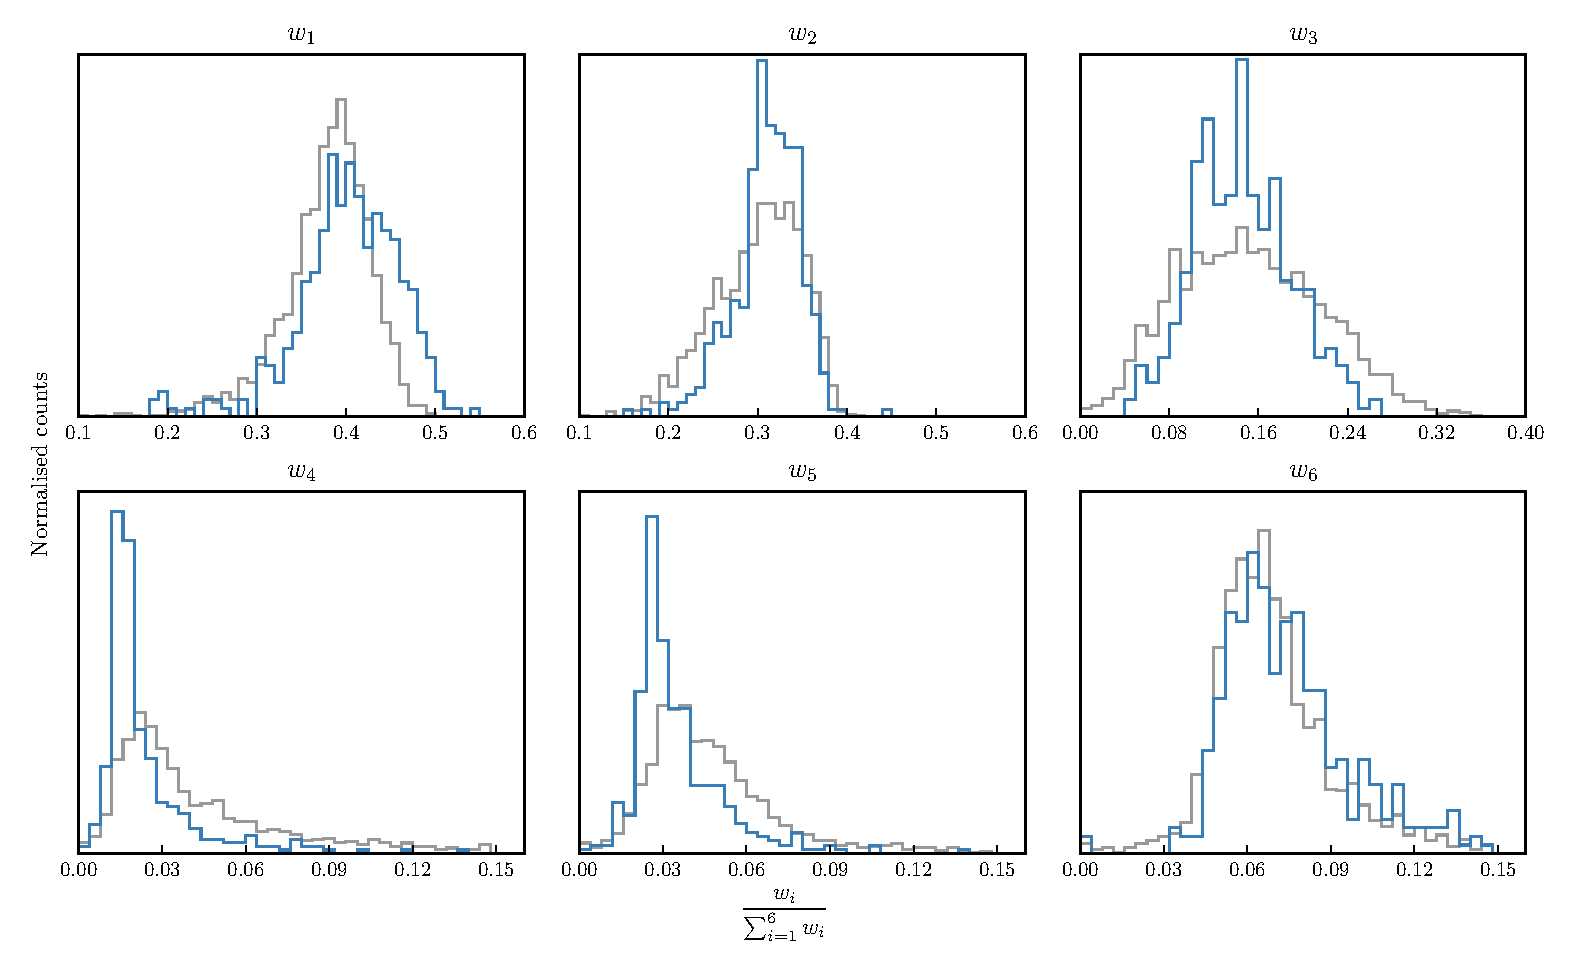
\includegraphics[width=\textwidth]{figures/chapter04/mfica_component_weights.pdf} 
    \caption[{The relative weight in each of the six positive ICA components for the high-luminosity and low luminosity samples.}]{The relative weight in each of the six positive ICA components for the high-luminosity (blue) and low luminosity samples (grey). In the high-luminosity sample \ion{Fe}{II} emission is stronger (component $w_1$). The core [\ion{O}{III}] emission (components $w_4$, $w_5$) is weaker but the strength of the blueshifted wing ($w_6$) is the same and so the relative contribution from the blueshifted component to the total [\ion{O}{III}] emission is higher.}     
    \label{fig:mfica_component_weights}
\end{figure}


In Figure~\ref{fig:mfica_component_weights} we show the relative weights of each of the six positive ICA components. 
Also shown are the same measurements for a sample of low-redshift, low-luminosity AGN. 

\begin{figure}
    \centering
    \includegraphics[width=\textwidth]{figures/chapter04/civ_blueshift_oiii_strength.pdf} 
    \caption[{The ICA component weight $w_4$, which is a proxy for the strength of core [\ion{O}{III}], as a function of the \ion{C}{IV} blueshift.}]{The ICA component weight $w_4$, which is a proxy for the strength of core [\ion{O}{III}], as a function of the \ion{C}{IV} blueshift. The \ion{C}{IV} blueshift is measured relative to the near-infrared ICA redshift.}     
    \label{fig:civ_blueshift_oiii_strength}
\end{figure}

\begin{figure}
    \centering
    \includegraphics[width=\columnwidth]{figures/chapter04/mfica_composites.pdf} 
    \caption[{Median ICA-reconstructed spectra as a function of the \ion{C}{IV} blueshift.}]{Median ICA-reconstructed spectra as a function of the \ion{C}{IV} blueshift.}     
    \label{fig:mfica_composites}
\end{figure}

There is a very well defined relation: when \ion{C}{IV} is strongly blueshifted [\ion{O}{III}] is very weak. 
This is very similar to what we found when we used Gaussian functions to model the emission. 
The correlation between \ion{C}{IV} blueshift and [\ion{O}{III}] EQW is shown in a different way in Figure~\ref{fig:mfica_composites}. 
Here we divide our sample into four bins according to the \ion{C}{IV} blueshift. 
From the quasars in each \ion{C}{IV} blueshift bin we then find then generate an ICA spectrum using the median weights from each quasar. 
The differences in the spectra as a function of the \ion{C}{IV} blueshift are dramatic. 
[\ion{O}{III}] becomes progressively weaker and more blueshifted.
The anti-correlation with \ion{Fe}{III} and the blue-ward \ion{Fe}{II} also clear, but there is no change in the redward \ion{Fe}{II}. 
ICA looks promising, and in the future, the weights could be added to EV$1$, or even replace the traditional components. 

We can take the median weights as a function of blueshift and use these to generation of high signal-to-noise ratio (S/N) examples of such spectra. 

\section{Summary}

\begin{itemize}

\item We have found that outflows in the NLR, as indicated by broad velocity-widths and asymmetries in [\ion{O}{III}], are ubiquitous in the luminous quasar population. 

\item [\ion{O}{III}] is broad, blueshifted. Show that [\ion{O}{III}] velocity-width is correlated with the quasar optical luminosity. We interpret the broad, blueshifted wing as being to outflowing ionised gas, suggesting that kilo-parsec-scale outflows in ionized gas are common in this sample of high-luminosity, high-redshift quasars.

\item [\ion{O}{III}] EQW is weakly anti-correlated with the luminosity, but strongly correlation with the \ion{C}{IV} blueshift. 

\item Weak correlation between \ion{C}{IV} blueshift and [\ion{O}{III}] blueshift, but this could arise because the [\ion{O}{III}] core is decreasing faster than the wing component \citep[e.g.][]{shen14}. 

\item Accurate systemic redshift estimates are essential in a number of applications, and researchers have devoted a large amount of telescope time to obtaining near-infrared spectra to access [\ion{O}{III}] for this purpose. While we find a reasonable agreement between redshift estimates based on [\ion{O}{III}] and the broad Balmer lines, we also note that in XX per cent of our sample [\ion{O}{III}] is very weak or strongly blueshifted, and can not be used to measure the systemic redshift. 

\item At fixed luminosity, I find that as the blueshift of the \ion{C}{IV} emission increases, the [\ion{O}{III}] emission becomes weaker and more blueshifted, and disappears entirely in quasars with the most extreme \ion{C}{IV} blueshifts.  

\item Evidence for outflows (blueshifts and broad velocity widths) ubiquitous in this sample. likely
ascribed to the presence of outflowing wind.

\end{itemize}






% % !TEX root = ../main.tex

%************************************************
\chapter{SED Properties}
\label{ch:sed} 

% Refer to: 
% HotDustPaper/
 % summary-150309.ipynb
 % notes.md
 % correlations_summary_141204.ipynb
 % correlations_summary.md
 % various *.md 

%************************************************

\section{Introduction}

\begin{figure}
  \centering
  \includegraphics[width=\textwidth]{figures/chapter05/shangsed.pdf}
  \caption{Median radio-loud SED from \citet{shang11}.}
  \label{fig:seyfert_sed}
\end{figure}

AGN emit strongly over many decades in frequency. 
At different frequencies, the emission originates from processes occuring in different regions of the \ac{AGN}. 
Hard X-ray emission is dominated by Compton up-scattering of accretion disk photons by electrons in a hot corona \citep[e.g.][]{sunyaev80}, \ac{UV}/optical by thermal accretion disc emission, \ac{IR} long-ward of $\sim1\mu$m  by dust at a wide range of temperatures ($\sim50 - 1000$K), and radio by synchrotron emission in relativistic jets.   

Since these physical processes are generally understood only qualitatively, almost all \ac{AGN} \ac{SED} templates are empirical. 
The empirical template of \citet{elvis94} is still the most commonly cited, despite many additions and updates \citep[e.g.][]{polletta00, kuraszkiewicz03, risaliti04, richards06,  polletta07, lusso10, shang11, marchese12, trichas12}. 
Say something about how not very thoughtful generation of composite spectra (with huge quasar luminosity range as a function of wavelength and also presence of significant host galaxy at optical wavelengths from low-$z$ objects) has confused situation and use as a rationale for your parametric model approach.  

Many authors have found no significant dependence of the mean \ac{SED} on properties such as redshift, bolometric luminosity, \ac{BH} mass, or accretion rate \citep[e.g.][]{elvis12,hao13}. 
On the other hand, significant diversity is observed in the \ac{SED}s of individual objects. 
The goal of this chapter is determine whether there are \ac{SED}-related systematics as a function of outflow signatures and \ac{BH} mass. 

The systematic study of the dependence of the \ac{SED} shape on physical parameters has, until very recently, been limited by the difficulty in obtaining a large sample of quasars with good multi-wavelength coverage and large dynamic range in luminosity and redshift. 
However, we are able to take advantage of a number of recent, sensitive, wide-field photometric surveys, including SDSS (in the UV/optical), UKIDSS (in the near-infrared) and WISE (in the mid-infrared).
Combining this information with what we already know about the \ac{BH} masses, accretion rates, and outflow signatures (Chapters~\ref{ch:bhmass} and \ref{ch:nlr}), it is possible to build up a comprehensive picture of the processes occuring in the inner regions of AGNs. 

As in previous chapters, we will focus on high-redshift $z\gtrsim2$ quasars. 
At these redshifts, the available photometry is dominated by accretion disc emission and emission from hot dust. 

Reverberation measurements of nearby AGNs suggest the near-infrared emission is dominated by hot dust very close to the central source \citep[few tens of light days; e.g.][]{minezaki04,suganuma06}. 
The hot dust signature could contain information about inner face of an obscuring torus structure and/or constrain the dust content of an accretion disk wind. 
Several studies have shown that the luminosity of the NIR excess emission correlates with that of the central engine with a slope close to unity \cite[e.g.][]{gallagher07}, suggesting that the dust is reprocessing radiation from the accretion disc. 

Outflows may emerge from the outer region of the accretion disc or even the innermost region of the torus, in which the gas clouds are dusty and relatively cold.  
Indeed, there is observational evidence for dusty outflows close to the central engine \citep[e.g.][]{bowler14}.
The dust is heated by the central engine, and radiates in the near-infrared band. 
\citet{wang13}, fitting the NIR emission with a single power-law, found that objects with strong outflow signatures (blue-shifted \ion{C}{IV}) have more hot dust emission relative to the accretion disc emission in a large sample of $z\sim2$ non-BAL quasars. 
It could be that this correlation is induced by a third factor that simultaneously affects outflows and dust emission, for instance the inclination angle or metallicity. 
Alternatively the dust could be intrinsic to outflows and may have a non-trivial contribution to the outflow acceleration.
Also found by \citet{shen14}. 

Several other investigations have drawn attention to the rest-frame near-infrared SEDs, with populations of `dust free' objects postulated \citep{hao10,hao11,jiang10,mor11} 

Focus on near-IR probing hot dust, where there appears to be a lot of diversity. 

\section{Data}

\begin{table}
  \small
  \centering
  \begin{tabular}{l c c}
    \hline 
    Survey & Band & $\lambda_{\rm eff}$ [$\mu{\rm m}$] \\
    \hline 
    SDSS & $u$ & 0.3543 \\
         & $g$ & 0.4770 \\
         & $r$ & 0.6231 \\
         & $i$ & 0.7625 \\
         & $z$ & 0.9134 \\
    UKIDSS & $Y$ & 1.0305 \\
           & $J$ & 1.2483 \\
           & $H$ & 1.6313 \\
           & $K$ & 2.2010 \\
    WISE & $W1$ & 3.4 \\
         & $W2$ & 4.6 \\
         & $W3$ & 12.0 \\
         & $W4$ & 22.0 \\           
    \hline
  \end{tabular}
  \caption{Available photometry}
  \label{tab:photometry}
\end{table}

\subsection{The Sloan Digital Sky Survey}

We use the Seventh Data Release (DR7) of the \ac{SDSS} spectroscopic quasar catalogue \citep{schneider10}, which includes 105,783 objects across 9380 deg$^2$. 
The \ac{SDSS} obtained images in five broad optical passbands: $u$, $g$, $r$, $i$ and $z$ (Table~\ref{tab:photometry}.  
We use BEST point-spread function (PSF) magnitudes, correcting for Galactic extinction using the maps of \citet{schlegel98}, assuming a Milky Way (MW) extinction curve \citep{pei92} and an extinction to reddening ratio ${\rm A}(V) / {\rm E}(B-V) = 3.1$. 
Although the SDSS asinh magnitude system is intended to be on the AB system \citep{oke83}, the photometric zero-points are known to be slightly off the AB standard. 
To account for this we add 0.03 mag to the $u$, $g$, $r$ and $i$ magnitudes, and 0.05 mag to the $z$ magnitude.  
\todo{Where did these numbers come from?}

\subsection{UKIDSS Large Area Survey}

We use the ninth data release (DR9) of the UKIRT Infrared Deep Sky Survey \citep[UKIDSS;][]{lawrence07} Large Area Survey (ULAS) which has observed $\sim 3,200$ deg$^2$ in four near-IR passbands: $Y$, $J$, $H$ and $K$. 
Cross-matching (with a 2$''$ radius and picking only the nearest neighbour) the SDSS DR7Q catalogue with the ULAS catalogue, which covers only $\sim 38$\% of the SDSS foot-print, resulted in 37,893 matches. 
The ULAS magnitudes are aperture corrected magnitudes in a 2$''$ diameter aperture and are not corrected for Galactic extinction.

\subsection{WISE All-WISE Survey}

The Wide-field Infrared Explorer \citep[WISE;][]{wright10} mapped almost the sky in four mid-IR band-passes: $W1$, $W2$, $W3$ and $W4$. 
The WISE AllWISE Data Release (`AllWISE') combines data from the nine month cryogenic phase of the mission that led to the `AllSky' data release with data from the NEOWISE program \citep{mainzer11}. 
Cross-referencing the SDSS DR7Q catalogue with the AllWISE catalogue resulted in 102,734 matches. 
Two objects were matched to multiple AllWISE objects, and were discarded from the sample. 
WISE magnitudes are given in the Vega system, and vega to AB conversion factors are given in the WISE Explanatory Supplement \citep{cutri13}. 


\subsection{Final Sample}

We exclude objects flagged as BALQSOs by \citet{shen11}, since our model is unable to reproduce the broad absorption troughs that appear in the spectra of these objects. 


For a given $i$ magnitude, a quasar with a blue spectrum is more likely to be undetected at longer wavelengths than a quasar with a red spectrum. 
Therefore, as we allow fainter quasars in to our sample we will be biased towards objects with redder spectra.
We impose an observed $i$ magnitude lower limit of 19.1 mag, which is the magnitude limit of the main SDSS colour-selection algorithm for quasars with colors consistent with being at redshifts $z < 3$ \citep{richards02}. 
We verified that above this limit the sample is 95\% complete in all band-passes with S/N $>$ 5 (excluding WISE $W3$ and $W4$) and that this fraction is not changing rapidly with the brightness of the sample. 

The final sample contains 61,411 objects in the redshift range $0.2 < z < 3.8$. 

\subsection{Quasar SED}

In this section we need to get across to the reader what signatures [of physical components/processes associated with the quasar central regions] you can probe given the rest-frame wavelength range. 

\subsection{Complications}

In this section we need to outline complications, e.g. host galaxies, reddening,... so that the reader is prepared for the different selection criteria, flux limits,... introduced later. 


\section{SED Model}

\begin{figure}
  \centering
  \includegraphics[width=\textwidth]{figures/chapter05/sed_model.pdf}
  \caption{Model spectrum at $z=1$, showing the contributions to the total flux from the blue power-law slope, red power-law slope, blackbody and host galaxy. The locations of the most prominent emission lines in the spectrum are also indicated. }
  \label{fig:modelsed}
\end{figure}

I have constructed a new SED model which reproduces the SEDs of AGNs from the rest-frame UV ($\sim 0.1 \mu$m) to the rest-frame near-IR ($\sim 3 \mu$m). 
In this section, I will describe how I have modelled the emission from the various components contributing to the emission in this spectral region. 
The model spectrum is shown in Figure \ref{fig:modelsed}, with each of the main components indicated. 

\subsection{Accretion Disk}

Thermal accretion disk emission in the 0.1 - 1 $\mu$m region is characterised by a broken power-law with three free parameters: a break-wavelength $\lambda_{\rm break}$, a blue power-law index $\alpha_{\rm blue}$ for wavelengths shorter than the break wavelength, and a red power-law index $\alpha_{\rm red}$ for wavelengths longer than the break wavelength.

\subsection{Balmer Continuum}

High order Balmer lines, optically thin Balmer continuum emission, two-photon emission and \ion{Fe}{II} emission blend together to for a distinct feature in quasar spectra at $\sim3000$\AA. 
We simulate the Balmer continuum we use the empirical model given by \citet{grandi82}: 

\begin{equation}
  F(\lambda) = C \times B_\lambda(T_e)(1-e^{-\tau_\lambda}); \qquad \lambda \leq \lambda_{\rm BE}
\end{equation}

where $C$ is a normalisation factor, $B_\lambda(T_e)$ is the Planck function, $T_e=13150$K is the effective temperature, $\lambda_{\rm BE}=3460$\AA\, is the Balmer edge, $\tau_\lambda = \tau_{BE}\left( \nicefrac{\lambda_{BE}} {\lambda} \right)^{-3}$ is the optical depth with $\tau_{\rm BE}=45$ the optical depth at $\lambda_{\rm BE}$. 
This function is convolved with a Gaussian with $\sigma=5000$\kms to simulate the effect of bulk velocity shifts comparable to those present in broad quasar emission lines. 


\subsection{Hot Dust}

Thermal emission from hot dust, which dominates the \ac{SED} at wavelengths longer than $1\mu$m, is modelled using a simple blackbody

\begin{eqnarray}  
  F_\lambda =\frac{2 hc^2}{\lambda^5}\frac{1}{ e^{\frac{hc}{\lambda k_\mathrm{B}T}} - 1}, 
\end{eqnarray}

with two free parameters: the temperature $T$ and normalisation relative to the power-law continuum. 

\subsection{Emission Lines}

We use an emission line template taken from \citet{maddox06}, who extend the composite of \citet{francis91} to include the H$\alpha$ (6560\AA) and Pa$\alpha$ (18750\AA) emission lines. 
A single free parameter, EL$_{\rm scale}$, scales the equivalent widths of all emission lines equally:

\begin{eqnarray}
  F_{\lambda} =  {\rm EL}_{\rm scale} \times \frac{F_{\lambda, \rm el}}{F_{\lambda, \rm cont}} \times F_{\lambda} 
\end{eqnarray} 

where $F_{\lambda, \rm el}$ is the line flux in the template, $F_{\lambda,\rm cont}$ is the continuum flux in the template, and $F_{\lambda}$ is the continuum flux in the model.  


% scahal = params['scahal'].value

%     # Normalise such that continuum flux at wavnrm equal to that
%     # of the reference continuum at wavnrm
%     inorm = wav2num(wavlen, wavnrm)
%     flux = conval[inorm] * flux / flux[inorm]

%     # Calculate Baldwin Effect Scaling for Halpha
%     zbenrm = parfile['quasar']['el']['zbenrm']
%     beslp = parfile['quasar']['el']['beslp']

%     # Line added to stop enormous BE evolution at low z 
%     zval = np.max([redshift, zbenrm]) 

%     # I think this is the absolute magnitude of the SDSS sample as 
%     # a function of redshift, which is not the same as how the 
%     # absolute magnitude of a object of a given flux changes 
%     # as a function of redshift 
%     qsomag_itp = interp1d(qsomag[:, 0], qsomag[:, 1])

%     # Absolute magnitude at redshift z minus
%     # normalisation absolute magnitude
%     vallum = qsomag_itp(zval) - qsomag_itp(zbenrm) 

%     # Convert to luminosity 
%     vallum = 10.0**(-0.4*vallum)

%     scabe = vallum**(-beslp) 
     
%     # ftmp = np.zeros_like(flux)
%     # ftmp[:whmin] = linval[:whmin] * np.abs(elscal) * flux[:whmin] / conval[:whmin]
%     # ftmp[whmax:] = linval[whmax:] * np.abs(elscal) * flux[whmax:] / conval[whmax:]

     
%     flux[:whmin] = flux[:whmin] + linval[:whmin] * np.abs(elscal) * flux[:whmin] / conval[:whmin]
%     flux[whmax:] = flux[whmax:] + linval[whmax:] * np.abs(elscal) * flux[whmax:] / conval[whmax:]

%     # Scaling for Ha with Baldwin effect 
%     scatmp = elscal * scahal / scabe
%     # ftmp[whmin:whmax] = linval[whmin:whmax] * np.abs(scatmp) * flux[whmin:whmax] / conval[whmin:whmax] 
%     flux[whmin:whmax] = flux[whmin:whmax] + \
%                         linval[whmin:whmax] * np.abs(scatmp) * flux[whmin:whmax] / conval[whmin:whmax] 


\subsection{Host Galaxy}

Emission from the host galaxy must be accounted for, particularly in the region around the $1\mu$m inflection point in the quasar SED. 
We use a $z=0$ Sb template from \citet{mannucci01}, which does not evolve with redshift.
The template is scaled by a multiplicative factor $C$ and added to the \ac{AGN} \ac{SED}. 
We define a new parameter, $\eta$, the fractional contribution from the host galaxy to the total flux in the interval 4000 and 5000\AA:

\begin{eqnarray}
  \eta \equiv \frac{CF_{\rm Gal}}{F_{\rm AGN} + CF_{\rm Gal}},
\end{eqnarray}

where $F_{\rm Gal}$ and $F_{\rm AGN}$ are the flux of the galaxy and \ac{AGN} respectively. 
Rearranging for the scaling factor $C$ gives:

\begin{eqnarray}
  C = \frac{\eta}{1 - \eta} \frac{F_{\rm AGN}}{F_{\rm Gal}}.
\end{eqnarray}

The fractional contribution to the total emission coming from the host galaxy changes as a function of the \ac{AGN} luminosity and, in a flux-limited sample, the mean \ac{AGN} luminosity increases as the redshift increases. 
We parameterize the \ac{AGN} luminosity dependence of the host galaxy luminosity as a power-law:

\begin{eqnarray}
  \label{eq:lgal}
  \frac{L_{\rm Gal}}{L_{\rm AGN}} &=& L_{\rm AGN}^{\beta - 1} 
\end{eqnarray}

with slope $\beta=0.42$ \citep{maddox06}. 
The galaxy scaling factor $C$ becomes 

\begin{eqnarray}
  C &=& \frac{\eta}{1 - \eta} \frac{F_{\rm AGN}}{F_{\rm Gal}} \left[ \frac{ L_{\rm Gal}(z)} {L_{\rm AGN}(z)} \right] \left[ \frac{ L_{\rm Gal}(z_{\rm nrm})} {L_{\rm AGN}(z_{\rm nrm})} \right]^{-1} \\
  &=& \frac{\eta}{1 - \eta} \frac{F_{\rm AGN}}{F_{\rm Gal}} \left[ \frac{L_{\rm AGN(z)}} {L_{\rm AGN(z_{\rm nrm}})} \right]^{\beta -1}, 
\end{eqnarray}

where $z_{\rm nrm}$ is an arbitary redshift at which the fractional contribution from the host galaxy is by definition $\eta$. 
The redshift dependence of the mean \ac{AGN} luminosity for the SDSS quasar catalogue has been determined empirically, and is used to compute the term in the square brackets. 

\subsection{Dust Extinction}
\label{sec:sed-extinction} 

The selection criteria of the SDSS DR7Q catalogue are sensitive to quasars with moderate amounts of dust reddening \citep[possibly as high as E(B-V) $\sim$ 0.5;][]{richards03} at the redshift of the quasar, and so we included the effect of dust extinction in our model. 
We considered four types of extinction curve: the Large Magellanic Cloud (LMC), Small Magellanic Cloud (SMC), Milky-Way (MW) extinction curves from \citet{pei92} and an extinction curve appropriate for the quasar population which has been derived by Paul Hewett. 
To derive the quasar extinction curve, UKIDSS photometry was used to provide an E(B-V) estimate, via the magnitude displacement of each quasar from the locus of unreddened objects. 
At redshifts $2 < z < 3$ the reddening measure is made at rest-frame wavelengths 3500-7000\AA, where Galaxy, LMC and SMC extinction curves are very similar. 
The SDSS spectra of the same objects are then employed to generate an empirical extinction curve in the ultraviolet, down to 1200\AA. 
The resulting curve has no 2200\AA~ feature and rises rapidly with decreasing wavelength but is not as steep as the SMC curve. 
The extinctions curves give the colour excess $E(B-\lambda)$ relative to the colour excess $E(B-V)$ as a function of wavelength $\lambda$. 
The colour excess $E(B-V)$ is related to the extinction in the $V$ band, $A(V)$, via a parameter $R$, 

\begin{eqnarray}
  A(V) = R \times E(B -V )
\end{eqnarray}

where $R = 3.1$ in the MW and $R \simeq 3$ in the Magellanic Clouds. 
Hence the extinction at a wavelength lambda $A(\lambda)$ is 

\begin{eqnarray}
  A(\lambda) = E(B-V) \times \left[ \frac{E(\lambda-V)}{E(B-V)} + R \right] 
\end{eqnarray}

where the colour excess $E(B-V)$ is a free parameter in our model. 
The attenuation of the flux at a given wavelength is then:

\begin{eqnarray}
  F_\lambda = F_\lambda10^{-A(\lambda)/2.5}
\end{eqnarray}

in the rest frame of the quasar. 

\section{The `Standard' SED Model} 

\todoinline{
\begin{itemize}
    \item Given the same parameters, my model and Paul's look identical 
    \item I'm generating model colours using my model and Paul's best-fit parameters, and Paul's correction
    \item Do my model colours look the same as Paul's? (i.e. is there a bug in my code?)
    \item Can I generate the same median colours as Paul? (i.e. what sample is being used?)
    \item Can I do my own fit to the data?  
\end{itemize}  
}

We will begin by deriving a `standard' SED model by constraining a single set of parameters with a large sample of $0.2 < z < 4$ quasars encompassing a range of luminosities, accretion rates etc. 
The free parameters in our model are the blue power-law slope, the red power-law slope, the power-law break wavelength, the blackbody temperature, the blackbody normalisation, the emission line equivalent width scaling, and the fractional contribution from the host galaxy to the total flux. 
The reddening E(B-V) is fixed to zero, since a large fraction of SDSS quasars have very small amounts of dust reddening \citep{richards03}. 
For the host galaxy we use a Sb-type template derived by \citet{mannucci01}. 
With some choice of initial parameters, we generate a set of model observed spectra at redshifts from $z=0.25$ to $z=3.75$ in intervals of $\Delta z = 0.1$. 
We then transform our set of model spectra into a set of model $ugrizYJHKW1W2$ SEDs 

\begin{figure}
  \centering
  \includegraphics[width=\textwidth]{figures/chapter05/throughput.pdf}
  \caption{Model spectrum at three different redshifts (each arbitrarily scaled), and throughput functions for SDSS, UKIDSS and WISE band-passes.}
  \label{fig:filters}
\end{figure}

The throughput functions of the SDSS $ugriz$, UKIDSS $YJHK$ and WISE $W1W2W3$ band-passes are shown in Figure \ref{fig:filters}, along with our model AGN spectra at three different redshifts. 
The mean flux density in a band-pass P is given by 

\begin{eqnarray}
  \label{eq:flux}
  f_{\lambda}(P) & = & \frac{\int P(\lambda) f_\lambda(\lambda) \lambda d\lambda }{\int P(\lambda) \lambda d\lambda}
\end{eqnarray}

where $P(\lambda)$ is the dimensionless throughput function of the band-pass. 
The corresponding magnitude, $m_\lambda(P)$, is then 

\begin{eqnarray}
  m_\lambda(P) & = & -2.5{\rm log}(f_\lambda(P)) - m_0(P)
\end{eqnarray}

where $m_0(P)$ is the zero-point magnitude of band $P$. In the AB magnitude system, the zero-point flux per unit wavelength is 

\begin{eqnarray}
  \frac{f_\lambda(\lambda)}{{\rm erg}~{\rm cm}^{-2}~{\rm s}^{-1} {\rm\AA}^{-1}} = 0.1087 \left(\frac{\lambda}{\rm \AA}\right)^{-2} .
\end{eqnarray}

This is substituted into Equation \ref{eq:flux} to give a zero-point mean flux density which is then converted into a corresponding magnitude.  

The model SEDs are normalised such that the $i$ magnitude of each model SED is 18.0 mag. 
This gives us an array of model magnitudes as a function of redshift and band-pass. 
We generate an equivalent data array by dividing our quasar sample into redshift bins from $z=0.2$ to $z=3.8$ with bin width $\Delta z = 0.1$. 
We normalise the individual quasar SEDs such that the observed $i$ magnitude is equal to 18.0 mag, and then calculate a median SED in each redshift bin. 

To fit the model to the data we minimise the sum of the squares of the differences between the elements in the model magnitude array and the elements in the data magnitude array. 
The minimisation is done using the `nelder-mead' algorithm. 
Our SED model is valid only up to $\lambda \sim 3\mu$m in the quasar rest frame (the approximate wavelength of the peak in hot dust emission); beyond this additional contributions to the total flux from cooler dust will become significant. 
This prevents us from using the two highest wavelength WISE bands in the fit. 
We also exclude the SDSS $u$ and $g$ band-passes from the fit at $z > 2.7$ and $z > 3.7$ respectively, where absorption in the Lyman$\alpha$ forest becomes large. 

The best-fitting parameters from the fit are shown in Table \ref{tab:params}. 
\todo{Re-do fit}
The colours ($u - g$, $g - r$, etc.) of the median SED, the individual quasars, and the best-fitting model are plotted as a function of redshift in Figs.~\ref{fig:color_1} and \ref{fig:color_2}.  
Most of the large variations that can be seen in the median colours of the quasars as a function of redshift are due to strong emission lines being redshifted in to and out of the bandpasses of the band-passes being used. 

\begin{table}
  \centering
  \begin{tabular}{c c c}
    \hline 
    Parameter & Symbol & Value \\
    \hline 
    Blue power-law index & $\alpha_{\rm blue}$ & 0.58 \\
    Red power-law index & $\alpha_{\rm red}$ & -0.04 \\
    Power-law break & $\lambda_{\rm break}$ & 2945 \\
    Blackbody temperature & $T_{\rm BB}$ & 1216 K \\
    Blackbody normalisation & $C_{\rm BB}$ & 0.22 \\
    Emission line scaling & $C_{\rm EL}$  & 0.63 \\
    Galaxy fraction & $\eta$ & 0.29 \\
    E(B-V) & E(B-V) & 0.00 \\
    \hline
  \end{tabular}
  \caption{Best-fitting parameters.}
  \label{tab:params}
\end{table}

\begin{figure}
\includegraphics[width=\textwidth]{figures/chapter05/sed_color_plot_1.pdf}
\caption{Colours of median SED and best-fitting model, with and without correction}
  \label{fig:color_1}
\end{figure} 


\begin{figure}
\includegraphics[width=\textwidth]{figures/chapter05/sed_color_plot_2.pdf}
\caption{Colours of median SED ({\it black circles}), individual objects ({\it grey points}), best-fitting  model ({\it black line}) as a function of redshift.}
  \label{fig:color_2}
\end{figure} 

\section{Discussion of Fit}

\begin{figure}
  \centering
  \includegraphics[width=\textwidth]{figures/chapter05/model_residuals.pdf}
  \caption{Residuals from fit as a function of rest-frame wavelength. \todoinline{Show before and after correction.}}
  \label{fig:residuals}
\end{figure}

In Figure \ref{fig:residuals} we show the difference between the magnitudes from the best-fitting model and the median magnitudes from the sample. 
We have transformed the effective wavelengths of the band-passes to the rest frame of the quasars in each redshift bin, to give to the residuals as a function of rest-frame wavelength. 
We represent the residuals measured in each band-pass using a different coloured line. 
Differences between residuals from different band-passes at the same rest-frame wavelength could indicate redshift evolution of the typical quasar SED. 

The residuals indicate that over a large redshift range the model does a fairly good at reproducing the median observed colours of the sample. 
Most discrepancies are at the $<0.1$ mag level. 
It is remarkable that a single model is so effective; the properties of a typical quasar to not change significantly over a wide range of redshifts and luminosities. 
On the other hand, for the individual objects there is a significant scatter about the mean. 
In general, our goal is to use this intrinsic spread in SED properties in order to understand the diversity in physical quasar properties. 

\subsection{Flux Correction}

The most noticeable feature in Figure \ref{fig:residuals} is a bump around 1$\mu$m, where the model underestimates the flux of the population by $\sim 0.1$ mag. 
If the model is a poor fit to the data, it can produce strong redshift-dependent systematics. 
A blackbody component with a higher temperature would contribute more flux in this region, which could potentially lead to redshift-dependent systemetatic errors. 
To avoid this we derived a correction to our model which accounted for the $1 \mu$m flux discrepency. 
\todo{Describe Paul's empirical correction.}

\section{Hot Dust}

Including a black-body with T$\sim$1250K, a simple parametric model matches the ugrizYJHKW1W2 (SDSS+UKIDSS+WISE) median colours of luminous quasars at redshifts $0.2 < z < 0.4$ extraordinarily well \todo{Don't use words like extraordinary}. 
The spread in the KW1W2 colours (Figure~\ref{fig:w1w2colorsratio}), probing the rest-frame $\sim$1-2 micron region, is significant and strongly suggests presence of real variation in the "hot dust" temperature and luminosity among the quasars. 

\subsection{Parameterising the hot dust emission}

We characterise the hot dust properties of our sample in terms of the temperature and luminosity of a blackbody.  
We choose to parameterise the luminosity in terms of the NIR to UV luminosity ratio (which is proportional to the covering factor of hot dust ($L_{NIR}/L_{Bol}$) used in other studies \citep{roseboom13}. 
The UV and NIR luminosity are calculated between 2000 and 9000\AA and 1 and 3 $\mu$m respectively.

In Figure~\ref{fig:ratio_tbb_density} we see that the two parameters are clearly correlated. 
For a lower temperature black-body the NIR to UV luminosity ratio is larger. 
Such a correlation is to be expected: as the black-body temperature is lowered, the peak shifts to longer-wavelengths (following Wien's displacement law). 
Because of this degeneracy we need to be very careful to seperate out real trends of $R_{NIR/UV}$ with other quasar properties from indirect trends resulting from a mutual dependence on $T_{BB}$.  

\begin{figure}
  \centering
  \includegraphics[width=\textwidth]{figures/chapter05/ratio_tbb_density.pdf}
  \caption{Ratio of NIR to UV luminosity ($R_{NIR/UV}$) against temperature ($T_{BB}$) for low-$z$ sample. The density of points is shown in more dense regions of the space, and individual objects in less dense regions. }
  \label{fig:ratio_tbb_density}
\end{figure}

Some previous studies \citep[e.g.][]{wang13,zhang14} have instead paramterised the near-IR emission using a power-law.
Emission in near-ir generally characterised either by a power-law ($\propto \lambda^{\beta_{\rm NIR}}$), with $\beta \simeq 0.5$ \citep[e.g.][]{richards06, zhang14}. 
We tested this parameterisation, and evaluated it's effectiveness relative to using a black-body. 
The power-law is normalised at 9000A, where its flux is set equal to the flux of the UV/optical model. 
The NIR power-law slope is fit between $\sim$1 and 2.4$\mu$m (with the exact wavelength region being fit depending on the redshift of the quasar). 
We found large residuals in the best-fitting model which varied systematically as a function of $\lambda_{eff}/(1+z)$.  
This suggests that the power-law model is a poor fit to the shape of the near-IR emission. 
One needs to take care in looking at trends with luminosity given the observed-frame passband information on the rest-frame SED can produce some strong systematics with redshift, particularly if the SED-model is not a good fit to the actual SED. 
A similar conclusion was reached by Gallagher et al.

\subsection{Sample}

Our goal is to determine the temperature and abundance of the hot dust component in individual quasars.  
These properties will be measured by fitting a model to the SDSS-UKIDSS-WISE photometry. 
Constraing a T$\sim$1200K blackbody component in the SED model requires photometric data covering $\sim$1-3$\mu$m in the rest-frame of the quasar. 

The observed-frame wavelength coverage of the available passbands limits the redshift range of the quasars which can be used. 
One does need to take care in looking at trends with luminosity given the observed-frame passband information on the rest-frame SED can produce some strong systematics with redshift, particularly if the SED-model is not a good fit to the actual SED. 
We consider only quasars at redshifts $z>1$ where the relative host galaxy contribution to the SED is negligible. 
At redshifts $1 \lesssim z \lesssim 1.5$ the available ugrizYJHKW1W2 photometry provides good coverage of the rest-frame SED up to $\sim$2$\mu$m.
At $z\sim1.5$ the W2 passband is shifted to $\sim$1.8$\mu$m; at higher redshifts the wavelength coverage of the W2 band becomes much less than the peak wavelength of a T$\sim$1200K blackbody and experiments showed that such a component can not be adequatly constrained by the available photometry. 
Quasars in the redshift interval $1.5 < z < 2$ are therefore excluded from our sample. 

For the quasars at $z \sim 1$ the WISE W3 band is probing rest-frame wavelengths of $\sim5-6\mu$m. 
This region of the SED is dominated by emission from cooler, more distant dust, which is not accounted for in our model.
However, at redshifts $z \gtrsim 2$ the WISE W3 passband probes sufficiently short wavelengths to be useful in constraining the shape of the hot blackbody component. 
Therefore for quasars at redshifts $z > 2$ we again have sufficient constraints from the ugrizYJHKW1W2W3 photometry to determine the temperature and normalisation of the blackbody component. 
There are few objects in our sample with redshifts $z > 2.7$, and so we set this as an upper limit on the redshift of our sample. 
Because of these constraints, our sample is divided in to two parts: one at low redshifts ($1 < z < 1.5$) and the other at higher redshifts ($2 < z < 2.7$). 

We include only quasars with observed magnitudes brighter than 19.1 in the $i$ band-pass, i.e. the quasars selected by the main SDSS quasar selection algorithm (70,214 quasars). 
Cross-matching (with a 2$''$ radius and picking only the nearest neighbour) the SDSS DR7Q catalogue with the ULAS catalogue, which covers only $\sim 38$\% of the SDSS foot-print, resulted in 37,886 matches. 
Of these 36,628 have been detected in one or more of the WISE band-passes. 
We exclude quasars flagged as broad-absorption line quasars from the sample (leaving 35,272 quasars).
We impose a lower-limit signal-to-noise ratio (S/N) $>$ 5 magnitudes in the $K$, $W1$ and $W2$ band-passes for the low-$z$ sample and S/N > 5 in the $W1$, $W2$, and $W3$ band-passes for the high-$z$ sample to ensure reliable photometry. 
This gives us 5,910 quasars in our low-$z$ sample and 1,989 quasars in our high-$z$ sample. 

We will hold most parameters fixed, and vary only those we are interested in, i.e. the blackbody parameters which parameterise the NIR emission. 
Therefore we need to define a sub-sample of objects which we know are well fit by our standard SED model in the UV/optical region. 
This means excluding objects with extreme emission line equivalent widths or significant dust extinction.
We use the $i-K$ colours of the quasars as a measure of the overall colour of the quasars as it provides the longest baseline in wavelength without being affected by absorption in the Ly$\alpha$ forest at high redshifts. 
A significant amount of this reddening can be attributed to intrinsics variations in the UV power-law slopes of the indidual quasars, which is why we allow a negative reddening. However, there is a clear `red tail' to the colour distribution which can be explained by dust reddending at the redshift of the quasar.
We discarded from our sample quasars with $i - K$ colors redder than our standard model with dust reddening E(B-V) = 0.075 and bluer than E(B-V) = -0.075 (Figure~\ref{fig:ikzplot}). 
Following this cut we are left with 4,615 quasars in our low-$z$ sample and 1,692 quasars in our high-$z$ sample. 

\begin{figure}
  \centering
  \includegraphics[width=\columnwidth]{figures/chapter05/ik_versus_z_low_ext.pdf}
  \caption{$i-K$ colours of non-BALQSO DR7Q quasars with $i>19.1$ as a function of redshift. The lines show the colours of our model with varying amounts of dust extinction. Quasars with extinction $|E(B-V)|>0.075$ are excluded.}
  \label{fig:ikzplot}
\end{figure}

\subsection{Diversity in hot dust properties}

In Figure~\ref{fig:w1w2colorsratio} we plot the $W1 - W2$ colors of the sample as a function of redshift at z < 3. 
In this redshift range the $W1$ and $W2$ band-passes are probing the 1.2 - 2.8$\mu$m and 1.6 - 3.8 $\mu$ region of the rest frame SED respectively. 
For reference, the peak wavelength is at 2.4$\mu$m for a black-body radiating at 1200K (close to the sublimation temperature of dust grains). 
At any given redshift we see a $\sim 0.5$ mag dispersion in the $W1-W2$ colors. 

On the same axes in the Figure we have plotted the $W1 - W2$ colors derived from our SED model with a fixed blackbody temperature (1216K) and a ratio of NIR to UV luminosity ranging from 0.0 to 1.0, with the other model parameters held constant. 
We conclude that even with the sample restricted to be fairly uniform in its UV/optical properties, we still get an interesting spread in W1-W2 colors, which we can use to learn about the diversity of NIR properties in our sample. 
In the rest of this chapter we will characterise the hot dust properties of our sample, and test its relation to quasar properties such as luminosity, black-hole mass and normalised accretion rate, and outflow-properties. 

\begin{figure}
\centering
\includegraphics[width=\columnwidth]{figures/chapter05/w1w2_versus_redshift_ratio.pdf}
\caption{$W1 - W2$ colours of sample as a function of redshift. Above a certain density threshold points are represented by a density plot. On top we plot the colours of our standard SED model, with a fixed temperature and a varying NIR (1 - 3 $\mu$m) to UV ratio.}
  \label{fig:w1w2colorsratio}
\end{figure}

In Figure~\ref{fig:ratio_tbb_density} we show that there is quite a range of temperature and normalisation present in our sample. 
However, we need to check how much of this is due simply to uncertainties in the fits stemming from uncertainties in the photometry. 
In order to achieve this we took our standard SED model with a single temperature and normalisation black-body component, and generated 200 mock SEDs with a brightness distribution similar to that of our real sample. 
We estimated the mean uncertainty of the magnitudes in the K, W1, and W2 band-passes as a function of apparent brightness. 
We then sampled the K, W1, and W2 magnitudes from Gaussian distributions, with a mean equal to the magnitude of the model SED, and the width equal to the mean uncertainty at the appropriate brightness. 
Finally, we fit these mock SEDs using our standard fitting procedure. 
The results are shown in the Figure below, on top of the results from our real sample (shown as grey contours). 
We can see that uncertainty in the photometry introduces a significant scatter to the temperature, but that this scatter is less than the intrinsic scatter in the data. 
This demonstrates that there is a real distribution of hot dust temperatures and luminosities in our sample. 

\begin{figure}
  \centering
  \includegraphics[width=\textwidth]{figures/chapter05/ratio_tbb_contours.pdf}
  \caption{Ratio of NIR to UV luminosity ($R_{NIR/UV}$) against temperature ($T_{BB}$). The grey contours show equally-spaced lines of constant probability density generated using a Gaussian kernal-density estimator on our data sample. The black points are for our mock data.}
  \label{fig:ratio_tbb_contours}
\end{figure}

\section{Fitting procedure}

We will fit a model to the individual quasar SEDs, allowing the temperature and normalisation of the black body component to vary. 
The model spectrum is redshifted to the redshift of the quasar being fit and is then multiplied by the $ugrizYJHMW1W2W3$ throughput functions and normalised appropriately to give AB magnitudes. 
To fit the model to the data we minimise the sum of the squares of the differences between the elements in the model magnitude array and the elements in the data magnitude array. 
To avoid significant absorption in the Lyman-$\alpha$ forest at high-$z$, we restrict our fitting to wavelengths greater than 2000A; when the effective wavelength of a band-pass falls below this limit the band-pass is excluded from the fit. 
The minimisation is done using the 'nelder-mead' method, as implemented in the ${\tt minimize}$ function from the Python module ${\tt scipy}$. 
\todo{2000A is quite large given the Lyman-alpha forest impacts from 1216A.}

\section{Results}

\subsection{Correlations with quasar properties}

\begin{figure}
  \centering
  \includegraphics[width=\textwidth]{figures/chapter05/correlations_contour.pdf}
  \caption{Best-fit black-body temperature against UV luminosity (left), black-hole mass (center) and Eddington ratio (right) for $1 < z < 1.5$ sample (black) and $2 < z < 2.7$ sample (black). In region of high-density we represent the density with contours generated using a Gaussian kernel density estimation. \todoinline{Needs re-making with new BH masses.}}
  \label{fig:correlations_contour}
\end{figure}

We now look for correlations between the properties of the black-bodies we have fitted to the hot dust emission and other properties of the quasar such as redshift, black-hole mass, and normalised accretion rate (Eddington ratio). 
\todo{Calculate new BH masses and redo this section.}

% There is a clear anti-correlation between the UV luminosity and the best-fit black-body temperature. 
% We calculated a Spearman rank-order correlation coefficient -0.33. 
% \todo{Do we believe this trend is real?}
% \todo{This is just for low-z sample.}
% The black-hole masses are virial estimates calculated by Shen et al. 2011 using the MgII emission line in the SDSS spectra. 
% The Eddington ratios (bolometric luminosity normalised by Eddington luminosity) are also calculated by Shen et al. 2011 using bolometric corrections in Richards et al. (2006a) using 3000\AA monochromatic luminosities. 
% There are no significant correlations between $T_BB$ and $R_{NIR/UV}$ and the UV luminosity, black-hole mass or Eddington ratio. 

% The dynamic range in luminosity is very limited. 
% I will combine the low and high $z$ samples. 
% As first step see if there is a difference in the median $R_{NIR/UV}$ for low/high luminosity samples. 

% At low-$z$  we get a much larger range in black-body temperatures from our fits. 
% We discussed how the W3 S/N > 5 cut might be be biasing the high-z sample if the subset being removed had properties distinct from the remainder of the sample. 
% The W3 S/N > 5 cut removes about 25\% of the sample. 

% We observe a postive correlation between the black-hole mass and the NIR to UV luminosity ratio which is quite different from what we observed in our low-$z$ sample. 
% We believe that this is just a manifestation of the fact that at high redshift the black-hole masses are derived from CIV. 
% We will show below how the FWHM of CIV has a positive correlation with the hot dust abundance, and large CIV FWHM leads to larger black hole mass estimates. 
% This explains the apparent correlation between the IR/UV ratio and the black hole mass. 
% Eddington ratio measures the luminosity relative to the Eddington luminosity. 
% Higher blackhole mass estimates will lead to lower Eddington ratios, which is why the Eddington ratio appears to decrease with increasing IR/UV ratio. 
% For the sources in our low-$z$ sample the black-hole mass is measured using the broad MgII emission line. 
% As we will show below, the properties of the MgII emission line have no dependence on the hot dust properties. 

\subsection{Spectral properties}

In the dusty wind model - first proposed by \citet{konigl94} and later developed by, amonst others, \citet{everett05}, \citet{elitzur06}, \citet{keating12} - the `torus' is the dusty part of a magneto-hydrodynamic wind beyond the dust sublimation radius. 
The MHD wind is roughly polar, and so the hot dust forms a vertical `wall' around the accretion disk.  
UV photons from the accretion disk accelerate the wind via radiation line driving. 
That flattens the geometry of the wind and exposes more surface area that is viewable on a relatively face-on line of sight.  
The radiation pressure is increased at higher luminosities and/or accretion rates.
This can flatten the geometry of the wind, thereby increasing the range of angles for which the inner edge of the dusty wind - where dust is at it's sublimation temperature - can be observed. 
A direct prediction is therefore that the in a quasars with high accretion rates and strong outflows, the emission from hot dust should be enhanced. 

\subsubsection{Low-$z$}

\begin{figure}
  \centering
  \includegraphics[width=\textwidth]{figures/chapter05/z07_pls_comps.jpg}
  \caption{Composite SDSS spectra for objects at $z\sim0.7$. We have divided sample into objects with objects best-fit by small (red line) and large (red line) values of $\beta$. \todoinline{Change this to select by $R_{NIR/UV}$ / $T_{BB}$. Label prominent emission lines.}}
  \label{fig:pls_comp}
\end{figure}

The $z < 0.8$ SDSS spectrum composite comparison for the small and large $\beta_{NIR}$ sub-samples is a very direct illustration of the \citet{boroson92} Eigenvector 1 describing the spectral variation in the optical spectra of quasars; as \ion{Fe}{II} EW increases the [\ion{O}{III}] EW decreases. 
Hot dust emission increases with \ion{Fe}{II} EW \citep{shen14}. 
We also note that the amount of hot dust correlates with the \ion{Si}{III}/\ion{C}{III}] emission ratios. 
The \ion{Si}{III}/\ion{C}{III}] ratio is generally considered to be a good indicator of density and is one of the primary EV1 correlates. 
The relative flux ratio of \ion{Si}{III} to \ion{C}{III}] increases when \ion{C}{IV} is more blue-shifted \citep{richards11}. 
The \ion{Mg}{II} emission line has exactly the same profile/shape for the two samples (apparent changes in \ion{Mg}{II} seen in Fig.~\ref{fig:pls_comp} are the result of changes in \ion{Fe}{II} at wavelengths just shortward of the line). 
Finally, we note that objects with more hot dust are slightly redder.

\subsubsection{High-$z$}

In Fig.~\ref{fig:civ_hot_dust} we show how the ratio of NIR to UV luminosity depends on the blueshift and rest-frame equivalent width of the \ion{C}{IV} line.
\ion{C}{IV} blueshifts are calclulated as in Section XX. 
We see that the NIR to UV luminosity ratio is strongly correlated with the blue-shift of the \ion{C}{IV} emission line. 
A similar trend was noted by \citet{wang13}. 
Interestingly, we note strong similarities to the object subsets selected according to their \ion{C}{IV}-emission properties in \citet{richards11} (see Figures 11 \& 12).  
We note that the correlation between the hot dust and the \ion{C}{IV} emission properties will lead to apparent correlations between the host dust and the BH mass. 
\todo{Need to re-do this and understand why beta-related trend is apparently stronger than with the blackbody parameters.}
 
\begin{figure}
\centering
  \includegraphics[width=\columnwidth]{figures/chapter05/hot_dust_ratio.pdf}
  \caption{Rest-frame equivalent width and blueshift of the \ion{C}{IV} line for 7,115 SDSS DR7 quasars. The colours of the hexagons denote the median hot dust (T$\simeq$1200\,K) abundance for all quasars at a given equivalent width and blueshift. Quasars with the most extreme outflow signatures are predominantly hot-dust rich. Only bins containing a minimum of two objects are plotted.}
  \label{fig:civ_hot_dust}
\end{figure}

\begin{figure}
\centering
  \includegraphics[width=\columnwidth]{figures/chapter05/hot_dust_beta.pdf}
\caption{Rest-frame equivalent width and blueshift of the \ion{C}{IV} line for 7,115 SDSS DR7 quasars. The colours of the hexagons denote the median hot dust (T$\simeq$1200\,K) abundance for all quasars at a given equivalent width and blueshift. Quasars with the most extreme outflow signatures are predominantly hot-dust rich. Only bins containing a minimum of two objects are plotted. \todoinline{Change hot dust abundance.}}
  \label{fig:hot_dust_beta}
\end{figure}

\begin{figure}
\centering
  \includegraphics[width=\columnwidth]{figures/chapter05/blueshift_composite.pdf}
\caption{}
  \label{fig:blueshift_composite}
\end{figure}

\subsection{BALs and radio-loud/radio-quiet}

In the spectra of about 20\% of all quasars we observe broad (> 2000km/s) blue-shifted absorption troughs which are associated with quasar-driven out-flowing gas. 
BAL quasars in general have redder UV continua than non-BAL quasars, which is interpreted as the result of dust extinction. 
BAL quasars, on average, also have higher Eddington ratios and luminosities than non-BAL quasars.

We defined a sample of BAL quasars using the same method we used to define our sample of non-BAL quasars. 
\todo{Need to justify our use of model which has been optimised to fit colours of non-BAL quasars, when we know that BALs are typically redder.} 
At $1 < z < 1.5$ there are very few BAL quasars in our sample. 
In the $2 < z < 2.7$ redshift region we have 394 HiBAL quasars (the wavelength coverage of the SDSS spectra are not sensitive to LoBALs at these redshifts). 
\todo{What catalogue did we use to define quasar sample?} 
Since BAL quasars are expected to suffer more from extinction due to dust, we have allowed E(B-V) to vary for the BAL quasar sample. 

We find that the black-body temperature distributions are consistent (median $T_{BB}$ for both samples = 1180K), but the ratio of NIR to UV emission is higher in BALs ($R_{NIR/UV}$ = 0.92 and 0.83 for BAL and non-BAL quasar sample respectively). 
This is qualatatively consistent with the results of \citet{zhang14}. 

It is well known that the blueshift of the \ion{C}{IV} emission line in radio-quiet AGNs is, on average, stronger than in radio-loud AGNs (Marziani et al. 1996; Sulentic et al. 2000a; Richards et al. 2002, 2011). 
Statistically at least, the "radio-loud" objects are thought to have high black-hole masses and there is some form of radio-mode feedback (jet related) which is very different from the much more common (almost certainly wider opening-angle) outflow objects with large CIV-blueshifts.

So we find BALs have more hot dust, radio-loud have less. 
This is perfectly consistent with what we know about the positions of radio-loud objects and BALs in the \ion{C}{IV} parameter space distribution \citep{richards11}. 

\section{Other works}

\citet{roseboom13} studied a similar sample of luminous type 1 quasars. 
They, like us, modelled the NIR emission using a black-body and modelled the emission at longer wavelengths using a clumpy torus model. 
They find that while $L_{1-5\mu m}$/$L_{IR}$ appears relatively insensitive to $L_{bol}$ and $L_{IR}$, a strong correlation appears between $L_{1-5\mu m}$/$L_{IR}$ and $L_{IR}/L_{bol}$ (i.e. the dust covering factor). 
As the covering factor decreases, the maximum inclination at which a type 1 quasar would be seen increases. 
An increase in the inclination will mean direct sight lines to more of the inner wall of obscuring material closest to the accretion disc.

\citet{mor11} also looked at the hot dust properties of a sample of $0.75 < z < 2$ quasars, with photometry from SDSS and WISE. 
They modelled the NIR emission with hot clouds of pure graphite dust. 
They reported an anti-correlation between the covering factor of hot dust clouds and the quasar bolometric luminosity. 
Like us, they neglect cooler dust components which will dominate the SED at longer wavelengths. 
As we have discovered (see Figure residual plot), the missing flux decreases with redshift because we observe shorter rest-frame wavelengths when the observed spectrum is redshifted to a greater degree. 
This will induce an anti-correlation between the luminosity of the hot dust component and the luminosity of the quasar (which is correlated with redshift). 
At z=0.75, the W3 band-pass (the longest in their fits) is sensitive to flux from 6.9$\mu$m; at this wavelength we expect the contribution from cooler dust to dominate over the hot dust. 
It is possible that this effect could explain the tension with our own result that $R_{NIR/UV}$ does not depend on the quasar luminosity in our low-$z$ sample. 

\citet{shen14} quantify the relative torus emission using the $r-W1$ colour for a sample of $0.4 < z < 0.8$ SDSS quasars. 
At these redshifts W1 is observing between 1.9 and 2.4 microns in the rest-frame of the quasar, which suggets that they are sensitive to the same component of hot dust which we are investigating. 
They observe a mild trend of decreasing relative torus emission as the quasar luminosity increases. 
We note that their use of the r-W1 at much higher redshifts may be problematic, as the W1 flux will be increasingly dominated by direct emission from the accretion disc. 

\citet{gallagher07} undertook a similar investigation for a much smaller sample of 234 radio-quiet quasars.


\subsection{Eddington ratio}

Wang et al., Zhang et al., and Mor \& Trakhtenbrot find no significant dependence of the amount of hot dust on the Eddington ratio. 
Is this because the Eddington ratio is wrong or because it's more complicated? (can high accretion objects with no evidence for strong outflows.)

Shen \& Ho find that torus emission is enhanced in quasars with larger $R_{FeII}$. 
They show how EW(OIII) and other high-ionisation lines (and to a lesser extent low-ionisation lines like MgII) anti correlate with $R_{FeII}$. 
The enhancement of torus emission relative to accretion disc emission at the high-RFeII end of EV1 may be caused by more efficient disc winds that facilitate the formation of a dusty torus. 
From our $z\sim0.8$ composite SDSS spectra, we observed that objects with large NIR to UV luminosity ratios on average have stronger FeII emission. 

\section{Further work}

What more is needed to test model(s)?  
% % !TEX root = ../main.tex

%************************************************
\chapter{Conclusions / Future Work}
\label{ch:conclusions} 

%************************************************

We have explored relationships between BLR outflows, NLR outflows and hot dust emission. 

Put some stuff from research proposals here 

\section{Future: Red quasars}

Punctuated fuelling episodes, e.g. driven by galaxy mergers, satellite accretion and even secular processes,
almost certainly lead to AGN experiencing activity-, outflow- and obscuration-dominated cycles with some overlap between phases. 
However, quantitatively, it remains unclear how these phases relate to the fundamental properties of the accreting black-hole (e.g.  mass (M$_{\mathrm{BH}}$), bolometric luminosity (L$_{\mathrm{bol}}$) and Eddington ratio (L/L$_{\mathrm{Edd}}$) and the elements of the non-spherical geometry).


% \section{Future work}
% \todo{To do}
% \begin{itemize}
% \item Publish definitive masses using Allen \& Hewett redshifts 
% \item See Park criticism (low blueshift end)
% \item Data-driven mapping - see research proposal and Joe's email.
% \end{itemize}

% Allen \& Hewett will publish improved redshifts for all quasars in the SDSS DR$7$ and DR$12$ catalogues. 
% At the same time we will publish catalogues of unbiased BH masses for both SDSS DR$7$ and DR$12$ based on the Allen \& Hewett redshifts. 
% The components from the mean-field independent component analysis \citep[see][for an application to astronomical spectra]{allen13} used in the Allen \& Hewett redshift algorithm will also be published.
% With these components, if a rest-frame ultraviolet spectrum is available, it will be straightforward to determine the systemic redshift, via a simple optimisation procedure, and hence calculate the \ion{C}{IV} blueshift. 

% Large scatter remains, particularly at low \ion{C}{IV} blueshifts. 
% Some of this is correlated with the \ha FWHM, which is in turn correlated with EV1. 
% However, no good - need something in the UV spectrum. 
% Remarkable we can do so well with a single parameter, but try Blueshift+EQW (e.g. Runnoe)
% But better to use data-driven approach (see research proposal stuff). 

% Mention John's clustering work. 

% Conversely, there are no quasars in our catalogue with \ion{C}{IV} blueshifts $\lesssim0$\,\kms\, and we caution against extrapolating the correction formula to negative blueshifts.
% In particular, quasars with negative blueshifts as large as $\sim1000$\,\kms appear in the SDSS DR$7$ catalogue and applying our correction in this regime boosts the derived masses by unphysical factors.    
% Need more low blueshift quasars
% Hints of tension so then proabbly need a mroe flexbible model

\noindent My research has focused on measuring fundamental properties of quasars and quasar-driven outflows in large surveys, with the ultimate goal of understanding the crucial role played by quasars in the evolution of galaxies.
Building on this experience, I plan to (1) use data-driven methods to maximise the information content of spectroscopic survey data, (2) study galaxy-wide outflows traced by narrow [\ion{O}{III}] emission, (3) use integral field unit (IFU) spectroscopy to measure the morphology and energetics of these outflows and their effect on star formation, and (4) use multi-wavelength spectral energy distribution (SED) modelling to study how these outflows are powered.  
My proposed projects, which are summarised below, would mesh effectively with the Galaxy Evolution and SAMI research programs. 

In \citet{coatman17}, I derived a direct empirical correction that maps the \ion{C}{IV} line-width and blueshift (relative to the quasar rest-frame) to the Balmer emission-based black hole (BH) mass. 
I plan to extend this by developing a purely data-driven approach to inferring the BH mass from the rest-frame UV spectrum. 
Allen \& Hewett (in preparation) have run an independent component analysis (ICA) on the SDSS quasar sample that compresses all of the information contained in the UV spectra into a small number of component weights.
Taking the set of 230 objects with NIR spectra (and hence reliable Balmer-based BH masses), I will build a model that learns how these ICA component weights depend on the BH mass. 
After the training step, I can use the model to predict a BH mass (and the associated uncertainty) based only on the ICA component weights for the UV spectrum.
There are numerous algorithms available to tackle this class of supervised learning problem (e.g. random forests). 

Taking this one step further, I will build a data-driven model that predicts the unseen rest-frame optical spectrum from the UV region probed by SDSS spectra at redshifts $z\gtrsim2$.
This approach is inspired by the data-driven model for deriving stellar labels from spectroscopic data developed by \citet{ness15}.
I will use an ICA to generate a set of `labels' describing the optical spectrum. 
I will build a flexible generative model that predicts the flux at each wavelength in the SDSS rest-frame UV spectrum as a function of these weights.
The coefficients in this model, which could be linear or a low-order polynomial, will be trained on the sub-sample of quasars with spectra covering the full optical to UV region. 
Once the coefficents have been determined, I will be able to statistically infer the optical ICA component weights based only on the UV spectrum. 
The optical spectrum can then straightforwardly be reconstructed from the ICA component weights and parameters of interest, such as the BH mass, can be calculated, without the need for follow-up NIR spectroscopy. 
I will also investigate whether an ICA decomposition (or any dimensionality reduction algorithm) can be used to infer the intrinsic quasar luminosity. 
The uncertainty on a single measurement would certainly be large but, with spectra for hundreds of thousands of quasars out to high redshifts, quasars could be used as standard candles to constrain cosmological parameters. 
I am keen to apply similar techniques to other spectroscopic surveys in which CAASTRO researchers are involved. 





% \begin{wrapfigure}{}{0.5\textwidth}
% \centering
% \includegraphics[width=0.5\textwidth]{mfica_composites.pdf}
% \caption{[\ion{O}{III}] becomes weaker and more blueshifted as the \ion{C}{IV} blueshift increases (Coatman et al., 2017b, in prep.).}
% \label{fig:mfica_composites}
% \end{wrapfigure}

\section{Studying feedback with IFU spectroscopy}

Unfortunately, integrated spectra contain little information on the spatial extent or geometry of the outflowing gas.  
To study the morphology and energetics of the outflow, we must turn to spatially-resolved IFU spectroscopy.
IFU spectroscopy has revealed outflowing ionised gas on scales of $\sim10$kpc to be common in the hosts of quasars at low redshifts \citep[e.g.][]{harrison14}. 
Extended outflows have also been detected at high redshifts ($z\gtrsim2$) in a handful of objects \citep[e.g.][]{carniani15}. 

Currently, I am analysing the spatially-resolved kinematics of the ionised gas in the hosts of $\sim$120 luminous quasars at redshifts $z\sim2$ using (mostly archival) SINFONI IFU spectra. 
I have already analysed the spatially-integrated spectra and in many a broad, blueshifted wing in the [\ion{O}{III}] emission is clearly identifiable. 
An ICA on a sample of low-redshift SDSS quasar spectra has been used to generate individual components corresponding to the [\ion{O}{III}] emission originating in static and outflowing gas. 
I can use the relative weights of these two components in each spaxel to generate velocity maps and compare the spatial distributions of the static and outflowing components.
I can then test whether the outflowing component in the [\ion{O}{III}] emission extends to $\sim$kpc scales and
estimate properties of the ionised outflows: the mass outflow rate, momentum rate, and kinetic power.
I will also search for narrow \ha emission associated with star formation, using the relative strength of [\ion{N}{II}] to discriminate between a star formation and AGN origin of the narrow \ha emission \citep{susie16}. 
I will look for anti-correlations in the spatial distributions of outflowing gas and star forming regions, which would be indicative of negative quasar feedback in action.

These observations will be challenging and, given the limited depth of our data, the [\ion{O}{III}] emission is unlikely to be spatially resolved in every object. 
Therefore, I would like to observe a representative sub-set of the large sample presented in Coatman et al. (2017b, in prep.) using SINFONI or KMOS on the VLT. 
Because I have already carefully analysed the [\ion{O}{III}] emission properties of these quasars, it is an ideal sample from which to select targets for IFU spectroscopy. 
One particular goal is to understand the disappearance of the narrow line region in quasars with strong broad line region outflows (Fig.~\ref{fig:mfica_composites}). 

The majority of the un-obscured quasars in this sample lack optical spectra. 
Therefore, to exploit the rich information contained in the rest-frame UV spectrum (e.g. the BLR outflow properties) I propose to observe these targets. 
The sample is relative bright ($b_J\sim17.5$) and so this could easily be achieved on a moderately-sized telescope. 
I will then be able to extend my study of the relationship between outflows in the broad and narrow line regions. 


More careful modelling of \ion{Fe}{II} emission with different tempaltes or cloudy models. 
 Recommends instead taking the line ratios in some paper, and broadening the spectra to make a grid. Sherpa allows you to interpolate over the grid of templates in the fit. 


\section{Future prospects}



% ********************************************************************
% Backmatter
%*******************************************************
\appendix
%\renewcommand{\thechapter}{\alph{chapter}}
\cleardoublepage

% %********************************************************************
% Appendix
%*******************************************************
% If problems with the headers: get headings in appendix etc. right
%\markboth{\spacedlowsmallcaps{Appendix}}{\spacedlowsmallcaps{Appendix}}

{\footnotesize
\begin{longtable}{ccccc}
Name & Date & $z$ & Instrument & Telescope \\
\hline
J000039.00001803.9 & 2015-09-02 &  & SofI & NTT \\
J000322.78-260319.0 & 2012-10-19 &  & XSHOOTER & VLT \\
J000344.92232354.8 & 2011-09-18 &  & SofI & NTT \\
J000345.00232353.4 & 2009-07-07 & 2.2657 & SINFONI & VLT \\
J000450.66-084449.6 & 2013-07-12 & 3.0038 & XSHOOTER & VLT \\
J000450.90-084451.9 & 2013-08-08 & 2.9991 & XSHOOTER & VLT \\
J000500.42003348.2 & 2015-09-01 &  & SofI & NTT \\
J000500.53010220.8 & 2015-09-02 &  & SofI & NTT \\
J000651.61-620803.7 & 2012-10-09 &  & XSHOOTER & VLT \\
J001016.49001227.6 & 2015-09-04 &  & SofI & NTT \\
J001247.12+001239.4 & 2013-06-06 &  & ISAAC & VLT \\
J001708.48813508.1 & 2012-08-04 &  & TRIPLESPEC & Palomar 200-inch \\
J001919.31010152.2 & 2015-09-04 & 2.3120 & SofI & NTT \\
J001954.66-091316.4 & 2004-11-26 &  & GNIRS & Gemini-N \\
J002018.41233653.8 & 2009-07-07 & 2.2975 & SINFONI & VLT \\
J002023.38414638.9 & 2009-07-08 & 1.5733 & SINFONI & VLT \\
J002110.90242247.2 & 2009-07-16 & 2.2622 & SINFONI & VLT \\
J002329.60003219.8 & 2015-09-04 & 2.3970 & SofI & NTT \\
J002948.04095639.4 & 100102/101128 & 1.6159 & TRIPLESPEC & ARC 3.5m \\
J002952.12020607.1 & 2009-07-14 & 2.3338 & SINFONI & VLT \\
J003034.40-512946.0 & 2012-10-11 &  & XSHOOTER & VLT \\
J003135.57+003421.2 & 2011-10-03 & 2.2354 & XSHOOTER & VLT \\
J003454.82+163919.5 & 2012-10-19 &  & XSHOOTER & VLT \\
J004131.44493611.8 & 2011-09-19 &  & SofI & NTT \\
J004149.64094705.0 & 100102/101128 &  & TRIPLESPEC & ARC 3.5m \\
J004219.74-102009.5 & 2012-10-10 &  & XSHOOTER & VLT \\
J004300.55280543.5 & 2009-07-07 & 2.3293 & SINFONI & VLT \\
J004417.12311436.0 & 2009-07-07 & 2.3499 & SINFONI & VLT \\
J004418.05305720.6 & 2009-07-07 &  & SINFONI & VLT \\
J004613.48002358.0 & 2015-09-03 &  & SofI & NTT \\
J004834.60-244206.0 & 2012-11-10 &  & XSHOOTER & VLT \\
J005202.40010129.2 & 2015-09-02 &  & SofI & NTT \\
J005202.51010130.5 & 2009-08-18 &  & SINFONI & VLT \\
J005412.55275533.8 & 2009-07-15 &  & SINFONI & VLT \\
J005441.08533217.6 & 2009-07-15 & 2.2749 & SINFONI & VLT \\
J005454.84004244.0 & 2015-09-03 & 2.2184 & SofI & NTT \\
J005534.31344434.3 & 2009-08-16 & 2.3130 & SINFONI & VLT \\
J005546.77635853.7 & 2009-07-16 &  & SINFONI & VLT \\
J005613.47323432.6 & 2009-08-22 & 2.2153 & SINFONI & VLT \\
J005625.07-280832.9 & 2012-10-17 &  & XSHOOTER & VLT \\
J005717.36-000113.3 & 2013-06-07 &  & ISAAC & VLT \\
J005717.37000113.2 & 2011-09-09 &  & TRIPLESPEC & Palomar 200-inch \\
J005758.00264314.9 & 2011-09-20 & 3.6591 & SofI & NTT \\
J005758.01-264314.9 & 2012-11-19 &  & XSHOOTER & VLT \\
J005814.31011530.2 & 2015-09-03 &  & SofI & NTT \\
J005925.10411043.4 & 2011-09-22 &  & SofI & NTT \\
J010012.31-270853.3 & 2012-11-08 &  & XSHOOTER & VLT \\
J010058.40023132.0 & 2011-09-10 &  & TRIPLESPEC & Palomar 200-inch \\
J010156.75364353.0 & 2009-07-15 &  & SINFONI & VLT \\
J010737.26385324.5 & 2009-08-22 & 2.3337 & SINFONI & VLT \\
J010806.41163550.0 & 2011-09-10 &  & TRIPLESPEC & Palomar 200-inch \\
J011143.62350300.4 & 2011-09-19 & 2.4049 & SofI & NTT \\
J011150.06+140141.3 & 2007-10-02 &  & NIRI & Gemini-N \\
J011344.40-280318.0 & 2012-11-10 &  & XSHOOTER & VLT \\
J011731.20+155216.0 & 2012-10-19 &  & XSHOOTER & VLT \\
J011827.98-005239.9 & 2004-11-29 & 2.1929 & GNIRS & Gemini-N \\
J012126.20+034705.0 & 2012-10-16 &  & XSHOOTER & VLT \\
J012139.70335358.5 & 2009-08-26 &  & SINFONI & VLT \\
J012257.07334844.4 & 2009-08-22 &  & SINFONI & VLT \\
J012305.13545303.6 & 2009-07-16 & 2.3070 & SINFONI & VLT \\
J012329.12353502.5 & 2009-08-19 &  & SINFONI & VLT \\
J012337.01323828.5 & 2009-08-22 &  & SINFONI & VLT \\
J012403.77+004432.6 & 2012-11-18 &  & XSHOOTER & VLT \\
J012417.38374422.9 & 2011-09-21 &  & SofI & NTT \\
J012656.07320810.7 & 2009-08-23 &  & SINFONI & VLT \\
J012745.30503706.9 & 2009-08-23 & 1.4963 & SINFONI & VLT \\
J013014.30000639.2 & 2015-08-31 &  & SofI & NTT \\
J013209.90+134139.0 & 2012-10-18 &  & XSHOOTER & VLT \\
J013340.40+040059.0 & 2012-10-19 &  & XSHOOTER & VLT \\
J013417.02394106.6 & 2009-08-22 &  & SINFONI & VLT \\
J013433.99295813.6 & 2009-08-23 & 2.2298 & SINFONI & VLT \\
J013529.83372610.0 & 2009-08-23 &  & SINFONI & VLT \\
J013724.41-422416.8 & 2012-10-17 &  & XSHOOTER & VLT \\
J013929.51+001330.8 & 2004-12-01 & 2.1017 & GNIRS & Gemini-N \\
J014018.33013804.8 & 2009-08-19 & 2.2342 & SINFONI & VLT \\
J014419.92083811.0 & 2011-09-08 & 2.3877 & TRIPLESPEC & Palomar 200-inch \\
J014705.42133210.0 & 090909/091107 & 1.5945 & TRIPLESPEC & ARC 3.5m \\
J014809.64-001017.7 & 2004-11-29 &  & GNIRS & Gemini-N \\
J014944.43150106.6 & 090909/101128 & 2.0730 & TRIPLESPEC & ARC 3.5m \\
J015057.99264448.7 & 2009-07-16 &  & SINFONI & VLT \\
J015339.61-001104.9 & 2012-10-16 &  & XSHOOTER & VLT \\
J015733.87004824.4 & 091107/101128 &  & TRIPLESPEC & ARC 3.5m \\
J020044.50122319.1 & 100102/101128 &  & TRIPLESPEC & ARC 3.5m \\
J020143.48+003222.7 & 2013-12-03 & 2.2972 & XSHOOTER & VLT \\
J020301.94281317.7 & 2009-08-23 & 2.3247 & SINFONI & VLT \\
J020327.29003938.1 & 2015-09-04 &  & SofI & NTT \\
J020505.80011415.8 & 2015-09-01 &  & SofI & NTT \\
J020806.18391637.6 & 2009-08-23 &  & SINFONI & VLT \\
J020902.86-082531.8 & 2004-10-01 &  & GNIRS & Gemini-N \\
J021120.10+110716.0 & 2012-11-07 &  & XSHOOTER & VLT \\
J021429.30-051745.0 & 2012-10-16 &  & XSHOOTER & VLT \\
J022517.67+004821.9 & 2009-01-07 &  & NIRSPEC & Keck-II \\
J022839.19101109.4 & 2009-08-26 &  & SINFONI & VLT \\
J023011.28005913.7 & 2011-09-09 &  & TRIPLESPEC & Palomar 200-inch \\
J023145.89132254.7 & 2011-09-10 & 2.0665 & TRIPLESPEC & Palomar 200-inch \\
J023359.72004938.5 & 2015-09-03 &  & SofI & NTT \\
J023455.14-180608.5 & 2012-12-12 &  & XSHOOTER & VLT \\
J023946.42-010640.5 & 2012-08-26 & 2.2984 & XSHOOTER & VLT \\
J023946.44-010644.1 & 2012-08-26 &  & XSHOOTER & VLT \\
J024008.18230915.8 & 2011-09-18 &  & SofI & NTT \\
J024008.24230915.2 & 2009-09-19 &  & SINFONI & VLT \\
J024401.84-013403.7 & 2012-11-10 &  & XSHOOTER & VLT \\
J024650.93004457.3 & 2015-09-01 &  & SofI & NTT \\
J024756.50-055558.0 & 2012-10-17 &  & XSHOOTER & VLT \\
J024854.25+180249.5 & 2012-11-07 &  & XSHOOTER & VLT \\
J025021.76075749.9 & 131228 & 3.3376 & FIRE & Magellan-Baade \\
J025055.44361634.9 & 2009-09-17 &  & SINFONI & VLT \\
J025140.39220026.5 & 2011-09-20 & 3.2046 & SofI & NTT \\
J025518.57+004847.4 & 2012-10-18 &  & XSHOOTER & VLT \\
J025634.03401300.3 & 2011-09-19 &  & SofI & NTT \\
J025634.11401259.3 & 2009-09-17 &  & SINFONI & VLT \\
J025644.82001247.1 & 2009-09-24 &  & SINFONI & VLT \\
J025905.63001121.9 & 131230 & 3.3723 & FIRE & Magellan-Baade \\
J030211.44314029.7 & 2009-09-17 &  & SINFONI & VLT \\
J030341.05002321.9 & 2011-09-08 &  & TRIPLESPEC & Palomar 200-inch \\
J030449.85000813.4 & 131229 & 3.2856 & FIRE & Magellan-Baade \\
J030449.86000813.6 & 2011-09-08 &  & TRIPLESPEC & Palomar 200-inch \\
J030722.80-494548.0 & 2012-10-10 &  & XSHOOTER & VLT \\
J031115.20-172247.7 & 2012-11-08 &  & XSHOOTER & VLT \\
J031404.44003947.3 & 2015-09-02 &  & SofI & NTT \\
J032158.40-001102.6 & 2004-11-26 &  & GNIRS & Gemini-N \\
J032943.87233834.7 & 2009-09-23 &  & SINFONI & VLT \\
J033106.41382404.6 & 2011-09-22 & 2.4352 & SofI & NTT \\
J033244.10445557.4 & 2012-03-05 &  & SofI & NTT \\
J034145.86264936.9 & 2009-09-23 & 2.3123 & SINFONI & VLT \\
J034943.68381031.1 & 2011-09-21 &  & SofI & NTT \\
J035053.30003114.7 & 2011-09-10 &  & TRIPLESPEC & Palomar 200-inch \\
J035220.69051702.6 & 131230 &  & FIRE & Magellan-Baade \\
J035856.73054023.4 & 100102/101128 &  & TRIPLESPEC & ARC 3.5m \\
J040356.60-170323.0 & 2012-10-16 &  & XSHOOTER & VLT \\
J040757.12330143.0 & 2009-08-23 &  & SINFONI & VLT \\
J040954.19-041137.0 & 2004-10-31 & 2.1860 & GNIRS & Gemini-N \\
J041255.16061210.3 & 100102/101128 &  & TRIPLESPEC & ARC 3.5m \\
J041515.20-435752.0 & 2012-10-09 &  & XSHOOTER & VLT \\
J042214.79384452.9 & 2013-03-19 &  & SofI & NTT \\
J042353.96261801.1 & 2012-03-07 &  & SofI & NTT \\
J042408.57020424.9 & 2012-03-09 & 2.0570 & SofI & NTT \\
J042610.35-220218.0 & 2012-10-18 &  & XSHOOTER & VLT \\
J042644.53520819.8 & 2012-03-06 &  & SofI & NTT \\
J042644.70520819.2 & 2009-09-17 & 2.2635 & SINFONI & VLT \\
J042707.30130253.6 & 2011-09-18 & 2.1681 & SofI & NTT \\
J042741.17305322.5 & 2009-08-23 & 2.2333 & SINFONI & VLT \\
J043038.80133546.0 & 2012-03-08 &  & SofI & NTT \\
J044534.66354704.0 & 2013-03-21 &  & SofI & NTT \\
J045523.05421617.4 & 2013-03-20 &  & SofI & NTT \\
J045754.37181914.7 & 2009-09-20 & 1.5263 & SINFONI & VLT \\
J052506.17-334305.3 & 2012-11-07 &  & XSHOOTER & VLT \\
J052915.90-352604.0 & 2012-11-19 &  & XSHOOTER & VLT \\
J052920.80-355234.0 & 2012-12-12 &  & XSHOOTER & VLT \\
J053320.77542648.2 & 2009-09-17 &  & SINFONI & VLT \\
J055246.19363727.6 & 2011-09-19 &  & SofI & NTT \\
J055246.19363727.6 & 2012-03-08 &  & SofI & NTT \\
J060008.10504036.8 & 2013-03-23 &  & SofI & NTT \\
J064632.03445116.6 & 2011-09-10 & 3.4070 & TRIPLESPEC & Palomar 200-inch \\
J071431.37-645510.6 & 2012-11-19 &  & XSHOOTER & VLT \\
J073813.19271038.1 & 2015-04-03 & 2.4376 & LIRIS & WHT \\
J074029.82281458.5 & 091108 & 1.5447 & TRIPLESPEC & ARC 3.5m \\
J074352.61245743.6 & 2015-03-31 &  & LIRIS & WHT \\
J074711.14+273903.3 & 2012-12-19 &  & XSHOOTER & VLT \\
J074831.86392913.2 & 2012-04-04 & 2.5789 & TRIPLESPEC & Palomar 200-inch \\
J075112.31291938.3 & 2012-04-02 &  & TRIPLESPEC & Palomar 200-inch \\
J075552.41+134551.1 & 2012-12-20 &  & XSHOOTER & VLT \\
J080048.74+354231.3 & 2006-02-17 & 2.0657 & NIRI & Gemini-N \\
J080049.90+354249.6 & 2006-02-17 & 1.9821 & NIRI & Gemini-N \\
J080050.27+192058.9 & 2013-11-29 &  & XSHOOTER & VLT \\
J080150.95113455.6 & 2011-04-16 & 2.3865 & TRIPLESPEC & Palomar 200-inch \\
J080651.54245526.3 & 2015-04-04 &  & LIRIS & WHT \\
J081011.97093648.2 & 131229 &  & FIRE & Magellan-Baade \\
J081227.19075732.9 & 101202 &  & TRIPLESPEC & ARC 3.5m \\
J081331.28254503.0 & 101122 & 1.5065 & TRIPLESPEC & ARC 3.5m \\
J081344.15152221.5 & 091108 &  & TRIPLESPEC & ARC 3.5m \\
J081419.59+325018.7 & 2006-03-06 & 2.1740 & NIRI & Gemini-N \\
J081701.91385936.3 & 2012-04-03 & 2.2408 & TRIPLESPEC & Palomar 200-inch \\
J081855.77+095848.0 & 2012-12-20 &  & XSHOOTER & VLT \\
J082146.22571226.0 & 091108/100104 & 1.5445 & TRIPLESPEC & ARC 3.5m \\
J082644.70163548.0 & 2013-03-23 & 2.1895 & SofI & NTT \\
J082906.63242322.9 & 2015-03-31 &  & LIRIS & WHT \\
J083322.50+095941.2 & 2012-12-22 &  & XSHOOTER & VLT \\
J083510.92+065052.8 & 2012-12-21 &  & XSHOOTER & VLT \\
J083757.91+383727.1 & 2011-03-14 &  & GNIRS & Gemini-N \\
J083850.15261105.4 & 091108 &  & TRIPLESPEC & ARC 3.5m \\
J083941.45+031817.1 & 2013-03-04 &  & XSHOOTER & VLT \\
J084158.47+392120.9 & 2007-04-24 & 2.0410 & NIRI & Gemini-N \\
J084159.25+392139.9 & 2007-04-24 & 2.2137 & NIRI & Gemini-N \\
J084312.64075029.3 & 131229 & 3.2645 & FIRE & Magellan-Baade \\
J084401.95050357.9 & 131228 &  & FIRE & Magellan-Baade \\
J084451.91282607.5 & 101202 &  & TRIPLESPEC & ARC 3.5m \\
J085358.36-001108.0 & 2010-01-29 & 2.4014 & NIRSPEC & Keck-II \\
J085437.59031734.8 & 2015-04-01 &  & LIRIS & WHT \\
J085543.26002908.5 & 110426 & 1.5267 & FIRE & Magellan-Baade \\
J085856.00015219.4 & 2015-04-01 &  & LIRIS & WHT \\
J090223.32283930.2 & 2011-04-16 &  & TRIPLESPEC & Palomar 200-inch \\
J091046.40+041458.4 & 2008-04-19 & 2.0456 & NIRI & Gemini-N \\
J091046.69+041448.3 & 2008-04-19 & 2.3800 & NIRI & Gemini-N \\
J091054.79023704.5 & 131230 &  & FIRE & Magellan-Baade \\
J091208.75+005857.3 & 2004-11-27 & 2.1847 & GNIRS & Gemini-N \\
J091210.35054742.1 & 2013-03-21 &  & SofI & NTT \\
J091338.30-010708.6 & 2013-03-31 &  & XSHOOTER & VLT \\
J091338.97-010704.6 & 2013-04-11 & 2.9145 & XSHOOTER & VLT \\
J091432.01+010912.4 & 2012-01-23 & 2.1410 & XSHOOTER & VLT \\
J091510.01475658.8 & 2013-01-29 &  & TRIPLESPEC & Palomar 200-inch \\
J091754.44043652.1 & 110427 & 1.5838 & FIRE & Magellan-Baade \\
J092041.76+072544.0 & 2013-12-27 &  & XSHOOTER & VLT \\
J092129.36261843.3 & 2012-03-07 &  & SofI & NTT \\
J092743.02+290734.7 & 2006-05-15 & 2.2529 & NIRI & Gemini-N \\
J092747.27+290720.6 & 2006-05-15 &  & NIRI & Gemini-N \\
J092914.49282529.2 & 2012-04-04 & 3.4110 & TRIPLESPEC & Palomar 200-inch \\
J092952.17355449.8 & 2011-04-18 &  & TRIPLESPEC & Palomar 200-inch \\
J093226.34+092526.1 & 2011-04-04 & 2.4172 & XSHOOTER & VLT \\
J093318.49141340.1 & 100126 & 1.5597 & TRIPLESPEC & ARC 3.5m \\
J093337.28284532.4 & 2012-04-04 & 3.4358 & TRIPLESPEC & Palomar 200-inch \\
J093556.91+002255.6 & 2013-03-30 &  & XSHOOTER & VLT \\
J093643.51292713.7 & 2012-04-04 & 2.9231 & TRIPLESPEC & Palomar 200-inch \\
J093714.48+082858.5 & 2013-12-27 &  & XSHOOTER & VLT \\
J093804.21+531743.9 & 2011-03-14 & 2.0665 & GNIRS & Gemini-N \\
J093849.67090509.7 & 2013-03-19 &  & SofI & NTT \\
J094126.49044328.7 & 110427 & 1.5679 & FIRE & Magellan-Baade \\
J094202.04042244.5 & 131228 & 3.2793 & FIRE & Magellan-Baade \\
J094202.05042244.5 & 2012-03-08 &  & SofI & NTT \\
J094206.96352307.3 & 2011-04-18 & 2.0227 & TRIPLESPEC & Palomar 200-inch \\
J094253.49110425.9 & 2013-03-20 &  & SofI & NTT \\
J094913.05175155.9 & 100126 &  & TRIPLESPEC & ARC 3.5m \\
J095333.70033623.7 & 131230 &  & FIRE & Magellan-Baade \\
J095434.93091519.6 & 131230 &  & FIRE & Magellan-Baade \\
J095500.10-013007.0 & 2014-01-03 &  & XSHOOTER & VLT \\
J095543.66-012351.5 & 2014-01-04 & 2.8388 & XSHOOTER & VLT \\
J095544.29-012357.5 & 2014-03-01 &  & XSHOOTER & VLT \\
J095852.19120245.0 & 2012-03-09 &  & SofI & NTT \\
J095937.11+131215.4 & 2013-12-27 &  & XSHOOTER & VLT \\
J100246.85+002104.0 & 2005-01-16 &  & GNIRS & Gemini-N \\
J100401.27423123.1 & 100104 &  & TRIPLESPEC & ARC 3.5m \\
J100627.46+480420.0 & 2011-03-15 & 2.3026 & GNIRS & Gemini-N \\
J100745.65+033746.2 & 2013-06-04 &  & ISAAC & VLT \\
J100930.51023052.4 & 110426 & 1.5538 & FIRE & Magellan-Baade \\
J101001.50403755.5 & 2012-04-03 & 2.1844 & TRIPLESPEC & Palomar 200-inch \\
J101155.60294141.6 & 2012-04-04 &  & TRIPLESPEC & Palomar 200-inch \\
J101342.57210619.5 & 2009-05-13 & 1.5353 & SINFONI & VLT \\
J101347.29+065015.7 & 2012-12-21 &  & XSHOOTER & VLT \\
J101447.54521320.2 & 110124 & 1.5498 & TRIPLESPEC & ARC 3.5m \\
J101504.75123022.2 & 110124 &  & TRIPLESPEC & ARC 3.5m \\
J101723.98204658.6 & 2012-03-08 & 2.5565 & SofI & NTT \\
J101818.45+054822.8 & 2013-04-03 & 3.5131 & XSHOOTER & VLT \\
J101859.96-005420.2 & 2005-01-15 & 2.1823 & GNIRS & Gemini-N \\
J101908.26025431.9 & 131229 & 3.3850 & FIRE & Magellan-Baade \\
J102040.62+092254.2 & 2012-05-21 &  & XSHOOTER & VLT \\
J102357.31+044405.5 & 2013-06-06 &  & ISAAC & VLT \\
J102456.61+181908.7 & 2013-06-10 &  & XSHOOTER & VLT \\
J102457.57001740.4 & 2009-04-19 & 1.4997 & SINFONI & VLT \\
J102509.64045246.8 & 2013-03-21 & 3.2393 & SofI & NTT \\
J102618.80+461445.2 & 2009-01-07 & 3.3366 & NIRSPEC & Keck-II \\
J102734.16183428.0 & 2012-04-04 &  & TRIPLESPEC & Palomar 200-inch \\
J102838.98093540.9 & 2009-04-19 &  & SINFONI & VLT \\
J102906.66+020500.0 & 2005-01-15 & 2.1390 & GNIRS & Gemini-N \\
J103221.11+092749.0 & 2013-06-10 &  & XSHOOTER & VLT \\
J103325.93+012836.3 & 2005-01-16 & 2.1833 & GNIRS & Gemini-N \\
J103359.91251427.4 & 2012-03-05 & 2.5521 & SofI & NTT \\
J103446.54+110214.4 & 2014-01-03 &  & XSHOOTER & VLT \\
J103456.31035859.4 & 131229 &  & FIRE & Magellan-Baade \\
J103456.31035859.4 & 2013-03-20 &  & SofI & NTT \\
J103623.70-034320.0 & 2013-12-29 &  & XSHOOTER & VLT \\
J103730.33+213531.3 & 2014-02-23 &  & XSHOOTER & VLT \\
J103732.38+070426.2 & 2014-02-09 &  & XSHOOTER & VLT \\
J103857.37+502707.9 & 2006-05-09 & 3.1322 & NIRI & Gemini-N \\
J103909.52231326.2 & 2013-03-22 &  & SofI & NTT \\
J104121.89+563001.3 & 2007-05-17 &  & NIRI & Gemini-N \\
J104121.89563001.3 & 2011-04-18 &  & TRIPLESPEC & Palomar 200-inch \\
J104234.00+195718.6 & 2014-02-22 &  & XSHOOTER & VLT \\
J104603.22112828.1 & 110426 & 1.6044 & FIRE & Magellan-Baade \\
J104910.31143227.1 & 100126 &  & TRIPLESPEC & ARC 3.5m \\
J104915.44-011038.1 & 2005-01-15 &  & GNIRS & Gemini-N \\
J104915.44011038.1 & 2013-03-22 &  & SofI & NTT \\
J105158.74401736.7 & 2013-01-29 &  & TRIPLESPEC & Palomar 200-inch \\
J105340.75+010335.7 & 2013-04-12 &  & XSHOOTER & VLT \\
J105434.17+021551.9 & 2012-06-09 &  & XSHOOTER & VLT \\
J105651.44114122.2 & 2009-05-13 &  & SINFONI & VLT \\
J105705.37+191042.8 & 2012-06-08 &  & XSHOOTER & VLT \\
J105858.38+124555.0 & 2014-02-03 &  & XSHOOTER & VLT \\
J105951.05090905.7 & 110124 &  & TRIPLESPEC & ARC 3.5m \\
J110240.16394730.1 & 110222 & 1.6654 & TRIPLESPEC & ARC 3.5m \\
J110325.31264515.9 & 2012-03-06 &  & SofI & NTT \\
J110352.74+100403.1 & 2014-02-23 &  & XSHOOTER & VLT \\
J110454.73095714.8 & 2015-04-03 &  & LIRIS & WHT \\
J110610.74640009.6 & 2011-04-15 &  & TRIPLESPEC & Palomar 200-inch \\
J110633.39182123.8 & 2012-03-09 & 2.3184 & SofI & NTT \\
J110708.41043617.9 & 2013-03-19 &  & SofI & NTT \\
J110855.46+120953.3 & 2014-02-10 &  & XSHOOTER & VLT \\
J110915.92115449.2 & 2009-07-06 &  & SINFONI & VLT \\
J111008.61+024458.0 & 2012-05-21 &  & XSHOOTER & VLT \\
J111113.60-080402.0 & 2013-03-06 &  & XSHOOTER & VLT \\
J111119.11133603.9 & 2013-03-22 &  & SofI & NTT \\
J111119.11133603.9 & 2013-03-22 &  & SofI & NTT \\
J111242.68+661152.8 & 2006-06-02 &  & NIRI & Gemini-N \\
J111245.70+661215.4 & 2006-06-02 &  & NIRI & Gemini-N \\
J111350.61153333.9 & 2013-03-21 & 3.3662 & SofI & NTT \\
J111350.93401721.4 & 2013-01-29 &  & TRIPLESPEC & Palomar 200-inch \\
J111701.89+131115.4 & 2014-02-23 &  & XSHOOTER & VLT \\
J111949.30233249.1 & 110124 & 1.6228 & TRIPLESPEC & ARC 3.5m \\
J112442.87170517.5 & 2012-03-05 &  & SofI & NTT \\
J112542.29000101.3 & 110427 & 1.6890 & FIRE & Magellan-Baade \\
J112617.40-012632.6 & 2014-02-22 &  & XSHOOTER & VLT \\
J112617.40012632.6 & 2011-04-18 & 3.6175 & TRIPLESPEC & Palomar 200-inch \\
J112634.28-012436.9 & 2013-05-11 &  & XSHOOTER & VLT \\
J113334.23130553.2 & 2013-01-05 &  & SINFONI & VLT \\
J113536.40+084219.0 & 2014-02-22 &  & XSHOOTER & VLT \\
J113621.05005021.2 & 2013-03-23 &  & SofI & NTT \\
J113829.33040101.0 & 110426 & 1.5706 & FIRE & Magellan-Baade \\
J114023.40301651.5 & 100126 & 1.5961 & TRIPLESPEC & ARC 3.5m \\
J114145.42+072423.2 & 2014-03-29 &  & XSHOOTER & VLT \\
J114146.18+072410.9 & 2014-03-27 &  & XSHOOTER & VLT \\
J114155.42+531307.9 & 2007-04-04 &  & NIRI & Gemini-N \\
J114156.88+531358.1 & 2007-04-04 & 2.2127 & NIRI & Gemini-N \\
J114254.26265457.5 & 2013-03-23 &  & SofI & NTT \\
J114254.26265457.5 & 2012-04-02 &  & TRIPLESPEC & Palomar 200-inch \\
J114435.54+095921.6 & 2009-01-07 & 2.9726 & NIRSPEC & Keck-II \\
J114706.51353150.4 & 2011-04-16 &  & TRIPLESPEC & Palomar 200-inch \\
J115151.69224210.8 & 2013-01-06 &  & SINFONI & VLT \\
J115235.77175702.6 & 2009-05-13 & 2.2113 & SINFONI & VLT \\
J115301.60215117.5 & 2013-03-11 &  & SINFONI & VLT \\
J115510.56223246.5 & 2009-05-13 &  & SINFONI & VLT \\
J115538.60053050.7 & 2013-03-23 & 3.4642 & SofI & NTT \\
J120044.94185944.5 & 2012-03-06 & 2.4482 & SofI & NTT \\
J120144.36011611.6 & 2011-04-15 &  & TRIPLESPEC & Palomar 200-inch \\
J120147.90+120630.2 & 2013-03-04 &  & XSHOOTER & VLT \\
J120147.91120630.3 & 2012-03-09 &  & SofI & NTT \\
J120210.08-005425.5 & 2013-01-14 &  & XSHOOTER & VLT \\
J120417.47+022104.7 & 2006-03-27 & 2.4358 & GNIRS & Gemini-N \\
J120818.84045905.7 & 2009-05-10 & 2.3225 & SINFONI & VLT \\
J121117.59042222.3 & 2011-04-15 &  & TRIPLESPEC & Palomar 200-inch \\
J121140.59103002.0 & 2013-03-20 & 2.1909 & SofI & NTT \\
J121303.02171423.3 & 2011-04-15 &  & TRIPLESPEC & Palomar 200-inch \\
J121427.78-030721.1 & 2005-01-16 & 2.1242 & GNIRS & Gemini-N \\
J121558.82+571555.5 & 2007-05-23 & 1.9591 & NIRI & Gemini-N \\
J121558.99+571616.6 & 2007-05-23 & 1.9296 & NIRI & Gemini-N \\
J121911.23004345.6 & 2013-01-19/2013-01-23 &  & SINFONI & VLT \\
J121911.34004348.7 & 2009-05-10 & 2.2968 & SINFONI & VLT \\
J122039.45000427.6 & 110427 & 2.0473 & FIRE & Magellan-Baade \\
J122310.62181642.4 & 2012-03-07 & 2.1670 & SofI & NTT \\
J122516.79+042537.8 & 2013-06-07 & 2.3938 & ISAAC & VLT \\
J122637.54082929.6 & 2012-03-05 &  & SofI & NTT \\
J123141.73+002913.9 & 2013-04-27 &  & XSHOOTER & VLT \\
J123143.09+002846.2 & 2013-04-27 & 3.2018 & XSHOOTER & VLT \\
J123355.21031327.6 & 110427 &  & FIRE & Magellan-Baade \\
J123442.16052126.7 & 110513 & 1.5455 & TRIPLESPEC & ARC 3.5m \\
J123511.10-010829.5 & 2013-06-05 &  & ISAAC & VLT \\
J123514.36+030416.7 & 2005-01-20 & 2.1995 & GNIRS & Gemini-N \\
J123611.21112921.6 & 2015-04-01 &  & LIRIS & WHT \\
J123749.00012607.1 & 2011-04-18 &  & TRIPLESPEC & Palomar 200-inch \\
J124006.70474003.3 & 110222 &  & TRIPLESPEC & ARC 3.5m \\
J124524.60000938.0 & 2013-03-23 &  & SofI & NTT \\
J124602.05042658.4 & 2015-04-01 &  & LIRIS & WHT \\
J124837.31+130440.9 & 2012-05-23 &  & XSHOOTER & VLT \\
J124913.98055918.4 & 2009-04-17 &  & SINFONI & VLT \\
J124924.87023339.8 & 2013-03-20 &  & SofI & NTT \\
J124948.18+060714.0 & 2006-02-18 & 2.0056 & GNIRS & Gemini-N \\
J124957.23-015928.8 & 2014-01-28 &  & XSHOOTER & VLT \\
J124957.24015928.8 & 2012-03-07 &  & SofI & NTT \\
J125123.78+271524.6 & 2014-07-03 &  & XSHOOTER & VLT \\
J125140.82080718.4 & 110426 &  & FIRE & Magellan-Baade \\
J125353.71681714.3 & 2012-04-04 & 3.4750 & TRIPLESPEC & Palomar 200-inch \\
J130124.73475909.6 & 2012-04-03 &  & TRIPLESPEC & Palomar 200-inch \\
J130331.28162146.6 & 2013-01-23 &  & SINFONI & VLT \\
J130343.47103113.3 & 2013-01-29 &  & TRIPLESPEC & Palomar 200-inch \\
J130452.57+023924.9 & 2013-03-05 &  & XSHOOTER & VLT \\
J130524.90+031135.1 & 2013-06-05 &  & ISAAC & VLT \\
J130524.90031135.2 & 2012-04-03 &  & TRIPLESPEC & Palomar 200-inch \\
J130605.19+615823.7 & 2011-02-18 &  & GNIRS & Gemini-N \\
J130618.60151017.9 & 2015-04-01 &  & LIRIS & WHT \\
J130710.25123021.7 & 2013-02-23 &  & SINFONI & VLT \\
J131011.61460124.5 & 2011-04-16 & 2.1376 & TRIPLESPEC & Palomar 200-inch \\
J131242.86+084105.0 & 2012-04-17 & 3.7351 & XSHOOTER & VLT \\
J131749.78080616.2 & 2015-04-05 &  & LIRIS & WHT \\
J131914.20520200.1 & 2012-04-03 &  & TRIPLESPEC & Palomar 200-inch \\
J132029.98-052335.5 & 2012-06-16 &  & XSHOOTER & VLT \\
J132029.98052335.5 & 2012-03-07 &  & SofI & NTT \\
J132109.49113930.6 & 2009-04-17 & 2.3061 & SINFONI & VLT \\
J132346.05+140517.6 & 2012-06-25 &  & XSHOOTER & VLT \\
J132427.71095017.3 & 2009-04-17 & 2.3268 & SINFONI & VLT \\
J132948.73324124.4 & 2015-04-04 &  & LIRIS & WHT \\
J133052.10-252219.0 & 2012-04-17 &  & XSHOOTER & VLT \\
J133150.69+101529.4 & 2013-04-03 &  & XSHOOTER & VLT \\
J133254.50+005250.6 & 2012-06-12 & 3.5052 & XSHOOTER & VLT \\
J133254.50005250.6 & 2012-03-08 &  & SofI & NTT \\
J133321.90005824.3 & 110426 & 1.5071 & FIRE & Magellan-Baade \\
J133322.01005825.8 & 2009-05-10 &  & SINFONI & VLT \\
J133335.78164903.9 & 2012-03-05 &  & SofI & NTT \\
J133646.87144334.2 & 2015-04-04 &  & LIRIS & WHT \\
J133653.44+024338.1 & 2013-03-06 &  & XSHOOTER & VLT \\
J133757.87021821.0 & 2013-03-22 &  & SofI & NTT \\
J133916.88151507.6 & 2015-04-01 & 2.3149 & LIRIS & WHT \\
J134103.60073947.3 & 2009-07-07 &  & SINFONI & VLT \\
J134115.56+010812.7 & 2006-02-26 & 2.2092 & GNIRS & Gemini-N \\
J134204.55181801.4 & 2009-07-07 &  & SINFONI & VLT \\
J134258.86135559.8 & 2013-03-19 &  & SofI & NTT \\
J134427.07103541.9 & 2012-03-06 & 2.1434 & SofI & NTT \\
J134838.05+053114.8 & 2013-06-06 & 2.1152 & ISAAC & VLT \\
J134844.12035322.8 & 2009-07-07 &  & SINFONI & VLT \\
J135023.68265243.1 & 110222 & 1.6242 & TRIPLESPEC & ARC 3.5m \\
J135029.92-014331.6 & 2013-06-06 &  & ISAAC & VLT \\
J135038.88251216.8 & 2012-03-05 &  & SofI & NTT \\
J135247.97+130311.5 & 2014-02-02 &  & XSHOOTER & VLT \\
J135417.91334859.8 & 2011-04-15 & 2.2436 & TRIPLESPEC & Palomar 200-inch \\
J135425.34001357.1 & 2009-05-13 &  & SINFONI & VLT \\
J135439.70301649.2 & 110422 &  & TRIPLESPEC & ARC 3.5m \\
J135719.08+011705.4 & 2013-06-07 &  & ISAAC & VLT \\
J140039.00112022.9 & 2012-03-06 &  & SofI & NTT \\
J140047.45120504.6 & 2015-04-04 &  & LIRIS & WHT \\
J140146.53+024434.7 & 2012-04-17 &  & XSHOOTER & VLT \\
J140208.10+470111.1 & 2007-05-02 & 1.9142 & NIRI & Gemini-N \\
J140209.52+470117.8 & 2007-05-02 &  & NIRI & Gemini-N \\
J140445.89013021.8 & 2012-03-09 & 2.5165 & SofI & NTT \\
J140747.23645419.9 & 2012-04-04 &  & TRIPLESPEC & Palomar 200-inch \\
J141608.38+181144.0 & 2012-05-20 &  & XSHOOTER & VLT \\
J141949.39060654.0 & 110426 &  & FIRE & Magellan-Baade \\
J142003.67+022726.6 & 2011-06-22 & 3.6167 & GNIRS & Gemini-N \\
J142054.41+160333.3 & 2012-07-03 &  & XSHOOTER & VLT \\
J142054.42+160333.3 & 2007-07-27 &  & NIRI & Gemini-N \\
J142054.92+160342.9 & 2007-07-27 &  & NIRI & Gemini-N \\
J142107.76-064356.3 & 2013-04-03 &  & XSHOOTER & VLT \\
J142108.71224117.4 & 100520/110513 & 2.1890 & TRIPLESPEC & ARC 3.5m \\
J142438.10225600.5 & 2012-03-08 & 3.6269 & SofI & NTT \\
J142656.19602550.9 & 2011-04-16 & 3.2040 & TRIPLESPEC & Palomar 200-inch \\
J142758.89-012130.4 & None &  & GNIRS & Gemini-N \\
J142815.67+023243.5 & 2013-04-30 &  & XSHOOTER & VLT \\
J142816.51+023229.2 & 2013-04-30 &  & XSHOOTER & VLT \\
J142841.97592552.0 & 110414/110418 & 1.6539 & TRIPLESPEC & ARC 3.5m \\
J142903.03014519.4 & 2012-03-06 &  & SofI & NTT \\
J143128.42-004450.0 & 2013-06-06 &  & ISAAC & VLT \\
J143148.09053558.0 & 100520 & 2.1004 & TRIPLESPEC & ARC 3.5m \\
J143229.25010616.0 & 2012-03-08 &  & SofI & NTT \\
J143230.57012435.1 & 110427 &  & FIRE & Magellan-Baade \\
J143345.50+064109.9 & 2012-03-19 & 2.2931 & XSHOOTER & VLT \\
J143645.80633637.9 & 100520/110513 & 2.0675 & TRIPLESPEC & ARC 3.5m \\
J143912.04111740.5 & 2012-03-09 & 2.5811 & SofI & NTT \\
J144245.66-024250.1 & 2013-06-05 &  & ISAAC & VLT \\
J144250.11+092001.5 & 2012-05-21 &  & XSHOOTER & VLT \\
J144424.38104542.4 & 2009-04-23 & 2.3583 & SINFONI & VLT \\
J144516.46+095836.0 & 2012-06-11 &  & XSHOOTER & VLT \\
J144516.47095836.1 & 2011-04-16 &  & TRIPLESPEC & Palomar 200-inch \\
J145102.51232931.1 & 2012-03-05 & 2.2218 & SofI & NTT \\
J145408.96511443.7 & 2012-04-02 & 3.6360 & TRIPLESPEC & Palomar 200-inch \\
J145649.89193852.1 & 2013-03-21 & 3.1636 & SofI & NTT \\
J150328.88+041949.0 & 2014-02-11 &  & XSHOOTER & VLT \\
J150959.16074450.1 & 2015-09-03 &  & SofI & NTT \\
J151756.18+051103.5 & 2012-05-23 &  & XSHOOTER & VLT \\
J151912.81+374918.4 & 2007-04-02 & 2.1608 & NIRI & Gemini-N \\
J151920.75+374902.2 & 2007-04-02 & 2.1114 & NIRI & Gemini-N \\
J152111.86470539.1 & 110422 & 1.5153 & TRIPLESPEC & ARC 3.5m \\
J152156.48520238.6 & 2012-04-02 &  & TRIPLESPEC & Palomar 200-inch \\
J152436.08+212309.1 & 2012-05-19 &  & XSHOOTER & VLT \\
J152529.17292813.2 & 2015-04-05 &  & LIRIS & WHT \\
J153027.37062330.8 & 2015-04-04 &  & LIRIS & WHT \\
J153848.64023341.1 & 2015-04-02 &  & LIRIS & WHT \\
J153859.45053705.3 & 110426 & 1.6854 & FIRE & Magellan-Baade \\
J154058.70473827.5 & 2012-04-03 & 2.5591 & TRIPLESPEC & Palomar 200-inch \\
J154212.90111226.7 & 110427 & 1.5391 & FIRE & Magellan-Baade \\
J154237.71+095558.8 & 2012-04-23 &  & XSHOOTER & VLT \\
J154432.33020442.0 & 2015-09-02 &  & SofI & NTT \\
J154503.20015614.0 & 2013-03-23 &  & SofI & NTT \\
J155013.60200154.0 & 2013-03-19 & 2.1884 & SofI & NTT \\
J155233.88491008.3 & 2012-04-03 & 2.0523 & TRIPLESPEC & Palomar 200-inch \\
J155240.40194816.7 & 110414/110418 & 1.6165 & TRIPLESPEC & ARC 3.5m \\
J155255.04+100538.3 & 2012-04-23 &  & XSHOOTER & VLT \\
J155325.60+192140.9 & 2011-07-17 & 2.0102 & XSHOOTER & VLT \\
J155814.51405337.0 & 2011-09-10 &  & TRIPLESPEC & Palomar 200-inch \\
J155949.72080517.6 & 2013-03-19 &  & SofI & NTT \\
J160222.73084538.4 & 2013-03-22 & 2.2781 & SofI & NTT \\
J160355.93573054.4 & 2012-08-03 &  & TRIPLESPEC & Palomar 200-inch \\
J160456.14001907.1 & 110426 & 1.6362 & FIRE & Magellan-Baade \\
J161009.43472444.5 & 2011-09-08 &  & TRIPLESPEC & Palomar 200-inch \\
J161024.88+044218.4 & 2013-06-05 &  & ISAAC & VLT \\
J161458.30144836.0 & 2012-07-21 &  & SofI & NTT \\
J161805.85092004.1 & 2013-03-21 &  & SINFONI & VLT \\
J161842.44234131.7 & 2015-04-01 &  & LIRIS & WHT \\
J162014.19103621.1 & 2013-02-24 & 2.0944 & SINFONI & VLT \\
J162103.98002905.8 & 110714 &  & FIRE & Magellan-Baade \\
J162116.92-004250.8 & 2012-05-19 &  & XSHOOTER & VLT \\
J162116.92004250.9 & 2011-09-20 & 3.7051 & SofI & NTT \\
J162141.02+350712.8 & 2006-04-24 &  & NIRI & Gemini-N \\
J162145.41+350807.2 & 2006-04-24 &  & NIRI & Gemini-N \\
J162323.67331232.6 & 2011-04-15 &  & TRIPLESPEC & Palomar 200-inch \\
J162548.08+264432.5 & 2006-04-17 & 2.4664 & NIRI & Gemini-N \\
J162548.79264658.7 & 2012-04-02 &  & TRIPLESPEC & Palomar 200-inch \\
J162548.80+264658.7 & 2006-04-14 & 2.5341 & NIRI & Gemini-N \\
J162701.94313549.2 & 2015-04-02 &  & LIRIS & WHT \\
J162736.39+221538.0 & 2011-05-02 &  & XSHOOTER & VLT \\
J162736.40+221538.0 & 2008-04-19 &  & NIRI & Gemini-N \\
J162738.63+460538.3 & 2007-05-29 & 3.8140 & NIRI & Gemini-N \\
J163319.63+141142.0 & 2012-06-12 &  & XSHOOTER & VLT \\
J163412.78320335.5 & 2011-04-16 & 2.3552 & TRIPLESPEC & Palomar 200-inch \\
J163456.15+301437.7 & 2006-05-13 &  & NIRI & Gemini-N \\
J163456.15301437.8 & 2015-04-04 &  & LIRIS & WHT \\
J164547.28+224534.4 & 2013-06-07 &  & ISAAC & VLT \\
J165844.06-073917.6 & 2012-06-12 &  & XSHOOTER & VLT \\
J165914.54380900.7 & 2011-09-09 & 2.3475 & TRIPLESPEC & Palomar 200-inch \\
J170100.62641209.1 & 2011-09-09 &  & TRIPLESPEC & Palomar 200-inch \\
J171030.20602347.5 & 110414/110418 & 1.5436 & TRIPLESPEC & ARC 3.5m \\
J172252.98245834.7 & 2012-04-04 &  & TRIPLESPEC & Palomar 200-inch \\
J172323.10+224356.9 & 2012-05-20 &  & XSHOOTER & VLT \\
J173352.24540030.5 & 2011-04-16 & 3.4276 & TRIPLESPEC & Palomar 200-inch \\
J193957.25100241.5 & 2011-09-22 & 3.7919 & SofI & NTT \\
J194025.51690756.9 & 2011-09-18 &  & SofI & NTT \\
J200324.12325145.0 & 2011-09-19 & 3.7829 & SofI & NTT \\
J204009.62065402.5 & 110426 &  & FIRE & Magellan-Baade \\
J204536.56010147.9 & 110426 & 1.6570 & FIRE & Magellan-Baade \\
J204538.96005115.5 & 110427 & 1.5867 & FIRE & Magellan-Baade \\
J205344.60354655.0 & 2011-09-20 &  & SofI & NTT \\
J205554.08004311.4 & 110427 & 1.6222 & FIRE & Magellan-Baade \\
J205954.51-001917.4 & 2004-09-30 &  & GNIRS & Gemini-N \\
J211155.81434531.6 & 2009-05-14 & 2.2728 & SINFONI & VLT \\
J211832.88+004219.0 & 2004-10-31 & 2.1717 & GNIRS & Gemini-N \\
J211927.60353740.6 & 2011-09-21 & 2.3397 & SofI & NTT \\
J212159.04005224.1 & 2015-09-04 &  & SofI & NTT \\
J212329.47005052.9 & 2011-09-08 &  & TRIPLESPEC & Palomar 200-inch \\
J212329.47005052.9 & 2011-09-22 &  & SofI & NTT \\
J212512.66421844.6 & 2009-05-14 &  & SINFONI & VLT \\
J212747.43004929.5 & 2015-09-01 &  & SofI & NTT \\
J212912.18153841.0 & 2011-09-22 &  & SofI & NTT \\
J212912.18153841.0 & 2011-09-09 & 3.2882 & TRIPLESPEC & Palomar 200-inch \\
J213125.52001910.4 & 2015-09-03 &  & SofI & NTT \\
J213235.95001350.6 & 2015-09-03 &  & SofI & NTT \\
J213438.96+000953.7 & 2013-06-07 & 2.4056 & ISAAC & VLT \\
J213623.52003410.9 & 2015-08-30 &  & SofI & NTT \\
J213748.44001220.0 & 110713 &  & FIRE & Magellan-Baade \\
J214225.81442018.2 & 2011-09-19 &  & SofI & NTT \\
J214501.70-303122.0 & 2013-05-15 & 2.2218 & XSHOOTER & VLT \\
J214507.10-303046.0 & 2013-05-15 &  & XSHOOTER & VLT \\
J214620.68-075250.6 & 2006-04-09 & 2.1159 & GNIRS & Gemini-N \\
J214950.14444404.7 & 2009-04-17 &  & SINFONI & VLT \\
J215052.44315824.0 & 2009-04-23 &  & SINFONI & VLT \\
J215615.18003057.8 & 2015-09-01 &  & SofI & NTT \\
J215727.26+001558.4 & 2013-06-09 &  & XSHOOTER & VLT \\
J215728.35+001545.6 & 2013-08-10 &  & XSHOOTER & VLT \\
J215743.63233037.3 & 2012-08-03 & 3.1455 & TRIPLESPEC & Palomar 200-inch \\
J215859.35010147.5 & 2015-08-31 &  & SofI & NTT \\
J215954.69400550.4 & 2012-07-21 &  & SofI & NTT \\
J220013.54001912.1 & 2015-09-02 &  & SofI & NTT \\
J220248.30+123656.2 & 2007-07-23 & 2.5182 & NIRI & Gemini-N \\
J220248.61+123645.5 & 2007-07-23 &  & NIRI & Gemini-N \\
J220529.91254221.6 & 2009-05-14 &  & SINFONI & VLT \\
J220734.41403656.0 & 2011-09-19 &  & SofI & NTT \\
J221527.30-161133.0 & 2013-11-21 &  & XSHOOTER & VLT \\
J221531.67174408.3 & 2011-09-20 &  & SofI & NTT \\
J221531.79174407.0 & 2009-05-14 & 2.2286 & SINFONI & VLT \\
J221651.98-671443.5 & 2012-10-09 &  & XSHOOTER & VLT \\
J221851.00615043.0 & 2011-09-21 &  & SofI & NTT \\
J222006.76280323.3 & 2011-09-18 & 2.4164 & SofI & NTT \\
J222255.47522514.1 & 2009-06-25 & 1.5459 & SINFONI & VLT \\
J223135.46393853.2 & 2009-06-16 & 2.2103 & SINFONI & VLT \\
J223245.59363202.9 & 2009-06-05 &  & SINFONI & VLT \\
J223246.80134702.0 & 091107 & 1.5529 & TRIPLESPEC & ARC 3.5m \\
J223358.87010000.4 & 2011-09-08 &  & TRIPLESPEC & Palomar 200-inch \\
J223358.88-010000.5 & 2013-06-07 &  & ISAAC & VLT \\
J223819.76092106.0 & 120529 &  & FIRE & Magellan-Baade \\
J223850.10-295612.0 & 2013-06-22 & 2.4696 & XSHOOTER & VLT \\
J223850.90-295301.0 & 2013-05-27 & 2.3904 & XSHOOTER & VLT \\
J223953.62-055220.0 & 2012-06-15 &  & XSHOOTER & VLT \\
J224026.21003940.1 & 2015-08-31 &  & SofI & NTT \\
J224559.09513342.8 & 2009-06-25 &  & SINFONI & VLT \\
J225118.10-122703.0 & 2012-08-10 &  & XSHOOTER & VLT \\
J225535.43403626.4 & 2009-07-05 & 1.5186 & SINFONI & VLT \\
J225800.02084143.7 & 091107 &  & TRIPLESPEC & ARC 3.5m \\
J225921.59+140256.1 & 2004-10-01 &  & GNIRS & Gemini-N \\
J225931.72004751.7 & 2015-09-01 &  & SofI & NTT \\
J230006.31023558.5 & 2009-06-26 &  & SINFONI & VLT \\
J230015.69+003119.3 & 2013-06-06 & 2.1772 & ISAAC & VLT \\
J230959.53+005537.3 & 2013-08-09 &  & XSHOOTER & VLT \\
J230959.79+005600.9 & 2013-07-22 &  & XSHOOTER & VLT \\
J231043.29003151.0 & 2015-09-04 &  & SofI & NTT \\
J231441.64-082406.8 & 2004-09-30 & 2.2049 & GNIRS & Gemini-N \\
J232043.65052443.5 & 2009-06-26 & 1.3725 & SINFONI & VLT \\
J232154.99155834.2 & 2012-08-04 &  & TRIPLESPEC & Palomar 200-inch \\
J232539.44065258.6 & 2009-06-26 &  & SINFONI & VLT \\
J233722.45292514.4 & 2009-07-07 & 1.5626 & SINFONI & VLT \\
J233845.18-000327.1 & 2012-09-13 & 2.4387 & XSHOOTER & VLT \\
J233845.44-000331.8 & 2012-09-13 & 2.9896 & XSHOOTER & VLT \\
J233939.31410318.4 & 2009-07-02 &  & SINFONI & VLT \\
J234403.20+034226.0 & 2012-06-16 &  & XSHOOTER & VLT \\
J234510.46293153.7 & 2009-06-29 & 2.3820 & SINFONI & VLT \\
J234625.67001600.4 & 2012-08-03 &  & TRIPLESPEC & Palomar 200-inch \\
J234628.20124900.0 & 2011-09-22 &  & SofI & NTT \\
J234704.25+150146.3 & 2012-10-01 & 2.1565 & XSHOOTER & VLT \\
J234856.49104131.2 & 2011-09-21 &  & SofI & NTT \\
J234913.76-371258.9 & 2012-10-15 &  & XSHOOTER & VLT \\
J235443.75293850.6 & 2009-07-02 & 2.3782 & SINFONI & VLT \\
J235808.55012507.3 & 2011-09-10 &  & TRIPLESPEC & Palomar 200-inch \\
J235843.28021220.1 & 2011-09-08 &  & TRIPLESPEC & Palomar 200-inch \\
\end{longtable}}



%********************************************************************
% Other Stuff in the Back
%*******************************************************
% \cleardoublepage%********************************************************************
% Bibliography
%*******************************************************
% work-around to have small caps also here in the headline
\manualmark
\markboth{\spacedlowsmallcaps{\bibname}}{\spacedlowsmallcaps{\bibname}} % work-around to have small caps also
%\phantomsection 
\refstepcounter{dummy}
\addtocontents{toc}{\protect\vspace{\beforebibskip}} % to have the bib a bit from the rest in the toc
\addcontentsline{toc}{chapter}{\tocEntry{\bibname}}
\label{app:bibliography}
\printbibliography

% \cleardoublepage% !TEX root = ../thesis.tex

%*******************************************************
% Declaration
%*******************************************************
\refstepcounter{dummy}
\pdfbookmark[0]{Declaration}{declaration}
\chapter*{Declaration}
\thispagestyle{empty}
This dissertation is the result of my own work and includes nothing which is the outcome of work done in collaboration except as declared in the Preface and specified in the text.
It is not substantially the same as any that I have submitted, or, is being concurrently submitted for a degree or diploma or other qualification at the University of Cambridge or any other University or similar institution except as declared in the Preface and specified in the text.
I further state that no substantial part of my dissertation has already been submitted, or, is being concurrently submitted for any such degree, diploma or other qualification at the University of Cambridge or any other University or similar institution except as declared in the Preface and specified in the text.
The use of `we' in the main text is a stylistic choice.

\bigskip
\noindent This thesis has used material from the following publications.
\begin{itemize}
\item Chapters~\ref{ch:nirsample} and \ref{ch:bhmass} use material from \citet{coatman16} and \citet{coatman17}.
\end{itemize}
\bigskip

\begin{flushright}
    \begin{tabular}{m{5cm}}
        \\ \hline
        \centering\myName \\
    \end{tabular}
\end{flushright}
% \cleardoublepage\pagestyle{empty}

\hfill

\vfill


\pdfbookmark[0]{Colophon}{colophon}
\section*{Colophon}
This document was typeset using the typographical look-and-feel \texttt{classicthesis} developed by Andr\'e Miede. 
The style was inspired by Robert Bringhurst's seminal book on typography ``\emph{The Elements of Typographic Style}''. 
\texttt{classicthesis} is available for both \LaTeX\ and \mLyX: 
\begin{center}
\url{https://bitbucket.org/amiede/classicthesis/}
\end{center}
Happy users of \texttt{classicthesis} usually send a real postcard to the author, a collection of postcards received so far is featured here: 
\begin{center}
\url{http://postcards.miede.de/}
\end{center}
 
\bigskip

\noindent\finalVersionString

%Hermann Zapf's \emph{Palatino} and \emph{Euler} type faces (Type~1 PostScript fonts \emph{URW
%Palladio L} and \emph{FPL}) are used. The ``typewriter'' text is typeset in \emph{Bera Mono}, 
%originally developed by Bitstream, Inc. as ``Bitstream Vera''. (Type~1 PostScript fonts were made 
%available by Malte Rosenau and
%Ulrich Dirr.)

%\paragraph{note:} The custom size of the textblock was calculated
%using the directions given by Mr. Bringhurst (pages 26--29 and
%175/176). 10~pt Palatino needs  133.21~pt for the string
%``abcdefghijklmnopqrstuvwxyz''. This yields a good line length between
%24--26~pc (288--312~pt). Using a ``\emph{double square textblock}''
%with a 1:2 ratio this results in a textblock of 312:624~pt (which
%includes the headline in this design). A good alternative would be the
%``\emph{golden section textblock}'' with a ratio of 1:1.62, here
%312:505.44~pt. For comparison, \texttt{DIV9} of the \texttt{typearea}
%package results in a line length of 389~pt (32.4~pc), which is by far
%too long. However, this information will only be of interest for
%hardcore pseudo-typographers like me.%
%
%To make your own calculations, use the following commands and look up
%the corresponding lengths in the book:
%\begin{verbatim}
%    \settowidth{\abcd}{abcdefghijklmnopqrstuvwxyz}
%    \the\abcd\ % prints the value of the length
%\end{verbatim}
%Please see the file \texttt{classicthesis.sty} for some precalculated 
%values for Palatino and Minion.
%
%    \settowidth{\abcd}{abcdefghijklmnopqrstuvwxyz}
%    \the\abcd\ % prints the value of the length





% ********************************************************************

\end{document}
% ********************************************************************
